\documentclass[a4paper,UKenglish,cleveref, autoref, thm-restate]{lipics-v2021}

\usepackage{tikz}
\usepackage{graphicx}
\usepackage{siunitx}

\begin{document}

\begin{figure}
  \centering
  \small
  % Created by tikzDevice version 0.12.3.1 on 2021-12-03 16:19:11
% !TEX encoding = UTF-8 Unicode
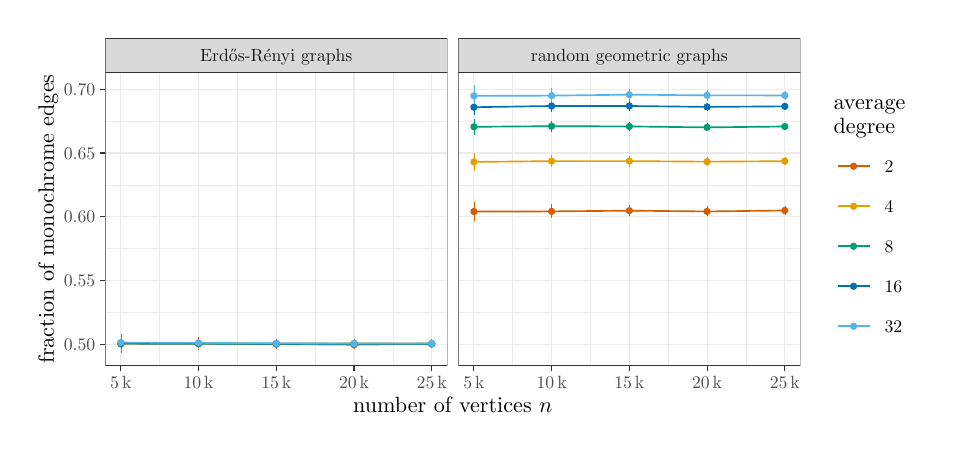
\begin{tikzpicture}[x=1pt,y=1pt]
\definecolor{fillColor}{RGB}{255,255,255}
\path[use as bounding box,fill=fillColor,fill opacity=0.00] (0,0) rectangle (325.21,144.54);
\begin{scope}
\path[clip] (  0.00,  0.00) rectangle (325.21,144.54);
\definecolor{drawColor}{RGB}{255,255,255}
\definecolor{fillColor}{RGB}{255,255,255}

\path[draw=drawColor,line width= 0.4pt,line join=round,line cap=round,fill=fillColor] (  0.00,  0.00) rectangle (325.21,144.54);
\end{scope}
\begin{scope}
\path[clip] ( 28.04, 22.32) rectangle (151.62,128.49);
\definecolor{fillColor}{RGB}{255,255,255}

\path[fill=fillColor] ( 28.04, 22.32) rectangle (151.62,128.49);
\definecolor{drawColor}{gray}{0.92}

\path[draw=drawColor,line width= 0.2pt,line join=round] ( 28.04, 41.72) --
	(151.62, 41.72);

\path[draw=drawColor,line width= 0.2pt,line join=round] ( 28.04, 64.73) --
	(151.62, 64.73);

\path[draw=drawColor,line width= 0.2pt,line join=round] ( 28.04, 87.74) --
	(151.62, 87.74);

\path[draw=drawColor,line width= 0.2pt,line join=round] ( 28.04,110.75) --
	(151.62,110.75);

\path[draw=drawColor,line width= 0.2pt,line join=round] ( 47.70, 22.32) --
	( 47.70,128.49);

\path[draw=drawColor,line width= 0.2pt,line join=round] ( 75.79, 22.32) --
	( 75.79,128.49);

\path[draw=drawColor,line width= 0.2pt,line join=round] (103.87, 22.32) --
	(103.87,128.49);

\path[draw=drawColor,line width= 0.2pt,line join=round] (131.96, 22.32) --
	(131.96,128.49);

\path[draw=drawColor,line width= 0.4pt,line join=round] ( 28.04, 30.21) --
	(151.62, 30.21);

\path[draw=drawColor,line width= 0.4pt,line join=round] ( 28.04, 53.22) --
	(151.62, 53.22);

\path[draw=drawColor,line width= 0.4pt,line join=round] ( 28.04, 76.24) --
	(151.62, 76.24);

\path[draw=drawColor,line width= 0.4pt,line join=round] ( 28.04, 99.25) --
	(151.62, 99.25);

\path[draw=drawColor,line width= 0.4pt,line join=round] ( 28.04,122.26) --
	(151.62,122.26);

\path[draw=drawColor,line width= 0.4pt,line join=round] ( 33.66, 22.32) --
	( 33.66,128.49);

\path[draw=drawColor,line width= 0.4pt,line join=round] ( 61.74, 22.32) --
	( 61.74,128.49);

\path[draw=drawColor,line width= 0.4pt,line join=round] ( 89.83, 22.32) --
	( 89.83,128.49);

\path[draw=drawColor,line width= 0.4pt,line join=round] (117.92, 22.32) --
	(117.92,128.49);

\path[draw=drawColor,line width= 0.4pt,line join=round] (146.00, 22.32) --
	(146.00,128.49);
\definecolor{drawColor}{RGB}{213,94,0}

\path[draw=drawColor,line width= 0.2pt,line join=round] ( 33.66, 33.88) --
	( 33.66, 33.88);

\path[draw=drawColor,line width= 0.2pt,line join=round] ( 33.66, 33.88) --
	( 33.66, 27.14);

\path[draw=drawColor,line width= 0.2pt,line join=round] ( 33.66, 27.14) --
	( 33.66, 27.14);

\path[draw=drawColor,line width= 0.2pt,line join=round] ( 61.74, 32.90) --
	( 61.74, 32.90);

\path[draw=drawColor,line width= 0.2pt,line join=round] ( 61.74, 32.90) --
	( 61.74, 27.95);

\path[draw=drawColor,line width= 0.2pt,line join=round] ( 61.74, 27.95) --
	( 61.74, 27.95);

\path[draw=drawColor,line width= 0.2pt,line join=round] ( 89.83, 32.15) --
	( 89.83, 32.15);

\path[draw=drawColor,line width= 0.2pt,line join=round] ( 89.83, 32.15) --
	( 89.83, 28.46);

\path[draw=drawColor,line width= 0.2pt,line join=round] ( 89.83, 28.46) --
	( 89.83, 28.46);

\path[draw=drawColor,line width= 0.2pt,line join=round] (117.92, 31.91) --
	(117.92, 31.91);

\path[draw=drawColor,line width= 0.2pt,line join=round] (117.92, 31.91) --
	(117.92, 28.37);

\path[draw=drawColor,line width= 0.2pt,line join=round] (117.92, 28.37) --
	(117.92, 28.37);

\path[draw=drawColor,line width= 0.2pt,line join=round] (146.00, 31.90) --
	(146.00, 31.90);

\path[draw=drawColor,line width= 0.2pt,line join=round] (146.00, 31.90) --
	(146.00, 28.66);

\path[draw=drawColor,line width= 0.2pt,line join=round] (146.00, 28.66) --
	(146.00, 28.66);
\definecolor{drawColor}{RGB}{230,159,0}

\path[draw=drawColor,line width= 0.2pt,line join=round] ( 33.66, 32.94) --
	( 33.66, 32.94);

\path[draw=drawColor,line width= 0.2pt,line join=round] ( 33.66, 32.94) --
	( 33.66, 28.18);

\path[draw=drawColor,line width= 0.2pt,line join=round] ( 33.66, 28.18) --
	( 33.66, 28.18);

\path[draw=drawColor,line width= 0.2pt,line join=round] ( 61.74, 32.04) --
	( 61.74, 32.04);

\path[draw=drawColor,line width= 0.2pt,line join=round] ( 61.74, 32.04) --
	( 61.74, 28.44);

\path[draw=drawColor,line width= 0.2pt,line join=round] ( 61.74, 28.44) --
	( 61.74, 28.44);

\path[draw=drawColor,line width= 0.2pt,line join=round] ( 89.83, 31.68) --
	( 89.83, 31.68);

\path[draw=drawColor,line width= 0.2pt,line join=round] ( 89.83, 31.68) --
	( 89.83, 28.78);

\path[draw=drawColor,line width= 0.2pt,line join=round] ( 89.83, 28.78) --
	( 89.83, 28.78);

\path[draw=drawColor,line width= 0.2pt,line join=round] (117.92, 31.68) --
	(117.92, 31.68);

\path[draw=drawColor,line width= 0.2pt,line join=round] (117.92, 31.68) --
	(117.92, 28.96);

\path[draw=drawColor,line width= 0.2pt,line join=round] (117.92, 28.96) --
	(117.92, 28.96);

\path[draw=drawColor,line width= 0.2pt,line join=round] (146.00, 31.45) --
	(146.00, 31.45);

\path[draw=drawColor,line width= 0.2pt,line join=round] (146.00, 31.45) --
	(146.00, 29.22);

\path[draw=drawColor,line width= 0.2pt,line join=round] (146.00, 29.22) --
	(146.00, 29.22);
\definecolor{drawColor}{RGB}{0,158,115}

\path[draw=drawColor,line width= 0.2pt,line join=round] ( 33.66, 32.28) --
	( 33.66, 32.28);

\path[draw=drawColor,line width= 0.2pt,line join=round] ( 33.66, 32.28) --
	( 33.66, 28.33);

\path[draw=drawColor,line width= 0.2pt,line join=round] ( 33.66, 28.33) --
	( 33.66, 28.33);

\path[draw=drawColor,line width= 0.2pt,line join=round] ( 61.74, 31.73) --
	( 61.74, 31.73);

\path[draw=drawColor,line width= 0.2pt,line join=round] ( 61.74, 31.73) --
	( 61.74, 28.94);

\path[draw=drawColor,line width= 0.2pt,line join=round] ( 61.74, 28.94) --
	( 61.74, 28.94);

\path[draw=drawColor,line width= 0.2pt,line join=round] ( 89.83, 31.29) --
	( 89.83, 31.29);

\path[draw=drawColor,line width= 0.2pt,line join=round] ( 89.83, 31.29) --
	( 89.83, 29.24);

\path[draw=drawColor,line width= 0.2pt,line join=round] ( 89.83, 29.24) --
	( 89.83, 29.24);

\path[draw=drawColor,line width= 0.2pt,line join=round] (117.92, 31.21) --
	(117.92, 31.21);

\path[draw=drawColor,line width= 0.2pt,line join=round] (117.92, 31.21) --
	(117.92, 29.44);

\path[draw=drawColor,line width= 0.2pt,line join=round] (117.92, 29.44) --
	(117.92, 29.44);

\path[draw=drawColor,line width= 0.2pt,line join=round] (146.00, 31.06) --
	(146.00, 31.06);

\path[draw=drawColor,line width= 0.2pt,line join=round] (146.00, 31.06) --
	(146.00, 29.44);

\path[draw=drawColor,line width= 0.2pt,line join=round] (146.00, 29.44) --
	(146.00, 29.44);
\definecolor{drawColor}{RGB}{0,114,178}

\path[draw=drawColor,line width= 0.2pt,line join=round] ( 33.66, 31.94) --
	( 33.66, 31.94);

\path[draw=drawColor,line width= 0.2pt,line join=round] ( 33.66, 31.94) --
	( 33.66, 29.05);

\path[draw=drawColor,line width= 0.2pt,line join=round] ( 33.66, 29.05) --
	( 33.66, 29.05);

\path[draw=drawColor,line width= 0.2pt,line join=round] ( 61.74, 31.41) --
	( 61.74, 31.41);

\path[draw=drawColor,line width= 0.2pt,line join=round] ( 61.74, 31.41) --
	( 61.74, 29.35);

\path[draw=drawColor,line width= 0.2pt,line join=round] ( 61.74, 29.35) --
	( 61.74, 29.35);

\path[draw=drawColor,line width= 0.2pt,line join=round] ( 89.83, 31.09) --
	( 89.83, 31.09);

\path[draw=drawColor,line width= 0.2pt,line join=round] ( 89.83, 31.09) --
	( 89.83, 29.55);

\path[draw=drawColor,line width= 0.2pt,line join=round] ( 89.83, 29.55) --
	( 89.83, 29.55);

\path[draw=drawColor,line width= 0.2pt,line join=round] (117.92, 30.86) --
	(117.92, 30.86);

\path[draw=drawColor,line width= 0.2pt,line join=round] (117.92, 30.86) --
	(117.92, 29.60);

\path[draw=drawColor,line width= 0.2pt,line join=round] (117.92, 29.60) --
	(117.92, 29.60);

\path[draw=drawColor,line width= 0.2pt,line join=round] (146.00, 30.90) --
	(146.00, 30.90);

\path[draw=drawColor,line width= 0.2pt,line join=round] (146.00, 30.90) --
	(146.00, 29.71);

\path[draw=drawColor,line width= 0.2pt,line join=round] (146.00, 29.71) --
	(146.00, 29.71);
\definecolor{drawColor}{RGB}{86,180,233}

\path[draw=drawColor,line width= 0.2pt,line join=round] ( 33.66, 32.01) --
	( 33.66, 32.01);

\path[draw=drawColor,line width= 0.2pt,line join=round] ( 33.66, 32.01) --
	( 33.66, 29.70);

\path[draw=drawColor,line width= 0.2pt,line join=round] ( 33.66, 29.70) --
	( 33.66, 29.70);

\path[draw=drawColor,line width= 0.2pt,line join=round] ( 61.74, 31.42) --
	( 61.74, 31.42);

\path[draw=drawColor,line width= 0.2pt,line join=round] ( 61.74, 31.42) --
	( 61.74, 29.85);

\path[draw=drawColor,line width= 0.2pt,line join=round] ( 61.74, 29.85) --
	( 61.74, 29.85);

\path[draw=drawColor,line width= 0.2pt,line join=round] ( 89.83, 31.08) --
	( 89.83, 31.08);

\path[draw=drawColor,line width= 0.2pt,line join=round] ( 89.83, 31.08) --
	( 89.83, 29.86);

\path[draw=drawColor,line width= 0.2pt,line join=round] ( 89.83, 29.86) --
	( 89.83, 29.86);

\path[draw=drawColor,line width= 0.2pt,line join=round] (117.92, 30.91) --
	(117.92, 30.91);

\path[draw=drawColor,line width= 0.2pt,line join=round] (117.92, 30.91) --
	(117.92, 29.88);

\path[draw=drawColor,line width= 0.2pt,line join=round] (117.92, 29.88) --
	(117.92, 29.88);

\path[draw=drawColor,line width= 0.2pt,line join=round] (146.00, 30.88) --
	(146.00, 30.88);

\path[draw=drawColor,line width= 0.2pt,line join=round] (146.00, 30.88) --
	(146.00, 29.92);

\path[draw=drawColor,line width= 0.2pt,line join=round] (146.00, 29.92) --
	(146.00, 29.92);
\definecolor{drawColor}{RGB}{213,94,0}

\path[draw=drawColor,line width= 0.6pt,line join=round] ( 33.66, 30.44) --
	( 61.74, 30.47) --
	( 89.83, 30.21) --
	(117.92, 29.97) --
	(146.00, 30.32);
\definecolor{drawColor}{RGB}{230,159,0}

\path[draw=drawColor,line width= 0.6pt,line join=round] ( 33.66, 30.36) --
	( 61.74, 30.33) --
	( 89.83, 30.29) --
	(117.92, 30.41) --
	(146.00, 30.41);
\definecolor{drawColor}{RGB}{0,158,115}

\path[draw=drawColor,line width= 0.6pt,line join=round] ( 33.66, 30.36) --
	( 61.74, 30.37) --
	( 89.83, 30.30) --
	(117.92, 30.34) --
	(146.00, 30.25);
\definecolor{drawColor}{RGB}{0,114,178}

\path[draw=drawColor,line width= 0.6pt,line join=round] ( 33.66, 30.46) --
	( 61.74, 30.39) --
	( 89.83, 30.33) --
	(117.92, 30.28) --
	(146.00, 30.30);
\definecolor{drawColor}{RGB}{86,180,233}

\path[draw=drawColor,line width= 0.6pt,line join=round] ( 33.66, 30.76) --
	( 61.74, 30.64) --
	( 89.83, 30.47) --
	(117.92, 30.39) --
	(146.00, 30.39);
\definecolor{drawColor}{RGB}{213,94,0}
\definecolor{fillColor}{RGB}{213,94,0}

\path[draw=drawColor,line width= 0.4pt,line join=round,line cap=round,fill=fillColor] ( 33.66, 30.44) circle (  1.11);

\path[draw=drawColor,line width= 0.4pt,line join=round,line cap=round,fill=fillColor] ( 61.74, 30.47) circle (  1.11);

\path[draw=drawColor,line width= 0.4pt,line join=round,line cap=round,fill=fillColor] ( 89.83, 30.21) circle (  1.11);

\path[draw=drawColor,line width= 0.4pt,line join=round,line cap=round,fill=fillColor] (117.92, 29.97) circle (  1.11);

\path[draw=drawColor,line width= 0.4pt,line join=round,line cap=round,fill=fillColor] (146.00, 30.32) circle (  1.11);
\definecolor{drawColor}{RGB}{230,159,0}
\definecolor{fillColor}{RGB}{230,159,0}

\path[draw=drawColor,line width= 0.4pt,line join=round,line cap=round,fill=fillColor] ( 33.66, 30.36) circle (  1.11);

\path[draw=drawColor,line width= 0.4pt,line join=round,line cap=round,fill=fillColor] ( 61.74, 30.33) circle (  1.11);

\path[draw=drawColor,line width= 0.4pt,line join=round,line cap=round,fill=fillColor] ( 89.83, 30.29) circle (  1.11);

\path[draw=drawColor,line width= 0.4pt,line join=round,line cap=round,fill=fillColor] (117.92, 30.41) circle (  1.11);

\path[draw=drawColor,line width= 0.4pt,line join=round,line cap=round,fill=fillColor] (146.00, 30.41) circle (  1.11);
\definecolor{drawColor}{RGB}{0,158,115}
\definecolor{fillColor}{RGB}{0,158,115}

\path[draw=drawColor,line width= 0.4pt,line join=round,line cap=round,fill=fillColor] ( 33.66, 30.36) circle (  1.11);

\path[draw=drawColor,line width= 0.4pt,line join=round,line cap=round,fill=fillColor] ( 61.74, 30.37) circle (  1.11);

\path[draw=drawColor,line width= 0.4pt,line join=round,line cap=round,fill=fillColor] ( 89.83, 30.30) circle (  1.11);

\path[draw=drawColor,line width= 0.4pt,line join=round,line cap=round,fill=fillColor] (117.92, 30.34) circle (  1.11);

\path[draw=drawColor,line width= 0.4pt,line join=round,line cap=round,fill=fillColor] (146.00, 30.25) circle (  1.11);
\definecolor{drawColor}{RGB}{0,114,178}
\definecolor{fillColor}{RGB}{0,114,178}

\path[draw=drawColor,line width= 0.4pt,line join=round,line cap=round,fill=fillColor] ( 33.66, 30.46) circle (  1.11);

\path[draw=drawColor,line width= 0.4pt,line join=round,line cap=round,fill=fillColor] ( 61.74, 30.39) circle (  1.11);

\path[draw=drawColor,line width= 0.4pt,line join=round,line cap=round,fill=fillColor] ( 89.83, 30.33) circle (  1.11);

\path[draw=drawColor,line width= 0.4pt,line join=round,line cap=round,fill=fillColor] (117.92, 30.28) circle (  1.11);

\path[draw=drawColor,line width= 0.4pt,line join=round,line cap=round,fill=fillColor] (146.00, 30.30) circle (  1.11);
\definecolor{drawColor}{RGB}{86,180,233}
\definecolor{fillColor}{RGB}{86,180,233}

\path[draw=drawColor,line width= 0.4pt,line join=round,line cap=round,fill=fillColor] ( 33.66, 30.76) circle (  1.11);

\path[draw=drawColor,line width= 0.4pt,line join=round,line cap=round,fill=fillColor] ( 61.74, 30.64) circle (  1.11);

\path[draw=drawColor,line width= 0.4pt,line join=round,line cap=round,fill=fillColor] ( 89.83, 30.47) circle (  1.11);

\path[draw=drawColor,line width= 0.4pt,line join=round,line cap=round,fill=fillColor] (117.92, 30.39) circle (  1.11);

\path[draw=drawColor,line width= 0.4pt,line join=round,line cap=round,fill=fillColor] (146.00, 30.39) circle (  1.11);
\definecolor{drawColor}{gray}{0.20}

\path[draw=drawColor,line width= 0.4pt,line join=round,line cap=round] ( 28.04, 22.32) rectangle (151.62,128.49);
\end{scope}
\begin{scope}
\path[clip] (155.62, 22.32) rectangle (279.20,128.49);
\definecolor{fillColor}{RGB}{255,255,255}

\path[fill=fillColor] (155.62, 22.32) rectangle (279.20,128.49);
\definecolor{drawColor}{gray}{0.92}

\path[draw=drawColor,line width= 0.2pt,line join=round] (155.62, 41.72) --
	(279.20, 41.72);

\path[draw=drawColor,line width= 0.2pt,line join=round] (155.62, 64.73) --
	(279.20, 64.73);

\path[draw=drawColor,line width= 0.2pt,line join=round] (155.62, 87.74) --
	(279.20, 87.74);

\path[draw=drawColor,line width= 0.2pt,line join=round] (155.62,110.75) --
	(279.20,110.75);

\path[draw=drawColor,line width= 0.2pt,line join=round] (175.28, 22.32) --
	(175.28,128.49);

\path[draw=drawColor,line width= 0.2pt,line join=round] (203.37, 22.32) --
	(203.37,128.49);

\path[draw=drawColor,line width= 0.2pt,line join=round] (231.45, 22.32) --
	(231.45,128.49);

\path[draw=drawColor,line width= 0.2pt,line join=round] (259.54, 22.32) --
	(259.54,128.49);

\path[draw=drawColor,line width= 0.4pt,line join=round] (155.62, 30.21) --
	(279.20, 30.21);

\path[draw=drawColor,line width= 0.4pt,line join=round] (155.62, 53.22) --
	(279.20, 53.22);

\path[draw=drawColor,line width= 0.4pt,line join=round] (155.62, 76.24) --
	(279.20, 76.24);

\path[draw=drawColor,line width= 0.4pt,line join=round] (155.62, 99.25) --
	(279.20, 99.25);

\path[draw=drawColor,line width= 0.4pt,line join=round] (155.62,122.26) --
	(279.20,122.26);

\path[draw=drawColor,line width= 0.4pt,line join=round] (161.24, 22.32) --
	(161.24,128.49);

\path[draw=drawColor,line width= 0.4pt,line join=round] (189.32, 22.32) --
	(189.32,128.49);

\path[draw=drawColor,line width= 0.4pt,line join=round] (217.41, 22.32) --
	(217.41,128.49);

\path[draw=drawColor,line width= 0.4pt,line join=round] (245.50, 22.32) --
	(245.50,128.49);

\path[draw=drawColor,line width= 0.4pt,line join=round] (273.58, 22.32) --
	(273.58,128.49);
\definecolor{drawColor}{RGB}{213,94,0}

\path[draw=drawColor,line width= 0.2pt,line join=round] (161.24, 81.72) --
	(161.24, 81.72);

\path[draw=drawColor,line width= 0.2pt,line join=round] (161.24, 81.72) --
	(161.24, 74.65);

\path[draw=drawColor,line width= 0.2pt,line join=round] (161.24, 74.65) --
	(161.24, 74.65);

\path[draw=drawColor,line width= 0.2pt,line join=round] (189.32, 80.87) --
	(189.32, 80.87);

\path[draw=drawColor,line width= 0.2pt,line join=round] (189.32, 80.87) --
	(189.32, 75.64);

\path[draw=drawColor,line width= 0.2pt,line join=round] (189.32, 75.64) --
	(189.32, 75.64);

\path[draw=drawColor,line width= 0.2pt,line join=round] (217.41, 80.63) --
	(217.41, 80.63);

\path[draw=drawColor,line width= 0.2pt,line join=round] (217.41, 80.63) --
	(217.41, 76.34);

\path[draw=drawColor,line width= 0.2pt,line join=round] (217.41, 76.34) --
	(217.41, 76.34);

\path[draw=drawColor,line width= 0.2pt,line join=round] (245.50, 80.06) --
	(245.50, 80.06);

\path[draw=drawColor,line width= 0.2pt,line join=round] (245.50, 80.06) --
	(245.50, 76.51);

\path[draw=drawColor,line width= 0.2pt,line join=round] (245.50, 76.51) --
	(245.50, 76.51);

\path[draw=drawColor,line width= 0.2pt,line join=round] (273.58, 79.98) --
	(273.58, 79.98);

\path[draw=drawColor,line width= 0.2pt,line join=round] (273.58, 79.98) --
	(273.58, 76.91);

\path[draw=drawColor,line width= 0.2pt,line join=round] (273.58, 76.91) --
	(273.58, 76.91);
\definecolor{drawColor}{RGB}{230,159,0}

\path[draw=drawColor,line width= 0.2pt,line join=round] (161.24, 99.28) --
	(161.24, 99.28);

\path[draw=drawColor,line width= 0.2pt,line join=round] (161.24, 99.28) --
	(161.24, 92.87);

\path[draw=drawColor,line width= 0.2pt,line join=round] (161.24, 92.87) --
	(161.24, 92.87);

\path[draw=drawColor,line width= 0.2pt,line join=round] (189.32, 98.49) --
	(189.32, 98.49);

\path[draw=drawColor,line width= 0.2pt,line join=round] (189.32, 98.49) --
	(189.32, 94.02);

\path[draw=drawColor,line width= 0.2pt,line join=round] (189.32, 94.02) --
	(189.32, 94.02);

\path[draw=drawColor,line width= 0.2pt,line join=round] (217.41, 97.99) --
	(217.41, 97.99);

\path[draw=drawColor,line width= 0.2pt,line join=round] (217.41, 97.99) --
	(217.41, 94.35);

\path[draw=drawColor,line width= 0.2pt,line join=round] (217.41, 94.35) --
	(217.41, 94.35);

\path[draw=drawColor,line width= 0.2pt,line join=round] (245.50, 97.64) --
	(245.50, 97.64);

\path[draw=drawColor,line width= 0.2pt,line join=round] (245.50, 97.64) --
	(245.50, 94.60);

\path[draw=drawColor,line width= 0.2pt,line join=round] (245.50, 94.60) --
	(245.50, 94.60);

\path[draw=drawColor,line width= 0.2pt,line join=round] (273.58, 97.79) --
	(273.58, 97.79);

\path[draw=drawColor,line width= 0.2pt,line join=round] (273.58, 97.79) --
	(273.58, 94.94);

\path[draw=drawColor,line width= 0.2pt,line join=round] (273.58, 94.94) --
	(273.58, 94.94);
\definecolor{drawColor}{RGB}{0,158,115}

\path[draw=drawColor,line width= 0.2pt,line join=round] (161.24,111.65) --
	(161.24,111.65);

\path[draw=drawColor,line width= 0.2pt,line join=round] (161.24,111.65) --
	(161.24,105.83);

\path[draw=drawColor,line width= 0.2pt,line join=round] (161.24,105.83) --
	(161.24,105.83);

\path[draw=drawColor,line width= 0.2pt,line join=round] (189.32,110.93) --
	(189.32,110.93);

\path[draw=drawColor,line width= 0.2pt,line join=round] (189.32,110.93) --
	(189.32,106.76);

\path[draw=drawColor,line width= 0.2pt,line join=round] (189.32,106.76) --
	(189.32,106.76);

\path[draw=drawColor,line width= 0.2pt,line join=round] (217.41,110.63) --
	(217.41,110.63);

\path[draw=drawColor,line width= 0.2pt,line join=round] (217.41,110.63) --
	(217.41,107.16);

\path[draw=drawColor,line width= 0.2pt,line join=round] (217.41,107.16) --
	(217.41,107.16);

\path[draw=drawColor,line width= 0.2pt,line join=round] (245.50,110.04) --
	(245.50,110.04);

\path[draw=drawColor,line width= 0.2pt,line join=round] (245.50,110.04) --
	(245.50,107.09);

\path[draw=drawColor,line width= 0.2pt,line join=round] (245.50,107.09) --
	(245.50,107.09);

\path[draw=drawColor,line width= 0.2pt,line join=round] (273.58,110.05) --
	(273.58,110.05);

\path[draw=drawColor,line width= 0.2pt,line join=round] (273.58,110.05) --
	(273.58,107.44);

\path[draw=drawColor,line width= 0.2pt,line join=round] (273.58,107.44) --
	(273.58,107.44);
\definecolor{drawColor}{RGB}{0,114,178}

\path[draw=drawColor,line width= 0.2pt,line join=round] (161.24,119.01) --
	(161.24,119.01);

\path[draw=drawColor,line width= 0.2pt,line join=round] (161.24,119.01) --
	(161.24,112.85);

\path[draw=drawColor,line width= 0.2pt,line join=round] (161.24,112.85) --
	(161.24,112.85);

\path[draw=drawColor,line width= 0.2pt,line join=round] (189.32,118.44) --
	(189.32,118.44);

\path[draw=drawColor,line width= 0.2pt,line join=round] (189.32,118.44) --
	(189.32,114.03);

\path[draw=drawColor,line width= 0.2pt,line join=round] (189.32,114.03) --
	(189.32,114.03);

\path[draw=drawColor,line width= 0.2pt,line join=round] (217.41,118.24) --
	(217.41,118.24);

\path[draw=drawColor,line width= 0.2pt,line join=round] (217.41,118.24) --
	(217.41,114.52);

\path[draw=drawColor,line width= 0.2pt,line join=round] (217.41,114.52) --
	(217.41,114.52);

\path[draw=drawColor,line width= 0.2pt,line join=round] (245.50,117.41) --
	(245.50,117.41);

\path[draw=drawColor,line width= 0.2pt,line join=round] (245.50,117.41) --
	(245.50,114.57);

\path[draw=drawColor,line width= 0.2pt,line join=round] (245.50,114.57) --
	(245.50,114.57);

\path[draw=drawColor,line width= 0.2pt,line join=round] (273.58,117.44) --
	(273.58,117.44);

\path[draw=drawColor,line width= 0.2pt,line join=round] (273.58,117.44) --
	(273.58,114.71);

\path[draw=drawColor,line width= 0.2pt,line join=round] (273.58,114.71) --
	(273.58,114.71);
\definecolor{drawColor}{RGB}{86,180,233}

\path[draw=drawColor,line width= 0.2pt,line join=round] (161.24,123.66) --
	(161.24,123.66);

\path[draw=drawColor,line width= 0.2pt,line join=round] (161.24,123.66) --
	(161.24,116.31);

\path[draw=drawColor,line width= 0.2pt,line join=round] (161.24,116.31) --
	(161.24,116.31);

\path[draw=drawColor,line width= 0.2pt,line join=round] (189.32,122.69) --
	(189.32,122.69);

\path[draw=drawColor,line width= 0.2pt,line join=round] (189.32,122.69) --
	(189.32,117.31);

\path[draw=drawColor,line width= 0.2pt,line join=round] (189.32,117.31) --
	(189.32,117.31);

\path[draw=drawColor,line width= 0.2pt,line join=round] (217.41,122.42) --
	(217.41,122.42);

\path[draw=drawColor,line width= 0.2pt,line join=round] (217.41,122.42) --
	(217.41,118.10);

\path[draw=drawColor,line width= 0.2pt,line join=round] (217.41,118.10) --
	(217.41,118.10);

\path[draw=drawColor,line width= 0.2pt,line join=round] (245.50,121.89) --
	(245.50,121.89);

\path[draw=drawColor,line width= 0.2pt,line join=round] (245.50,121.89) --
	(245.50,118.22);

\path[draw=drawColor,line width= 0.2pt,line join=round] (245.50,118.22) --
	(245.50,118.22);

\path[draw=drawColor,line width= 0.2pt,line join=round] (273.58,121.65) --
	(273.58,121.65);

\path[draw=drawColor,line width= 0.2pt,line join=round] (273.58,121.65) --
	(273.58,118.32);

\path[draw=drawColor,line width= 0.2pt,line join=round] (273.58,118.32) --
	(273.58,118.32);
\definecolor{drawColor}{RGB}{213,94,0}

\path[draw=drawColor,line width= 0.6pt,line join=round] (161.24, 78.09) --
	(189.32, 78.15) --
	(217.41, 78.41) --
	(245.50, 78.13) --
	(273.58, 78.48);
\definecolor{drawColor}{RGB}{230,159,0}

\path[draw=drawColor,line width= 0.6pt,line join=round] (161.24, 96.02) --
	(189.32, 96.32) --
	(217.41, 96.32) --
	(245.50, 96.12) --
	(273.58, 96.30);
\definecolor{drawColor}{RGB}{0,158,115}

\path[draw=drawColor,line width= 0.6pt,line join=round] (161.24,108.71) --
	(189.32,108.95) --
	(217.41,108.85) --
	(245.50,108.51) --
	(273.58,108.83);
\definecolor{drawColor}{RGB}{0,114,178}

\path[draw=drawColor,line width= 0.6pt,line join=round] (161.24,115.80) --
	(189.32,116.24) --
	(217.41,116.24) --
	(245.50,115.91) --
	(273.58,116.11);
\definecolor{drawColor}{RGB}{86,180,233}

\path[draw=drawColor,line width= 0.6pt,line join=round] (161.24,119.89) --
	(189.32,119.98) --
	(217.41,120.33) --
	(245.50,120.08) --
	(273.58,120.05);
\definecolor{drawColor}{RGB}{213,94,0}
\definecolor{fillColor}{RGB}{213,94,0}

\path[draw=drawColor,line width= 0.4pt,line join=round,line cap=round,fill=fillColor] (161.24, 78.09) circle (  1.11);

\path[draw=drawColor,line width= 0.4pt,line join=round,line cap=round,fill=fillColor] (189.32, 78.15) circle (  1.11);

\path[draw=drawColor,line width= 0.4pt,line join=round,line cap=round,fill=fillColor] (217.41, 78.41) circle (  1.11);

\path[draw=drawColor,line width= 0.4pt,line join=round,line cap=round,fill=fillColor] (245.50, 78.13) circle (  1.11);

\path[draw=drawColor,line width= 0.4pt,line join=round,line cap=round,fill=fillColor] (273.58, 78.48) circle (  1.11);
\definecolor{drawColor}{RGB}{230,159,0}
\definecolor{fillColor}{RGB}{230,159,0}

\path[draw=drawColor,line width= 0.4pt,line join=round,line cap=round,fill=fillColor] (161.24, 96.02) circle (  1.11);

\path[draw=drawColor,line width= 0.4pt,line join=round,line cap=round,fill=fillColor] (189.32, 96.32) circle (  1.11);

\path[draw=drawColor,line width= 0.4pt,line join=round,line cap=round,fill=fillColor] (217.41, 96.32) circle (  1.11);

\path[draw=drawColor,line width= 0.4pt,line join=round,line cap=round,fill=fillColor] (245.50, 96.12) circle (  1.11);

\path[draw=drawColor,line width= 0.4pt,line join=round,line cap=round,fill=fillColor] (273.58, 96.30) circle (  1.11);
\definecolor{drawColor}{RGB}{0,158,115}
\definecolor{fillColor}{RGB}{0,158,115}

\path[draw=drawColor,line width= 0.4pt,line join=round,line cap=round,fill=fillColor] (161.24,108.71) circle (  1.11);

\path[draw=drawColor,line width= 0.4pt,line join=round,line cap=round,fill=fillColor] (189.32,108.95) circle (  1.11);

\path[draw=drawColor,line width= 0.4pt,line join=round,line cap=round,fill=fillColor] (217.41,108.85) circle (  1.11);

\path[draw=drawColor,line width= 0.4pt,line join=round,line cap=round,fill=fillColor] (245.50,108.51) circle (  1.11);

\path[draw=drawColor,line width= 0.4pt,line join=round,line cap=round,fill=fillColor] (273.58,108.83) circle (  1.11);
\definecolor{drawColor}{RGB}{0,114,178}
\definecolor{fillColor}{RGB}{0,114,178}

\path[draw=drawColor,line width= 0.4pt,line join=round,line cap=round,fill=fillColor] (161.24,115.80) circle (  1.11);

\path[draw=drawColor,line width= 0.4pt,line join=round,line cap=round,fill=fillColor] (189.32,116.24) circle (  1.11);

\path[draw=drawColor,line width= 0.4pt,line join=round,line cap=round,fill=fillColor] (217.41,116.24) circle (  1.11);

\path[draw=drawColor,line width= 0.4pt,line join=round,line cap=round,fill=fillColor] (245.50,115.91) circle (  1.11);

\path[draw=drawColor,line width= 0.4pt,line join=round,line cap=round,fill=fillColor] (273.58,116.11) circle (  1.11);
\definecolor{drawColor}{RGB}{86,180,233}
\definecolor{fillColor}{RGB}{86,180,233}

\path[draw=drawColor,line width= 0.4pt,line join=round,line cap=round,fill=fillColor] (161.24,119.89) circle (  1.11);

\path[draw=drawColor,line width= 0.4pt,line join=round,line cap=round,fill=fillColor] (189.32,119.98) circle (  1.11);

\path[draw=drawColor,line width= 0.4pt,line join=round,line cap=round,fill=fillColor] (217.41,120.33) circle (  1.11);

\path[draw=drawColor,line width= 0.4pt,line join=round,line cap=round,fill=fillColor] (245.50,120.08) circle (  1.11);

\path[draw=drawColor,line width= 0.4pt,line join=round,line cap=round,fill=fillColor] (273.58,120.05) circle (  1.11);
\definecolor{drawColor}{gray}{0.20}

\path[draw=drawColor,line width= 0.4pt,line join=round,line cap=round] (155.62, 22.32) rectangle (279.20,128.49);
\end{scope}
\begin{scope}
\path[clip] ( 28.04,128.49) rectangle (151.62,140.54);
\definecolor{drawColor}{gray}{0.20}
\definecolor{fillColor}{gray}{0.85}

\path[draw=drawColor,line width= 0.4pt,line join=round,line cap=round,fill=fillColor] ( 28.04,128.49) rectangle (151.62,140.54);
\definecolor{drawColor}{gray}{0.10}

\node[text=drawColor,anchor=base,inner sep=0pt, outer sep=0pt, scale=  0.64] at ( 89.83,132.31) {Erd{\H o}s-R\'enyi graphs};
\end{scope}
\begin{scope}
\path[clip] (155.62,128.49) rectangle (279.20,140.54);
\definecolor{drawColor}{gray}{0.20}
\definecolor{fillColor}{gray}{0.85}

\path[draw=drawColor,line width= 0.4pt,line join=round,line cap=round,fill=fillColor] (155.62,128.49) rectangle (279.20,140.54);
\definecolor{drawColor}{gray}{0.10}

\node[text=drawColor,anchor=base,inner sep=0pt, outer sep=0pt, scale=  0.64] at (217.41,132.31) {random geometric graphs};
\end{scope}
\begin{scope}
\path[clip] (  0.00,  0.00) rectangle (325.21,144.54);
\definecolor{drawColor}{gray}{0.20}

\path[draw=drawColor,line width= 0.4pt,line join=round] ( 33.66, 20.32) --
	( 33.66, 22.32);

\path[draw=drawColor,line width= 0.4pt,line join=round] ( 61.74, 20.32) --
	( 61.74, 22.32);

\path[draw=drawColor,line width= 0.4pt,line join=round] ( 89.83, 20.32) --
	( 89.83, 22.32);

\path[draw=drawColor,line width= 0.4pt,line join=round] (117.92, 20.32) --
	(117.92, 22.32);

\path[draw=drawColor,line width= 0.4pt,line join=round] (146.00, 20.32) --
	(146.00, 22.32);
\end{scope}
\begin{scope}
\path[clip] (  0.00,  0.00) rectangle (325.21,144.54);
\definecolor{drawColor}{gray}{0.30}

\node[text=drawColor,anchor=base,inner sep=0pt, outer sep=0pt, scale=  0.64] at ( 33.66, 14.31) {5\,k};

\node[text=drawColor,anchor=base,inner sep=0pt, outer sep=0pt, scale=  0.64] at ( 61.74, 14.31) {10\,k};

\node[text=drawColor,anchor=base,inner sep=0pt, outer sep=0pt, scale=  0.64] at ( 89.83, 14.31) {15\,k};

\node[text=drawColor,anchor=base,inner sep=0pt, outer sep=0pt, scale=  0.64] at (117.92, 14.31) {20\,k};

\node[text=drawColor,anchor=base,inner sep=0pt, outer sep=0pt, scale=  0.64] at (146.00, 14.31) {25\,k};
\end{scope}
\begin{scope}
\path[clip] (  0.00,  0.00) rectangle (325.21,144.54);
\definecolor{drawColor}{gray}{0.20}

\path[draw=drawColor,line width= 0.4pt,line join=round] (161.24, 20.32) --
	(161.24, 22.32);

\path[draw=drawColor,line width= 0.4pt,line join=round] (189.32, 20.32) --
	(189.32, 22.32);

\path[draw=drawColor,line width= 0.4pt,line join=round] (217.41, 20.32) --
	(217.41, 22.32);

\path[draw=drawColor,line width= 0.4pt,line join=round] (245.50, 20.32) --
	(245.50, 22.32);

\path[draw=drawColor,line width= 0.4pt,line join=round] (273.58, 20.32) --
	(273.58, 22.32);
\end{scope}
\begin{scope}
\path[clip] (  0.00,  0.00) rectangle (325.21,144.54);
\definecolor{drawColor}{gray}{0.30}

\node[text=drawColor,anchor=base,inner sep=0pt, outer sep=0pt, scale=  0.64] at (161.24, 14.31) {5\,k};

\node[text=drawColor,anchor=base,inner sep=0pt, outer sep=0pt, scale=  0.64] at (189.32, 14.31) {10\,k};

\node[text=drawColor,anchor=base,inner sep=0pt, outer sep=0pt, scale=  0.64] at (217.41, 14.31) {15\,k};

\node[text=drawColor,anchor=base,inner sep=0pt, outer sep=0pt, scale=  0.64] at (245.50, 14.31) {20\,k};

\node[text=drawColor,anchor=base,inner sep=0pt, outer sep=0pt, scale=  0.64] at (273.58, 14.31) {25\,k};
\end{scope}
\begin{scope}
\path[clip] (  0.00,  0.00) rectangle (325.21,144.54);
\definecolor{drawColor}{gray}{0.30}

\node[text=drawColor,anchor=base east,inner sep=0pt, outer sep=0pt, scale=  0.64] at ( 24.44, 28.01) {0.50};

\node[text=drawColor,anchor=base east,inner sep=0pt, outer sep=0pt, scale=  0.64] at ( 24.44, 51.02) {0.55};

\node[text=drawColor,anchor=base east,inner sep=0pt, outer sep=0pt, scale=  0.64] at ( 24.44, 74.03) {0.60};

\node[text=drawColor,anchor=base east,inner sep=0pt, outer sep=0pt, scale=  0.64] at ( 24.44, 97.04) {0.65};

\node[text=drawColor,anchor=base east,inner sep=0pt, outer sep=0pt, scale=  0.64] at ( 24.44,120.05) {0.70};
\end{scope}
\begin{scope}
\path[clip] (  0.00,  0.00) rectangle (325.21,144.54);
\definecolor{drawColor}{gray}{0.20}

\path[draw=drawColor,line width= 0.4pt,line join=round] ( 26.04, 30.21) --
	( 28.04, 30.21);

\path[draw=drawColor,line width= 0.4pt,line join=round] ( 26.04, 53.22) --
	( 28.04, 53.22);

\path[draw=drawColor,line width= 0.4pt,line join=round] ( 26.04, 76.24) --
	( 28.04, 76.24);

\path[draw=drawColor,line width= 0.4pt,line join=round] ( 26.04, 99.25) --
	( 28.04, 99.25);

\path[draw=drawColor,line width= 0.4pt,line join=round] ( 26.04,122.26) --
	( 28.04,122.26);
\end{scope}
\begin{scope}
\path[clip] (  0.00,  0.00) rectangle (325.21,144.54);
\definecolor{drawColor}{RGB}{0,0,0}

\node[text=drawColor,anchor=base,inner sep=0pt, outer sep=0pt, scale=  0.80] at (153.62,  5.56) {number of vertices $n$};
\end{scope}
\begin{scope}
\path[clip] (  0.00,  0.00) rectangle (325.21,144.54);
\definecolor{drawColor}{RGB}{0,0,0}

\node[text=drawColor,rotate= 90.00,anchor=base,inner sep=0pt, outer sep=0pt, scale=  0.80] at (  9.51, 75.40) {fraction of monochrome edges};
\end{scope}
\begin{scope}
\path[clip] (  0.00,  0.00) rectangle (325.21,144.54);
\definecolor{fillColor}{RGB}{255,255,255}

\path[fill=fillColor] (287.20, 25.42) rectangle (321.21,125.39);
\end{scope}
\begin{scope}
\path[clip] (  0.00,  0.00) rectangle (325.21,144.54);
\definecolor{drawColor}{RGB}{0,0,0}

\node[text=drawColor,anchor=base west,inner sep=0pt, outer sep=0pt, scale=  0.80] at (291.20,115.10) {average};

\node[text=drawColor,anchor=base west,inner sep=0pt, outer sep=0pt, scale=  0.80] at (291.20,106.46) {degree};
\end{scope}
\begin{scope}
\path[clip] (  0.00,  0.00) rectangle (325.21,144.54);
\definecolor{fillColor}{RGB}{255,255,255}

\path[fill=fillColor] (291.20, 87.23) rectangle (305.65,101.69);
\end{scope}
\begin{scope}
\path[clip] (  0.00,  0.00) rectangle (325.21,144.54);
\definecolor{drawColor}{RGB}{213,94,0}

\path[draw=drawColor,line width= 0.2pt,line join=round] (292.64, 94.46) -- (304.21, 94.46);
\end{scope}
\begin{scope}
\path[clip] (  0.00,  0.00) rectangle (325.21,144.54);
\definecolor{drawColor}{RGB}{213,94,0}

\path[draw=drawColor,line width= 0.6pt,line join=round] (292.64, 94.46) -- (304.21, 94.46);
\end{scope}
\begin{scope}
\path[clip] (  0.00,  0.00) rectangle (325.21,144.54);
\definecolor{drawColor}{RGB}{213,94,0}
\definecolor{fillColor}{RGB}{213,94,0}

\path[draw=drawColor,line width= 0.4pt,line join=round,line cap=round,fill=fillColor] (298.43, 94.46) circle (  1.11);
\end{scope}
\begin{scope}
\path[clip] (  0.00,  0.00) rectangle (325.21,144.54);
\definecolor{fillColor}{RGB}{255,255,255}

\path[fill=fillColor] (291.20, 72.78) rectangle (305.65, 87.23);
\end{scope}
\begin{scope}
\path[clip] (  0.00,  0.00) rectangle (325.21,144.54);
\definecolor{drawColor}{RGB}{230,159,0}

\path[draw=drawColor,line width= 0.2pt,line join=round] (292.64, 80.00) -- (304.21, 80.00);
\end{scope}
\begin{scope}
\path[clip] (  0.00,  0.00) rectangle (325.21,144.54);
\definecolor{drawColor}{RGB}{230,159,0}

\path[draw=drawColor,line width= 0.6pt,line join=round] (292.64, 80.00) -- (304.21, 80.00);
\end{scope}
\begin{scope}
\path[clip] (  0.00,  0.00) rectangle (325.21,144.54);
\definecolor{drawColor}{RGB}{230,159,0}
\definecolor{fillColor}{RGB}{230,159,0}

\path[draw=drawColor,line width= 0.4pt,line join=round,line cap=round,fill=fillColor] (298.43, 80.00) circle (  1.11);
\end{scope}
\begin{scope}
\path[clip] (  0.00,  0.00) rectangle (325.21,144.54);
\definecolor{fillColor}{RGB}{255,255,255}

\path[fill=fillColor] (291.20, 58.32) rectangle (305.65, 72.78);
\end{scope}
\begin{scope}
\path[clip] (  0.00,  0.00) rectangle (325.21,144.54);
\definecolor{drawColor}{RGB}{0,158,115}

\path[draw=drawColor,line width= 0.2pt,line join=round] (292.64, 65.55) -- (304.21, 65.55);
\end{scope}
\begin{scope}
\path[clip] (  0.00,  0.00) rectangle (325.21,144.54);
\definecolor{drawColor}{RGB}{0,158,115}

\path[draw=drawColor,line width= 0.6pt,line join=round] (292.64, 65.55) -- (304.21, 65.55);
\end{scope}
\begin{scope}
\path[clip] (  0.00,  0.00) rectangle (325.21,144.54);
\definecolor{drawColor}{RGB}{0,158,115}
\definecolor{fillColor}{RGB}{0,158,115}

\path[draw=drawColor,line width= 0.4pt,line join=round,line cap=round,fill=fillColor] (298.43, 65.55) circle (  1.11);
\end{scope}
\begin{scope}
\path[clip] (  0.00,  0.00) rectangle (325.21,144.54);
\definecolor{fillColor}{RGB}{255,255,255}

\path[fill=fillColor] (291.20, 43.87) rectangle (305.65, 58.32);
\end{scope}
\begin{scope}
\path[clip] (  0.00,  0.00) rectangle (325.21,144.54);
\definecolor{drawColor}{RGB}{0,114,178}

\path[draw=drawColor,line width= 0.2pt,line join=round] (292.64, 51.10) -- (304.21, 51.10);
\end{scope}
\begin{scope}
\path[clip] (  0.00,  0.00) rectangle (325.21,144.54);
\definecolor{drawColor}{RGB}{0,114,178}

\path[draw=drawColor,line width= 0.6pt,line join=round] (292.64, 51.10) -- (304.21, 51.10);
\end{scope}
\begin{scope}
\path[clip] (  0.00,  0.00) rectangle (325.21,144.54);
\definecolor{drawColor}{RGB}{0,114,178}
\definecolor{fillColor}{RGB}{0,114,178}

\path[draw=drawColor,line width= 0.4pt,line join=round,line cap=round,fill=fillColor] (298.43, 51.10) circle (  1.11);
\end{scope}
\begin{scope}
\path[clip] (  0.00,  0.00) rectangle (325.21,144.54);
\definecolor{fillColor}{RGB}{255,255,255}

\path[fill=fillColor] (291.20, 29.42) rectangle (305.65, 43.87);
\end{scope}
\begin{scope}
\path[clip] (  0.00,  0.00) rectangle (325.21,144.54);
\definecolor{drawColor}{RGB}{86,180,233}

\path[draw=drawColor,line width= 0.2pt,line join=round] (292.64, 36.64) -- (304.21, 36.64);
\end{scope}
\begin{scope}
\path[clip] (  0.00,  0.00) rectangle (325.21,144.54);
\definecolor{drawColor}{RGB}{86,180,233}

\path[draw=drawColor,line width= 0.6pt,line join=round] (292.64, 36.64) -- (304.21, 36.64);
\end{scope}
\begin{scope}
\path[clip] (  0.00,  0.00) rectangle (325.21,144.54);
\definecolor{drawColor}{RGB}{86,180,233}
\definecolor{fillColor}{RGB}{86,180,233}

\path[draw=drawColor,line width= 0.4pt,line join=round,line cap=round,fill=fillColor] (298.43, 36.64) circle (  1.11);
\end{scope}
\begin{scope}
\path[clip] (  0.00,  0.00) rectangle (325.21,144.54);
\definecolor{drawColor}{RGB}{0,0,0}

\node[text=drawColor,anchor=base west,inner sep=0pt, outer sep=0pt, scale=  0.64] at (309.65, 92.25) {2};
\end{scope}
\begin{scope}
\path[clip] (  0.00,  0.00) rectangle (325.21,144.54);
\definecolor{drawColor}{RGB}{0,0,0}

\node[text=drawColor,anchor=base west,inner sep=0pt, outer sep=0pt, scale=  0.64] at (309.65, 77.80) {4};
\end{scope}
\begin{scope}
\path[clip] (  0.00,  0.00) rectangle (325.21,144.54);
\definecolor{drawColor}{RGB}{0,0,0}

\node[text=drawColor,anchor=base west,inner sep=0pt, outer sep=0pt, scale=  0.64] at (309.65, 63.35) {8};
\end{scope}
\begin{scope}
\path[clip] (  0.00,  0.00) rectangle (325.21,144.54);
\definecolor{drawColor}{RGB}{0,0,0}

\node[text=drawColor,anchor=base west,inner sep=0pt, outer sep=0pt, scale=  0.64] at (309.65, 48.89) {16};
\end{scope}
\begin{scope}
\path[clip] (  0.00,  0.00) rectangle (325.21,144.54);
\definecolor{drawColor}{RGB}{0,0,0}

\node[text=drawColor,anchor=base west,inner sep=0pt, outer sep=0pt, scale=  0.64] at (309.65, 34.44) {32};
\end{scope}
\end{tikzpicture}

  \caption{Intro plot}
\end{figure}

\begin{figure}
  \centering
  \hspace{0.055\textwidth}%
  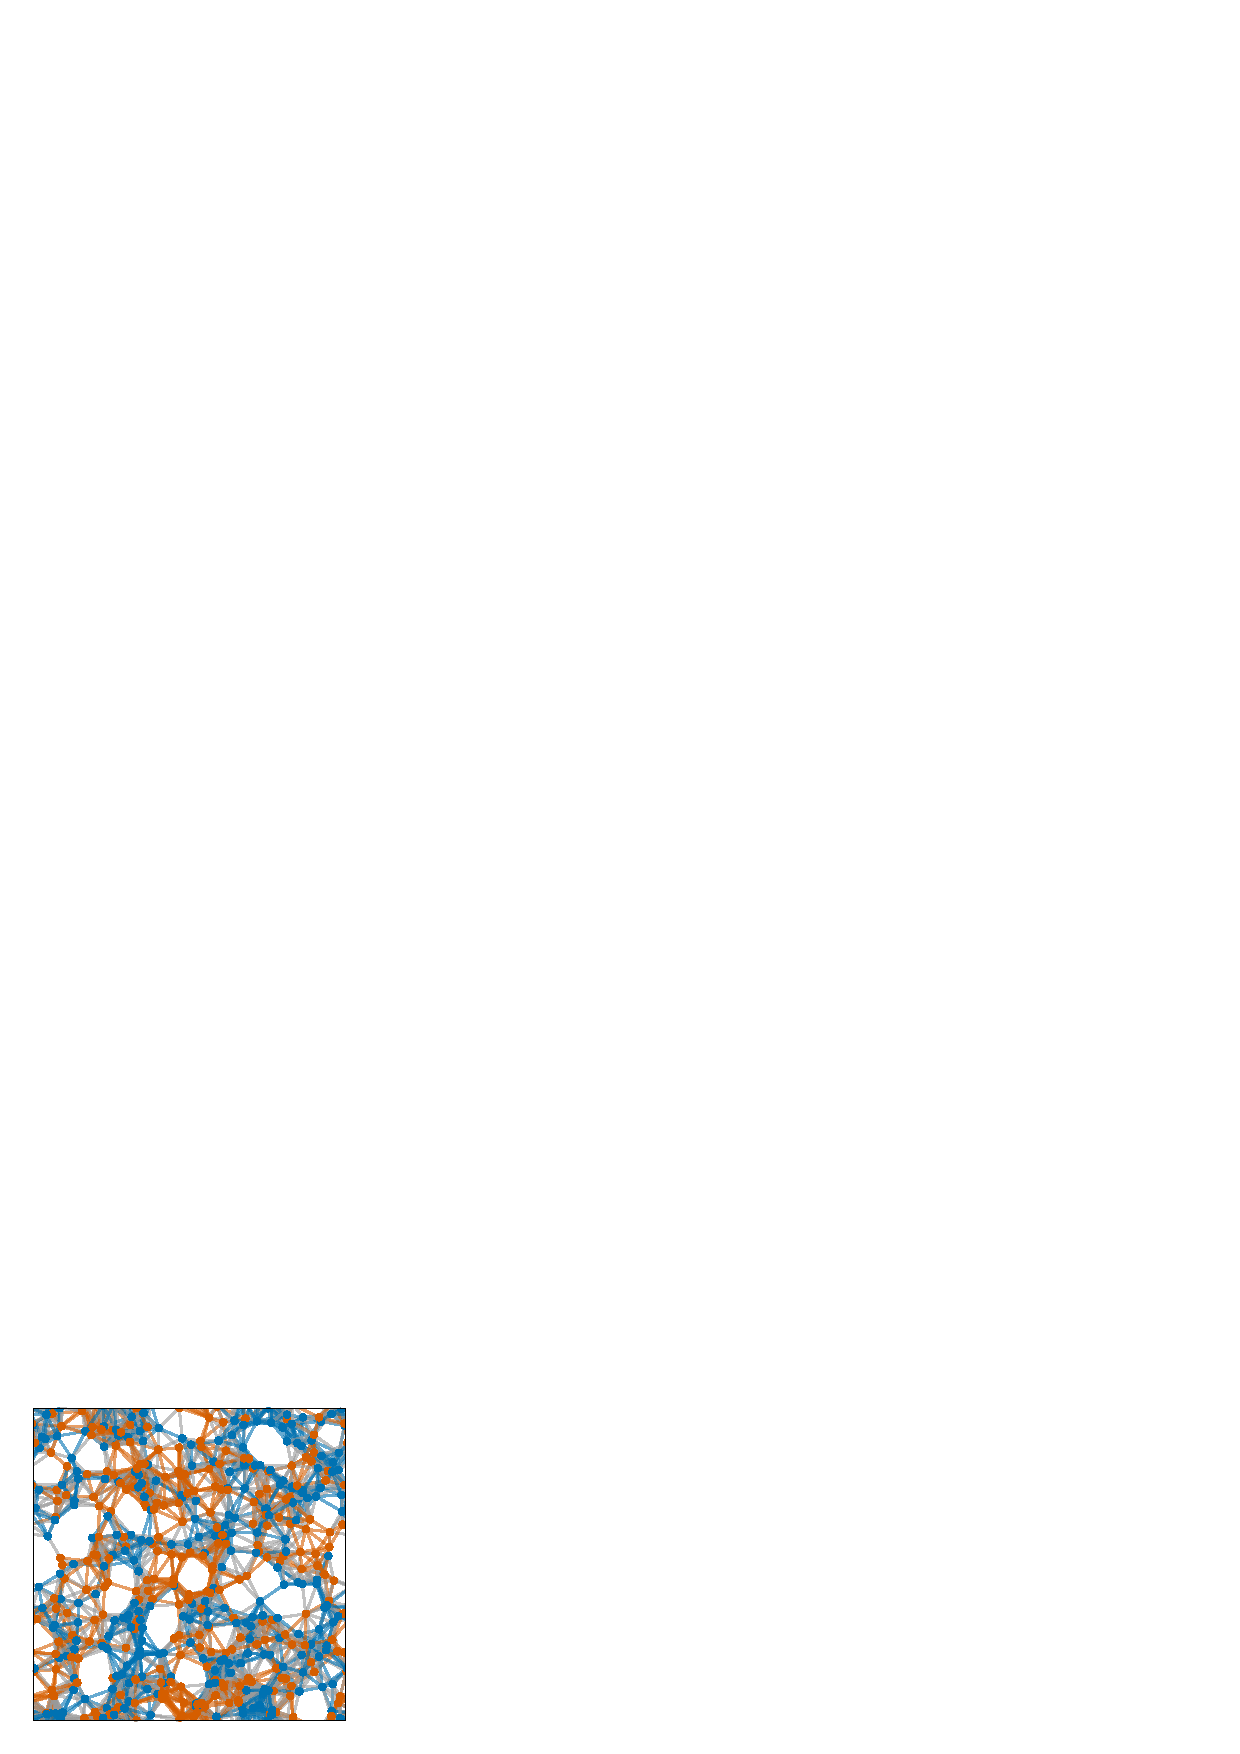
\includegraphics[page=1,width=0.132\textwidth]{../data/visualization}%
  \hspace{0.002\textwidth}%
  \includegraphics[page=2,width=0.132\textwidth]{../data/visualization}%
  \hspace{0.002\textwidth}%
  \includegraphics[page=3,width=0.132\textwidth]{../data/visualization}%
  \hspace{0.002\textwidth}%
  \includegraphics[page=4,width=0.132\textwidth]{../data/visualization}%
  \hspace{0.002\textwidth}%
  \includegraphics[page=5,width=0.132\textwidth]{../data/visualization}%
  \hspace{0.002\textwidth}%
  \includegraphics[page=6,width=0.132\textwidth]{../data/visualization}%
  \hspace{0.002\textwidth}%
  \includegraphics[page=7,width=0.132\textwidth]{../data/visualization}%
  
  % Created by tikzDevice version 0.12.3.1 on 2021-10-16 20:28:21
% !TEX encoding = UTF-8 Unicode
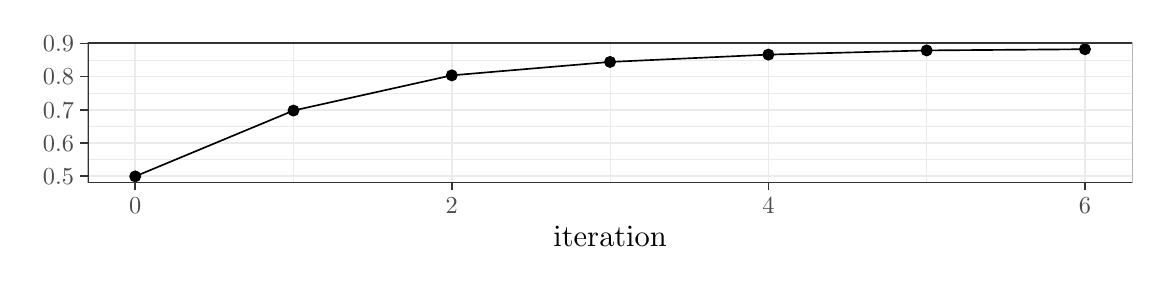
\begin{tikzpicture}[x=1pt,y=1pt]
\definecolor{fillColor}{RGB}{255,255,255}
\path[use as bounding box,fill=fillColor,fill opacity=0.00] (0,0) rectangle (404.71, 86.72);
\begin{scope}
\path[clip] (  0.00,  0.00) rectangle (404.71, 86.72);
\definecolor{drawColor}{RGB}{255,255,255}
\definecolor{fillColor}{RGB}{255,255,255}

\path[draw=drawColor,line width= 0.6pt,line join=round,line cap=round,fill=fillColor] (  0.00,  0.00) rectangle (404.71, 86.72);
\end{scope}
\begin{scope}
\path[clip] ( 21.69, 30.69) rectangle (399.21, 81.22);
\definecolor{fillColor}{RGB}{255,255,255}

\path[fill=fillColor] ( 21.69, 30.69) rectangle (399.21, 81.22);
\definecolor{drawColor}{gray}{0.92}

\path[draw=drawColor,line width= 0.3pt,line join=round] ( 21.69, 39.04) --
	(399.21, 39.04);

\path[draw=drawColor,line width= 0.3pt,line join=round] ( 21.69, 51.04) --
	(399.21, 51.04);

\path[draw=drawColor,line width= 0.3pt,line join=round] ( 21.69, 63.04) --
	(399.21, 63.04);

\path[draw=drawColor,line width= 0.3pt,line join=round] ( 21.69, 75.04) --
	(399.21, 75.04);

\path[draw=drawColor,line width= 0.3pt,line join=round] ( 96.05, 30.69) --
	( 96.05, 81.22);

\path[draw=drawColor,line width= 0.3pt,line join=round] (210.45, 30.69) --
	(210.45, 81.22);

\path[draw=drawColor,line width= 0.3pt,line join=round] (324.85, 30.69) --
	(324.85, 81.22);

\path[draw=drawColor,line width= 0.6pt,line join=round] ( 21.69, 33.04) --
	(399.21, 33.04);

\path[draw=drawColor,line width= 0.6pt,line join=round] ( 21.69, 45.04) --
	(399.21, 45.04);

\path[draw=drawColor,line width= 0.6pt,line join=round] ( 21.69, 57.04) --
	(399.21, 57.04);

\path[draw=drawColor,line width= 0.6pt,line join=round] ( 21.69, 69.04) --
	(399.21, 69.04);

\path[draw=drawColor,line width= 0.6pt,line join=round] ( 21.69, 81.04) --
	(399.21, 81.04);

\path[draw=drawColor,line width= 0.6pt,line join=round] ( 38.85, 30.69) --
	( 38.85, 81.22);

\path[draw=drawColor,line width= 0.6pt,line join=round] (153.25, 30.69) --
	(153.25, 81.22);

\path[draw=drawColor,line width= 0.6pt,line join=round] (267.65, 30.69) --
	(267.65, 81.22);

\path[draw=drawColor,line width= 0.6pt,line join=round] (382.05, 30.69) --
	(382.05, 81.22);
\definecolor{drawColor}{RGB}{0,0,0}

\path[draw=drawColor,line width= 0.6pt,line join=round] ( 38.85, 32.98) --
	( 96.05, 56.77) --
	(153.25, 69.49) --
	(210.45, 74.34) --
	(267.65, 76.98) --
	(324.85, 78.50) --
	(382.05, 78.93);
\definecolor{fillColor}{RGB}{0,0,0}

\path[draw=drawColor,line width= 0.4pt,line join=round,line cap=round,fill=fillColor] ( 38.85, 32.98) circle (  1.96);

\path[draw=drawColor,line width= 0.4pt,line join=round,line cap=round,fill=fillColor] ( 96.05, 56.77) circle (  1.96);

\path[draw=drawColor,line width= 0.4pt,line join=round,line cap=round,fill=fillColor] (153.25, 69.49) circle (  1.96);

\path[draw=drawColor,line width= 0.4pt,line join=round,line cap=round,fill=fillColor] (210.45, 74.34) circle (  1.96);

\path[draw=drawColor,line width= 0.4pt,line join=round,line cap=round,fill=fillColor] (267.65, 76.98) circle (  1.96);

\path[draw=drawColor,line width= 0.4pt,line join=round,line cap=round,fill=fillColor] (324.85, 78.50) circle (  1.96);

\path[draw=drawColor,line width= 0.4pt,line join=round,line cap=round,fill=fillColor] (382.05, 78.93) circle (  1.96);
\definecolor{drawColor}{gray}{0.20}

\path[draw=drawColor,line width= 0.6pt,line join=round,line cap=round] ( 21.69, 30.69) rectangle (399.21, 81.22);
\end{scope}
\begin{scope}
\path[clip] (  0.00,  0.00) rectangle (404.71, 86.72);
\definecolor{drawColor}{gray}{0.30}

\node[text=drawColor,anchor=base east,inner sep=0pt, outer sep=0pt, scale=  0.88] at ( 16.74, 30.01) {0.5};

\node[text=drawColor,anchor=base east,inner sep=0pt, outer sep=0pt, scale=  0.88] at ( 16.74, 42.01) {0.6};

\node[text=drawColor,anchor=base east,inner sep=0pt, outer sep=0pt, scale=  0.88] at ( 16.74, 54.01) {0.7};

\node[text=drawColor,anchor=base east,inner sep=0pt, outer sep=0pt, scale=  0.88] at ( 16.74, 66.01) {0.8};

\node[text=drawColor,anchor=base east,inner sep=0pt, outer sep=0pt, scale=  0.88] at ( 16.74, 78.01) {0.9};
\end{scope}
\begin{scope}
\path[clip] (  0.00,  0.00) rectangle (404.71, 86.72);
\definecolor{drawColor}{gray}{0.20}

\path[draw=drawColor,line width= 0.6pt,line join=round] ( 18.94, 33.04) --
	( 21.69, 33.04);

\path[draw=drawColor,line width= 0.6pt,line join=round] ( 18.94, 45.04) --
	( 21.69, 45.04);

\path[draw=drawColor,line width= 0.6pt,line join=round] ( 18.94, 57.04) --
	( 21.69, 57.04);

\path[draw=drawColor,line width= 0.6pt,line join=round] ( 18.94, 69.04) --
	( 21.69, 69.04);

\path[draw=drawColor,line width= 0.6pt,line join=round] ( 18.94, 81.04) --
	( 21.69, 81.04);
\end{scope}
\begin{scope}
\path[clip] (  0.00,  0.00) rectangle (404.71, 86.72);
\definecolor{drawColor}{gray}{0.20}

\path[draw=drawColor,line width= 0.6pt,line join=round] ( 38.85, 27.94) --
	( 38.85, 30.69);

\path[draw=drawColor,line width= 0.6pt,line join=round] (153.25, 27.94) --
	(153.25, 30.69);

\path[draw=drawColor,line width= 0.6pt,line join=round] (267.65, 27.94) --
	(267.65, 30.69);

\path[draw=drawColor,line width= 0.6pt,line join=round] (382.05, 27.94) --
	(382.05, 30.69);
\end{scope}
\begin{scope}
\path[clip] (  0.00,  0.00) rectangle (404.71, 86.72);
\definecolor{drawColor}{gray}{0.30}

\node[text=drawColor,anchor=base,inner sep=0pt, outer sep=0pt, scale=  0.88] at ( 38.85, 19.68) {0};

\node[text=drawColor,anchor=base,inner sep=0pt, outer sep=0pt, scale=  0.88] at (153.25, 19.68) {2};

\node[text=drawColor,anchor=base,inner sep=0pt, outer sep=0pt, scale=  0.88] at (267.65, 19.68) {4};

\node[text=drawColor,anchor=base,inner sep=0pt, outer sep=0pt, scale=  0.88] at (382.05, 19.68) {6};
\end{scope}
\begin{scope}
\path[clip] (  0.00,  0.00) rectangle (404.71, 86.72);
\definecolor{drawColor}{RGB}{0,0,0}

\node[text=drawColor,anchor=base,inner sep=0pt, outer sep=0pt, scale=  1.10] at (210.45,  7.64) {iteration};
\end{scope}
\end{tikzpicture}

  \caption{First six iterations for a graph with \num{500} vertices
    and average degree $16$ on the torus.  The $y$-axis of the bottom
    plot shows the fraction of monochrome edges.}
\end{figure}

\begin{figure}
  \centering
  \small
  % Created by tikzDevice version 0.12.3.1 on 2021-12-03 16:21:35
% !TEX encoding = UTF-8 Unicode
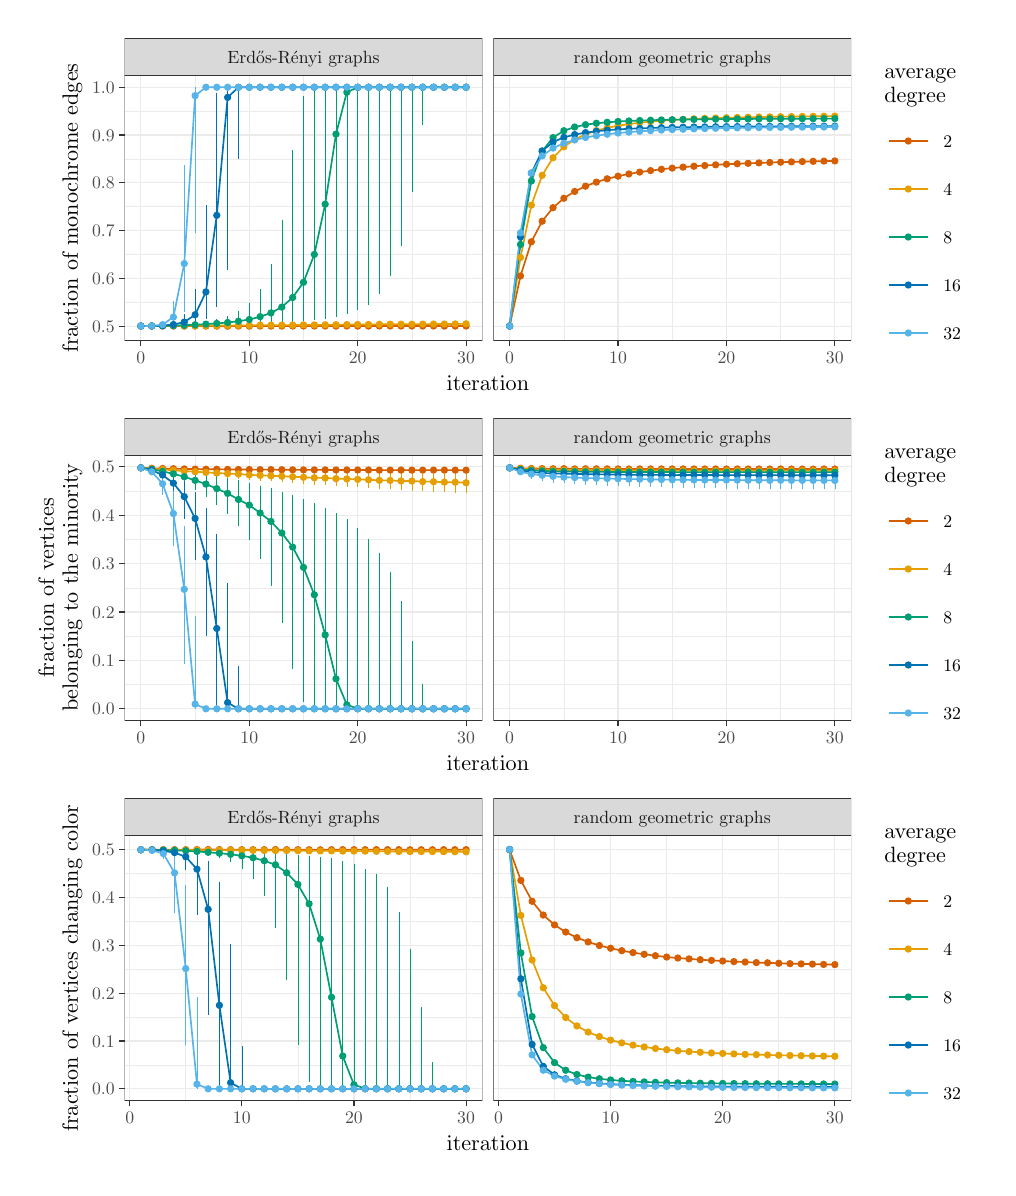
\begin{tikzpicture}[x=1pt,y=1pt]
\definecolor{fillColor}{RGB}{255,255,255}
\path[use as bounding box,fill=fillColor,fill opacity=0.00] (0,0) rectangle (346.90,411.94);
\begin{scope}
\path[clip] (  0.00,  0.00) rectangle (346.90,411.94);
\definecolor{drawColor}{gray}{0.30}

\node[text=drawColor,anchor=base east,inner sep=0pt, outer sep=0pt, scale=  0.64] at ( 31.44,301.91) {0.5};

\node[text=drawColor,anchor=base east,inner sep=0pt, outer sep=0pt, scale=  0.64] at ( 31.44,319.17) {0.6};

\node[text=drawColor,anchor=base east,inner sep=0pt, outer sep=0pt, scale=  0.64] at ( 31.44,336.43) {0.7};

\node[text=drawColor,anchor=base east,inner sep=0pt, outer sep=0pt, scale=  0.64] at ( 31.44,353.69) {0.8};

\node[text=drawColor,anchor=base east,inner sep=0pt, outer sep=0pt, scale=  0.64] at ( 31.44,370.95) {0.9};

\node[text=drawColor,anchor=base east,inner sep=0pt, outer sep=0pt, scale=  0.64] at ( 31.44,388.21) {1.0};
\end{scope}
\begin{scope}
\path[clip] (  0.00,  0.00) rectangle (346.90,411.94);
\definecolor{drawColor}{gray}{0.20}

\path[draw=drawColor,line width= 0.4pt,line join=round] ( 33.04,304.11) --
	( 35.04,304.11);

\path[draw=drawColor,line width= 0.4pt,line join=round] ( 33.04,321.37) --
	( 35.04,321.37);

\path[draw=drawColor,line width= 0.4pt,line join=round] ( 33.04,338.63) --
	( 35.04,338.63);

\path[draw=drawColor,line width= 0.4pt,line join=round] ( 33.04,355.89) --
	( 35.04,355.89);

\path[draw=drawColor,line width= 0.4pt,line join=round] ( 33.04,373.15) --
	( 35.04,373.15);

\path[draw=drawColor,line width= 0.4pt,line join=round] ( 33.04,390.41) --
	( 35.04,390.41);
\end{scope}
\begin{scope}
\path[clip] (  0.00,  0.00) rectangle (346.90,411.94);
\definecolor{drawColor}{RGB}{0,0,0}

\node[text=drawColor,rotate= 90.00,anchor=base,inner sep=0pt, outer sep=0pt, scale=  0.80] at ( 18.15,346.76) {fraction of monochrome edges};
\end{scope}
\begin{scope}
\path[clip] (  0.00,  0.00) rectangle (346.90,411.94);
\definecolor{drawColor}{gray}{0.30}

\node[text=drawColor,anchor=base east,inner sep=0pt, outer sep=0pt, scale=  0.64] at ( 31.44,163.60) {0.0};

\node[text=drawColor,anchor=base east,inner sep=0pt, outer sep=0pt, scale=  0.64] at ( 31.44,181.09) {0.1};

\node[text=drawColor,anchor=base east,inner sep=0pt, outer sep=0pt, scale=  0.64] at ( 31.44,198.59) {0.2};

\node[text=drawColor,anchor=base east,inner sep=0pt, outer sep=0pt, scale=  0.64] at ( 31.44,216.08) {0.3};

\node[text=drawColor,anchor=base east,inner sep=0pt, outer sep=0pt, scale=  0.64] at ( 31.44,233.57) {0.4};

\node[text=drawColor,anchor=base east,inner sep=0pt, outer sep=0pt, scale=  0.64] at ( 31.44,251.06) {0.5};
\end{scope}
\begin{scope}
\path[clip] (  0.00,  0.00) rectangle (346.90,411.94);
\definecolor{drawColor}{gray}{0.20}

\path[draw=drawColor,line width= 0.4pt,line join=round] ( 33.04,165.81) --
	( 35.04,165.81);

\path[draw=drawColor,line width= 0.4pt,line join=round] ( 33.04,183.30) --
	( 35.04,183.30);

\path[draw=drawColor,line width= 0.4pt,line join=round] ( 33.04,200.79) --
	( 35.04,200.79);

\path[draw=drawColor,line width= 0.4pt,line join=round] ( 33.04,218.28) --
	( 35.04,218.28);

\path[draw=drawColor,line width= 0.4pt,line join=round] ( 33.04,235.77) --
	( 35.04,235.77);

\path[draw=drawColor,line width= 0.4pt,line join=round] ( 33.04,253.26) --
	( 35.04,253.26);
\end{scope}
\begin{scope}
\path[clip] (  0.00,  0.00) rectangle (346.90,411.94);
\definecolor{drawColor}{RGB}{0,0,0}

\node[text=drawColor,rotate= 90.00,anchor=base,inner sep=0pt, outer sep=0pt, scale=  0.80] at (  9.51,209.45) {fraction of vertices};

\node[text=drawColor,rotate= 90.00,anchor=base,inner sep=0pt, outer sep=0pt, scale=  0.80] at ( 18.15,209.45) {belonging to the minority};
\end{scope}
\begin{scope}
\path[clip] (  0.00,  0.00) rectangle (346.90,411.94);
\definecolor{drawColor}{gray}{0.30}

\node[text=drawColor,anchor=base east,inner sep=0pt, outer sep=0pt, scale=  0.64] at ( 31.44, 26.29) {0.0};

\node[text=drawColor,anchor=base east,inner sep=0pt, outer sep=0pt, scale=  0.64] at ( 31.44, 43.58) {0.1};

\node[text=drawColor,anchor=base east,inner sep=0pt, outer sep=0pt, scale=  0.64] at ( 31.44, 60.86) {0.2};

\node[text=drawColor,anchor=base east,inner sep=0pt, outer sep=0pt, scale=  0.64] at ( 31.44, 78.15) {0.3};

\node[text=drawColor,anchor=base east,inner sep=0pt, outer sep=0pt, scale=  0.64] at ( 31.44, 95.43) {0.4};

\node[text=drawColor,anchor=base east,inner sep=0pt, outer sep=0pt, scale=  0.64] at ( 31.44,112.72) {0.5};
\end{scope}
\begin{scope}
\path[clip] (  0.00,  0.00) rectangle (346.90,411.94);
\definecolor{drawColor}{gray}{0.20}

\path[draw=drawColor,line width= 0.4pt,line join=round] ( 33.04, 28.49) --
	( 35.04, 28.49);

\path[draw=drawColor,line width= 0.4pt,line join=round] ( 33.04, 45.78) --
	( 35.04, 45.78);

\path[draw=drawColor,line width= 0.4pt,line join=round] ( 33.04, 63.07) --
	( 35.04, 63.07);

\path[draw=drawColor,line width= 0.4pt,line join=round] ( 33.04, 80.35) --
	( 35.04, 80.35);

\path[draw=drawColor,line width= 0.4pt,line join=round] ( 33.04, 97.64) --
	( 35.04, 97.64);

\path[draw=drawColor,line width= 0.4pt,line join=round] ( 33.04,114.92) --
	( 35.04,114.92);
\end{scope}
\begin{scope}
\path[clip] (  0.00,  0.00) rectangle (346.90,411.94);
\definecolor{drawColor}{RGB}{0,0,0}

\node[text=drawColor,rotate= 90.00,anchor=base,inner sep=0pt, outer sep=0pt, scale=  0.80] at ( 18.15, 72.14) {fraction of vertices changing color};
\end{scope}
\begin{scope}
\path[clip] ( 35.04,394.77) rectangle (164.29,407.94);
\definecolor{drawColor}{gray}{0.20}
\definecolor{fillColor}{gray}{0.85}

\path[draw=drawColor,line width= 0.4pt,line join=round,line cap=round,fill=fillColor] ( 35.04,394.77) rectangle (164.29,407.94);
\definecolor{drawColor}{gray}{0.10}

\node[text=drawColor,anchor=base,inner sep=0pt, outer sep=0pt, scale=  0.64] at ( 99.66,399.15) {Erd{\H o}s-R\'enyi graphs};
\end{scope}
\begin{scope}
\path[clip] (168.29,394.77) rectangle (297.54,407.94);
\definecolor{drawColor}{gray}{0.20}
\definecolor{fillColor}{gray}{0.85}

\path[draw=drawColor,line width= 0.4pt,line join=round,line cap=round,fill=fillColor] (168.29,394.77) rectangle (297.54,407.94);
\definecolor{drawColor}{gray}{0.10}

\node[text=drawColor,anchor=base,inner sep=0pt, outer sep=0pt, scale=  0.64] at (232.91,399.15) {random geometric graphs};
\end{scope}
\begin{scope}
\path[clip] ( 35.04,257.46) rectangle (164.29,270.63);
\definecolor{drawColor}{gray}{0.20}
\definecolor{fillColor}{gray}{0.85}

\path[draw=drawColor,line width= 0.4pt,line join=round,line cap=round,fill=fillColor] ( 35.04,257.46) rectangle (164.29,270.63);
\definecolor{drawColor}{gray}{0.10}

\node[text=drawColor,anchor=base,inner sep=0pt, outer sep=0pt, scale=  0.64] at ( 99.66,261.84) {Erd{\H o}s-R\'enyi graphs};
\end{scope}
\begin{scope}
\path[clip] (168.29,257.46) rectangle (297.54,270.63);
\definecolor{drawColor}{gray}{0.20}
\definecolor{fillColor}{gray}{0.85}

\path[draw=drawColor,line width= 0.4pt,line join=round,line cap=round,fill=fillColor] (168.29,257.46) rectangle (297.54,270.63);
\definecolor{drawColor}{gray}{0.10}

\node[text=drawColor,anchor=base,inner sep=0pt, outer sep=0pt, scale=  0.64] at (232.91,261.84) {random geometric graphs};
\end{scope}
\begin{scope}
\path[clip] ( 35.04,120.15) rectangle (164.29,133.31);
\definecolor{drawColor}{gray}{0.20}
\definecolor{fillColor}{gray}{0.85}

\path[draw=drawColor,line width= 0.4pt,line join=round,line cap=round,fill=fillColor] ( 35.04,120.15) rectangle (164.29,133.31);
\definecolor{drawColor}{gray}{0.10}

\node[text=drawColor,anchor=base,inner sep=0pt, outer sep=0pt, scale=  0.64] at ( 99.66,124.53) {Erd{\H o}s-R\'enyi graphs};
\end{scope}
\begin{scope}
\path[clip] (168.29,120.15) rectangle (297.54,133.31);
\definecolor{drawColor}{gray}{0.20}
\definecolor{fillColor}{gray}{0.85}

\path[draw=drawColor,line width= 0.4pt,line join=round,line cap=round,fill=fillColor] (168.29,120.15) rectangle (297.54,133.31);
\definecolor{drawColor}{gray}{0.10}

\node[text=drawColor,anchor=base,inner sep=0pt, outer sep=0pt, scale=  0.64] at (232.91,124.53) {random geometric graphs};
\end{scope}
\begin{scope}
\path[clip] ( 35.04,298.76) rectangle (164.29,394.77);
\definecolor{fillColor}{RGB}{255,255,255}

\path[fill=fillColor] ( 35.04,298.76) rectangle (164.29,394.77);
\definecolor{drawColor}{gray}{0.92}

\path[draw=drawColor,line width= 0.2pt,line join=round] ( 35.04,312.74) --
	(164.29,312.74);

\path[draw=drawColor,line width= 0.2pt,line join=round] ( 35.04,330.00) --
	(164.29,330.00);

\path[draw=drawColor,line width= 0.2pt,line join=round] ( 35.04,347.26) --
	(164.29,347.26);

\path[draw=drawColor,line width= 0.2pt,line join=round] ( 35.04,364.52) --
	(164.29,364.52);

\path[draw=drawColor,line width= 0.2pt,line join=round] ( 35.04,381.78) --
	(164.29,381.78);

\path[draw=drawColor,line width= 0.2pt,line join=round] ( 60.50,298.76) --
	( 60.50,394.77);

\path[draw=drawColor,line width= 0.2pt,line join=round] ( 99.66,298.76) --
	( 99.66,394.77);

\path[draw=drawColor,line width= 0.2pt,line join=round] (138.83,298.76) --
	(138.83,394.77);

\path[draw=drawColor,line width= 0.4pt,line join=round] ( 35.04,304.11) --
	(164.29,304.11);

\path[draw=drawColor,line width= 0.4pt,line join=round] ( 35.04,321.37) --
	(164.29,321.37);

\path[draw=drawColor,line width= 0.4pt,line join=round] ( 35.04,338.63) --
	(164.29,338.63);

\path[draw=drawColor,line width= 0.4pt,line join=round] ( 35.04,355.89) --
	(164.29,355.89);

\path[draw=drawColor,line width= 0.4pt,line join=round] ( 35.04,373.15) --
	(164.29,373.15);

\path[draw=drawColor,line width= 0.4pt,line join=round] ( 35.04,390.41) --
	(164.29,390.41);

\path[draw=drawColor,line width= 0.4pt,line join=round] ( 40.91,298.76) --
	( 40.91,394.77);

\path[draw=drawColor,line width= 0.4pt,line join=round] ( 80.08,298.76) --
	( 80.08,394.77);

\path[draw=drawColor,line width= 0.4pt,line join=round] (119.25,298.76) --
	(119.25,394.77);

\path[draw=drawColor,line width= 0.4pt,line join=round] (158.41,298.76) --
	(158.41,394.77);
\definecolor{drawColor}{RGB}{213,94,0}

\path[draw=drawColor,line width= 0.2pt,line join=round] ( 40.91,304.48) --
	( 40.91,304.48);

\path[draw=drawColor,line width= 0.2pt,line join=round] ( 40.91,304.48) --
	( 40.91,303.74);

\path[draw=drawColor,line width= 0.2pt,line join=round] ( 40.91,303.74) --
	( 40.91,303.74);

\path[draw=drawColor,line width= 0.2pt,line join=round] ( 44.83,304.74) --
	( 44.83,304.74);

\path[draw=drawColor,line width= 0.2pt,line join=round] ( 44.83,304.74) --
	( 44.83,303.53);

\path[draw=drawColor,line width= 0.2pt,line join=round] ( 44.83,303.53) --
	( 44.83,303.53);

\path[draw=drawColor,line width= 0.2pt,line join=round] ( 48.75,304.81) --
	( 48.75,304.81);

\path[draw=drawColor,line width= 0.2pt,line join=round] ( 48.75,304.81) --
	( 48.75,303.49);

\path[draw=drawColor,line width= 0.2pt,line join=round] ( 48.75,303.49) --
	( 48.75,303.49);

\path[draw=drawColor,line width= 0.2pt,line join=round] ( 52.66,304.84) --
	( 52.66,304.84);

\path[draw=drawColor,line width= 0.2pt,line join=round] ( 52.66,304.84) --
	( 52.66,303.45);

\path[draw=drawColor,line width= 0.2pt,line join=round] ( 52.66,303.45) --
	( 52.66,303.45);

\path[draw=drawColor,line width= 0.2pt,line join=round] ( 56.58,304.84) --
	( 56.58,304.84);

\path[draw=drawColor,line width= 0.2pt,line join=round] ( 56.58,304.84) --
	( 56.58,303.39);

\path[draw=drawColor,line width= 0.2pt,line join=round] ( 56.58,303.39) --
	( 56.58,303.39);

\path[draw=drawColor,line width= 0.2pt,line join=round] ( 60.50,304.84) --
	( 60.50,304.84);

\path[draw=drawColor,line width= 0.2pt,line join=round] ( 60.50,304.84) --
	( 60.50,303.41);

\path[draw=drawColor,line width= 0.2pt,line join=round] ( 60.50,303.41) --
	( 60.50,303.41);

\path[draw=drawColor,line width= 0.2pt,line join=round] ( 64.41,304.87) --
	( 64.41,304.87);

\path[draw=drawColor,line width= 0.2pt,line join=round] ( 64.41,304.87) --
	( 64.41,303.33);

\path[draw=drawColor,line width= 0.2pt,line join=round] ( 64.41,303.33) --
	( 64.41,303.33);

\path[draw=drawColor,line width= 0.2pt,line join=round] ( 68.33,304.88) --
	( 68.33,304.88);

\path[draw=drawColor,line width= 0.2pt,line join=round] ( 68.33,304.88) --
	( 68.33,303.28);

\path[draw=drawColor,line width= 0.2pt,line join=round] ( 68.33,303.28) --
	( 68.33,303.28);

\path[draw=drawColor,line width= 0.2pt,line join=round] ( 72.25,304.93) --
	( 72.25,304.93);

\path[draw=drawColor,line width= 0.2pt,line join=round] ( 72.25,304.93) --
	( 72.25,303.25);

\path[draw=drawColor,line width= 0.2pt,line join=round] ( 72.25,303.25) --
	( 72.25,303.25);

\path[draw=drawColor,line width= 0.2pt,line join=round] ( 76.16,304.96) --
	( 76.16,304.96);

\path[draw=drawColor,line width= 0.2pt,line join=round] ( 76.16,304.96) --
	( 76.16,303.20);

\path[draw=drawColor,line width= 0.2pt,line join=round] ( 76.16,303.20) --
	( 76.16,303.20);

\path[draw=drawColor,line width= 0.2pt,line join=round] ( 80.08,304.95) --
	( 80.08,304.95);

\path[draw=drawColor,line width= 0.2pt,line join=round] ( 80.08,304.95) --
	( 80.08,303.17);

\path[draw=drawColor,line width= 0.2pt,line join=round] ( 80.08,303.17) --
	( 80.08,303.17);

\path[draw=drawColor,line width= 0.2pt,line join=round] ( 84.00,304.98) --
	( 84.00,304.98);

\path[draw=drawColor,line width= 0.2pt,line join=round] ( 84.00,304.98) --
	( 84.00,303.24);

\path[draw=drawColor,line width= 0.2pt,line join=round] ( 84.00,303.24) --
	( 84.00,303.24);

\path[draw=drawColor,line width= 0.2pt,line join=round] ( 87.91,305.01) --
	( 87.91,305.01);

\path[draw=drawColor,line width= 0.2pt,line join=round] ( 87.91,305.01) --
	( 87.91,303.19);

\path[draw=drawColor,line width= 0.2pt,line join=round] ( 87.91,303.19) --
	( 87.91,303.19);

\path[draw=drawColor,line width= 0.2pt,line join=round] ( 91.83,305.02) --
	( 91.83,305.02);

\path[draw=drawColor,line width= 0.2pt,line join=round] ( 91.83,305.02) --
	( 91.83,303.25);

\path[draw=drawColor,line width= 0.2pt,line join=round] ( 91.83,303.25) --
	( 91.83,303.25);

\path[draw=drawColor,line width= 0.2pt,line join=round] ( 95.75,305.05) --
	( 95.75,305.05);

\path[draw=drawColor,line width= 0.2pt,line join=round] ( 95.75,305.05) --
	( 95.75,303.22);

\path[draw=drawColor,line width= 0.2pt,line join=round] ( 95.75,303.22) --
	( 95.75,303.22);

\path[draw=drawColor,line width= 0.2pt,line join=round] ( 99.66,305.07) --
	( 99.66,305.07);

\path[draw=drawColor,line width= 0.2pt,line join=round] ( 99.66,305.07) --
	( 99.66,303.20);

\path[draw=drawColor,line width= 0.2pt,line join=round] ( 99.66,303.20) --
	( 99.66,303.20);

\path[draw=drawColor,line width= 0.2pt,line join=round] (103.58,305.07) --
	(103.58,305.07);

\path[draw=drawColor,line width= 0.2pt,line join=round] (103.58,305.07) --
	(103.58,303.20);

\path[draw=drawColor,line width= 0.2pt,line join=round] (103.58,303.20) --
	(103.58,303.20);

\path[draw=drawColor,line width= 0.2pt,line join=round] (107.50,305.06) --
	(107.50,305.06);

\path[draw=drawColor,line width= 0.2pt,line join=round] (107.50,305.06) --
	(107.50,303.22);

\path[draw=drawColor,line width= 0.2pt,line join=round] (107.50,303.22) --
	(107.50,303.22);

\path[draw=drawColor,line width= 0.2pt,line join=round] (111.41,305.10) --
	(111.41,305.10);

\path[draw=drawColor,line width= 0.2pt,line join=round] (111.41,305.10) --
	(111.41,303.17);

\path[draw=drawColor,line width= 0.2pt,line join=round] (111.41,303.17) --
	(111.41,303.17);

\path[draw=drawColor,line width= 0.2pt,line join=round] (115.33,305.07) --
	(115.33,305.07);

\path[draw=drawColor,line width= 0.2pt,line join=round] (115.33,305.07) --
	(115.33,303.21);

\path[draw=drawColor,line width= 0.2pt,line join=round] (115.33,303.21) --
	(115.33,303.21);

\path[draw=drawColor,line width= 0.2pt,line join=round] (119.25,305.08) --
	(119.25,305.08);

\path[draw=drawColor,line width= 0.2pt,line join=round] (119.25,305.08) --
	(119.25,303.21);

\path[draw=drawColor,line width= 0.2pt,line join=round] (119.25,303.21) --
	(119.25,303.21);

\path[draw=drawColor,line width= 0.2pt,line join=round] (123.16,305.11) --
	(123.16,305.11);

\path[draw=drawColor,line width= 0.2pt,line join=round] (123.16,305.11) --
	(123.16,303.17);

\path[draw=drawColor,line width= 0.2pt,line join=round] (123.16,303.17) --
	(123.16,303.17);

\path[draw=drawColor,line width= 0.2pt,line join=round] (127.08,305.11) --
	(127.08,305.11);

\path[draw=drawColor,line width= 0.2pt,line join=round] (127.08,305.11) --
	(127.08,303.20);

\path[draw=drawColor,line width= 0.2pt,line join=round] (127.08,303.20) --
	(127.08,303.20);

\path[draw=drawColor,line width= 0.2pt,line join=round] (131.00,305.07) --
	(131.00,305.07);

\path[draw=drawColor,line width= 0.2pt,line join=round] (131.00,305.07) --
	(131.00,303.17);

\path[draw=drawColor,line width= 0.2pt,line join=round] (131.00,303.17) --
	(131.00,303.17);

\path[draw=drawColor,line width= 0.2pt,line join=round] (134.91,305.12) --
	(134.91,305.12);

\path[draw=drawColor,line width= 0.2pt,line join=round] (134.91,305.12) --
	(134.91,303.21);

\path[draw=drawColor,line width= 0.2pt,line join=round] (134.91,303.21) --
	(134.91,303.21);

\path[draw=drawColor,line width= 0.2pt,line join=round] (138.83,305.08) --
	(138.83,305.08);

\path[draw=drawColor,line width= 0.2pt,line join=round] (138.83,305.08) --
	(138.83,303.14);

\path[draw=drawColor,line width= 0.2pt,line join=round] (138.83,303.14) --
	(138.83,303.14);

\path[draw=drawColor,line width= 0.2pt,line join=round] (142.75,305.09) --
	(142.75,305.09);

\path[draw=drawColor,line width= 0.2pt,line join=round] (142.75,305.09) --
	(142.75,303.17);

\path[draw=drawColor,line width= 0.2pt,line join=round] (142.75,303.17) --
	(142.75,303.17);

\path[draw=drawColor,line width= 0.2pt,line join=round] (146.66,305.08) --
	(146.66,305.08);

\path[draw=drawColor,line width= 0.2pt,line join=round] (146.66,305.08) --
	(146.66,303.13);

\path[draw=drawColor,line width= 0.2pt,line join=round] (146.66,303.13) --
	(146.66,303.13);

\path[draw=drawColor,line width= 0.2pt,line join=round] (150.58,305.09) --
	(150.58,305.09);

\path[draw=drawColor,line width= 0.2pt,line join=round] (150.58,305.09) --
	(150.58,303.14);

\path[draw=drawColor,line width= 0.2pt,line join=round] (150.58,303.14) --
	(150.58,303.14);

\path[draw=drawColor,line width= 0.2pt,line join=round] (154.50,305.09) --
	(154.50,305.09);

\path[draw=drawColor,line width= 0.2pt,line join=round] (154.50,305.09) --
	(154.50,303.18);

\path[draw=drawColor,line width= 0.2pt,line join=round] (154.50,303.18) --
	(154.50,303.18);

\path[draw=drawColor,line width= 0.2pt,line join=round] (158.41,305.10) --
	(158.41,305.10);

\path[draw=drawColor,line width= 0.2pt,line join=round] (158.41,305.10) --
	(158.41,303.12);

\path[draw=drawColor,line width= 0.2pt,line join=round] (158.41,303.12) --
	(158.41,303.12);
\definecolor{drawColor}{RGB}{230,159,0}

\path[draw=drawColor,line width= 0.2pt,line join=round] ( 40.91,304.40) --
	( 40.91,304.40);

\path[draw=drawColor,line width= 0.2pt,line join=round] ( 40.91,304.40) --
	( 40.91,303.89);

\path[draw=drawColor,line width= 0.2pt,line join=round] ( 40.91,303.89) --
	( 40.91,303.89);

\path[draw=drawColor,line width= 0.2pt,line join=round] ( 44.83,304.58) --
	( 44.83,304.58);

\path[draw=drawColor,line width= 0.2pt,line join=round] ( 44.83,304.58) --
	( 44.83,303.74);

\path[draw=drawColor,line width= 0.2pt,line join=round] ( 44.83,303.74) --
	( 44.83,303.74);

\path[draw=drawColor,line width= 0.2pt,line join=round] ( 48.75,304.68) --
	( 48.75,304.68);

\path[draw=drawColor,line width= 0.2pt,line join=round] ( 48.75,304.68) --
	( 48.75,303.67);

\path[draw=drawColor,line width= 0.2pt,line join=round] ( 48.75,303.67) --
	( 48.75,303.67);

\path[draw=drawColor,line width= 0.2pt,line join=round] ( 52.66,304.78) --
	( 52.66,304.78);

\path[draw=drawColor,line width= 0.2pt,line join=round] ( 52.66,304.78) --
	( 52.66,303.62);

\path[draw=drawColor,line width= 0.2pt,line join=round] ( 52.66,303.62) --
	( 52.66,303.62);

\path[draw=drawColor,line width= 0.2pt,line join=round] ( 56.58,304.87) --
	( 56.58,304.87);

\path[draw=drawColor,line width= 0.2pt,line join=round] ( 56.58,304.87) --
	( 56.58,303.56);

\path[draw=drawColor,line width= 0.2pt,line join=round] ( 56.58,303.56) --
	( 56.58,303.56);

\path[draw=drawColor,line width= 0.2pt,line join=round] ( 60.50,304.90) --
	( 60.50,304.90);

\path[draw=drawColor,line width= 0.2pt,line join=round] ( 60.50,304.90) --
	( 60.50,303.55);

\path[draw=drawColor,line width= 0.2pt,line join=round] ( 60.50,303.55) --
	( 60.50,303.55);

\path[draw=drawColor,line width= 0.2pt,line join=round] ( 64.41,304.97) --
	( 64.41,304.97);

\path[draw=drawColor,line width= 0.2pt,line join=round] ( 64.41,304.97) --
	( 64.41,303.53);

\path[draw=drawColor,line width= 0.2pt,line join=round] ( 64.41,303.53) --
	( 64.41,303.53);

\path[draw=drawColor,line width= 0.2pt,line join=round] ( 68.33,304.97) --
	( 68.33,304.97);

\path[draw=drawColor,line width= 0.2pt,line join=round] ( 68.33,304.97) --
	( 68.33,303.54);

\path[draw=drawColor,line width= 0.2pt,line join=round] ( 68.33,303.54) --
	( 68.33,303.54);

\path[draw=drawColor,line width= 0.2pt,line join=round] ( 72.25,305.02) --
	( 72.25,305.02);

\path[draw=drawColor,line width= 0.2pt,line join=round] ( 72.25,305.02) --
	( 72.25,303.56);

\path[draw=drawColor,line width= 0.2pt,line join=round] ( 72.25,303.56) --
	( 72.25,303.56);

\path[draw=drawColor,line width= 0.2pt,line join=round] ( 76.16,305.07) --
	( 76.16,305.07);

\path[draw=drawColor,line width= 0.2pt,line join=round] ( 76.16,305.07) --
	( 76.16,303.59);

\path[draw=drawColor,line width= 0.2pt,line join=round] ( 76.16,303.59) --
	( 76.16,303.59);

\path[draw=drawColor,line width= 0.2pt,line join=round] ( 80.08,305.16) --
	( 80.08,305.16);

\path[draw=drawColor,line width= 0.2pt,line join=round] ( 80.08,305.16) --
	( 80.08,303.55);

\path[draw=drawColor,line width= 0.2pt,line join=round] ( 80.08,303.55) --
	( 80.08,303.55);

\path[draw=drawColor,line width= 0.2pt,line join=round] ( 84.00,305.26) --
	( 84.00,305.26);

\path[draw=drawColor,line width= 0.2pt,line join=round] ( 84.00,305.26) --
	( 84.00,303.60);

\path[draw=drawColor,line width= 0.2pt,line join=round] ( 84.00,303.60) --
	( 84.00,303.60);

\path[draw=drawColor,line width= 0.2pt,line join=round] ( 87.91,305.28) --
	( 87.91,305.28);

\path[draw=drawColor,line width= 0.2pt,line join=round] ( 87.91,305.28) --
	( 87.91,303.59);

\path[draw=drawColor,line width= 0.2pt,line join=round] ( 87.91,303.59) --
	( 87.91,303.59);

\path[draw=drawColor,line width= 0.2pt,line join=round] ( 91.83,305.27) --
	( 91.83,305.27);

\path[draw=drawColor,line width= 0.2pt,line join=round] ( 91.83,305.27) --
	( 91.83,303.64);

\path[draw=drawColor,line width= 0.2pt,line join=round] ( 91.83,303.64) --
	( 91.83,303.64);

\path[draw=drawColor,line width= 0.2pt,line join=round] ( 95.75,305.33) --
	( 95.75,305.33);

\path[draw=drawColor,line width= 0.2pt,line join=round] ( 95.75,305.33) --
	( 95.75,303.58);

\path[draw=drawColor,line width= 0.2pt,line join=round] ( 95.75,303.58) --
	( 95.75,303.58);

\path[draw=drawColor,line width= 0.2pt,line join=round] ( 99.66,305.42) --
	( 99.66,305.42);

\path[draw=drawColor,line width= 0.2pt,line join=round] ( 99.66,305.42) --
	( 99.66,303.66);

\path[draw=drawColor,line width= 0.2pt,line join=round] ( 99.66,303.66) --
	( 99.66,303.66);

\path[draw=drawColor,line width= 0.2pt,line join=round] (103.58,305.43) --
	(103.58,305.43);

\path[draw=drawColor,line width= 0.2pt,line join=round] (103.58,305.43) --
	(103.58,303.62);

\path[draw=drawColor,line width= 0.2pt,line join=round] (103.58,303.62) --
	(103.58,303.62);

\path[draw=drawColor,line width= 0.2pt,line join=round] (107.50,305.44) --
	(107.50,305.44);

\path[draw=drawColor,line width= 0.2pt,line join=round] (107.50,305.44) --
	(107.50,303.71);

\path[draw=drawColor,line width= 0.2pt,line join=round] (107.50,303.71) --
	(107.50,303.71);

\path[draw=drawColor,line width= 0.2pt,line join=round] (111.41,305.58) --
	(111.41,305.58);

\path[draw=drawColor,line width= 0.2pt,line join=round] (111.41,305.58) --
	(111.41,303.69);

\path[draw=drawColor,line width= 0.2pt,line join=round] (111.41,303.69) --
	(111.41,303.69);

\path[draw=drawColor,line width= 0.2pt,line join=round] (115.33,305.62) --
	(115.33,305.62);

\path[draw=drawColor,line width= 0.2pt,line join=round] (115.33,305.62) --
	(115.33,303.74);

\path[draw=drawColor,line width= 0.2pt,line join=round] (115.33,303.74) --
	(115.33,303.74);

\path[draw=drawColor,line width= 0.2pt,line join=round] (119.25,305.63) --
	(119.25,305.63);

\path[draw=drawColor,line width= 0.2pt,line join=round] (119.25,305.63) --
	(119.25,303.66);

\path[draw=drawColor,line width= 0.2pt,line join=round] (119.25,303.66) --
	(119.25,303.66);

\path[draw=drawColor,line width= 0.2pt,line join=round] (123.16,305.66) --
	(123.16,305.66);

\path[draw=drawColor,line width= 0.2pt,line join=round] (123.16,305.66) --
	(123.16,303.74);

\path[draw=drawColor,line width= 0.2pt,line join=round] (123.16,303.74) --
	(123.16,303.74);

\path[draw=drawColor,line width= 0.2pt,line join=round] (127.08,305.71) --
	(127.08,305.71);

\path[draw=drawColor,line width= 0.2pt,line join=round] (127.08,305.71) --
	(127.08,303.75);

\path[draw=drawColor,line width= 0.2pt,line join=round] (127.08,303.75) --
	(127.08,303.75);

\path[draw=drawColor,line width= 0.2pt,line join=round] (131.00,305.79) --
	(131.00,305.79);

\path[draw=drawColor,line width= 0.2pt,line join=round] (131.00,305.79) --
	(131.00,303.78);

\path[draw=drawColor,line width= 0.2pt,line join=round] (131.00,303.78) --
	(131.00,303.78);

\path[draw=drawColor,line width= 0.2pt,line join=round] (134.91,305.84) --
	(134.91,305.84);

\path[draw=drawColor,line width= 0.2pt,line join=round] (134.91,305.84) --
	(134.91,303.77);

\path[draw=drawColor,line width= 0.2pt,line join=round] (134.91,303.77) --
	(134.91,303.77);

\path[draw=drawColor,line width= 0.2pt,line join=round] (138.83,305.85) --
	(138.83,305.85);

\path[draw=drawColor,line width= 0.2pt,line join=round] (138.83,305.85) --
	(138.83,303.82);

\path[draw=drawColor,line width= 0.2pt,line join=round] (138.83,303.82) --
	(138.83,303.82);

\path[draw=drawColor,line width= 0.2pt,line join=round] (142.75,305.89) --
	(142.75,305.89);

\path[draw=drawColor,line width= 0.2pt,line join=round] (142.75,305.89) --
	(142.75,303.78);

\path[draw=drawColor,line width= 0.2pt,line join=round] (142.75,303.78) --
	(142.75,303.78);

\path[draw=drawColor,line width= 0.2pt,line join=round] (146.66,305.94) --
	(146.66,305.94);

\path[draw=drawColor,line width= 0.2pt,line join=round] (146.66,305.94) --
	(146.66,303.78);

\path[draw=drawColor,line width= 0.2pt,line join=round] (146.66,303.78) --
	(146.66,303.78);

\path[draw=drawColor,line width= 0.2pt,line join=round] (150.58,305.94) --
	(150.58,305.94);

\path[draw=drawColor,line width= 0.2pt,line join=round] (150.58,305.94) --
	(150.58,303.82);

\path[draw=drawColor,line width= 0.2pt,line join=round] (150.58,303.82) --
	(150.58,303.82);

\path[draw=drawColor,line width= 0.2pt,line join=round] (154.50,305.97) --
	(154.50,305.97);

\path[draw=drawColor,line width= 0.2pt,line join=round] (154.50,305.97) --
	(154.50,303.84);

\path[draw=drawColor,line width= 0.2pt,line join=round] (154.50,303.84) --
	(154.50,303.84);

\path[draw=drawColor,line width= 0.2pt,line join=round] (158.41,306.00) --
	(158.41,306.00);

\path[draw=drawColor,line width= 0.2pt,line join=round] (158.41,306.00) --
	(158.41,303.88);

\path[draw=drawColor,line width= 0.2pt,line join=round] (158.41,303.88) --
	(158.41,303.88);
\definecolor{drawColor}{RGB}{0,158,115}

\path[draw=drawColor,line width= 0.2pt,line join=round] ( 40.91,304.30) --
	( 40.91,304.30);

\path[draw=drawColor,line width= 0.2pt,line join=round] ( 40.91,304.30) --
	( 40.91,303.92);

\path[draw=drawColor,line width= 0.2pt,line join=round] ( 40.91,303.92) --
	( 40.91,303.92);

\path[draw=drawColor,line width= 0.2pt,line join=round] ( 44.83,304.43) --
	( 44.83,304.43);

\path[draw=drawColor,line width= 0.2pt,line join=round] ( 44.83,304.43) --
	( 44.83,303.82);

\path[draw=drawColor,line width= 0.2pt,line join=round] ( 44.83,303.82) --
	( 44.83,303.82);

\path[draw=drawColor,line width= 0.2pt,line join=round] ( 48.75,304.56) --
	( 48.75,304.56);

\path[draw=drawColor,line width= 0.2pt,line join=round] ( 48.75,304.56) --
	( 48.75,303.83);

\path[draw=drawColor,line width= 0.2pt,line join=round] ( 48.75,303.83) --
	( 48.75,303.83);

\path[draw=drawColor,line width= 0.2pt,line join=round] ( 52.66,304.76) --
	( 52.66,304.76);

\path[draw=drawColor,line width= 0.2pt,line join=round] ( 52.66,304.76) --
	( 52.66,303.83);

\path[draw=drawColor,line width= 0.2pt,line join=round] ( 52.66,303.83) --
	( 52.66,303.83);

\path[draw=drawColor,line width= 0.2pt,line join=round] ( 56.58,304.98) --
	( 56.58,304.98);

\path[draw=drawColor,line width= 0.2pt,line join=round] ( 56.58,304.98) --
	( 56.58,303.92);

\path[draw=drawColor,line width= 0.2pt,line join=round] ( 56.58,303.92) --
	( 56.58,303.92);

\path[draw=drawColor,line width= 0.2pt,line join=round] ( 60.50,305.28) --
	( 60.50,305.28);

\path[draw=drawColor,line width= 0.2pt,line join=round] ( 60.50,305.28) --
	( 60.50,303.99);

\path[draw=drawColor,line width= 0.2pt,line join=round] ( 60.50,303.99) --
	( 60.50,303.99);

\path[draw=drawColor,line width= 0.2pt,line join=round] ( 64.41,305.75) --
	( 64.41,305.75);

\path[draw=drawColor,line width= 0.2pt,line join=round] ( 64.41,305.75) --
	( 64.41,304.09);

\path[draw=drawColor,line width= 0.2pt,line join=round] ( 64.41,304.09) --
	( 64.41,304.09);

\path[draw=drawColor,line width= 0.2pt,line join=round] ( 68.33,306.56) --
	( 68.33,306.56);

\path[draw=drawColor,line width= 0.2pt,line join=round] ( 68.33,306.56) --
	( 68.33,304.21);

\path[draw=drawColor,line width= 0.2pt,line join=round] ( 68.33,304.21) --
	( 68.33,304.21);

\path[draw=drawColor,line width= 0.2pt,line join=round] ( 72.25,307.83) --
	( 72.25,307.83);

\path[draw=drawColor,line width= 0.2pt,line join=round] ( 72.25,307.83) --
	( 72.25,304.33);

\path[draw=drawColor,line width= 0.2pt,line join=round] ( 72.25,304.33) --
	( 72.25,304.33);

\path[draw=drawColor,line width= 0.2pt,line join=round] ( 76.16,309.66) --
	( 76.16,309.66);

\path[draw=drawColor,line width= 0.2pt,line join=round] ( 76.16,309.66) --
	( 76.16,304.47);

\path[draw=drawColor,line width= 0.2pt,line join=round] ( 76.16,304.47) --
	( 76.16,304.47);

\path[draw=drawColor,line width= 0.2pt,line join=round] ( 80.08,312.62) --
	( 80.08,312.62);

\path[draw=drawColor,line width= 0.2pt,line join=round] ( 80.08,312.62) --
	( 80.08,304.66);

\path[draw=drawColor,line width= 0.2pt,line join=round] ( 80.08,304.66) --
	( 80.08,304.66);

\path[draw=drawColor,line width= 0.2pt,line join=round] ( 84.00,317.49) --
	( 84.00,317.49);

\path[draw=drawColor,line width= 0.2pt,line join=round] ( 84.00,317.49) --
	( 84.00,304.84);

\path[draw=drawColor,line width= 0.2pt,line join=round] ( 84.00,304.84) --
	( 84.00,304.84);

\path[draw=drawColor,line width= 0.2pt,line join=round] ( 87.91,326.53) --
	( 87.91,326.53);

\path[draw=drawColor,line width= 0.2pt,line join=round] ( 87.91,326.53) --
	( 87.91,305.08);

\path[draw=drawColor,line width= 0.2pt,line join=round] ( 87.91,305.08) --
	( 87.91,305.08);

\path[draw=drawColor,line width= 0.2pt,line join=round] ( 91.83,342.54) --
	( 91.83,342.54);

\path[draw=drawColor,line width= 0.2pt,line join=round] ( 91.83,342.54) --
	( 91.83,305.22);

\path[draw=drawColor,line width= 0.2pt,line join=round] ( 91.83,305.22) --
	( 91.83,305.22);

\path[draw=drawColor,line width= 0.2pt,line join=round] ( 95.75,367.74) --
	( 95.75,367.74);

\path[draw=drawColor,line width= 0.2pt,line join=round] ( 95.75,367.74) --
	( 95.75,305.56);

\path[draw=drawColor,line width= 0.2pt,line join=round] ( 95.75,305.56) --
	( 95.75,305.56);

\path[draw=drawColor,line width= 0.2pt,line join=round] ( 99.66,387.24) --
	( 99.66,387.24);

\path[draw=drawColor,line width= 0.2pt,line join=round] ( 99.66,387.24) --
	( 99.66,305.83);

\path[draw=drawColor,line width= 0.2pt,line join=round] ( 99.66,305.83) --
	( 99.66,305.83);

\path[draw=drawColor,line width= 0.2pt,line join=round] (103.58,390.33) --
	(103.58,390.33);

\path[draw=drawColor,line width= 0.2pt,line join=round] (103.58,390.33) --
	(103.58,306.20);

\path[draw=drawColor,line width= 0.2pt,line join=round] (103.58,306.20) --
	(103.58,306.20);

\path[draw=drawColor,line width= 0.2pt,line join=round] (107.50,390.41) --
	(107.50,390.41);

\path[draw=drawColor,line width= 0.2pt,line join=round] (107.50,390.41) --
	(107.50,306.78);

\path[draw=drawColor,line width= 0.2pt,line join=round] (107.50,306.78) --
	(107.50,306.78);

\path[draw=drawColor,line width= 0.2pt,line join=round] (111.41,390.41) --
	(111.41,390.41);

\path[draw=drawColor,line width= 0.2pt,line join=round] (111.41,390.41) --
	(111.41,307.48);

\path[draw=drawColor,line width= 0.2pt,line join=round] (111.41,307.48) --
	(111.41,307.48);

\path[draw=drawColor,line width= 0.2pt,line join=round] (115.33,390.41) --
	(115.33,390.41);

\path[draw=drawColor,line width= 0.2pt,line join=round] (115.33,390.41) --
	(115.33,308.34);

\path[draw=drawColor,line width= 0.2pt,line join=round] (115.33,308.34) --
	(115.33,308.34);

\path[draw=drawColor,line width= 0.2pt,line join=round] (119.25,390.41) --
	(119.25,390.41);

\path[draw=drawColor,line width= 0.2pt,line join=round] (119.25,390.41) --
	(119.25,309.94);

\path[draw=drawColor,line width= 0.2pt,line join=round] (119.25,309.94) --
	(119.25,309.94);

\path[draw=drawColor,line width= 0.2pt,line join=round] (123.16,390.41) --
	(123.16,390.41);

\path[draw=drawColor,line width= 0.2pt,line join=round] (123.16,390.41) --
	(123.16,311.65);

\path[draw=drawColor,line width= 0.2pt,line join=round] (123.16,311.65) --
	(123.16,311.65);

\path[draw=drawColor,line width= 0.2pt,line join=round] (127.08,390.41) --
	(127.08,390.41);

\path[draw=drawColor,line width= 0.2pt,line join=round] (127.08,390.41) --
	(127.08,315.59);

\path[draw=drawColor,line width= 0.2pt,line join=round] (127.08,315.59) --
	(127.08,315.59);

\path[draw=drawColor,line width= 0.2pt,line join=round] (131.00,390.41) --
	(131.00,390.41);

\path[draw=drawColor,line width= 0.2pt,line join=round] (131.00,390.41) --
	(131.00,322.36);

\path[draw=drawColor,line width= 0.2pt,line join=round] (131.00,322.36) --
	(131.00,322.36);

\path[draw=drawColor,line width= 0.2pt,line join=round] (134.91,390.41) --
	(134.91,390.41);

\path[draw=drawColor,line width= 0.2pt,line join=round] (134.91,390.41) --
	(134.91,332.98);

\path[draw=drawColor,line width= 0.2pt,line join=round] (134.91,332.98) --
	(134.91,332.98);

\path[draw=drawColor,line width= 0.2pt,line join=round] (138.83,390.41) --
	(138.83,390.41);

\path[draw=drawColor,line width= 0.2pt,line join=round] (138.83,390.41) --
	(138.83,352.41);

\path[draw=drawColor,line width= 0.2pt,line join=round] (138.83,352.41) --
	(138.83,352.41);

\path[draw=drawColor,line width= 0.2pt,line join=round] (142.75,390.41) --
	(142.75,390.41);

\path[draw=drawColor,line width= 0.2pt,line join=round] (142.75,390.41) --
	(142.75,376.85);

\path[draw=drawColor,line width= 0.2pt,line join=round] (142.75,376.85) --
	(142.75,376.85);

\path[draw=drawColor,line width= 0.2pt,line join=round] (146.66,390.41) --
	(146.66,390.41);

\path[draw=drawColor,line width= 0.2pt,line join=round] (146.66,390.41) --
	(146.66,389.26);

\path[draw=drawColor,line width= 0.2pt,line join=round] (146.66,389.26) --
	(146.66,389.26);

\path[draw=drawColor,line width= 0.2pt,line join=round] (150.58,390.41) --
	(150.58,390.41);

\path[draw=drawColor,line width= 0.2pt,line join=round] (150.58,390.41) --
	(150.58,390.39);

\path[draw=drawColor,line width= 0.2pt,line join=round] (150.58,390.39) --
	(150.58,390.39);

\path[draw=drawColor,line width= 0.2pt,line join=round] (154.50,390.41) --
	(154.50,390.41);

\path[draw=drawColor,line width= 0.2pt,line join=round] (154.50,390.41) --
	(154.50,390.41);

\path[draw=drawColor,line width= 0.2pt,line join=round] (154.50,390.41) --
	(154.50,390.41);

\path[draw=drawColor,line width= 0.2pt,line join=round] (158.41,390.41) --
	(158.41,390.41);

\path[draw=drawColor,line width= 0.2pt,line join=round] (158.41,390.41) --
	(158.41,390.41);

\path[draw=drawColor,line width= 0.2pt,line join=round] (158.41,390.41) --
	(158.41,390.41);
\definecolor{drawColor}{RGB}{0,114,178}

\path[draw=drawColor,line width= 0.2pt,line join=round] ( 40.91,304.24) --
	( 40.91,304.24);

\path[draw=drawColor,line width= 0.2pt,line join=round] ( 40.91,304.24) --
	( 40.91,303.99);

\path[draw=drawColor,line width= 0.2pt,line join=round] ( 40.91,303.99) --
	( 40.91,303.99);

\path[draw=drawColor,line width= 0.2pt,line join=round] ( 44.83,304.37) --
	( 44.83,304.37);

\path[draw=drawColor,line width= 0.2pt,line join=round] ( 44.83,304.37) --
	( 44.83,303.93);

\path[draw=drawColor,line width= 0.2pt,line join=round] ( 44.83,303.93) --
	( 44.83,303.93);

\path[draw=drawColor,line width= 0.2pt,line join=round] ( 48.75,304.63) --
	( 48.75,304.63);

\path[draw=drawColor,line width= 0.2pt,line join=round] ( 48.75,304.63) --
	( 48.75,304.00);

\path[draw=drawColor,line width= 0.2pt,line join=round] ( 48.75,304.00) --
	( 48.75,304.00);

\path[draw=drawColor,line width= 0.2pt,line join=round] ( 52.66,305.45) --
	( 52.66,305.45);

\path[draw=drawColor,line width= 0.2pt,line join=round] ( 52.66,305.45) --
	( 52.66,304.19);

\path[draw=drawColor,line width= 0.2pt,line join=round] ( 52.66,304.19) --
	( 52.66,304.19);

\path[draw=drawColor,line width= 0.2pt,line join=round] ( 56.58,308.35) --
	( 56.58,308.35);

\path[draw=drawColor,line width= 0.2pt,line join=round] ( 56.58,308.35) --
	( 56.58,304.51);

\path[draw=drawColor,line width= 0.2pt,line join=round] ( 56.58,304.51) --
	( 56.58,304.51);

\path[draw=drawColor,line width= 0.2pt,line join=round] ( 60.50,317.50) --
	( 60.50,317.50);

\path[draw=drawColor,line width= 0.2pt,line join=round] ( 60.50,317.50) --
	( 60.50,305.08);

\path[draw=drawColor,line width= 0.2pt,line join=round] ( 60.50,305.08) --
	( 60.50,305.08);

\path[draw=drawColor,line width= 0.2pt,line join=round] ( 64.41,347.74) --
	( 64.41,347.74);

\path[draw=drawColor,line width= 0.2pt,line join=round] ( 64.41,347.74) --
	( 64.41,306.55);

\path[draw=drawColor,line width= 0.2pt,line join=round] ( 64.41,306.55) --
	( 64.41,306.55);

\path[draw=drawColor,line width= 0.2pt,line join=round] ( 68.33,388.27) --
	( 68.33,388.27);

\path[draw=drawColor,line width= 0.2pt,line join=round] ( 68.33,388.27) --
	( 68.33,310.99);

\path[draw=drawColor,line width= 0.2pt,line join=round] ( 68.33,310.99) --
	( 68.33,310.99);

\path[draw=drawColor,line width= 0.2pt,line join=round] ( 72.25,390.41) --
	( 72.25,390.41);

\path[draw=drawColor,line width= 0.2pt,line join=round] ( 72.25,390.41) --
	( 72.25,324.43);

\path[draw=drawColor,line width= 0.2pt,line join=round] ( 72.25,324.43) --
	( 72.25,324.43);

\path[draw=drawColor,line width= 0.2pt,line join=round] ( 76.16,390.41) --
	( 76.16,390.41);

\path[draw=drawColor,line width= 0.2pt,line join=round] ( 76.16,390.41) --
	( 76.16,364.30);

\path[draw=drawColor,line width= 0.2pt,line join=round] ( 76.16,364.30) --
	( 76.16,364.30);

\path[draw=drawColor,line width= 0.2pt,line join=round] ( 80.08,390.41) --
	( 80.08,390.41);

\path[draw=drawColor,line width= 0.2pt,line join=round] ( 80.08,390.41) --
	( 80.08,390.23);

\path[draw=drawColor,line width= 0.2pt,line join=round] ( 80.08,390.23) --
	( 80.08,390.23);

\path[draw=drawColor,line width= 0.2pt,line join=round] ( 84.00,390.41) --
	( 84.00,390.41);

\path[draw=drawColor,line width= 0.2pt,line join=round] ( 84.00,390.41) --
	( 84.00,390.41);

\path[draw=drawColor,line width= 0.2pt,line join=round] ( 84.00,390.41) --
	( 84.00,390.41);

\path[draw=drawColor,line width= 0.2pt,line join=round] ( 87.91,390.41) --
	( 87.91,390.41);

\path[draw=drawColor,line width= 0.2pt,line join=round] ( 87.91,390.41) --
	( 87.91,390.41);

\path[draw=drawColor,line width= 0.2pt,line join=round] ( 87.91,390.41) --
	( 87.91,390.41);

\path[draw=drawColor,line width= 0.2pt,line join=round] ( 91.83,390.41) --
	( 91.83,390.41);

\path[draw=drawColor,line width= 0.2pt,line join=round] ( 91.83,390.41) --
	( 91.83,390.41);

\path[draw=drawColor,line width= 0.2pt,line join=round] ( 91.83,390.41) --
	( 91.83,390.41);

\path[draw=drawColor,line width= 0.2pt,line join=round] ( 95.75,390.41) --
	( 95.75,390.41);

\path[draw=drawColor,line width= 0.2pt,line join=round] ( 95.75,390.41) --
	( 95.75,390.41);

\path[draw=drawColor,line width= 0.2pt,line join=round] ( 95.75,390.41) --
	( 95.75,390.41);

\path[draw=drawColor,line width= 0.2pt,line join=round] ( 99.66,390.41) --
	( 99.66,390.41);

\path[draw=drawColor,line width= 0.2pt,line join=round] ( 99.66,390.41) --
	( 99.66,390.41);

\path[draw=drawColor,line width= 0.2pt,line join=round] ( 99.66,390.41) --
	( 99.66,390.41);

\path[draw=drawColor,line width= 0.2pt,line join=round] (103.58,390.41) --
	(103.58,390.41);

\path[draw=drawColor,line width= 0.2pt,line join=round] (103.58,390.41) --
	(103.58,390.41);

\path[draw=drawColor,line width= 0.2pt,line join=round] (103.58,390.41) --
	(103.58,390.41);

\path[draw=drawColor,line width= 0.2pt,line join=round] (107.50,390.41) --
	(107.50,390.41);

\path[draw=drawColor,line width= 0.2pt,line join=round] (107.50,390.41) --
	(107.50,390.41);

\path[draw=drawColor,line width= 0.2pt,line join=round] (107.50,390.41) --
	(107.50,390.41);

\path[draw=drawColor,line width= 0.2pt,line join=round] (111.41,390.41) --
	(111.41,390.41);

\path[draw=drawColor,line width= 0.2pt,line join=round] (111.41,390.41) --
	(111.41,390.41);

\path[draw=drawColor,line width= 0.2pt,line join=round] (111.41,390.41) --
	(111.41,390.41);

\path[draw=drawColor,line width= 0.2pt,line join=round] (115.33,390.41) --
	(115.33,390.41);

\path[draw=drawColor,line width= 0.2pt,line join=round] (115.33,390.41) --
	(115.33,390.41);

\path[draw=drawColor,line width= 0.2pt,line join=round] (115.33,390.41) --
	(115.33,390.41);

\path[draw=drawColor,line width= 0.2pt,line join=round] (119.25,390.41) --
	(119.25,390.41);

\path[draw=drawColor,line width= 0.2pt,line join=round] (119.25,390.41) --
	(119.25,390.41);

\path[draw=drawColor,line width= 0.2pt,line join=round] (119.25,390.41) --
	(119.25,390.41);

\path[draw=drawColor,line width= 0.2pt,line join=round] (123.16,390.41) --
	(123.16,390.41);

\path[draw=drawColor,line width= 0.2pt,line join=round] (123.16,390.41) --
	(123.16,390.41);

\path[draw=drawColor,line width= 0.2pt,line join=round] (123.16,390.41) --
	(123.16,390.41);

\path[draw=drawColor,line width= 0.2pt,line join=round] (127.08,390.41) --
	(127.08,390.41);

\path[draw=drawColor,line width= 0.2pt,line join=round] (127.08,390.41) --
	(127.08,390.41);

\path[draw=drawColor,line width= 0.2pt,line join=round] (127.08,390.41) --
	(127.08,390.41);

\path[draw=drawColor,line width= 0.2pt,line join=round] (131.00,390.41) --
	(131.00,390.41);

\path[draw=drawColor,line width= 0.2pt,line join=round] (131.00,390.41) --
	(131.00,390.41);

\path[draw=drawColor,line width= 0.2pt,line join=round] (131.00,390.41) --
	(131.00,390.41);

\path[draw=drawColor,line width= 0.2pt,line join=round] (134.91,390.41) --
	(134.91,390.41);

\path[draw=drawColor,line width= 0.2pt,line join=round] (134.91,390.41) --
	(134.91,390.41);

\path[draw=drawColor,line width= 0.2pt,line join=round] (134.91,390.41) --
	(134.91,390.41);

\path[draw=drawColor,line width= 0.2pt,line join=round] (138.83,390.41) --
	(138.83,390.41);

\path[draw=drawColor,line width= 0.2pt,line join=round] (138.83,390.41) --
	(138.83,390.41);

\path[draw=drawColor,line width= 0.2pt,line join=round] (138.83,390.41) --
	(138.83,390.41);

\path[draw=drawColor,line width= 0.2pt,line join=round] (142.75,390.41) --
	(142.75,390.41);

\path[draw=drawColor,line width= 0.2pt,line join=round] (142.75,390.41) --
	(142.75,390.41);

\path[draw=drawColor,line width= 0.2pt,line join=round] (142.75,390.41) --
	(142.75,390.41);

\path[draw=drawColor,line width= 0.2pt,line join=round] (146.66,390.41) --
	(146.66,390.41);

\path[draw=drawColor,line width= 0.2pt,line join=round] (146.66,390.41) --
	(146.66,390.41);

\path[draw=drawColor,line width= 0.2pt,line join=round] (146.66,390.41) --
	(146.66,390.41);

\path[draw=drawColor,line width= 0.2pt,line join=round] (150.58,390.41) --
	(150.58,390.41);

\path[draw=drawColor,line width= 0.2pt,line join=round] (150.58,390.41) --
	(150.58,390.41);

\path[draw=drawColor,line width= 0.2pt,line join=round] (150.58,390.41) --
	(150.58,390.41);

\path[draw=drawColor,line width= 0.2pt,line join=round] (154.50,390.41) --
	(154.50,390.41);

\path[draw=drawColor,line width= 0.2pt,line join=round] (154.50,390.41) --
	(154.50,390.41);

\path[draw=drawColor,line width= 0.2pt,line join=round] (154.50,390.41) --
	(154.50,390.41);

\path[draw=drawColor,line width= 0.2pt,line join=round] (158.41,390.41) --
	(158.41,390.41);

\path[draw=drawColor,line width= 0.2pt,line join=round] (158.41,390.41) --
	(158.41,390.41);

\path[draw=drawColor,line width= 0.2pt,line join=round] (158.41,390.41) --
	(158.41,390.41);
\definecolor{drawColor}{RGB}{86,180,233}

\path[draw=drawColor,line width= 0.2pt,line join=round] ( 40.91,304.21) --
	( 40.91,304.21);

\path[draw=drawColor,line width= 0.2pt,line join=round] ( 40.91,304.21) --
	( 40.91,304.01);

\path[draw=drawColor,line width= 0.2pt,line join=round] ( 40.91,304.01) --
	( 40.91,304.01);

\path[draw=drawColor,line width= 0.2pt,line join=round] ( 44.83,304.36) --
	( 44.83,304.36);

\path[draw=drawColor,line width= 0.2pt,line join=round] ( 44.83,304.36) --
	( 44.83,304.00);

\path[draw=drawColor,line width= 0.2pt,line join=round] ( 44.83,304.00) --
	( 44.83,304.00);

\path[draw=drawColor,line width= 0.2pt,line join=round] ( 48.75,305.33) --
	( 48.75,305.33);

\path[draw=drawColor,line width= 0.2pt,line join=round] ( 48.75,305.33) --
	( 48.75,304.23);

\path[draw=drawColor,line width= 0.2pt,line join=round] ( 48.75,304.23) --
	( 48.75,304.23);

\path[draw=drawColor,line width= 0.2pt,line join=round] ( 52.66,313.32) --
	( 52.66,313.32);

\path[draw=drawColor,line width= 0.2pt,line join=round] ( 52.66,313.32) --
	( 52.66,304.95);

\path[draw=drawColor,line width= 0.2pt,line join=round] ( 52.66,304.95) --
	( 52.66,304.95);

\path[draw=drawColor,line width= 0.2pt,line join=round] ( 56.58,362.30) --
	( 56.58,362.30);

\path[draw=drawColor,line width= 0.2pt,line join=round] ( 56.58,362.30) --
	( 56.58,309.15);

\path[draw=drawColor,line width= 0.2pt,line join=round] ( 56.58,309.15) --
	( 56.58,309.15);

\path[draw=drawColor,line width= 0.2pt,line join=round] ( 60.50,390.41) --
	( 60.50,390.41);

\path[draw=drawColor,line width= 0.2pt,line join=round] ( 60.50,390.41) --
	( 60.50,337.65);

\path[draw=drawColor,line width= 0.2pt,line join=round] ( 60.50,337.65) --
	( 60.50,337.65);

\path[draw=drawColor,line width= 0.2pt,line join=round] ( 64.41,390.41) --
	( 64.41,390.41);

\path[draw=drawColor,line width= 0.2pt,line join=round] ( 64.41,390.41) --
	( 64.41,390.12);

\path[draw=drawColor,line width= 0.2pt,line join=round] ( 64.41,390.12) --
	( 64.41,390.12);

\path[draw=drawColor,line width= 0.2pt,line join=round] ( 68.33,390.41) --
	( 68.33,390.41);

\path[draw=drawColor,line width= 0.2pt,line join=round] ( 68.33,390.41) --
	( 68.33,390.41);

\path[draw=drawColor,line width= 0.2pt,line join=round] ( 68.33,390.41) --
	( 68.33,390.41);

\path[draw=drawColor,line width= 0.2pt,line join=round] ( 72.25,390.41) --
	( 72.25,390.41);

\path[draw=drawColor,line width= 0.2pt,line join=round] ( 72.25,390.41) --
	( 72.25,390.41);

\path[draw=drawColor,line width= 0.2pt,line join=round] ( 72.25,390.41) --
	( 72.25,390.41);

\path[draw=drawColor,line width= 0.2pt,line join=round] ( 76.16,390.41) --
	( 76.16,390.41);

\path[draw=drawColor,line width= 0.2pt,line join=round] ( 76.16,390.41) --
	( 76.16,390.41);

\path[draw=drawColor,line width= 0.2pt,line join=round] ( 76.16,390.41) --
	( 76.16,390.41);

\path[draw=drawColor,line width= 0.2pt,line join=round] ( 80.08,390.41) --
	( 80.08,390.41);

\path[draw=drawColor,line width= 0.2pt,line join=round] ( 80.08,390.41) --
	( 80.08,390.41);

\path[draw=drawColor,line width= 0.2pt,line join=round] ( 80.08,390.41) --
	( 80.08,390.41);

\path[draw=drawColor,line width= 0.2pt,line join=round] ( 84.00,390.41) --
	( 84.00,390.41);

\path[draw=drawColor,line width= 0.2pt,line join=round] ( 84.00,390.41) --
	( 84.00,390.41);

\path[draw=drawColor,line width= 0.2pt,line join=round] ( 84.00,390.41) --
	( 84.00,390.41);

\path[draw=drawColor,line width= 0.2pt,line join=round] ( 87.91,390.41) --
	( 87.91,390.41);

\path[draw=drawColor,line width= 0.2pt,line join=round] ( 87.91,390.41) --
	( 87.91,390.41);

\path[draw=drawColor,line width= 0.2pt,line join=round] ( 87.91,390.41) --
	( 87.91,390.41);

\path[draw=drawColor,line width= 0.2pt,line join=round] ( 91.83,390.41) --
	( 91.83,390.41);

\path[draw=drawColor,line width= 0.2pt,line join=round] ( 91.83,390.41) --
	( 91.83,390.41);

\path[draw=drawColor,line width= 0.2pt,line join=round] ( 91.83,390.41) --
	( 91.83,390.41);

\path[draw=drawColor,line width= 0.2pt,line join=round] ( 95.75,390.41) --
	( 95.75,390.41);

\path[draw=drawColor,line width= 0.2pt,line join=round] ( 95.75,390.41) --
	( 95.75,390.41);

\path[draw=drawColor,line width= 0.2pt,line join=round] ( 95.75,390.41) --
	( 95.75,390.41);

\path[draw=drawColor,line width= 0.2pt,line join=round] ( 99.66,390.41) --
	( 99.66,390.41);

\path[draw=drawColor,line width= 0.2pt,line join=round] ( 99.66,390.41) --
	( 99.66,390.41);

\path[draw=drawColor,line width= 0.2pt,line join=round] ( 99.66,390.41) --
	( 99.66,390.41);

\path[draw=drawColor,line width= 0.2pt,line join=round] (103.58,390.41) --
	(103.58,390.41);

\path[draw=drawColor,line width= 0.2pt,line join=round] (103.58,390.41) --
	(103.58,390.41);

\path[draw=drawColor,line width= 0.2pt,line join=round] (103.58,390.41) --
	(103.58,390.41);

\path[draw=drawColor,line width= 0.2pt,line join=round] (107.50,390.41) --
	(107.50,390.41);

\path[draw=drawColor,line width= 0.2pt,line join=round] (107.50,390.41) --
	(107.50,390.41);

\path[draw=drawColor,line width= 0.2pt,line join=round] (107.50,390.41) --
	(107.50,390.41);

\path[draw=drawColor,line width= 0.2pt,line join=round] (111.41,390.41) --
	(111.41,390.41);

\path[draw=drawColor,line width= 0.2pt,line join=round] (111.41,390.41) --
	(111.41,390.41);

\path[draw=drawColor,line width= 0.2pt,line join=round] (111.41,390.41) --
	(111.41,390.41);

\path[draw=drawColor,line width= 0.2pt,line join=round] (115.33,390.41) --
	(115.33,390.41);

\path[draw=drawColor,line width= 0.2pt,line join=round] (115.33,390.41) --
	(115.33,390.41);

\path[draw=drawColor,line width= 0.2pt,line join=round] (115.33,390.41) --
	(115.33,390.41);

\path[draw=drawColor,line width= 0.2pt,line join=round] (119.25,390.41) --
	(119.25,390.41);

\path[draw=drawColor,line width= 0.2pt,line join=round] (119.25,390.41) --
	(119.25,390.41);

\path[draw=drawColor,line width= 0.2pt,line join=round] (119.25,390.41) --
	(119.25,390.41);

\path[draw=drawColor,line width= 0.2pt,line join=round] (123.16,390.41) --
	(123.16,390.41);

\path[draw=drawColor,line width= 0.2pt,line join=round] (123.16,390.41) --
	(123.16,390.41);

\path[draw=drawColor,line width= 0.2pt,line join=round] (123.16,390.41) --
	(123.16,390.41);

\path[draw=drawColor,line width= 0.2pt,line join=round] (127.08,390.41) --
	(127.08,390.41);

\path[draw=drawColor,line width= 0.2pt,line join=round] (127.08,390.41) --
	(127.08,390.41);

\path[draw=drawColor,line width= 0.2pt,line join=round] (127.08,390.41) --
	(127.08,390.41);

\path[draw=drawColor,line width= 0.2pt,line join=round] (131.00,390.41) --
	(131.00,390.41);

\path[draw=drawColor,line width= 0.2pt,line join=round] (131.00,390.41) --
	(131.00,390.41);

\path[draw=drawColor,line width= 0.2pt,line join=round] (131.00,390.41) --
	(131.00,390.41);

\path[draw=drawColor,line width= 0.2pt,line join=round] (134.91,390.41) --
	(134.91,390.41);

\path[draw=drawColor,line width= 0.2pt,line join=round] (134.91,390.41) --
	(134.91,390.41);

\path[draw=drawColor,line width= 0.2pt,line join=round] (134.91,390.41) --
	(134.91,390.41);

\path[draw=drawColor,line width= 0.2pt,line join=round] (138.83,390.41) --
	(138.83,390.41);

\path[draw=drawColor,line width= 0.2pt,line join=round] (138.83,390.41) --
	(138.83,390.41);

\path[draw=drawColor,line width= 0.2pt,line join=round] (138.83,390.41) --
	(138.83,390.41);

\path[draw=drawColor,line width= 0.2pt,line join=round] (142.75,390.41) --
	(142.75,390.41);

\path[draw=drawColor,line width= 0.2pt,line join=round] (142.75,390.41) --
	(142.75,390.41);

\path[draw=drawColor,line width= 0.2pt,line join=round] (142.75,390.41) --
	(142.75,390.41);

\path[draw=drawColor,line width= 0.2pt,line join=round] (146.66,390.41) --
	(146.66,390.41);

\path[draw=drawColor,line width= 0.2pt,line join=round] (146.66,390.41) --
	(146.66,390.41);

\path[draw=drawColor,line width= 0.2pt,line join=round] (146.66,390.41) --
	(146.66,390.41);

\path[draw=drawColor,line width= 0.2pt,line join=round] (150.58,390.41) --
	(150.58,390.41);

\path[draw=drawColor,line width= 0.2pt,line join=round] (150.58,390.41) --
	(150.58,390.41);

\path[draw=drawColor,line width= 0.2pt,line join=round] (150.58,390.41) --
	(150.58,390.41);

\path[draw=drawColor,line width= 0.2pt,line join=round] (154.50,390.41) --
	(154.50,390.41);

\path[draw=drawColor,line width= 0.2pt,line join=round] (154.50,390.41) --
	(154.50,390.41);

\path[draw=drawColor,line width= 0.2pt,line join=round] (154.50,390.41) --
	(154.50,390.41);

\path[draw=drawColor,line width= 0.2pt,line join=round] (158.41,390.41) --
	(158.41,390.41);

\path[draw=drawColor,line width= 0.2pt,line join=round] (158.41,390.41) --
	(158.41,390.41);

\path[draw=drawColor,line width= 0.2pt,line join=round] (158.41,390.41) --
	(158.41,390.41);
\definecolor{drawColor}{RGB}{213,94,0}

\path[draw=drawColor,line width= 0.6pt,line join=round] ( 40.91,304.12) --
	( 44.83,304.15) --
	( 48.75,304.15) --
	( 52.66,304.12) --
	( 56.58,304.08) --
	( 60.50,304.13) --
	( 64.41,304.10) --
	( 68.33,304.08) --
	( 72.25,304.06) --
	( 76.16,304.10) --
	( 80.08,304.08) --
	( 84.00,304.13) --
	( 87.91,304.09) --
	( 91.83,304.11) --
	( 95.75,304.13) --
	( 99.66,304.14) --
	(103.58,304.14) --
	(107.50,304.14) --
	(111.41,304.09) --
	(115.33,304.14) --
	(119.25,304.11) --
	(123.16,304.12) --
	(127.08,304.15) --
	(131.00,304.15) --
	(134.91,304.13) --
	(138.83,304.14) --
	(142.75,304.13) --
	(146.66,304.15) --
	(150.58,304.08) --
	(154.50,304.12) --
	(158.41,304.13);
\definecolor{drawColor}{RGB}{230,159,0}

\path[draw=drawColor,line width= 0.6pt,line join=round] ( 40.91,304.15) --
	( 44.83,304.19) --
	( 48.75,304.18) --
	( 52.66,304.23) --
	( 56.58,304.21) --
	( 60.50,304.24) --
	( 64.41,304.27) --
	( 68.33,304.26) --
	( 72.25,304.33) --
	( 76.16,304.35) --
	( 80.08,304.36) --
	( 84.00,304.43) --
	( 87.91,304.45) --
	( 91.83,304.46) --
	( 95.75,304.46) --
	( 99.66,304.54) --
	(103.58,304.55) --
	(107.50,304.56) --
	(111.41,304.60) --
	(115.33,304.63) --
	(119.25,304.68) --
	(123.16,304.69) --
	(127.08,304.75) --
	(131.00,304.79) --
	(134.91,304.78) --
	(138.83,304.79) --
	(142.75,304.81) --
	(146.66,304.84) --
	(150.58,304.85) --
	(154.50,304.89) --
	(158.41,304.93);
\definecolor{drawColor}{RGB}{0,158,115}

\path[draw=drawColor,line width= 0.6pt,line join=round] ( 40.91,304.12) --
	( 44.83,304.12) --
	( 48.75,304.19) --
	( 52.66,304.26) --
	( 56.58,304.42) --
	( 60.50,304.57) --
	( 64.41,304.82) --
	( 68.33,305.06) --
	( 72.25,305.40) --
	( 76.16,305.87) --
	( 80.08,306.47) --
	( 84.00,307.50) --
	( 87.91,308.86) --
	( 91.83,310.97) --
	( 95.75,314.42) --
	( 99.66,319.92) --
	(103.58,329.99) --
	(107.50,348.14) --
	(111.41,373.48) --
	(115.33,388.60) --
	(119.25,390.37) --
	(123.16,390.41) --
	(127.08,390.41) --
	(131.00,390.41) --
	(134.91,390.41) --
	(138.83,390.41) --
	(142.75,390.41) --
	(146.66,390.41) --
	(150.58,390.41) --
	(154.50,390.41) --
	(158.41,390.41);
\definecolor{drawColor}{RGB}{0,114,178}

\path[draw=drawColor,line width= 0.6pt,line join=round] ( 40.91,304.12) --
	( 44.83,304.14) --
	( 48.75,304.30) --
	( 52.66,304.66) --
	( 56.58,305.56) --
	( 60.50,308.20) --
	( 64.41,316.45) --
	( 68.33,344.13) --
	( 72.25,386.74) --
	( 76.16,390.41) --
	( 80.08,390.41) --
	( 84.00,390.41) --
	( 87.91,390.41) --
	( 91.83,390.41) --
	( 95.75,390.41) --
	( 99.66,390.41) --
	(103.58,390.41) --
	(107.50,390.41) --
	(111.41,390.41) --
	(115.33,390.41) --
	(119.25,390.41) --
	(123.16,390.41) --
	(127.08,390.41) --
	(131.00,390.41) --
	(134.91,390.41) --
	(138.83,390.41) --
	(142.75,390.41) --
	(146.66,390.41) --
	(150.58,390.41) --
	(154.50,390.41) --
	(158.41,390.41);
\definecolor{drawColor}{RGB}{86,180,233}

\path[draw=drawColor,line width= 0.6pt,line join=round] ( 40.91,304.12) --
	( 44.83,304.18) --
	( 48.75,304.61) --
	( 52.66,307.36) --
	( 56.58,326.69) --
	( 60.50,387.36) --
	( 64.41,390.41) --
	( 68.33,390.41) --
	( 72.25,390.41) --
	( 76.16,390.41) --
	( 80.08,390.41) --
	( 84.00,390.41) --
	( 87.91,390.41) --
	( 91.83,390.41) --
	( 95.75,390.41) --
	( 99.66,390.41) --
	(103.58,390.41) --
	(107.50,390.41) --
	(111.41,390.41) --
	(115.33,390.41) --
	(119.25,390.41) --
	(123.16,390.41) --
	(127.08,390.41) --
	(131.00,390.41) --
	(134.91,390.41) --
	(138.83,390.41) --
	(142.75,390.41) --
	(146.66,390.41) --
	(150.58,390.41) --
	(154.50,390.41) --
	(158.41,390.41);
\definecolor{drawColor}{RGB}{213,94,0}
\definecolor{fillColor}{RGB}{213,94,0}

\path[draw=drawColor,line width= 0.4pt,line join=round,line cap=round,fill=fillColor] ( 40.91,304.12) circle (  1.11);

\path[draw=drawColor,line width= 0.4pt,line join=round,line cap=round,fill=fillColor] ( 44.83,304.15) circle (  1.11);

\path[draw=drawColor,line width= 0.4pt,line join=round,line cap=round,fill=fillColor] ( 48.75,304.15) circle (  1.11);

\path[draw=drawColor,line width= 0.4pt,line join=round,line cap=round,fill=fillColor] ( 52.66,304.12) circle (  1.11);

\path[draw=drawColor,line width= 0.4pt,line join=round,line cap=round,fill=fillColor] ( 56.58,304.08) circle (  1.11);

\path[draw=drawColor,line width= 0.4pt,line join=round,line cap=round,fill=fillColor] ( 60.50,304.13) circle (  1.11);

\path[draw=drawColor,line width= 0.4pt,line join=round,line cap=round,fill=fillColor] ( 64.41,304.10) circle (  1.11);

\path[draw=drawColor,line width= 0.4pt,line join=round,line cap=round,fill=fillColor] ( 68.33,304.08) circle (  1.11);

\path[draw=drawColor,line width= 0.4pt,line join=round,line cap=round,fill=fillColor] ( 72.25,304.06) circle (  1.11);

\path[draw=drawColor,line width= 0.4pt,line join=round,line cap=round,fill=fillColor] ( 76.16,304.10) circle (  1.11);

\path[draw=drawColor,line width= 0.4pt,line join=round,line cap=round,fill=fillColor] ( 80.08,304.08) circle (  1.11);

\path[draw=drawColor,line width= 0.4pt,line join=round,line cap=round,fill=fillColor] ( 84.00,304.13) circle (  1.11);

\path[draw=drawColor,line width= 0.4pt,line join=round,line cap=round,fill=fillColor] ( 87.91,304.09) circle (  1.11);

\path[draw=drawColor,line width= 0.4pt,line join=round,line cap=round,fill=fillColor] ( 91.83,304.11) circle (  1.11);

\path[draw=drawColor,line width= 0.4pt,line join=round,line cap=round,fill=fillColor] ( 95.75,304.13) circle (  1.11);

\path[draw=drawColor,line width= 0.4pt,line join=round,line cap=round,fill=fillColor] ( 99.66,304.14) circle (  1.11);

\path[draw=drawColor,line width= 0.4pt,line join=round,line cap=round,fill=fillColor] (103.58,304.14) circle (  1.11);

\path[draw=drawColor,line width= 0.4pt,line join=round,line cap=round,fill=fillColor] (107.50,304.14) circle (  1.11);

\path[draw=drawColor,line width= 0.4pt,line join=round,line cap=round,fill=fillColor] (111.41,304.09) circle (  1.11);

\path[draw=drawColor,line width= 0.4pt,line join=round,line cap=round,fill=fillColor] (115.33,304.14) circle (  1.11);

\path[draw=drawColor,line width= 0.4pt,line join=round,line cap=round,fill=fillColor] (119.25,304.11) circle (  1.11);

\path[draw=drawColor,line width= 0.4pt,line join=round,line cap=round,fill=fillColor] (123.16,304.12) circle (  1.11);

\path[draw=drawColor,line width= 0.4pt,line join=round,line cap=round,fill=fillColor] (127.08,304.15) circle (  1.11);

\path[draw=drawColor,line width= 0.4pt,line join=round,line cap=round,fill=fillColor] (131.00,304.15) circle (  1.11);

\path[draw=drawColor,line width= 0.4pt,line join=round,line cap=round,fill=fillColor] (134.91,304.13) circle (  1.11);

\path[draw=drawColor,line width= 0.4pt,line join=round,line cap=round,fill=fillColor] (138.83,304.14) circle (  1.11);

\path[draw=drawColor,line width= 0.4pt,line join=round,line cap=round,fill=fillColor] (142.75,304.13) circle (  1.11);

\path[draw=drawColor,line width= 0.4pt,line join=round,line cap=round,fill=fillColor] (146.66,304.15) circle (  1.11);

\path[draw=drawColor,line width= 0.4pt,line join=round,line cap=round,fill=fillColor] (150.58,304.08) circle (  1.11);

\path[draw=drawColor,line width= 0.4pt,line join=round,line cap=round,fill=fillColor] (154.50,304.12) circle (  1.11);

\path[draw=drawColor,line width= 0.4pt,line join=round,line cap=round,fill=fillColor] (158.41,304.13) circle (  1.11);
\definecolor{drawColor}{RGB}{230,159,0}
\definecolor{fillColor}{RGB}{230,159,0}

\path[draw=drawColor,line width= 0.4pt,line join=round,line cap=round,fill=fillColor] ( 40.91,304.15) circle (  1.11);

\path[draw=drawColor,line width= 0.4pt,line join=round,line cap=round,fill=fillColor] ( 44.83,304.19) circle (  1.11);

\path[draw=drawColor,line width= 0.4pt,line join=round,line cap=round,fill=fillColor] ( 48.75,304.18) circle (  1.11);

\path[draw=drawColor,line width= 0.4pt,line join=round,line cap=round,fill=fillColor] ( 52.66,304.23) circle (  1.11);

\path[draw=drawColor,line width= 0.4pt,line join=round,line cap=round,fill=fillColor] ( 56.58,304.21) circle (  1.11);

\path[draw=drawColor,line width= 0.4pt,line join=round,line cap=round,fill=fillColor] ( 60.50,304.24) circle (  1.11);

\path[draw=drawColor,line width= 0.4pt,line join=round,line cap=round,fill=fillColor] ( 64.41,304.27) circle (  1.11);

\path[draw=drawColor,line width= 0.4pt,line join=round,line cap=round,fill=fillColor] ( 68.33,304.26) circle (  1.11);

\path[draw=drawColor,line width= 0.4pt,line join=round,line cap=round,fill=fillColor] ( 72.25,304.33) circle (  1.11);

\path[draw=drawColor,line width= 0.4pt,line join=round,line cap=round,fill=fillColor] ( 76.16,304.35) circle (  1.11);

\path[draw=drawColor,line width= 0.4pt,line join=round,line cap=round,fill=fillColor] ( 80.08,304.36) circle (  1.11);

\path[draw=drawColor,line width= 0.4pt,line join=round,line cap=round,fill=fillColor] ( 84.00,304.43) circle (  1.11);

\path[draw=drawColor,line width= 0.4pt,line join=round,line cap=round,fill=fillColor] ( 87.91,304.45) circle (  1.11);

\path[draw=drawColor,line width= 0.4pt,line join=round,line cap=round,fill=fillColor] ( 91.83,304.46) circle (  1.11);

\path[draw=drawColor,line width= 0.4pt,line join=round,line cap=round,fill=fillColor] ( 95.75,304.46) circle (  1.11);

\path[draw=drawColor,line width= 0.4pt,line join=round,line cap=round,fill=fillColor] ( 99.66,304.54) circle (  1.11);

\path[draw=drawColor,line width= 0.4pt,line join=round,line cap=round,fill=fillColor] (103.58,304.55) circle (  1.11);

\path[draw=drawColor,line width= 0.4pt,line join=round,line cap=round,fill=fillColor] (107.50,304.56) circle (  1.11);

\path[draw=drawColor,line width= 0.4pt,line join=round,line cap=round,fill=fillColor] (111.41,304.60) circle (  1.11);

\path[draw=drawColor,line width= 0.4pt,line join=round,line cap=round,fill=fillColor] (115.33,304.63) circle (  1.11);

\path[draw=drawColor,line width= 0.4pt,line join=round,line cap=round,fill=fillColor] (119.25,304.68) circle (  1.11);

\path[draw=drawColor,line width= 0.4pt,line join=round,line cap=round,fill=fillColor] (123.16,304.69) circle (  1.11);

\path[draw=drawColor,line width= 0.4pt,line join=round,line cap=round,fill=fillColor] (127.08,304.75) circle (  1.11);

\path[draw=drawColor,line width= 0.4pt,line join=round,line cap=round,fill=fillColor] (131.00,304.79) circle (  1.11);

\path[draw=drawColor,line width= 0.4pt,line join=round,line cap=round,fill=fillColor] (134.91,304.78) circle (  1.11);

\path[draw=drawColor,line width= 0.4pt,line join=round,line cap=round,fill=fillColor] (138.83,304.79) circle (  1.11);

\path[draw=drawColor,line width= 0.4pt,line join=round,line cap=round,fill=fillColor] (142.75,304.81) circle (  1.11);

\path[draw=drawColor,line width= 0.4pt,line join=round,line cap=round,fill=fillColor] (146.66,304.84) circle (  1.11);

\path[draw=drawColor,line width= 0.4pt,line join=round,line cap=round,fill=fillColor] (150.58,304.85) circle (  1.11);

\path[draw=drawColor,line width= 0.4pt,line join=round,line cap=round,fill=fillColor] (154.50,304.89) circle (  1.11);

\path[draw=drawColor,line width= 0.4pt,line join=round,line cap=round,fill=fillColor] (158.41,304.93) circle (  1.11);
\definecolor{drawColor}{RGB}{0,158,115}
\definecolor{fillColor}{RGB}{0,158,115}

\path[draw=drawColor,line width= 0.4pt,line join=round,line cap=round,fill=fillColor] ( 40.91,304.12) circle (  1.11);

\path[draw=drawColor,line width= 0.4pt,line join=round,line cap=round,fill=fillColor] ( 44.83,304.12) circle (  1.11);

\path[draw=drawColor,line width= 0.4pt,line join=round,line cap=round,fill=fillColor] ( 48.75,304.19) circle (  1.11);

\path[draw=drawColor,line width= 0.4pt,line join=round,line cap=round,fill=fillColor] ( 52.66,304.26) circle (  1.11);

\path[draw=drawColor,line width= 0.4pt,line join=round,line cap=round,fill=fillColor] ( 56.58,304.42) circle (  1.11);

\path[draw=drawColor,line width= 0.4pt,line join=round,line cap=round,fill=fillColor] ( 60.50,304.57) circle (  1.11);

\path[draw=drawColor,line width= 0.4pt,line join=round,line cap=round,fill=fillColor] ( 64.41,304.82) circle (  1.11);

\path[draw=drawColor,line width= 0.4pt,line join=round,line cap=round,fill=fillColor] ( 68.33,305.06) circle (  1.11);

\path[draw=drawColor,line width= 0.4pt,line join=round,line cap=round,fill=fillColor] ( 72.25,305.40) circle (  1.11);

\path[draw=drawColor,line width= 0.4pt,line join=round,line cap=round,fill=fillColor] ( 76.16,305.87) circle (  1.11);

\path[draw=drawColor,line width= 0.4pt,line join=round,line cap=round,fill=fillColor] ( 80.08,306.47) circle (  1.11);

\path[draw=drawColor,line width= 0.4pt,line join=round,line cap=round,fill=fillColor] ( 84.00,307.50) circle (  1.11);

\path[draw=drawColor,line width= 0.4pt,line join=round,line cap=round,fill=fillColor] ( 87.91,308.86) circle (  1.11);

\path[draw=drawColor,line width= 0.4pt,line join=round,line cap=round,fill=fillColor] ( 91.83,310.97) circle (  1.11);

\path[draw=drawColor,line width= 0.4pt,line join=round,line cap=round,fill=fillColor] ( 95.75,314.42) circle (  1.11);

\path[draw=drawColor,line width= 0.4pt,line join=round,line cap=round,fill=fillColor] ( 99.66,319.92) circle (  1.11);

\path[draw=drawColor,line width= 0.4pt,line join=round,line cap=round,fill=fillColor] (103.58,329.99) circle (  1.11);

\path[draw=drawColor,line width= 0.4pt,line join=round,line cap=round,fill=fillColor] (107.50,348.14) circle (  1.11);

\path[draw=drawColor,line width= 0.4pt,line join=round,line cap=round,fill=fillColor] (111.41,373.48) circle (  1.11);

\path[draw=drawColor,line width= 0.4pt,line join=round,line cap=round,fill=fillColor] (115.33,388.60) circle (  1.11);

\path[draw=drawColor,line width= 0.4pt,line join=round,line cap=round,fill=fillColor] (119.25,390.37) circle (  1.11);

\path[draw=drawColor,line width= 0.4pt,line join=round,line cap=round,fill=fillColor] (123.16,390.41) circle (  1.11);

\path[draw=drawColor,line width= 0.4pt,line join=round,line cap=round,fill=fillColor] (127.08,390.41) circle (  1.11);

\path[draw=drawColor,line width= 0.4pt,line join=round,line cap=round,fill=fillColor] (131.00,390.41) circle (  1.11);

\path[draw=drawColor,line width= 0.4pt,line join=round,line cap=round,fill=fillColor] (134.91,390.41) circle (  1.11);

\path[draw=drawColor,line width= 0.4pt,line join=round,line cap=round,fill=fillColor] (138.83,390.41) circle (  1.11);

\path[draw=drawColor,line width= 0.4pt,line join=round,line cap=round,fill=fillColor] (142.75,390.41) circle (  1.11);

\path[draw=drawColor,line width= 0.4pt,line join=round,line cap=round,fill=fillColor] (146.66,390.41) circle (  1.11);

\path[draw=drawColor,line width= 0.4pt,line join=round,line cap=round,fill=fillColor] (150.58,390.41) circle (  1.11);

\path[draw=drawColor,line width= 0.4pt,line join=round,line cap=round,fill=fillColor] (154.50,390.41) circle (  1.11);

\path[draw=drawColor,line width= 0.4pt,line join=round,line cap=round,fill=fillColor] (158.41,390.41) circle (  1.11);
\definecolor{drawColor}{RGB}{0,114,178}
\definecolor{fillColor}{RGB}{0,114,178}

\path[draw=drawColor,line width= 0.4pt,line join=round,line cap=round,fill=fillColor] ( 40.91,304.12) circle (  1.11);

\path[draw=drawColor,line width= 0.4pt,line join=round,line cap=round,fill=fillColor] ( 44.83,304.14) circle (  1.11);

\path[draw=drawColor,line width= 0.4pt,line join=round,line cap=round,fill=fillColor] ( 48.75,304.30) circle (  1.11);

\path[draw=drawColor,line width= 0.4pt,line join=round,line cap=round,fill=fillColor] ( 52.66,304.66) circle (  1.11);

\path[draw=drawColor,line width= 0.4pt,line join=round,line cap=round,fill=fillColor] ( 56.58,305.56) circle (  1.11);

\path[draw=drawColor,line width= 0.4pt,line join=round,line cap=round,fill=fillColor] ( 60.50,308.20) circle (  1.11);

\path[draw=drawColor,line width= 0.4pt,line join=round,line cap=round,fill=fillColor] ( 64.41,316.45) circle (  1.11);

\path[draw=drawColor,line width= 0.4pt,line join=round,line cap=round,fill=fillColor] ( 68.33,344.13) circle (  1.11);

\path[draw=drawColor,line width= 0.4pt,line join=round,line cap=round,fill=fillColor] ( 72.25,386.74) circle (  1.11);

\path[draw=drawColor,line width= 0.4pt,line join=round,line cap=round,fill=fillColor] ( 76.16,390.41) circle (  1.11);

\path[draw=drawColor,line width= 0.4pt,line join=round,line cap=round,fill=fillColor] ( 80.08,390.41) circle (  1.11);

\path[draw=drawColor,line width= 0.4pt,line join=round,line cap=round,fill=fillColor] ( 84.00,390.41) circle (  1.11);

\path[draw=drawColor,line width= 0.4pt,line join=round,line cap=round,fill=fillColor] ( 87.91,390.41) circle (  1.11);

\path[draw=drawColor,line width= 0.4pt,line join=round,line cap=round,fill=fillColor] ( 91.83,390.41) circle (  1.11);

\path[draw=drawColor,line width= 0.4pt,line join=round,line cap=round,fill=fillColor] ( 95.75,390.41) circle (  1.11);

\path[draw=drawColor,line width= 0.4pt,line join=round,line cap=round,fill=fillColor] ( 99.66,390.41) circle (  1.11);

\path[draw=drawColor,line width= 0.4pt,line join=round,line cap=round,fill=fillColor] (103.58,390.41) circle (  1.11);

\path[draw=drawColor,line width= 0.4pt,line join=round,line cap=round,fill=fillColor] (107.50,390.41) circle (  1.11);

\path[draw=drawColor,line width= 0.4pt,line join=round,line cap=round,fill=fillColor] (111.41,390.41) circle (  1.11);

\path[draw=drawColor,line width= 0.4pt,line join=round,line cap=round,fill=fillColor] (115.33,390.41) circle (  1.11);

\path[draw=drawColor,line width= 0.4pt,line join=round,line cap=round,fill=fillColor] (119.25,390.41) circle (  1.11);

\path[draw=drawColor,line width= 0.4pt,line join=round,line cap=round,fill=fillColor] (123.16,390.41) circle (  1.11);

\path[draw=drawColor,line width= 0.4pt,line join=round,line cap=round,fill=fillColor] (127.08,390.41) circle (  1.11);

\path[draw=drawColor,line width= 0.4pt,line join=round,line cap=round,fill=fillColor] (131.00,390.41) circle (  1.11);

\path[draw=drawColor,line width= 0.4pt,line join=round,line cap=round,fill=fillColor] (134.91,390.41) circle (  1.11);

\path[draw=drawColor,line width= 0.4pt,line join=round,line cap=round,fill=fillColor] (138.83,390.41) circle (  1.11);

\path[draw=drawColor,line width= 0.4pt,line join=round,line cap=round,fill=fillColor] (142.75,390.41) circle (  1.11);

\path[draw=drawColor,line width= 0.4pt,line join=round,line cap=round,fill=fillColor] (146.66,390.41) circle (  1.11);

\path[draw=drawColor,line width= 0.4pt,line join=round,line cap=round,fill=fillColor] (150.58,390.41) circle (  1.11);

\path[draw=drawColor,line width= 0.4pt,line join=round,line cap=round,fill=fillColor] (154.50,390.41) circle (  1.11);

\path[draw=drawColor,line width= 0.4pt,line join=round,line cap=round,fill=fillColor] (158.41,390.41) circle (  1.11);
\definecolor{drawColor}{RGB}{86,180,233}
\definecolor{fillColor}{RGB}{86,180,233}

\path[draw=drawColor,line width= 0.4pt,line join=round,line cap=round,fill=fillColor] ( 40.91,304.12) circle (  1.11);

\path[draw=drawColor,line width= 0.4pt,line join=round,line cap=round,fill=fillColor] ( 44.83,304.18) circle (  1.11);

\path[draw=drawColor,line width= 0.4pt,line join=round,line cap=round,fill=fillColor] ( 48.75,304.61) circle (  1.11);

\path[draw=drawColor,line width= 0.4pt,line join=round,line cap=round,fill=fillColor] ( 52.66,307.36) circle (  1.11);

\path[draw=drawColor,line width= 0.4pt,line join=round,line cap=round,fill=fillColor] ( 56.58,326.69) circle (  1.11);

\path[draw=drawColor,line width= 0.4pt,line join=round,line cap=round,fill=fillColor] ( 60.50,387.36) circle (  1.11);

\path[draw=drawColor,line width= 0.4pt,line join=round,line cap=round,fill=fillColor] ( 64.41,390.41) circle (  1.11);

\path[draw=drawColor,line width= 0.4pt,line join=round,line cap=round,fill=fillColor] ( 68.33,390.41) circle (  1.11);

\path[draw=drawColor,line width= 0.4pt,line join=round,line cap=round,fill=fillColor] ( 72.25,390.41) circle (  1.11);

\path[draw=drawColor,line width= 0.4pt,line join=round,line cap=round,fill=fillColor] ( 76.16,390.41) circle (  1.11);

\path[draw=drawColor,line width= 0.4pt,line join=round,line cap=round,fill=fillColor] ( 80.08,390.41) circle (  1.11);

\path[draw=drawColor,line width= 0.4pt,line join=round,line cap=round,fill=fillColor] ( 84.00,390.41) circle (  1.11);

\path[draw=drawColor,line width= 0.4pt,line join=round,line cap=round,fill=fillColor] ( 87.91,390.41) circle (  1.11);

\path[draw=drawColor,line width= 0.4pt,line join=round,line cap=round,fill=fillColor] ( 91.83,390.41) circle (  1.11);

\path[draw=drawColor,line width= 0.4pt,line join=round,line cap=round,fill=fillColor] ( 95.75,390.41) circle (  1.11);

\path[draw=drawColor,line width= 0.4pt,line join=round,line cap=round,fill=fillColor] ( 99.66,390.41) circle (  1.11);

\path[draw=drawColor,line width= 0.4pt,line join=round,line cap=round,fill=fillColor] (103.58,390.41) circle (  1.11);

\path[draw=drawColor,line width= 0.4pt,line join=round,line cap=round,fill=fillColor] (107.50,390.41) circle (  1.11);

\path[draw=drawColor,line width= 0.4pt,line join=round,line cap=round,fill=fillColor] (111.41,390.41) circle (  1.11);

\path[draw=drawColor,line width= 0.4pt,line join=round,line cap=round,fill=fillColor] (115.33,390.41) circle (  1.11);

\path[draw=drawColor,line width= 0.4pt,line join=round,line cap=round,fill=fillColor] (119.25,390.41) circle (  1.11);

\path[draw=drawColor,line width= 0.4pt,line join=round,line cap=round,fill=fillColor] (123.16,390.41) circle (  1.11);

\path[draw=drawColor,line width= 0.4pt,line join=round,line cap=round,fill=fillColor] (127.08,390.41) circle (  1.11);

\path[draw=drawColor,line width= 0.4pt,line join=round,line cap=round,fill=fillColor] (131.00,390.41) circle (  1.11);

\path[draw=drawColor,line width= 0.4pt,line join=round,line cap=round,fill=fillColor] (134.91,390.41) circle (  1.11);

\path[draw=drawColor,line width= 0.4pt,line join=round,line cap=round,fill=fillColor] (138.83,390.41) circle (  1.11);

\path[draw=drawColor,line width= 0.4pt,line join=round,line cap=round,fill=fillColor] (142.75,390.41) circle (  1.11);

\path[draw=drawColor,line width= 0.4pt,line join=round,line cap=round,fill=fillColor] (146.66,390.41) circle (  1.11);

\path[draw=drawColor,line width= 0.4pt,line join=round,line cap=round,fill=fillColor] (150.58,390.41) circle (  1.11);

\path[draw=drawColor,line width= 0.4pt,line join=round,line cap=round,fill=fillColor] (154.50,390.41) circle (  1.11);

\path[draw=drawColor,line width= 0.4pt,line join=round,line cap=round,fill=fillColor] (158.41,390.41) circle (  1.11);
\definecolor{drawColor}{gray}{0.20}

\path[draw=drawColor,line width= 0.4pt,line join=round,line cap=round] ( 35.04,298.76) rectangle (164.29,394.77);
\end{scope}
\begin{scope}
\path[clip] (168.29,298.76) rectangle (297.54,394.77);
\definecolor{fillColor}{RGB}{255,255,255}

\path[fill=fillColor] (168.29,298.76) rectangle (297.54,394.77);
\definecolor{drawColor}{gray}{0.92}

\path[draw=drawColor,line width= 0.2pt,line join=round] (168.29,312.74) --
	(297.54,312.74);

\path[draw=drawColor,line width= 0.2pt,line join=round] (168.29,330.00) --
	(297.54,330.00);

\path[draw=drawColor,line width= 0.2pt,line join=round] (168.29,347.26) --
	(297.54,347.26);

\path[draw=drawColor,line width= 0.2pt,line join=round] (168.29,364.52) --
	(297.54,364.52);

\path[draw=drawColor,line width= 0.2pt,line join=round] (168.29,381.78) --
	(297.54,381.78);

\path[draw=drawColor,line width= 0.2pt,line join=round] (193.75,298.76) --
	(193.75,394.77);

\path[draw=drawColor,line width= 0.2pt,line join=round] (232.91,298.76) --
	(232.91,394.77);

\path[draw=drawColor,line width= 0.2pt,line join=round] (272.08,298.76) --
	(272.08,394.77);

\path[draw=drawColor,line width= 0.4pt,line join=round] (168.29,304.11) --
	(297.54,304.11);

\path[draw=drawColor,line width= 0.4pt,line join=round] (168.29,321.37) --
	(297.54,321.37);

\path[draw=drawColor,line width= 0.4pt,line join=round] (168.29,338.63) --
	(297.54,338.63);

\path[draw=drawColor,line width= 0.4pt,line join=round] (168.29,355.89) --
	(297.54,355.89);

\path[draw=drawColor,line width= 0.4pt,line join=round] (168.29,373.15) --
	(297.54,373.15);

\path[draw=drawColor,line width= 0.4pt,line join=round] (168.29,390.41) --
	(297.54,390.41);

\path[draw=drawColor,line width= 0.4pt,line join=round] (174.16,298.76) --
	(174.16,394.77);

\path[draw=drawColor,line width= 0.4pt,line join=round] (213.33,298.76) --
	(213.33,394.77);

\path[draw=drawColor,line width= 0.4pt,line join=round] (252.50,298.76) --
	(252.50,394.77);

\path[draw=drawColor,line width= 0.4pt,line join=round] (291.66,298.76) --
	(291.66,394.77);
\definecolor{drawColor}{RGB}{213,94,0}

\path[draw=drawColor,line width= 0.2pt,line join=round] (174.16,304.52) --
	(174.16,304.52);

\path[draw=drawColor,line width= 0.2pt,line join=round] (174.16,304.52) --
	(174.16,303.75);

\path[draw=drawColor,line width= 0.2pt,line join=round] (174.16,303.75) --
	(174.16,303.75);

\path[draw=drawColor,line width= 0.2pt,line join=round] (178.08,322.78) --
	(178.08,322.78);

\path[draw=drawColor,line width= 0.2pt,line join=round] (178.08,322.78) --
	(178.08,321.62);

\path[draw=drawColor,line width= 0.2pt,line join=round] (178.08,321.62) --
	(178.08,321.62);

\path[draw=drawColor,line width= 0.2pt,line join=round] (182.00,335.19) --
	(182.00,335.19);

\path[draw=drawColor,line width= 0.2pt,line join=round] (182.00,335.19) --
	(182.00,333.94);

\path[draw=drawColor,line width= 0.2pt,line join=round] (182.00,333.94) --
	(182.00,333.94);

\path[draw=drawColor,line width= 0.2pt,line join=round] (185.91,342.72) --
	(185.91,342.72);

\path[draw=drawColor,line width= 0.2pt,line join=round] (185.91,342.72) --
	(185.91,341.34);

\path[draw=drawColor,line width= 0.2pt,line join=round] (185.91,341.34) --
	(185.91,341.34);

\path[draw=drawColor,line width= 0.2pt,line join=round] (189.83,347.59) --
	(189.83,347.59);

\path[draw=drawColor,line width= 0.2pt,line join=round] (189.83,347.59) --
	(189.83,346.26);

\path[draw=drawColor,line width= 0.2pt,line join=round] (189.83,346.26) --
	(189.83,346.26);

\path[draw=drawColor,line width= 0.2pt,line join=round] (193.75,350.92) --
	(193.75,350.92);

\path[draw=drawColor,line width= 0.2pt,line join=round] (193.75,350.92) --
	(193.75,349.63);

\path[draw=drawColor,line width= 0.2pt,line join=round] (193.75,349.63) --
	(193.75,349.63);

\path[draw=drawColor,line width= 0.2pt,line join=round] (197.66,353.43) --
	(197.66,353.43);

\path[draw=drawColor,line width= 0.2pt,line join=round] (197.66,353.43) --
	(197.66,352.16);

\path[draw=drawColor,line width= 0.2pt,line join=round] (197.66,352.16) --
	(197.66,352.16);

\path[draw=drawColor,line width= 0.2pt,line join=round] (201.58,355.30) --
	(201.58,355.30);

\path[draw=drawColor,line width= 0.2pt,line join=round] (201.58,355.30) --
	(201.58,354.05);

\path[draw=drawColor,line width= 0.2pt,line join=round] (201.58,354.05) --
	(201.58,354.05);

\path[draw=drawColor,line width= 0.2pt,line join=round] (205.50,356.76) --
	(205.50,356.76);

\path[draw=drawColor,line width= 0.2pt,line join=round] (205.50,356.76) --
	(205.50,355.55);

\path[draw=drawColor,line width= 0.2pt,line join=round] (205.50,355.55) --
	(205.50,355.55);

\path[draw=drawColor,line width= 0.2pt,line join=round] (209.41,357.96) --
	(209.41,357.96);

\path[draw=drawColor,line width= 0.2pt,line join=round] (209.41,357.96) --
	(209.41,356.74);

\path[draw=drawColor,line width= 0.2pt,line join=round] (209.41,356.74) --
	(209.41,356.74);

\path[draw=drawColor,line width= 0.2pt,line join=round] (213.33,358.91) --
	(213.33,358.91);

\path[draw=drawColor,line width= 0.2pt,line join=round] (213.33,358.91) --
	(213.33,357.68);

\path[draw=drawColor,line width= 0.2pt,line join=round] (213.33,357.68) --
	(213.33,357.68);

\path[draw=drawColor,line width= 0.2pt,line join=round] (217.25,359.73) --
	(217.25,359.73);

\path[draw=drawColor,line width= 0.2pt,line join=round] (217.25,359.73) --
	(217.25,358.51);

\path[draw=drawColor,line width= 0.2pt,line join=round] (217.25,358.51) --
	(217.25,358.51);

\path[draw=drawColor,line width= 0.2pt,line join=round] (221.16,360.39) --
	(221.16,360.39);

\path[draw=drawColor,line width= 0.2pt,line join=round] (221.16,360.39) --
	(221.16,359.19);

\path[draw=drawColor,line width= 0.2pt,line join=round] (221.16,359.19) --
	(221.16,359.19);

\path[draw=drawColor,line width= 0.2pt,line join=round] (225.08,360.96) --
	(225.08,360.96);

\path[draw=drawColor,line width= 0.2pt,line join=round] (225.08,360.96) --
	(225.08,359.77);

\path[draw=drawColor,line width= 0.2pt,line join=round] (225.08,359.77) --
	(225.08,359.77);

\path[draw=drawColor,line width= 0.2pt,line join=round] (229.00,361.46) --
	(229.00,361.46);

\path[draw=drawColor,line width= 0.2pt,line join=round] (229.00,361.46) --
	(229.00,360.22);

\path[draw=drawColor,line width= 0.2pt,line join=round] (229.00,360.22) --
	(229.00,360.22);

\path[draw=drawColor,line width= 0.2pt,line join=round] (232.91,361.82) --
	(232.91,361.82);

\path[draw=drawColor,line width= 0.2pt,line join=round] (232.91,361.82) --
	(232.91,360.63);

\path[draw=drawColor,line width= 0.2pt,line join=round] (232.91,360.63) --
	(232.91,360.63);

\path[draw=drawColor,line width= 0.2pt,line join=round] (236.83,362.16) --
	(236.83,362.16);

\path[draw=drawColor,line width= 0.2pt,line join=round] (236.83,362.16) --
	(236.83,360.99);

\path[draw=drawColor,line width= 0.2pt,line join=round] (236.83,360.99) --
	(236.83,360.99);

\path[draw=drawColor,line width= 0.2pt,line join=round] (240.75,362.45) --
	(240.75,362.45);

\path[draw=drawColor,line width= 0.2pt,line join=round] (240.75,362.45) --
	(240.75,361.31);

\path[draw=drawColor,line width= 0.2pt,line join=round] (240.75,361.31) --
	(240.75,361.31);

\path[draw=drawColor,line width= 0.2pt,line join=round] (244.66,362.72) --
	(244.66,362.72);

\path[draw=drawColor,line width= 0.2pt,line join=round] (244.66,362.72) --
	(244.66,361.58);

\path[draw=drawColor,line width= 0.2pt,line join=round] (244.66,361.58) --
	(244.66,361.58);

\path[draw=drawColor,line width= 0.2pt,line join=round] (248.58,362.96) --
	(248.58,362.96);

\path[draw=drawColor,line width= 0.2pt,line join=round] (248.58,362.96) --
	(248.58,361.81);

\path[draw=drawColor,line width= 0.2pt,line join=round] (248.58,361.81) --
	(248.58,361.81);

\path[draw=drawColor,line width= 0.2pt,line join=round] (252.50,363.18) --
	(252.50,363.18);

\path[draw=drawColor,line width= 0.2pt,line join=round] (252.50,363.18) --
	(252.50,362.00);

\path[draw=drawColor,line width= 0.2pt,line join=round] (252.50,362.00) --
	(252.50,362.00);

\path[draw=drawColor,line width= 0.2pt,line join=round] (256.41,363.37) --
	(256.41,363.37);

\path[draw=drawColor,line width= 0.2pt,line join=round] (256.41,363.37) --
	(256.41,362.19);

\path[draw=drawColor,line width= 0.2pt,line join=round] (256.41,362.19) --
	(256.41,362.19);

\path[draw=drawColor,line width= 0.2pt,line join=round] (260.33,363.53) --
	(260.33,363.53);

\path[draw=drawColor,line width= 0.2pt,line join=round] (260.33,363.53) --
	(260.33,362.33);

\path[draw=drawColor,line width= 0.2pt,line join=round] (260.33,362.33) --
	(260.33,362.33);

\path[draw=drawColor,line width= 0.2pt,line join=round] (264.24,363.69) --
	(264.24,363.69);

\path[draw=drawColor,line width= 0.2pt,line join=round] (264.24,363.69) --
	(264.24,362.50);

\path[draw=drawColor,line width= 0.2pt,line join=round] (264.24,362.50) --
	(264.24,362.50);

\path[draw=drawColor,line width= 0.2pt,line join=round] (268.16,363.80) --
	(268.16,363.80);

\path[draw=drawColor,line width= 0.2pt,line join=round] (268.16,363.80) --
	(268.16,362.62);

\path[draw=drawColor,line width= 0.2pt,line join=round] (268.16,362.62) --
	(268.16,362.62);

\path[draw=drawColor,line width= 0.2pt,line join=round] (272.08,363.93) --
	(272.08,363.93);

\path[draw=drawColor,line width= 0.2pt,line join=round] (272.08,363.93) --
	(272.08,362.75);

\path[draw=drawColor,line width= 0.2pt,line join=round] (272.08,362.75) --
	(272.08,362.75);

\path[draw=drawColor,line width= 0.2pt,line join=round] (275.99,364.03) --
	(275.99,364.03);

\path[draw=drawColor,line width= 0.2pt,line join=round] (275.99,364.03) --
	(275.99,362.84);

\path[draw=drawColor,line width= 0.2pt,line join=round] (275.99,362.84) --
	(275.99,362.84);

\path[draw=drawColor,line width= 0.2pt,line join=round] (279.91,364.13) --
	(279.91,364.13);

\path[draw=drawColor,line width= 0.2pt,line join=round] (279.91,364.13) --
	(279.91,362.97);

\path[draw=drawColor,line width= 0.2pt,line join=round] (279.91,362.97) --
	(279.91,362.97);

\path[draw=drawColor,line width= 0.2pt,line join=round] (283.83,364.20) --
	(283.83,364.20);

\path[draw=drawColor,line width= 0.2pt,line join=round] (283.83,364.20) --
	(283.83,363.05);

\path[draw=drawColor,line width= 0.2pt,line join=round] (283.83,363.05) --
	(283.83,363.05);

\path[draw=drawColor,line width= 0.2pt,line join=round] (287.74,364.29) --
	(287.74,364.29);

\path[draw=drawColor,line width= 0.2pt,line join=round] (287.74,364.29) --
	(287.74,363.13);

\path[draw=drawColor,line width= 0.2pt,line join=round] (287.74,363.13) --
	(287.74,363.13);

\path[draw=drawColor,line width= 0.2pt,line join=round] (291.66,364.35) --
	(291.66,364.35);

\path[draw=drawColor,line width= 0.2pt,line join=round] (291.66,364.35) --
	(291.66,363.18);

\path[draw=drawColor,line width= 0.2pt,line join=round] (291.66,363.18) --
	(291.66,363.18);
\definecolor{drawColor}{RGB}{230,159,0}

\path[draw=drawColor,line width= 0.2pt,line join=round] (174.16,304.41) --
	(174.16,304.41);

\path[draw=drawColor,line width= 0.2pt,line join=round] (174.16,304.41) --
	(174.16,303.88);

\path[draw=drawColor,line width= 0.2pt,line join=round] (174.16,303.88) --
	(174.16,303.88);

\path[draw=drawColor,line width= 0.2pt,line join=round] (178.08,329.45) --
	(178.08,329.45);

\path[draw=drawColor,line width= 0.2pt,line join=round] (178.08,329.45) --
	(178.08,328.39);

\path[draw=drawColor,line width= 0.2pt,line join=round] (178.08,328.39) --
	(178.08,328.39);

\path[draw=drawColor,line width= 0.2pt,line join=round] (182.00,348.38) --
	(182.00,348.38);

\path[draw=drawColor,line width= 0.2pt,line join=round] (182.00,348.38) --
	(182.00,347.25);

\path[draw=drawColor,line width= 0.2pt,line join=round] (182.00,347.25) --
	(182.00,347.25);

\path[draw=drawColor,line width= 0.2pt,line join=round] (185.91,359.08) --
	(185.91,359.08);

\path[draw=drawColor,line width= 0.2pt,line join=round] (185.91,359.08) --
	(185.91,358.05);

\path[draw=drawColor,line width= 0.2pt,line join=round] (185.91,358.05) --
	(185.91,358.05);

\path[draw=drawColor,line width= 0.2pt,line join=round] (189.83,365.41) --
	(189.83,365.41);

\path[draw=drawColor,line width= 0.2pt,line join=round] (189.83,365.41) --
	(189.83,364.44);

\path[draw=drawColor,line width= 0.2pt,line join=round] (189.83,364.44) --
	(189.83,364.44);

\path[draw=drawColor,line width= 0.2pt,line join=round] (193.75,369.35) --
	(193.75,369.35);

\path[draw=drawColor,line width= 0.2pt,line join=round] (193.75,369.35) --
	(193.75,368.45);

\path[draw=drawColor,line width= 0.2pt,line join=round] (193.75,368.45) --
	(193.75,368.45);

\path[draw=drawColor,line width= 0.2pt,line join=round] (197.66,371.99) --
	(197.66,371.99);

\path[draw=drawColor,line width= 0.2pt,line join=round] (197.66,371.99) --
	(197.66,371.13);

\path[draw=drawColor,line width= 0.2pt,line join=round] (197.66,371.13) --
	(197.66,371.13);

\path[draw=drawColor,line width= 0.2pt,line join=round] (201.58,373.81) --
	(201.58,373.81);

\path[draw=drawColor,line width= 0.2pt,line join=round] (201.58,373.81) --
	(201.58,373.00);

\path[draw=drawColor,line width= 0.2pt,line join=round] (201.58,373.00) --
	(201.58,373.00);

\path[draw=drawColor,line width= 0.2pt,line join=round] (205.50,375.12) --
	(205.50,375.12);

\path[draw=drawColor,line width= 0.2pt,line join=round] (205.50,375.12) --
	(205.50,374.34);

\path[draw=drawColor,line width= 0.2pt,line join=round] (205.50,374.34) --
	(205.50,374.34);

\path[draw=drawColor,line width= 0.2pt,line join=round] (209.41,376.11) --
	(209.41,376.11);

\path[draw=drawColor,line width= 0.2pt,line join=round] (209.41,376.11) --
	(209.41,375.37);

\path[draw=drawColor,line width= 0.2pt,line join=round] (209.41,375.37) --
	(209.41,375.37);

\path[draw=drawColor,line width= 0.2pt,line join=round] (213.33,376.85) --
	(213.33,376.85);

\path[draw=drawColor,line width= 0.2pt,line join=round] (213.33,376.85) --
	(213.33,376.15);

\path[draw=drawColor,line width= 0.2pt,line join=round] (213.33,376.15) --
	(213.33,376.15);

\path[draw=drawColor,line width= 0.2pt,line join=round] (217.25,377.46) --
	(217.25,377.46);

\path[draw=drawColor,line width= 0.2pt,line join=round] (217.25,377.46) --
	(217.25,376.79);

\path[draw=drawColor,line width= 0.2pt,line join=round] (217.25,376.79) --
	(217.25,376.79);

\path[draw=drawColor,line width= 0.2pt,line join=round] (221.16,377.91) --
	(221.16,377.91);

\path[draw=drawColor,line width= 0.2pt,line join=round] (221.16,377.91) --
	(221.16,377.27);

\path[draw=drawColor,line width= 0.2pt,line join=round] (221.16,377.27) --
	(221.16,377.27);

\path[draw=drawColor,line width= 0.2pt,line join=round] (225.08,378.32) --
	(225.08,378.32);

\path[draw=drawColor,line width= 0.2pt,line join=round] (225.08,378.32) --
	(225.08,377.67);

\path[draw=drawColor,line width= 0.2pt,line join=round] (225.08,377.67) --
	(225.08,377.67);

\path[draw=drawColor,line width= 0.2pt,line join=round] (229.00,378.62) --
	(229.00,378.62);

\path[draw=drawColor,line width= 0.2pt,line join=round] (229.00,378.62) --
	(229.00,377.99);

\path[draw=drawColor,line width= 0.2pt,line join=round] (229.00,377.99) --
	(229.00,377.99);

\path[draw=drawColor,line width= 0.2pt,line join=round] (232.91,378.88) --
	(232.91,378.88);

\path[draw=drawColor,line width= 0.2pt,line join=round] (232.91,378.88) --
	(232.91,378.25);

\path[draw=drawColor,line width= 0.2pt,line join=round] (232.91,378.25) --
	(232.91,378.25);

\path[draw=drawColor,line width= 0.2pt,line join=round] (236.83,379.10) --
	(236.83,379.10);

\path[draw=drawColor,line width= 0.2pt,line join=round] (236.83,379.10) --
	(236.83,378.46);

\path[draw=drawColor,line width= 0.2pt,line join=round] (236.83,378.46) --
	(236.83,378.46);

\path[draw=drawColor,line width= 0.2pt,line join=round] (240.75,379.28) --
	(240.75,379.28);

\path[draw=drawColor,line width= 0.2pt,line join=round] (240.75,379.28) --
	(240.75,378.64);

\path[draw=drawColor,line width= 0.2pt,line join=round] (240.75,378.64) --
	(240.75,378.64);

\path[draw=drawColor,line width= 0.2pt,line join=round] (244.66,379.42) --
	(244.66,379.42);

\path[draw=drawColor,line width= 0.2pt,line join=round] (244.66,379.42) --
	(244.66,378.80);

\path[draw=drawColor,line width= 0.2pt,line join=round] (244.66,378.80) --
	(244.66,378.80);

\path[draw=drawColor,line width= 0.2pt,line join=round] (248.58,379.56) --
	(248.58,379.56);

\path[draw=drawColor,line width= 0.2pt,line join=round] (248.58,379.56) --
	(248.58,378.96);

\path[draw=drawColor,line width= 0.2pt,line join=round] (248.58,378.96) --
	(248.58,378.96);

\path[draw=drawColor,line width= 0.2pt,line join=round] (252.50,379.67) --
	(252.50,379.67);

\path[draw=drawColor,line width= 0.2pt,line join=round] (252.50,379.67) --
	(252.50,379.07);

\path[draw=drawColor,line width= 0.2pt,line join=round] (252.50,379.07) --
	(252.50,379.07);

\path[draw=drawColor,line width= 0.2pt,line join=round] (256.41,379.77) --
	(256.41,379.77);

\path[draw=drawColor,line width= 0.2pt,line join=round] (256.41,379.77) --
	(256.41,379.16);

\path[draw=drawColor,line width= 0.2pt,line join=round] (256.41,379.16) --
	(256.41,379.16);

\path[draw=drawColor,line width= 0.2pt,line join=round] (260.33,379.86) --
	(260.33,379.86);

\path[draw=drawColor,line width= 0.2pt,line join=round] (260.33,379.86) --
	(260.33,379.26);

\path[draw=drawColor,line width= 0.2pt,line join=round] (260.33,379.26) --
	(260.33,379.26);

\path[draw=drawColor,line width= 0.2pt,line join=round] (264.24,379.94) --
	(264.24,379.94);

\path[draw=drawColor,line width= 0.2pt,line join=round] (264.24,379.94) --
	(264.24,379.35);

\path[draw=drawColor,line width= 0.2pt,line join=round] (264.24,379.35) --
	(264.24,379.35);

\path[draw=drawColor,line width= 0.2pt,line join=round] (268.16,380.00) --
	(268.16,380.00);

\path[draw=drawColor,line width= 0.2pt,line join=round] (268.16,380.00) --
	(268.16,379.40);

\path[draw=drawColor,line width= 0.2pt,line join=round] (268.16,379.40) --
	(268.16,379.40);

\path[draw=drawColor,line width= 0.2pt,line join=round] (272.08,380.07) --
	(272.08,380.07);

\path[draw=drawColor,line width= 0.2pt,line join=round] (272.08,380.07) --
	(272.08,379.46);

\path[draw=drawColor,line width= 0.2pt,line join=round] (272.08,379.46) --
	(272.08,379.46);

\path[draw=drawColor,line width= 0.2pt,line join=round] (275.99,380.10) --
	(275.99,380.10);

\path[draw=drawColor,line width= 0.2pt,line join=round] (275.99,380.10) --
	(275.99,379.50);

\path[draw=drawColor,line width= 0.2pt,line join=round] (275.99,379.50) --
	(275.99,379.50);

\path[draw=drawColor,line width= 0.2pt,line join=round] (279.91,380.15) --
	(279.91,380.15);

\path[draw=drawColor,line width= 0.2pt,line join=round] (279.91,380.15) --
	(279.91,379.57);

\path[draw=drawColor,line width= 0.2pt,line join=round] (279.91,379.57) --
	(279.91,379.57);

\path[draw=drawColor,line width= 0.2pt,line join=round] (283.83,380.19) --
	(283.83,380.19);

\path[draw=drawColor,line width= 0.2pt,line join=round] (283.83,380.19) --
	(283.83,379.59);

\path[draw=drawColor,line width= 0.2pt,line join=round] (283.83,379.59) --
	(283.83,379.59);

\path[draw=drawColor,line width= 0.2pt,line join=round] (287.74,380.24) --
	(287.74,380.24);

\path[draw=drawColor,line width= 0.2pt,line join=round] (287.74,380.24) --
	(287.74,379.64);

\path[draw=drawColor,line width= 0.2pt,line join=round] (287.74,379.64) --
	(287.74,379.64);

\path[draw=drawColor,line width= 0.2pt,line join=round] (291.66,380.25) --
	(291.66,380.25);

\path[draw=drawColor,line width= 0.2pt,line join=round] (291.66,380.25) --
	(291.66,379.67);

\path[draw=drawColor,line width= 0.2pt,line join=round] (291.66,379.67) --
	(291.66,379.67);
\definecolor{drawColor}{RGB}{0,158,115}

\path[draw=drawColor,line width= 0.2pt,line join=round] (174.16,304.31) --
	(174.16,304.31);

\path[draw=drawColor,line width= 0.2pt,line join=round] (174.16,304.31) --
	(174.16,303.94);

\path[draw=drawColor,line width= 0.2pt,line join=round] (174.16,303.94) --
	(174.16,303.94);

\path[draw=drawColor,line width= 0.2pt,line join=round] (178.08,334.05) --
	(178.08,334.05);

\path[draw=drawColor,line width= 0.2pt,line join=round] (178.08,334.05) --
	(178.08,333.07);

\path[draw=drawColor,line width= 0.2pt,line join=round] (178.08,333.07) --
	(178.08,333.07);

\path[draw=drawColor,line width= 0.2pt,line join=round] (182.00,357.06) --
	(182.00,357.06);

\path[draw=drawColor,line width= 0.2pt,line join=round] (182.00,357.06) --
	(182.00,356.11);

\path[draw=drawColor,line width= 0.2pt,line join=round] (182.00,356.11) --
	(182.00,356.11);

\path[draw=drawColor,line width= 0.2pt,line join=round] (185.91,367.65) --
	(185.91,367.65);

\path[draw=drawColor,line width= 0.2pt,line join=round] (185.91,367.65) --
	(185.91,366.94);

\path[draw=drawColor,line width= 0.2pt,line join=round] (185.91,366.94) --
	(185.91,366.94);

\path[draw=drawColor,line width= 0.2pt,line join=round] (189.83,372.54) --
	(189.83,372.54);

\path[draw=drawColor,line width= 0.2pt,line join=round] (189.83,372.54) --
	(189.83,371.91);

\path[draw=drawColor,line width= 0.2pt,line join=round] (189.83,371.91) --
	(189.83,371.91);

\path[draw=drawColor,line width= 0.2pt,line join=round] (193.75,374.94) --
	(193.75,374.94);

\path[draw=drawColor,line width= 0.2pt,line join=round] (193.75,374.94) --
	(193.75,374.40);

\path[draw=drawColor,line width= 0.2pt,line join=round] (193.75,374.40) --
	(193.75,374.40);

\path[draw=drawColor,line width= 0.2pt,line join=round] (197.66,376.30) --
	(197.66,376.30);

\path[draw=drawColor,line width= 0.2pt,line join=round] (197.66,376.30) --
	(197.66,375.78);

\path[draw=drawColor,line width= 0.2pt,line join=round] (197.66,375.78) --
	(197.66,375.78);

\path[draw=drawColor,line width= 0.2pt,line join=round] (201.58,377.09) --
	(201.58,377.09);

\path[draw=drawColor,line width= 0.2pt,line join=round] (201.58,377.09) --
	(201.58,376.62);

\path[draw=drawColor,line width= 0.2pt,line join=round] (201.58,376.62) --
	(201.58,376.62);

\path[draw=drawColor,line width= 0.2pt,line join=round] (205.50,377.61) --
	(205.50,377.61);

\path[draw=drawColor,line width= 0.2pt,line join=round] (205.50,377.61) --
	(205.50,377.16);

\path[draw=drawColor,line width= 0.2pt,line join=round] (205.50,377.16) --
	(205.50,377.16);

\path[draw=drawColor,line width= 0.2pt,line join=round] (209.41,377.98) --
	(209.41,377.98);

\path[draw=drawColor,line width= 0.2pt,line join=round] (209.41,377.98) --
	(209.41,377.53);

\path[draw=drawColor,line width= 0.2pt,line join=round] (209.41,377.53) --
	(209.41,377.53);

\path[draw=drawColor,line width= 0.2pt,line join=round] (213.33,378.25) --
	(213.33,378.25);

\path[draw=drawColor,line width= 0.2pt,line join=round] (213.33,378.25) --
	(213.33,377.79);

\path[draw=drawColor,line width= 0.2pt,line join=round] (213.33,377.79) --
	(213.33,377.79);

\path[draw=drawColor,line width= 0.2pt,line join=round] (217.25,378.44) --
	(217.25,378.44);

\path[draw=drawColor,line width= 0.2pt,line join=round] (217.25,378.44) --
	(217.25,377.99);

\path[draw=drawColor,line width= 0.2pt,line join=round] (217.25,377.99) --
	(217.25,377.99);

\path[draw=drawColor,line width= 0.2pt,line join=round] (221.16,378.60) --
	(221.16,378.60);

\path[draw=drawColor,line width= 0.2pt,line join=round] (221.16,378.60) --
	(221.16,378.14);

\path[draw=drawColor,line width= 0.2pt,line join=round] (221.16,378.14) --
	(221.16,378.14);

\path[draw=drawColor,line width= 0.2pt,line join=round] (225.08,378.71) --
	(225.08,378.71);

\path[draw=drawColor,line width= 0.2pt,line join=round] (225.08,378.71) --
	(225.08,378.28);

\path[draw=drawColor,line width= 0.2pt,line join=round] (225.08,378.28) --
	(225.08,378.28);

\path[draw=drawColor,line width= 0.2pt,line join=round] (229.00,378.81) --
	(229.00,378.81);

\path[draw=drawColor,line width= 0.2pt,line join=round] (229.00,378.81) --
	(229.00,378.37);

\path[draw=drawColor,line width= 0.2pt,line join=round] (229.00,378.37) --
	(229.00,378.37);

\path[draw=drawColor,line width= 0.2pt,line join=round] (232.91,378.89) --
	(232.91,378.89);

\path[draw=drawColor,line width= 0.2pt,line join=round] (232.91,378.89) --
	(232.91,378.45);

\path[draw=drawColor,line width= 0.2pt,line join=round] (232.91,378.45) --
	(232.91,378.45);

\path[draw=drawColor,line width= 0.2pt,line join=round] (236.83,378.95) --
	(236.83,378.95);

\path[draw=drawColor,line width= 0.2pt,line join=round] (236.83,378.95) --
	(236.83,378.52);

\path[draw=drawColor,line width= 0.2pt,line join=round] (236.83,378.52) --
	(236.83,378.52);

\path[draw=drawColor,line width= 0.2pt,line join=round] (240.75,379.00) --
	(240.75,379.00);

\path[draw=drawColor,line width= 0.2pt,line join=round] (240.75,379.00) --
	(240.75,378.57);

\path[draw=drawColor,line width= 0.2pt,line join=round] (240.75,378.57) --
	(240.75,378.57);

\path[draw=drawColor,line width= 0.2pt,line join=round] (244.66,379.03) --
	(244.66,379.03);

\path[draw=drawColor,line width= 0.2pt,line join=round] (244.66,379.03) --
	(244.66,378.61);

\path[draw=drawColor,line width= 0.2pt,line join=round] (244.66,378.61) --
	(244.66,378.61);

\path[draw=drawColor,line width= 0.2pt,line join=round] (248.58,379.07) --
	(248.58,379.07);

\path[draw=drawColor,line width= 0.2pt,line join=round] (248.58,379.07) --
	(248.58,378.65);

\path[draw=drawColor,line width= 0.2pt,line join=round] (248.58,378.65) --
	(248.58,378.65);

\path[draw=drawColor,line width= 0.2pt,line join=round] (252.50,379.11) --
	(252.50,379.11);

\path[draw=drawColor,line width= 0.2pt,line join=round] (252.50,379.11) --
	(252.50,378.69);

\path[draw=drawColor,line width= 0.2pt,line join=round] (252.50,378.69) --
	(252.50,378.69);

\path[draw=drawColor,line width= 0.2pt,line join=round] (256.41,379.13) --
	(256.41,379.13);

\path[draw=drawColor,line width= 0.2pt,line join=round] (256.41,379.13) --
	(256.41,378.72);

\path[draw=drawColor,line width= 0.2pt,line join=round] (256.41,378.72) --
	(256.41,378.72);

\path[draw=drawColor,line width= 0.2pt,line join=round] (260.33,379.16) --
	(260.33,379.16);

\path[draw=drawColor,line width= 0.2pt,line join=round] (260.33,379.16) --
	(260.33,378.74);

\path[draw=drawColor,line width= 0.2pt,line join=round] (260.33,378.74) --
	(260.33,378.74);

\path[draw=drawColor,line width= 0.2pt,line join=round] (264.24,379.18) --
	(264.24,379.18);

\path[draw=drawColor,line width= 0.2pt,line join=round] (264.24,379.18) --
	(264.24,378.77);

\path[draw=drawColor,line width= 0.2pt,line join=round] (264.24,378.77) --
	(264.24,378.77);

\path[draw=drawColor,line width= 0.2pt,line join=round] (268.16,379.20) --
	(268.16,379.20);

\path[draw=drawColor,line width= 0.2pt,line join=round] (268.16,379.20) --
	(268.16,378.79);

\path[draw=drawColor,line width= 0.2pt,line join=round] (268.16,378.79) --
	(268.16,378.79);

\path[draw=drawColor,line width= 0.2pt,line join=round] (272.08,379.21) --
	(272.08,379.21);

\path[draw=drawColor,line width= 0.2pt,line join=round] (272.08,379.21) --
	(272.08,378.81);

\path[draw=drawColor,line width= 0.2pt,line join=round] (272.08,378.81) --
	(272.08,378.81);

\path[draw=drawColor,line width= 0.2pt,line join=round] (275.99,379.22) --
	(275.99,379.22);

\path[draw=drawColor,line width= 0.2pt,line join=round] (275.99,379.22) --
	(275.99,378.81);

\path[draw=drawColor,line width= 0.2pt,line join=round] (275.99,378.81) --
	(275.99,378.81);

\path[draw=drawColor,line width= 0.2pt,line join=round] (279.91,379.24) --
	(279.91,379.24);

\path[draw=drawColor,line width= 0.2pt,line join=round] (279.91,379.24) --
	(279.91,378.83);

\path[draw=drawColor,line width= 0.2pt,line join=round] (279.91,378.83) --
	(279.91,378.83);

\path[draw=drawColor,line width= 0.2pt,line join=round] (283.83,379.25) --
	(283.83,379.25);

\path[draw=drawColor,line width= 0.2pt,line join=round] (283.83,379.25) --
	(283.83,378.84);

\path[draw=drawColor,line width= 0.2pt,line join=round] (283.83,378.84) --
	(283.83,378.84);

\path[draw=drawColor,line width= 0.2pt,line join=round] (287.74,379.26) --
	(287.74,379.26);

\path[draw=drawColor,line width= 0.2pt,line join=round] (287.74,379.26) --
	(287.74,378.85);

\path[draw=drawColor,line width= 0.2pt,line join=round] (287.74,378.85) --
	(287.74,378.85);

\path[draw=drawColor,line width= 0.2pt,line join=round] (291.66,379.26) --
	(291.66,379.26);

\path[draw=drawColor,line width= 0.2pt,line join=round] (291.66,379.26) --
	(291.66,378.85);

\path[draw=drawColor,line width= 0.2pt,line join=round] (291.66,378.85) --
	(291.66,378.85);
\definecolor{drawColor}{RGB}{0,114,178}

\path[draw=drawColor,line width= 0.2pt,line join=round] (174.16,304.25) --
	(174.16,304.25);

\path[draw=drawColor,line width= 0.2pt,line join=round] (174.16,304.25) --
	(174.16,303.98);

\path[draw=drawColor,line width= 0.2pt,line join=round] (174.16,303.98) --
	(174.16,303.98);

\path[draw=drawColor,line width= 0.2pt,line join=round] (178.08,336.83) --
	(178.08,336.83);

\path[draw=drawColor,line width= 0.2pt,line join=round] (178.08,336.83) --
	(178.08,335.80);

\path[draw=drawColor,line width= 0.2pt,line join=round] (178.08,335.80) --
	(178.08,335.80);

\path[draw=drawColor,line width= 0.2pt,line join=round] (182.00,359.87) --
	(182.00,359.87);

\path[draw=drawColor,line width= 0.2pt,line join=round] (182.00,359.87) --
	(182.00,358.95);

\path[draw=drawColor,line width= 0.2pt,line join=round] (182.00,358.95) --
	(182.00,358.95);

\path[draw=drawColor,line width= 0.2pt,line join=round] (185.91,367.81) --
	(185.91,367.81);

\path[draw=drawColor,line width= 0.2pt,line join=round] (185.91,367.81) --
	(185.91,366.98);

\path[draw=drawColor,line width= 0.2pt,line join=round] (185.91,366.98) --
	(185.91,366.98);

\path[draw=drawColor,line width= 0.2pt,line join=round] (189.83,370.98) --
	(189.83,370.98);

\path[draw=drawColor,line width= 0.2pt,line join=round] (189.83,370.98) --
	(189.83,370.23);

\path[draw=drawColor,line width= 0.2pt,line join=round] (189.83,370.23) --
	(189.83,370.23);

\path[draw=drawColor,line width= 0.2pt,line join=round] (193.75,372.64) --
	(193.75,372.64);

\path[draw=drawColor,line width= 0.2pt,line join=round] (193.75,372.64) --
	(193.75,371.92);

\path[draw=drawColor,line width= 0.2pt,line join=round] (193.75,371.92) --
	(193.75,371.92);

\path[draw=drawColor,line width= 0.2pt,line join=round] (197.66,373.65) --
	(197.66,373.65);

\path[draw=drawColor,line width= 0.2pt,line join=round] (197.66,373.65) --
	(197.66,372.96);

\path[draw=drawColor,line width= 0.2pt,line join=round] (197.66,372.96) --
	(197.66,372.96);

\path[draw=drawColor,line width= 0.2pt,line join=round] (201.58,374.34) --
	(201.58,374.34);

\path[draw=drawColor,line width= 0.2pt,line join=round] (201.58,374.34) --
	(201.58,373.66);

\path[draw=drawColor,line width= 0.2pt,line join=round] (201.58,373.66) --
	(201.58,373.66);

\path[draw=drawColor,line width= 0.2pt,line join=round] (205.50,374.85) --
	(205.50,374.85);

\path[draw=drawColor,line width= 0.2pt,line join=round] (205.50,374.85) --
	(205.50,374.16);

\path[draw=drawColor,line width= 0.2pt,line join=round] (205.50,374.16) --
	(205.50,374.16);

\path[draw=drawColor,line width= 0.2pt,line join=round] (209.41,375.21) --
	(209.41,375.21);

\path[draw=drawColor,line width= 0.2pt,line join=round] (209.41,375.21) --
	(209.41,374.53);

\path[draw=drawColor,line width= 0.2pt,line join=round] (209.41,374.53) --
	(209.41,374.53);

\path[draw=drawColor,line width= 0.2pt,line join=round] (213.33,375.49) --
	(213.33,375.49);

\path[draw=drawColor,line width= 0.2pt,line join=round] (213.33,375.49) --
	(213.33,374.83);

\path[draw=drawColor,line width= 0.2pt,line join=round] (213.33,374.83) --
	(213.33,374.83);

\path[draw=drawColor,line width= 0.2pt,line join=round] (217.25,375.70) --
	(217.25,375.70);

\path[draw=drawColor,line width= 0.2pt,line join=round] (217.25,375.70) --
	(217.25,375.06);

\path[draw=drawColor,line width= 0.2pt,line join=round] (217.25,375.06) --
	(217.25,375.06);

\path[draw=drawColor,line width= 0.2pt,line join=round] (221.16,375.88) --
	(221.16,375.88);

\path[draw=drawColor,line width= 0.2pt,line join=round] (221.16,375.88) --
	(221.16,375.24);

\path[draw=drawColor,line width= 0.2pt,line join=round] (221.16,375.24) --
	(221.16,375.24);

\path[draw=drawColor,line width= 0.2pt,line join=round] (225.08,376.02) --
	(225.08,376.02);

\path[draw=drawColor,line width= 0.2pt,line join=round] (225.08,376.02) --
	(225.08,375.38);

\path[draw=drawColor,line width= 0.2pt,line join=round] (225.08,375.38) --
	(225.08,375.38);

\path[draw=drawColor,line width= 0.2pt,line join=round] (229.00,376.13) --
	(229.00,376.13);

\path[draw=drawColor,line width= 0.2pt,line join=round] (229.00,376.13) --
	(229.00,375.50);

\path[draw=drawColor,line width= 0.2pt,line join=round] (229.00,375.50) --
	(229.00,375.50);

\path[draw=drawColor,line width= 0.2pt,line join=round] (232.91,376.23) --
	(232.91,376.23);

\path[draw=drawColor,line width= 0.2pt,line join=round] (232.91,376.23) --
	(232.91,375.59);

\path[draw=drawColor,line width= 0.2pt,line join=round] (232.91,375.59) --
	(232.91,375.59);

\path[draw=drawColor,line width= 0.2pt,line join=round] (236.83,376.31) --
	(236.83,376.31);

\path[draw=drawColor,line width= 0.2pt,line join=round] (236.83,376.31) --
	(236.83,375.66);

\path[draw=drawColor,line width= 0.2pt,line join=round] (236.83,375.66) --
	(236.83,375.66);

\path[draw=drawColor,line width= 0.2pt,line join=round] (240.75,376.37) --
	(240.75,376.37);

\path[draw=drawColor,line width= 0.2pt,line join=round] (240.75,376.37) --
	(240.75,375.72);

\path[draw=drawColor,line width= 0.2pt,line join=round] (240.75,375.72) --
	(240.75,375.72);

\path[draw=drawColor,line width= 0.2pt,line join=round] (244.66,376.42) --
	(244.66,376.42);

\path[draw=drawColor,line width= 0.2pt,line join=round] (244.66,376.42) --
	(244.66,375.77);

\path[draw=drawColor,line width= 0.2pt,line join=round] (244.66,375.77) --
	(244.66,375.77);

\path[draw=drawColor,line width= 0.2pt,line join=round] (248.58,376.46) --
	(248.58,376.46);

\path[draw=drawColor,line width= 0.2pt,line join=round] (248.58,376.46) --
	(248.58,375.82);

\path[draw=drawColor,line width= 0.2pt,line join=round] (248.58,375.82) --
	(248.58,375.82);

\path[draw=drawColor,line width= 0.2pt,line join=round] (252.50,376.50) --
	(252.50,376.50);

\path[draw=drawColor,line width= 0.2pt,line join=round] (252.50,376.50) --
	(252.50,375.86);

\path[draw=drawColor,line width= 0.2pt,line join=round] (252.50,375.86) --
	(252.50,375.86);

\path[draw=drawColor,line width= 0.2pt,line join=round] (256.41,376.53) --
	(256.41,376.53);

\path[draw=drawColor,line width= 0.2pt,line join=round] (256.41,376.53) --
	(256.41,375.90);

\path[draw=drawColor,line width= 0.2pt,line join=round] (256.41,375.90) --
	(256.41,375.90);

\path[draw=drawColor,line width= 0.2pt,line join=round] (260.33,376.57) --
	(260.33,376.57);

\path[draw=drawColor,line width= 0.2pt,line join=round] (260.33,376.57) --
	(260.33,375.93);

\path[draw=drawColor,line width= 0.2pt,line join=round] (260.33,375.93) --
	(260.33,375.93);

\path[draw=drawColor,line width= 0.2pt,line join=round] (264.24,376.59) --
	(264.24,376.59);

\path[draw=drawColor,line width= 0.2pt,line join=round] (264.24,376.59) --
	(264.24,375.95);

\path[draw=drawColor,line width= 0.2pt,line join=round] (264.24,375.95) --
	(264.24,375.95);

\path[draw=drawColor,line width= 0.2pt,line join=round] (268.16,376.61) --
	(268.16,376.61);

\path[draw=drawColor,line width= 0.2pt,line join=round] (268.16,376.61) --
	(268.16,375.97);

\path[draw=drawColor,line width= 0.2pt,line join=round] (268.16,375.97) --
	(268.16,375.97);

\path[draw=drawColor,line width= 0.2pt,line join=round] (272.08,376.63) --
	(272.08,376.63);

\path[draw=drawColor,line width= 0.2pt,line join=round] (272.08,376.63) --
	(272.08,375.99);

\path[draw=drawColor,line width= 0.2pt,line join=round] (272.08,375.99) --
	(272.08,375.99);

\path[draw=drawColor,line width= 0.2pt,line join=round] (275.99,376.65) --
	(275.99,376.65);

\path[draw=drawColor,line width= 0.2pt,line join=round] (275.99,376.65) --
	(275.99,376.00);

\path[draw=drawColor,line width= 0.2pt,line join=round] (275.99,376.00) --
	(275.99,376.00);

\path[draw=drawColor,line width= 0.2pt,line join=round] (279.91,376.66) --
	(279.91,376.66);

\path[draw=drawColor,line width= 0.2pt,line join=round] (279.91,376.66) --
	(279.91,376.02);

\path[draw=drawColor,line width= 0.2pt,line join=round] (279.91,376.02) --
	(279.91,376.02);

\path[draw=drawColor,line width= 0.2pt,line join=round] (283.83,376.68) --
	(283.83,376.68);

\path[draw=drawColor,line width= 0.2pt,line join=round] (283.83,376.68) --
	(283.83,376.04);

\path[draw=drawColor,line width= 0.2pt,line join=round] (283.83,376.04) --
	(283.83,376.04);

\path[draw=drawColor,line width= 0.2pt,line join=round] (287.74,376.70) --
	(287.74,376.70);

\path[draw=drawColor,line width= 0.2pt,line join=round] (287.74,376.70) --
	(287.74,376.04);

\path[draw=drawColor,line width= 0.2pt,line join=round] (287.74,376.04) --
	(287.74,376.04);

\path[draw=drawColor,line width= 0.2pt,line join=round] (291.66,376.70) --
	(291.66,376.70);

\path[draw=drawColor,line width= 0.2pt,line join=round] (291.66,376.70) --
	(291.66,376.05);

\path[draw=drawColor,line width= 0.2pt,line join=round] (291.66,376.05) --
	(291.66,376.05);
\definecolor{drawColor}{RGB}{86,180,233}

\path[draw=drawColor,line width= 0.2pt,line join=round] (174.16,304.20) --
	(174.16,304.20);

\path[draw=drawColor,line width= 0.2pt,line join=round] (174.16,304.20) --
	(174.16,304.01);

\path[draw=drawColor,line width= 0.2pt,line join=round] (174.16,304.01) --
	(174.16,304.01);

\path[draw=drawColor,line width= 0.2pt,line join=round] (178.08,338.40) --
	(178.08,338.40);

\path[draw=drawColor,line width= 0.2pt,line join=round] (178.08,338.40) --
	(178.08,337.16);

\path[draw=drawColor,line width= 0.2pt,line join=round] (178.08,337.16) --
	(178.08,337.16);

\path[draw=drawColor,line width= 0.2pt,line join=round] (182.00,360.00) --
	(182.00,360.00);

\path[draw=drawColor,line width= 0.2pt,line join=round] (182.00,360.00) --
	(182.00,358.81);

\path[draw=drawColor,line width= 0.2pt,line join=round] (182.00,358.81) --
	(182.00,358.81);

\path[draw=drawColor,line width= 0.2pt,line join=round] (185.91,366.12) --
	(185.91,366.12);

\path[draw=drawColor,line width= 0.2pt,line join=round] (185.91,366.12) --
	(185.91,365.07);

\path[draw=drawColor,line width= 0.2pt,line join=round] (185.91,365.07) --
	(185.91,365.07);

\path[draw=drawColor,line width= 0.2pt,line join=round] (189.83,368.91) --
	(189.83,368.91);

\path[draw=drawColor,line width= 0.2pt,line join=round] (189.83,368.91) --
	(189.83,367.91);

\path[draw=drawColor,line width= 0.2pt,line join=round] (189.83,367.91) --
	(189.83,367.91);

\path[draw=drawColor,line width= 0.2pt,line join=round] (193.75,370.64) --
	(193.75,370.64);

\path[draw=drawColor,line width= 0.2pt,line join=round] (193.75,370.64) --
	(193.75,369.62);

\path[draw=drawColor,line width= 0.2pt,line join=round] (193.75,369.62) --
	(193.75,369.62);

\path[draw=drawColor,line width= 0.2pt,line join=round] (197.66,371.84) --
	(197.66,371.84);

\path[draw=drawColor,line width= 0.2pt,line join=round] (197.66,371.84) --
	(197.66,370.84);

\path[draw=drawColor,line width= 0.2pt,line join=round] (197.66,370.84) --
	(197.66,370.84);

\path[draw=drawColor,line width= 0.2pt,line join=round] (201.58,372.74) --
	(201.58,372.74);

\path[draw=drawColor,line width= 0.2pt,line join=round] (201.58,372.74) --
	(201.58,371.72);

\path[draw=drawColor,line width= 0.2pt,line join=round] (201.58,371.72) --
	(201.58,371.72);

\path[draw=drawColor,line width= 0.2pt,line join=round] (205.50,373.40) --
	(205.50,373.40);

\path[draw=drawColor,line width= 0.2pt,line join=round] (205.50,373.40) --
	(205.50,372.41);

\path[draw=drawColor,line width= 0.2pt,line join=round] (205.50,372.41) --
	(205.50,372.41);

\path[draw=drawColor,line width= 0.2pt,line join=round] (209.41,373.92) --
	(209.41,373.92);

\path[draw=drawColor,line width= 0.2pt,line join=round] (209.41,373.92) --
	(209.41,372.95);

\path[draw=drawColor,line width= 0.2pt,line join=round] (209.41,372.95) --
	(209.41,372.95);

\path[draw=drawColor,line width= 0.2pt,line join=round] (213.33,374.35) --
	(213.33,374.35);

\path[draw=drawColor,line width= 0.2pt,line join=round] (213.33,374.35) --
	(213.33,373.37);

\path[draw=drawColor,line width= 0.2pt,line join=round] (213.33,373.37) --
	(213.33,373.37);

\path[draw=drawColor,line width= 0.2pt,line join=round] (217.25,374.68) --
	(217.25,374.68);

\path[draw=drawColor,line width= 0.2pt,line join=round] (217.25,374.68) --
	(217.25,373.70);

\path[draw=drawColor,line width= 0.2pt,line join=round] (217.25,373.70) --
	(217.25,373.70);

\path[draw=drawColor,line width= 0.2pt,line join=round] (221.16,374.96) --
	(221.16,374.96);

\path[draw=drawColor,line width= 0.2pt,line join=round] (221.16,374.96) --
	(221.16,374.00);

\path[draw=drawColor,line width= 0.2pt,line join=round] (221.16,374.00) --
	(221.16,374.00);

\path[draw=drawColor,line width= 0.2pt,line join=round] (225.08,375.20) --
	(225.08,375.20);

\path[draw=drawColor,line width= 0.2pt,line join=round] (225.08,375.20) --
	(225.08,374.23);

\path[draw=drawColor,line width= 0.2pt,line join=round] (225.08,374.23) --
	(225.08,374.23);

\path[draw=drawColor,line width= 0.2pt,line join=round] (229.00,375.40) --
	(229.00,375.40);

\path[draw=drawColor,line width= 0.2pt,line join=round] (229.00,375.40) --
	(229.00,374.44);

\path[draw=drawColor,line width= 0.2pt,line join=round] (229.00,374.44) --
	(229.00,374.44);

\path[draw=drawColor,line width= 0.2pt,line join=round] (232.91,375.58) --
	(232.91,375.58);

\path[draw=drawColor,line width= 0.2pt,line join=round] (232.91,375.58) --
	(232.91,374.64);

\path[draw=drawColor,line width= 0.2pt,line join=round] (232.91,374.64) --
	(232.91,374.64);

\path[draw=drawColor,line width= 0.2pt,line join=round] (236.83,375.72) --
	(236.83,375.72);

\path[draw=drawColor,line width= 0.2pt,line join=round] (236.83,375.72) --
	(236.83,374.78);

\path[draw=drawColor,line width= 0.2pt,line join=round] (236.83,374.78) --
	(236.83,374.78);

\path[draw=drawColor,line width= 0.2pt,line join=round] (240.75,375.85) --
	(240.75,375.85);

\path[draw=drawColor,line width= 0.2pt,line join=round] (240.75,375.85) --
	(240.75,374.88);

\path[draw=drawColor,line width= 0.2pt,line join=round] (240.75,374.88) --
	(240.75,374.88);

\path[draw=drawColor,line width= 0.2pt,line join=round] (244.66,375.96) --
	(244.66,375.96);

\path[draw=drawColor,line width= 0.2pt,line join=round] (244.66,375.96) --
	(244.66,374.98);

\path[draw=drawColor,line width= 0.2pt,line join=round] (244.66,374.98) --
	(244.66,374.98);

\path[draw=drawColor,line width= 0.2pt,line join=round] (248.58,376.05) --
	(248.58,376.05);

\path[draw=drawColor,line width= 0.2pt,line join=round] (248.58,376.05) --
	(248.58,375.09);

\path[draw=drawColor,line width= 0.2pt,line join=round] (248.58,375.09) --
	(248.58,375.09);

\path[draw=drawColor,line width= 0.2pt,line join=round] (252.50,376.12) --
	(252.50,376.12);

\path[draw=drawColor,line width= 0.2pt,line join=round] (252.50,376.12) --
	(252.50,375.16);

\path[draw=drawColor,line width= 0.2pt,line join=round] (252.50,375.16) --
	(252.50,375.16);

\path[draw=drawColor,line width= 0.2pt,line join=round] (256.41,376.18) --
	(256.41,376.18);

\path[draw=drawColor,line width= 0.2pt,line join=round] (256.41,376.18) --
	(256.41,375.22);

\path[draw=drawColor,line width= 0.2pt,line join=round] (256.41,375.22) --
	(256.41,375.22);

\path[draw=drawColor,line width= 0.2pt,line join=round] (260.33,376.23) --
	(260.33,376.23);

\path[draw=drawColor,line width= 0.2pt,line join=round] (260.33,376.23) --
	(260.33,375.27);

\path[draw=drawColor,line width= 0.2pt,line join=round] (260.33,375.27) --
	(260.33,375.27);

\path[draw=drawColor,line width= 0.2pt,line join=round] (264.24,376.30) --
	(264.24,376.30);

\path[draw=drawColor,line width= 0.2pt,line join=round] (264.24,376.30) --
	(264.24,375.31);

\path[draw=drawColor,line width= 0.2pt,line join=round] (264.24,375.31) --
	(264.24,375.31);

\path[draw=drawColor,line width= 0.2pt,line join=round] (268.16,376.34) --
	(268.16,376.34);

\path[draw=drawColor,line width= 0.2pt,line join=round] (268.16,376.34) --
	(268.16,375.35);

\path[draw=drawColor,line width= 0.2pt,line join=round] (268.16,375.35) --
	(268.16,375.35);

\path[draw=drawColor,line width= 0.2pt,line join=round] (272.08,376.37) --
	(272.08,376.37);

\path[draw=drawColor,line width= 0.2pt,line join=round] (272.08,376.37) --
	(272.08,375.40);

\path[draw=drawColor,line width= 0.2pt,line join=round] (272.08,375.40) --
	(272.08,375.40);

\path[draw=drawColor,line width= 0.2pt,line join=round] (275.99,376.41) --
	(275.99,376.41);

\path[draw=drawColor,line width= 0.2pt,line join=round] (275.99,376.41) --
	(275.99,375.44);

\path[draw=drawColor,line width= 0.2pt,line join=round] (275.99,375.44) --
	(275.99,375.44);

\path[draw=drawColor,line width= 0.2pt,line join=round] (279.91,376.44) --
	(279.91,376.44);

\path[draw=drawColor,line width= 0.2pt,line join=round] (279.91,376.44) --
	(279.91,375.46);

\path[draw=drawColor,line width= 0.2pt,line join=round] (279.91,375.46) --
	(279.91,375.46);

\path[draw=drawColor,line width= 0.2pt,line join=round] (283.83,376.48) --
	(283.83,376.48);

\path[draw=drawColor,line width= 0.2pt,line join=round] (283.83,376.48) --
	(283.83,375.49);

\path[draw=drawColor,line width= 0.2pt,line join=round] (283.83,375.49) --
	(283.83,375.49);

\path[draw=drawColor,line width= 0.2pt,line join=round] (287.74,376.50) --
	(287.74,376.50);

\path[draw=drawColor,line width= 0.2pt,line join=round] (287.74,376.50) --
	(287.74,375.52);

\path[draw=drawColor,line width= 0.2pt,line join=round] (287.74,375.52) --
	(287.74,375.52);

\path[draw=drawColor,line width= 0.2pt,line join=round] (291.66,376.52) --
	(291.66,376.52);

\path[draw=drawColor,line width= 0.2pt,line join=round] (291.66,376.52) --
	(291.66,375.54);

\path[draw=drawColor,line width= 0.2pt,line join=round] (291.66,375.54) --
	(291.66,375.54);
\definecolor{drawColor}{RGB}{213,94,0}

\path[draw=drawColor,line width= 0.6pt,line join=round] (174.16,304.11) --
	(178.08,322.21) --
	(182.00,334.56) --
	(185.91,342.01) --
	(189.83,346.89) --
	(193.75,350.29) --
	(197.66,352.76) --
	(201.58,354.66) --
	(205.50,356.13) --
	(209.41,357.32) --
	(213.33,358.27) --
	(217.25,359.08) --
	(221.16,359.75) --
	(225.08,360.28) --
	(229.00,360.76) --
	(232.91,361.19) --
	(236.83,361.54) --
	(240.75,361.86) --
	(244.66,362.12) --
	(248.58,362.37) --
	(252.50,362.58) --
	(256.41,362.76) --
	(260.33,362.91) --
	(264.24,363.07) --
	(268.16,363.22) --
	(272.08,363.33) --
	(275.99,363.43) --
	(279.91,363.55) --
	(283.83,363.64) --
	(287.74,363.72) --
	(291.66,363.79);
\definecolor{drawColor}{RGB}{230,159,0}

\path[draw=drawColor,line width= 0.6pt,line join=round] (174.16,304.14) --
	(178.08,328.90) --
	(182.00,347.81) --
	(185.91,358.58) --
	(189.83,364.93) --
	(193.75,368.90) --
	(197.66,371.53) --
	(201.58,373.40) --
	(205.50,374.73) --
	(209.41,375.73) --
	(213.33,376.50) --
	(217.25,377.12) --
	(221.16,377.60) --
	(225.08,378.00) --
	(229.00,378.32) --
	(232.91,378.58) --
	(236.83,378.79) --
	(240.75,378.99) --
	(244.66,379.14) --
	(248.58,379.27) --
	(252.50,379.37) --
	(256.41,379.48) --
	(260.33,379.57) --
	(264.24,379.65) --
	(268.16,379.71) --
	(272.08,379.77) --
	(275.99,379.82) --
	(279.91,379.87) --
	(283.83,379.91) --
	(287.74,379.94) --
	(291.66,379.98);
\definecolor{drawColor}{RGB}{0,158,115}

\path[draw=drawColor,line width= 0.6pt,line join=round] (174.16,304.11) --
	(178.08,333.59) --
	(182.00,356.56) --
	(185.91,367.29) --
	(189.83,372.23) --
	(193.75,374.69) --
	(197.66,376.04) --
	(201.58,376.87) --
	(205.50,377.39) --
	(209.41,377.74) --
	(213.33,378.03) --
	(217.25,378.22) --
	(221.16,378.38) --
	(225.08,378.49) --
	(229.00,378.60) --
	(232.91,378.67) --
	(236.83,378.74) --
	(240.75,378.78) --
	(244.66,378.83) --
	(248.58,378.87) --
	(252.50,378.91) --
	(256.41,378.93) --
	(260.33,378.95) --
	(264.24,378.98) --
	(268.16,379.00) --
	(272.08,379.02) --
	(275.99,379.03) --
	(279.91,379.04) --
	(283.83,379.05) --
	(287.74,379.06) --
	(291.66,379.07);
\definecolor{drawColor}{RGB}{0,114,178}

\path[draw=drawColor,line width= 0.6pt,line join=round] (174.16,304.11) --
	(178.08,336.32) --
	(182.00,359.39) --
	(185.91,367.40) --
	(189.83,370.62) --
	(193.75,372.29) --
	(197.66,373.31) --
	(201.58,374.02) --
	(205.50,374.52) --
	(209.41,374.89) --
	(213.33,375.18) --
	(217.25,375.40) --
	(221.16,375.55) --
	(225.08,375.69) --
	(229.00,375.80) --
	(232.91,375.90) --
	(236.83,375.97) --
	(240.75,376.03) --
	(244.66,376.09) --
	(248.58,376.13) --
	(252.50,376.17) --
	(256.41,376.19) --
	(260.33,376.22) --
	(264.24,376.25) --
	(268.16,376.27) --
	(272.08,376.29) --
	(275.99,376.31) --
	(279.91,376.32) --
	(283.83,376.33) --
	(287.74,376.35) --
	(291.66,376.35);
\definecolor{drawColor}{RGB}{86,180,233}

\path[draw=drawColor,line width= 0.6pt,line join=round] (174.16,304.11) --
	(178.08,337.80) --
	(182.00,359.44) --
	(185.91,365.62) --
	(189.83,368.43) --
	(193.75,370.16) --
	(197.66,371.37) --
	(201.58,372.26) --
	(205.50,372.90) --
	(209.41,373.44) --
	(213.33,373.87) --
	(217.25,374.20) --
	(221.16,374.49) --
	(225.08,374.73) --
	(229.00,374.93) --
	(232.91,375.09) --
	(236.83,375.24) --
	(240.75,375.38) --
	(244.66,375.48) --
	(248.58,375.58) --
	(252.50,375.67) --
	(256.41,375.73) --
	(260.33,375.78) --
	(264.24,375.82) --
	(268.16,375.88) --
	(272.08,375.91) --
	(275.99,375.95) --
	(279.91,375.99) --
	(283.83,376.04) --
	(287.74,376.06) --
	(291.66,376.08);
\definecolor{drawColor}{RGB}{213,94,0}
\definecolor{fillColor}{RGB}{213,94,0}

\path[draw=drawColor,line width= 0.4pt,line join=round,line cap=round,fill=fillColor] (174.16,304.11) circle (  1.11);

\path[draw=drawColor,line width= 0.4pt,line join=round,line cap=round,fill=fillColor] (178.08,322.21) circle (  1.11);

\path[draw=drawColor,line width= 0.4pt,line join=round,line cap=round,fill=fillColor] (182.00,334.56) circle (  1.11);

\path[draw=drawColor,line width= 0.4pt,line join=round,line cap=round,fill=fillColor] (185.91,342.01) circle (  1.11);

\path[draw=drawColor,line width= 0.4pt,line join=round,line cap=round,fill=fillColor] (189.83,346.89) circle (  1.11);

\path[draw=drawColor,line width= 0.4pt,line join=round,line cap=round,fill=fillColor] (193.75,350.29) circle (  1.11);

\path[draw=drawColor,line width= 0.4pt,line join=round,line cap=round,fill=fillColor] (197.66,352.76) circle (  1.11);

\path[draw=drawColor,line width= 0.4pt,line join=round,line cap=round,fill=fillColor] (201.58,354.66) circle (  1.11);

\path[draw=drawColor,line width= 0.4pt,line join=round,line cap=round,fill=fillColor] (205.50,356.13) circle (  1.11);

\path[draw=drawColor,line width= 0.4pt,line join=round,line cap=round,fill=fillColor] (209.41,357.32) circle (  1.11);

\path[draw=drawColor,line width= 0.4pt,line join=round,line cap=round,fill=fillColor] (213.33,358.27) circle (  1.11);

\path[draw=drawColor,line width= 0.4pt,line join=round,line cap=round,fill=fillColor] (217.25,359.08) circle (  1.11);

\path[draw=drawColor,line width= 0.4pt,line join=round,line cap=round,fill=fillColor] (221.16,359.75) circle (  1.11);

\path[draw=drawColor,line width= 0.4pt,line join=round,line cap=round,fill=fillColor] (225.08,360.28) circle (  1.11);

\path[draw=drawColor,line width= 0.4pt,line join=round,line cap=round,fill=fillColor] (229.00,360.76) circle (  1.11);

\path[draw=drawColor,line width= 0.4pt,line join=round,line cap=round,fill=fillColor] (232.91,361.19) circle (  1.11);

\path[draw=drawColor,line width= 0.4pt,line join=round,line cap=round,fill=fillColor] (236.83,361.54) circle (  1.11);

\path[draw=drawColor,line width= 0.4pt,line join=round,line cap=round,fill=fillColor] (240.75,361.86) circle (  1.11);

\path[draw=drawColor,line width= 0.4pt,line join=round,line cap=round,fill=fillColor] (244.66,362.12) circle (  1.11);

\path[draw=drawColor,line width= 0.4pt,line join=round,line cap=round,fill=fillColor] (248.58,362.37) circle (  1.11);

\path[draw=drawColor,line width= 0.4pt,line join=round,line cap=round,fill=fillColor] (252.50,362.58) circle (  1.11);

\path[draw=drawColor,line width= 0.4pt,line join=round,line cap=round,fill=fillColor] (256.41,362.76) circle (  1.11);

\path[draw=drawColor,line width= 0.4pt,line join=round,line cap=round,fill=fillColor] (260.33,362.91) circle (  1.11);

\path[draw=drawColor,line width= 0.4pt,line join=round,line cap=round,fill=fillColor] (264.24,363.07) circle (  1.11);

\path[draw=drawColor,line width= 0.4pt,line join=round,line cap=round,fill=fillColor] (268.16,363.22) circle (  1.11);

\path[draw=drawColor,line width= 0.4pt,line join=round,line cap=round,fill=fillColor] (272.08,363.33) circle (  1.11);

\path[draw=drawColor,line width= 0.4pt,line join=round,line cap=round,fill=fillColor] (275.99,363.43) circle (  1.11);

\path[draw=drawColor,line width= 0.4pt,line join=round,line cap=round,fill=fillColor] (279.91,363.55) circle (  1.11);

\path[draw=drawColor,line width= 0.4pt,line join=round,line cap=round,fill=fillColor] (283.83,363.64) circle (  1.11);

\path[draw=drawColor,line width= 0.4pt,line join=round,line cap=round,fill=fillColor] (287.74,363.72) circle (  1.11);

\path[draw=drawColor,line width= 0.4pt,line join=round,line cap=round,fill=fillColor] (291.66,363.79) circle (  1.11);
\definecolor{drawColor}{RGB}{230,159,0}
\definecolor{fillColor}{RGB}{230,159,0}

\path[draw=drawColor,line width= 0.4pt,line join=round,line cap=round,fill=fillColor] (174.16,304.14) circle (  1.11);

\path[draw=drawColor,line width= 0.4pt,line join=round,line cap=round,fill=fillColor] (178.08,328.90) circle (  1.11);

\path[draw=drawColor,line width= 0.4pt,line join=round,line cap=round,fill=fillColor] (182.00,347.81) circle (  1.11);

\path[draw=drawColor,line width= 0.4pt,line join=round,line cap=round,fill=fillColor] (185.91,358.58) circle (  1.11);

\path[draw=drawColor,line width= 0.4pt,line join=round,line cap=round,fill=fillColor] (189.83,364.93) circle (  1.11);

\path[draw=drawColor,line width= 0.4pt,line join=round,line cap=round,fill=fillColor] (193.75,368.90) circle (  1.11);

\path[draw=drawColor,line width= 0.4pt,line join=round,line cap=round,fill=fillColor] (197.66,371.53) circle (  1.11);

\path[draw=drawColor,line width= 0.4pt,line join=round,line cap=round,fill=fillColor] (201.58,373.40) circle (  1.11);

\path[draw=drawColor,line width= 0.4pt,line join=round,line cap=round,fill=fillColor] (205.50,374.73) circle (  1.11);

\path[draw=drawColor,line width= 0.4pt,line join=round,line cap=round,fill=fillColor] (209.41,375.73) circle (  1.11);

\path[draw=drawColor,line width= 0.4pt,line join=round,line cap=round,fill=fillColor] (213.33,376.50) circle (  1.11);

\path[draw=drawColor,line width= 0.4pt,line join=round,line cap=round,fill=fillColor] (217.25,377.12) circle (  1.11);

\path[draw=drawColor,line width= 0.4pt,line join=round,line cap=round,fill=fillColor] (221.16,377.60) circle (  1.11);

\path[draw=drawColor,line width= 0.4pt,line join=round,line cap=round,fill=fillColor] (225.08,378.00) circle (  1.11);

\path[draw=drawColor,line width= 0.4pt,line join=round,line cap=round,fill=fillColor] (229.00,378.32) circle (  1.11);

\path[draw=drawColor,line width= 0.4pt,line join=round,line cap=round,fill=fillColor] (232.91,378.58) circle (  1.11);

\path[draw=drawColor,line width= 0.4pt,line join=round,line cap=round,fill=fillColor] (236.83,378.79) circle (  1.11);

\path[draw=drawColor,line width= 0.4pt,line join=round,line cap=round,fill=fillColor] (240.75,378.99) circle (  1.11);

\path[draw=drawColor,line width= 0.4pt,line join=round,line cap=round,fill=fillColor] (244.66,379.14) circle (  1.11);

\path[draw=drawColor,line width= 0.4pt,line join=round,line cap=round,fill=fillColor] (248.58,379.27) circle (  1.11);

\path[draw=drawColor,line width= 0.4pt,line join=round,line cap=round,fill=fillColor] (252.50,379.37) circle (  1.11);

\path[draw=drawColor,line width= 0.4pt,line join=round,line cap=round,fill=fillColor] (256.41,379.48) circle (  1.11);

\path[draw=drawColor,line width= 0.4pt,line join=round,line cap=round,fill=fillColor] (260.33,379.57) circle (  1.11);

\path[draw=drawColor,line width= 0.4pt,line join=round,line cap=round,fill=fillColor] (264.24,379.65) circle (  1.11);

\path[draw=drawColor,line width= 0.4pt,line join=round,line cap=round,fill=fillColor] (268.16,379.71) circle (  1.11);

\path[draw=drawColor,line width= 0.4pt,line join=round,line cap=round,fill=fillColor] (272.08,379.77) circle (  1.11);

\path[draw=drawColor,line width= 0.4pt,line join=round,line cap=round,fill=fillColor] (275.99,379.82) circle (  1.11);

\path[draw=drawColor,line width= 0.4pt,line join=round,line cap=round,fill=fillColor] (279.91,379.87) circle (  1.11);

\path[draw=drawColor,line width= 0.4pt,line join=round,line cap=round,fill=fillColor] (283.83,379.91) circle (  1.11);

\path[draw=drawColor,line width= 0.4pt,line join=round,line cap=round,fill=fillColor] (287.74,379.94) circle (  1.11);

\path[draw=drawColor,line width= 0.4pt,line join=round,line cap=round,fill=fillColor] (291.66,379.98) circle (  1.11);
\definecolor{drawColor}{RGB}{0,158,115}
\definecolor{fillColor}{RGB}{0,158,115}

\path[draw=drawColor,line width= 0.4pt,line join=round,line cap=round,fill=fillColor] (174.16,304.11) circle (  1.11);

\path[draw=drawColor,line width= 0.4pt,line join=round,line cap=round,fill=fillColor] (178.08,333.59) circle (  1.11);

\path[draw=drawColor,line width= 0.4pt,line join=round,line cap=round,fill=fillColor] (182.00,356.56) circle (  1.11);

\path[draw=drawColor,line width= 0.4pt,line join=round,line cap=round,fill=fillColor] (185.91,367.29) circle (  1.11);

\path[draw=drawColor,line width= 0.4pt,line join=round,line cap=round,fill=fillColor] (189.83,372.23) circle (  1.11);

\path[draw=drawColor,line width= 0.4pt,line join=round,line cap=round,fill=fillColor] (193.75,374.69) circle (  1.11);

\path[draw=drawColor,line width= 0.4pt,line join=round,line cap=round,fill=fillColor] (197.66,376.04) circle (  1.11);

\path[draw=drawColor,line width= 0.4pt,line join=round,line cap=round,fill=fillColor] (201.58,376.87) circle (  1.11);

\path[draw=drawColor,line width= 0.4pt,line join=round,line cap=round,fill=fillColor] (205.50,377.39) circle (  1.11);

\path[draw=drawColor,line width= 0.4pt,line join=round,line cap=round,fill=fillColor] (209.41,377.74) circle (  1.11);

\path[draw=drawColor,line width= 0.4pt,line join=round,line cap=round,fill=fillColor] (213.33,378.03) circle (  1.11);

\path[draw=drawColor,line width= 0.4pt,line join=round,line cap=round,fill=fillColor] (217.25,378.22) circle (  1.11);

\path[draw=drawColor,line width= 0.4pt,line join=round,line cap=round,fill=fillColor] (221.16,378.38) circle (  1.11);

\path[draw=drawColor,line width= 0.4pt,line join=round,line cap=round,fill=fillColor] (225.08,378.49) circle (  1.11);

\path[draw=drawColor,line width= 0.4pt,line join=round,line cap=round,fill=fillColor] (229.00,378.60) circle (  1.11);

\path[draw=drawColor,line width= 0.4pt,line join=round,line cap=round,fill=fillColor] (232.91,378.67) circle (  1.11);

\path[draw=drawColor,line width= 0.4pt,line join=round,line cap=round,fill=fillColor] (236.83,378.74) circle (  1.11);

\path[draw=drawColor,line width= 0.4pt,line join=round,line cap=round,fill=fillColor] (240.75,378.78) circle (  1.11);

\path[draw=drawColor,line width= 0.4pt,line join=round,line cap=round,fill=fillColor] (244.66,378.83) circle (  1.11);

\path[draw=drawColor,line width= 0.4pt,line join=round,line cap=round,fill=fillColor] (248.58,378.87) circle (  1.11);

\path[draw=drawColor,line width= 0.4pt,line join=round,line cap=round,fill=fillColor] (252.50,378.91) circle (  1.11);

\path[draw=drawColor,line width= 0.4pt,line join=round,line cap=round,fill=fillColor] (256.41,378.93) circle (  1.11);

\path[draw=drawColor,line width= 0.4pt,line join=round,line cap=round,fill=fillColor] (260.33,378.95) circle (  1.11);

\path[draw=drawColor,line width= 0.4pt,line join=round,line cap=round,fill=fillColor] (264.24,378.98) circle (  1.11);

\path[draw=drawColor,line width= 0.4pt,line join=round,line cap=round,fill=fillColor] (268.16,379.00) circle (  1.11);

\path[draw=drawColor,line width= 0.4pt,line join=round,line cap=round,fill=fillColor] (272.08,379.02) circle (  1.11);

\path[draw=drawColor,line width= 0.4pt,line join=round,line cap=round,fill=fillColor] (275.99,379.03) circle (  1.11);

\path[draw=drawColor,line width= 0.4pt,line join=round,line cap=round,fill=fillColor] (279.91,379.04) circle (  1.11);

\path[draw=drawColor,line width= 0.4pt,line join=round,line cap=round,fill=fillColor] (283.83,379.05) circle (  1.11);

\path[draw=drawColor,line width= 0.4pt,line join=round,line cap=round,fill=fillColor] (287.74,379.06) circle (  1.11);

\path[draw=drawColor,line width= 0.4pt,line join=round,line cap=round,fill=fillColor] (291.66,379.07) circle (  1.11);
\definecolor{drawColor}{RGB}{0,114,178}
\definecolor{fillColor}{RGB}{0,114,178}

\path[draw=drawColor,line width= 0.4pt,line join=round,line cap=round,fill=fillColor] (174.16,304.11) circle (  1.11);

\path[draw=drawColor,line width= 0.4pt,line join=round,line cap=round,fill=fillColor] (178.08,336.32) circle (  1.11);

\path[draw=drawColor,line width= 0.4pt,line join=round,line cap=round,fill=fillColor] (182.00,359.39) circle (  1.11);

\path[draw=drawColor,line width= 0.4pt,line join=round,line cap=round,fill=fillColor] (185.91,367.40) circle (  1.11);

\path[draw=drawColor,line width= 0.4pt,line join=round,line cap=round,fill=fillColor] (189.83,370.62) circle (  1.11);

\path[draw=drawColor,line width= 0.4pt,line join=round,line cap=round,fill=fillColor] (193.75,372.29) circle (  1.11);

\path[draw=drawColor,line width= 0.4pt,line join=round,line cap=round,fill=fillColor] (197.66,373.31) circle (  1.11);

\path[draw=drawColor,line width= 0.4pt,line join=round,line cap=round,fill=fillColor] (201.58,374.02) circle (  1.11);

\path[draw=drawColor,line width= 0.4pt,line join=round,line cap=round,fill=fillColor] (205.50,374.52) circle (  1.11);

\path[draw=drawColor,line width= 0.4pt,line join=round,line cap=round,fill=fillColor] (209.41,374.89) circle (  1.11);

\path[draw=drawColor,line width= 0.4pt,line join=round,line cap=round,fill=fillColor] (213.33,375.18) circle (  1.11);

\path[draw=drawColor,line width= 0.4pt,line join=round,line cap=round,fill=fillColor] (217.25,375.40) circle (  1.11);

\path[draw=drawColor,line width= 0.4pt,line join=round,line cap=round,fill=fillColor] (221.16,375.55) circle (  1.11);

\path[draw=drawColor,line width= 0.4pt,line join=round,line cap=round,fill=fillColor] (225.08,375.69) circle (  1.11);

\path[draw=drawColor,line width= 0.4pt,line join=round,line cap=round,fill=fillColor] (229.00,375.80) circle (  1.11);

\path[draw=drawColor,line width= 0.4pt,line join=round,line cap=round,fill=fillColor] (232.91,375.90) circle (  1.11);

\path[draw=drawColor,line width= 0.4pt,line join=round,line cap=round,fill=fillColor] (236.83,375.97) circle (  1.11);

\path[draw=drawColor,line width= 0.4pt,line join=round,line cap=round,fill=fillColor] (240.75,376.03) circle (  1.11);

\path[draw=drawColor,line width= 0.4pt,line join=round,line cap=round,fill=fillColor] (244.66,376.09) circle (  1.11);

\path[draw=drawColor,line width= 0.4pt,line join=round,line cap=round,fill=fillColor] (248.58,376.13) circle (  1.11);

\path[draw=drawColor,line width= 0.4pt,line join=round,line cap=round,fill=fillColor] (252.50,376.17) circle (  1.11);

\path[draw=drawColor,line width= 0.4pt,line join=round,line cap=round,fill=fillColor] (256.41,376.19) circle (  1.11);

\path[draw=drawColor,line width= 0.4pt,line join=round,line cap=round,fill=fillColor] (260.33,376.22) circle (  1.11);

\path[draw=drawColor,line width= 0.4pt,line join=round,line cap=round,fill=fillColor] (264.24,376.25) circle (  1.11);

\path[draw=drawColor,line width= 0.4pt,line join=round,line cap=round,fill=fillColor] (268.16,376.27) circle (  1.11);

\path[draw=drawColor,line width= 0.4pt,line join=round,line cap=round,fill=fillColor] (272.08,376.29) circle (  1.11);

\path[draw=drawColor,line width= 0.4pt,line join=round,line cap=round,fill=fillColor] (275.99,376.31) circle (  1.11);

\path[draw=drawColor,line width= 0.4pt,line join=round,line cap=round,fill=fillColor] (279.91,376.32) circle (  1.11);

\path[draw=drawColor,line width= 0.4pt,line join=round,line cap=round,fill=fillColor] (283.83,376.33) circle (  1.11);

\path[draw=drawColor,line width= 0.4pt,line join=round,line cap=round,fill=fillColor] (287.74,376.35) circle (  1.11);

\path[draw=drawColor,line width= 0.4pt,line join=round,line cap=round,fill=fillColor] (291.66,376.35) circle (  1.11);
\definecolor{drawColor}{RGB}{86,180,233}
\definecolor{fillColor}{RGB}{86,180,233}

\path[draw=drawColor,line width= 0.4pt,line join=round,line cap=round,fill=fillColor] (174.16,304.11) circle (  1.11);

\path[draw=drawColor,line width= 0.4pt,line join=round,line cap=round,fill=fillColor] (178.08,337.80) circle (  1.11);

\path[draw=drawColor,line width= 0.4pt,line join=round,line cap=round,fill=fillColor] (182.00,359.44) circle (  1.11);

\path[draw=drawColor,line width= 0.4pt,line join=round,line cap=round,fill=fillColor] (185.91,365.62) circle (  1.11);

\path[draw=drawColor,line width= 0.4pt,line join=round,line cap=round,fill=fillColor] (189.83,368.43) circle (  1.11);

\path[draw=drawColor,line width= 0.4pt,line join=round,line cap=round,fill=fillColor] (193.75,370.16) circle (  1.11);

\path[draw=drawColor,line width= 0.4pt,line join=round,line cap=round,fill=fillColor] (197.66,371.37) circle (  1.11);

\path[draw=drawColor,line width= 0.4pt,line join=round,line cap=round,fill=fillColor] (201.58,372.26) circle (  1.11);

\path[draw=drawColor,line width= 0.4pt,line join=round,line cap=round,fill=fillColor] (205.50,372.90) circle (  1.11);

\path[draw=drawColor,line width= 0.4pt,line join=round,line cap=round,fill=fillColor] (209.41,373.44) circle (  1.11);

\path[draw=drawColor,line width= 0.4pt,line join=round,line cap=round,fill=fillColor] (213.33,373.87) circle (  1.11);

\path[draw=drawColor,line width= 0.4pt,line join=round,line cap=round,fill=fillColor] (217.25,374.20) circle (  1.11);

\path[draw=drawColor,line width= 0.4pt,line join=round,line cap=round,fill=fillColor] (221.16,374.49) circle (  1.11);

\path[draw=drawColor,line width= 0.4pt,line join=round,line cap=round,fill=fillColor] (225.08,374.73) circle (  1.11);

\path[draw=drawColor,line width= 0.4pt,line join=round,line cap=round,fill=fillColor] (229.00,374.93) circle (  1.11);

\path[draw=drawColor,line width= 0.4pt,line join=round,line cap=round,fill=fillColor] (232.91,375.09) circle (  1.11);

\path[draw=drawColor,line width= 0.4pt,line join=round,line cap=round,fill=fillColor] (236.83,375.24) circle (  1.11);

\path[draw=drawColor,line width= 0.4pt,line join=round,line cap=round,fill=fillColor] (240.75,375.38) circle (  1.11);

\path[draw=drawColor,line width= 0.4pt,line join=round,line cap=round,fill=fillColor] (244.66,375.48) circle (  1.11);

\path[draw=drawColor,line width= 0.4pt,line join=round,line cap=round,fill=fillColor] (248.58,375.58) circle (  1.11);

\path[draw=drawColor,line width= 0.4pt,line join=round,line cap=round,fill=fillColor] (252.50,375.67) circle (  1.11);

\path[draw=drawColor,line width= 0.4pt,line join=round,line cap=round,fill=fillColor] (256.41,375.73) circle (  1.11);

\path[draw=drawColor,line width= 0.4pt,line join=round,line cap=round,fill=fillColor] (260.33,375.78) circle (  1.11);

\path[draw=drawColor,line width= 0.4pt,line join=round,line cap=round,fill=fillColor] (264.24,375.82) circle (  1.11);

\path[draw=drawColor,line width= 0.4pt,line join=round,line cap=round,fill=fillColor] (268.16,375.88) circle (  1.11);

\path[draw=drawColor,line width= 0.4pt,line join=round,line cap=round,fill=fillColor] (272.08,375.91) circle (  1.11);

\path[draw=drawColor,line width= 0.4pt,line join=round,line cap=round,fill=fillColor] (275.99,375.95) circle (  1.11);

\path[draw=drawColor,line width= 0.4pt,line join=round,line cap=round,fill=fillColor] (279.91,375.99) circle (  1.11);

\path[draw=drawColor,line width= 0.4pt,line join=round,line cap=round,fill=fillColor] (283.83,376.04) circle (  1.11);

\path[draw=drawColor,line width= 0.4pt,line join=round,line cap=round,fill=fillColor] (287.74,376.06) circle (  1.11);

\path[draw=drawColor,line width= 0.4pt,line join=round,line cap=round,fill=fillColor] (291.66,376.08) circle (  1.11);
\definecolor{drawColor}{gray}{0.20}

\path[draw=drawColor,line width= 0.4pt,line join=round,line cap=round] (168.29,298.76) rectangle (297.54,394.77);
\end{scope}
\begin{scope}
\path[clip] ( 35.04,161.44) rectangle (164.29,257.46);
\definecolor{fillColor}{RGB}{255,255,255}

\path[fill=fillColor] ( 35.04,161.44) rectangle (164.29,257.46);
\definecolor{drawColor}{gray}{0.92}

\path[draw=drawColor,line width= 0.2pt,line join=round] ( 35.04,174.55) --
	(164.29,174.55);

\path[draw=drawColor,line width= 0.2pt,line join=round] ( 35.04,192.04) --
	(164.29,192.04);

\path[draw=drawColor,line width= 0.2pt,line join=round] ( 35.04,209.54) --
	(164.29,209.54);

\path[draw=drawColor,line width= 0.2pt,line join=round] ( 35.04,227.03) --
	(164.29,227.03);

\path[draw=drawColor,line width= 0.2pt,line join=round] ( 35.04,244.52) --
	(164.29,244.52);

\path[draw=drawColor,line width= 0.2pt,line join=round] ( 60.50,161.44) --
	( 60.50,257.46);

\path[draw=drawColor,line width= 0.2pt,line join=round] ( 99.66,161.44) --
	( 99.66,257.46);

\path[draw=drawColor,line width= 0.2pt,line join=round] (138.83,161.44) --
	(138.83,257.46);

\path[draw=drawColor,line width= 0.4pt,line join=round] ( 35.04,165.81) --
	(164.29,165.81);

\path[draw=drawColor,line width= 0.4pt,line join=round] ( 35.04,183.30) --
	(164.29,183.30);

\path[draw=drawColor,line width= 0.4pt,line join=round] ( 35.04,200.79) --
	(164.29,200.79);

\path[draw=drawColor,line width= 0.4pt,line join=round] ( 35.04,218.28) --
	(164.29,218.28);

\path[draw=drawColor,line width= 0.4pt,line join=round] ( 35.04,235.77) --
	(164.29,235.77);

\path[draw=drawColor,line width= 0.4pt,line join=round] ( 35.04,253.26) --
	(164.29,253.26);

\path[draw=drawColor,line width= 0.4pt,line join=round] ( 40.91,161.44) --
	( 40.91,257.46);

\path[draw=drawColor,line width= 0.4pt,line join=round] ( 80.08,161.44) --
	( 80.08,257.46);

\path[draw=drawColor,line width= 0.4pt,line join=round] (119.25,161.44) --
	(119.25,257.46);

\path[draw=drawColor,line width= 0.4pt,line join=round] (158.41,161.44) --
	(158.41,257.46);
\definecolor{drawColor}{RGB}{213,94,0}

\path[draw=drawColor,line width= 0.2pt,line join=round] ( 40.91,253.09) --
	( 40.91,253.09);

\path[draw=drawColor,line width= 0.2pt,line join=round] ( 40.91,253.09) --
	( 40.91,252.61);

\path[draw=drawColor,line width= 0.2pt,line join=round] ( 40.91,252.61) --
	( 40.91,252.61);

\path[draw=drawColor,line width= 0.2pt,line join=round] ( 44.83,253.01) --
	( 44.83,253.01);

\path[draw=drawColor,line width= 0.2pt,line join=round] ( 44.83,253.01) --
	( 44.83,252.35);

\path[draw=drawColor,line width= 0.2pt,line join=round] ( 44.83,252.35) --
	( 44.83,252.35);

\path[draw=drawColor,line width= 0.2pt,line join=round] ( 48.75,252.96) --
	( 48.75,252.96);

\path[draw=drawColor,line width= 0.2pt,line join=round] ( 48.75,252.96) --
	( 48.75,252.19);

\path[draw=drawColor,line width= 0.2pt,line join=round] ( 48.75,252.19) --
	( 48.75,252.19);

\path[draw=drawColor,line width= 0.2pt,line join=round] ( 52.66,252.91) --
	( 52.66,252.91);

\path[draw=drawColor,line width= 0.2pt,line join=round] ( 52.66,252.91) --
	( 52.66,252.05);

\path[draw=drawColor,line width= 0.2pt,line join=round] ( 52.66,252.05) --
	( 52.66,252.05);

\path[draw=drawColor,line width= 0.2pt,line join=round] ( 56.58,252.89) --
	( 56.58,252.89);

\path[draw=drawColor,line width= 0.2pt,line join=round] ( 56.58,252.89) --
	( 56.58,251.94);

\path[draw=drawColor,line width= 0.2pt,line join=round] ( 56.58,251.94) --
	( 56.58,251.94);

\path[draw=drawColor,line width= 0.2pt,line join=round] ( 60.50,252.87) --
	( 60.50,252.87);

\path[draw=drawColor,line width= 0.2pt,line join=round] ( 60.50,252.87) --
	( 60.50,251.91);

\path[draw=drawColor,line width= 0.2pt,line join=round] ( 60.50,251.91) --
	( 60.50,251.91);

\path[draw=drawColor,line width= 0.2pt,line join=round] ( 64.41,252.86) --
	( 64.41,252.86);

\path[draw=drawColor,line width= 0.2pt,line join=round] ( 64.41,252.86) --
	( 64.41,251.77);

\path[draw=drawColor,line width= 0.2pt,line join=round] ( 64.41,251.77) --
	( 64.41,251.77);

\path[draw=drawColor,line width= 0.2pt,line join=round] ( 68.33,252.84) --
	( 68.33,252.84);

\path[draw=drawColor,line width= 0.2pt,line join=round] ( 68.33,252.84) --
	( 68.33,251.75);

\path[draw=drawColor,line width= 0.2pt,line join=round] ( 68.33,251.75) --
	( 68.33,251.75);

\path[draw=drawColor,line width= 0.2pt,line join=round] ( 72.25,252.82) --
	( 72.25,252.82);

\path[draw=drawColor,line width= 0.2pt,line join=round] ( 72.25,252.82) --
	( 72.25,251.68);

\path[draw=drawColor,line width= 0.2pt,line join=round] ( 72.25,251.68) --
	( 72.25,251.68);

\path[draw=drawColor,line width= 0.2pt,line join=round] ( 76.16,252.77) --
	( 76.16,252.77);

\path[draw=drawColor,line width= 0.2pt,line join=round] ( 76.16,252.77) --
	( 76.16,251.63);

\path[draw=drawColor,line width= 0.2pt,line join=round] ( 76.16,251.63) --
	( 76.16,251.63);

\path[draw=drawColor,line width= 0.2pt,line join=round] ( 80.08,252.76) --
	( 80.08,252.76);

\path[draw=drawColor,line width= 0.2pt,line join=round] ( 80.08,252.76) --
	( 80.08,251.60);

\path[draw=drawColor,line width= 0.2pt,line join=round] ( 80.08,251.60) --
	( 80.08,251.60);

\path[draw=drawColor,line width= 0.2pt,line join=round] ( 84.00,252.74) --
	( 84.00,252.74);

\path[draw=drawColor,line width= 0.2pt,line join=round] ( 84.00,252.74) --
	( 84.00,251.56);

\path[draw=drawColor,line width= 0.2pt,line join=round] ( 84.00,251.56) --
	( 84.00,251.56);

\path[draw=drawColor,line width= 0.2pt,line join=round] ( 87.91,252.75) --
	( 87.91,252.75);

\path[draw=drawColor,line width= 0.2pt,line join=round] ( 87.91,252.75) --
	( 87.91,251.56);

\path[draw=drawColor,line width= 0.2pt,line join=round] ( 87.91,251.56) --
	( 87.91,251.56);

\path[draw=drawColor,line width= 0.2pt,line join=round] ( 91.83,252.73) --
	( 91.83,252.73);

\path[draw=drawColor,line width= 0.2pt,line join=round] ( 91.83,252.73) --
	( 91.83,251.50);

\path[draw=drawColor,line width= 0.2pt,line join=round] ( 91.83,251.50) --
	( 91.83,251.50);

\path[draw=drawColor,line width= 0.2pt,line join=round] ( 95.75,252.74) --
	( 95.75,252.74);

\path[draw=drawColor,line width= 0.2pt,line join=round] ( 95.75,252.74) --
	( 95.75,251.48);

\path[draw=drawColor,line width= 0.2pt,line join=round] ( 95.75,251.48) --
	( 95.75,251.48);

\path[draw=drawColor,line width= 0.2pt,line join=round] ( 99.66,252.70) --
	( 99.66,252.70);

\path[draw=drawColor,line width= 0.2pt,line join=round] ( 99.66,252.70) --
	( 99.66,251.39);

\path[draw=drawColor,line width= 0.2pt,line join=round] ( 99.66,251.39) --
	( 99.66,251.39);

\path[draw=drawColor,line width= 0.2pt,line join=round] (103.58,252.70) --
	(103.58,252.70);

\path[draw=drawColor,line width= 0.2pt,line join=round] (103.58,252.70) --
	(103.58,251.37);

\path[draw=drawColor,line width= 0.2pt,line join=round] (103.58,251.37) --
	(103.58,251.37);

\path[draw=drawColor,line width= 0.2pt,line join=round] (107.50,252.72) --
	(107.50,252.72);

\path[draw=drawColor,line width= 0.2pt,line join=round] (107.50,252.72) --
	(107.50,251.40);

\path[draw=drawColor,line width= 0.2pt,line join=round] (107.50,251.40) --
	(107.50,251.40);

\path[draw=drawColor,line width= 0.2pt,line join=round] (111.41,252.74) --
	(111.41,252.74);

\path[draw=drawColor,line width= 0.2pt,line join=round] (111.41,252.74) --
	(111.41,251.40);

\path[draw=drawColor,line width= 0.2pt,line join=round] (111.41,251.40) --
	(111.41,251.40);

\path[draw=drawColor,line width= 0.2pt,line join=round] (115.33,252.71) --
	(115.33,252.71);

\path[draw=drawColor,line width= 0.2pt,line join=round] (115.33,252.71) --
	(115.33,251.35);

\path[draw=drawColor,line width= 0.2pt,line join=round] (115.33,251.35) --
	(115.33,251.35);

\path[draw=drawColor,line width= 0.2pt,line join=round] (119.25,252.71) --
	(119.25,252.71);

\path[draw=drawColor,line width= 0.2pt,line join=round] (119.25,252.71) --
	(119.25,251.32);

\path[draw=drawColor,line width= 0.2pt,line join=round] (119.25,251.32) --
	(119.25,251.32);

\path[draw=drawColor,line width= 0.2pt,line join=round] (123.16,252.69) --
	(123.16,252.69);

\path[draw=drawColor,line width= 0.2pt,line join=round] (123.16,252.69) --
	(123.16,251.35);

\path[draw=drawColor,line width= 0.2pt,line join=round] (123.16,251.35) --
	(123.16,251.35);

\path[draw=drawColor,line width= 0.2pt,line join=round] (127.08,252.66) --
	(127.08,252.66);

\path[draw=drawColor,line width= 0.2pt,line join=round] (127.08,252.66) --
	(127.08,251.27);

\path[draw=drawColor,line width= 0.2pt,line join=round] (127.08,251.27) --
	(127.08,251.27);

\path[draw=drawColor,line width= 0.2pt,line join=round] (131.00,252.70) --
	(131.00,252.70);

\path[draw=drawColor,line width= 0.2pt,line join=round] (131.00,252.70) --
	(131.00,251.26);

\path[draw=drawColor,line width= 0.2pt,line join=round] (131.00,251.26) --
	(131.00,251.26);

\path[draw=drawColor,line width= 0.2pt,line join=round] (134.91,252.73) --
	(134.91,252.73);

\path[draw=drawColor,line width= 0.2pt,line join=round] (134.91,252.73) --
	(134.91,251.17);

\path[draw=drawColor,line width= 0.2pt,line join=round] (134.91,251.17) --
	(134.91,251.17);

\path[draw=drawColor,line width= 0.2pt,line join=round] (138.83,252.72) --
	(138.83,252.72);

\path[draw=drawColor,line width= 0.2pt,line join=round] (138.83,252.72) --
	(138.83,251.21);

\path[draw=drawColor,line width= 0.2pt,line join=round] (138.83,251.21) --
	(138.83,251.21);

\path[draw=drawColor,line width= 0.2pt,line join=round] (142.75,252.66) --
	(142.75,252.66);

\path[draw=drawColor,line width= 0.2pt,line join=round] (142.75,252.66) --
	(142.75,251.16);

\path[draw=drawColor,line width= 0.2pt,line join=round] (142.75,251.16) --
	(142.75,251.16);

\path[draw=drawColor,line width= 0.2pt,line join=round] (146.66,252.66) --
	(146.66,252.66);

\path[draw=drawColor,line width= 0.2pt,line join=round] (146.66,252.66) --
	(146.66,251.20);

\path[draw=drawColor,line width= 0.2pt,line join=round] (146.66,251.20) --
	(146.66,251.20);

\path[draw=drawColor,line width= 0.2pt,line join=round] (150.58,252.66) --
	(150.58,252.66);

\path[draw=drawColor,line width= 0.2pt,line join=round] (150.58,252.66) --
	(150.58,251.14);

\path[draw=drawColor,line width= 0.2pt,line join=round] (150.58,251.14) --
	(150.58,251.14);

\path[draw=drawColor,line width= 0.2pt,line join=round] (154.50,252.66) --
	(154.50,252.66);

\path[draw=drawColor,line width= 0.2pt,line join=round] (154.50,252.66) --
	(154.50,251.21);

\path[draw=drawColor,line width= 0.2pt,line join=round] (154.50,251.21) --
	(154.50,251.21);

\path[draw=drawColor,line width= 0.2pt,line join=round] (158.41,252.68) --
	(158.41,252.68);

\path[draw=drawColor,line width= 0.2pt,line join=round] (158.41,252.68) --
	(158.41,251.16);

\path[draw=drawColor,line width= 0.2pt,line join=round] (158.41,251.16) --
	(158.41,251.16);
\definecolor{drawColor}{RGB}{230,159,0}

\path[draw=drawColor,line width= 0.2pt,line join=round] ( 40.91,253.08) --
	( 40.91,253.08);

\path[draw=drawColor,line width= 0.2pt,line join=round] ( 40.91,253.08) --
	( 40.91,252.60);

\path[draw=drawColor,line width= 0.2pt,line join=round] ( 40.91,252.60) --
	( 40.91,252.60);

\path[draw=drawColor,line width= 0.2pt,line join=round] ( 44.83,252.95) --
	( 44.83,252.95);

\path[draw=drawColor,line width= 0.2pt,line join=round] ( 44.83,252.95) --
	( 44.83,252.07);

\path[draw=drawColor,line width= 0.2pt,line join=round] ( 44.83,252.07) --
	( 44.83,252.07);

\path[draw=drawColor,line width= 0.2pt,line join=round] ( 48.75,252.80) --
	( 48.75,252.80);

\path[draw=drawColor,line width= 0.2pt,line join=round] ( 48.75,252.80) --
	( 48.75,251.60);

\path[draw=drawColor,line width= 0.2pt,line join=round] ( 48.75,251.60) --
	( 48.75,251.60);

\path[draw=drawColor,line width= 0.2pt,line join=round] ( 52.66,252.66) --
	( 52.66,252.66);

\path[draw=drawColor,line width= 0.2pt,line join=round] ( 52.66,252.66) --
	( 52.66,251.17);

\path[draw=drawColor,line width= 0.2pt,line join=round] ( 52.66,251.17) --
	( 52.66,251.17);

\path[draw=drawColor,line width= 0.2pt,line join=round] ( 56.58,252.56) --
	( 56.58,252.56);

\path[draw=drawColor,line width= 0.2pt,line join=round] ( 56.58,252.56) --
	( 56.58,250.77);

\path[draw=drawColor,line width= 0.2pt,line join=round] ( 56.58,250.77) --
	( 56.58,250.77);

\path[draw=drawColor,line width= 0.2pt,line join=round] ( 60.50,252.44) --
	( 60.50,252.44);

\path[draw=drawColor,line width= 0.2pt,line join=round] ( 60.50,252.44) --
	( 60.50,250.34);

\path[draw=drawColor,line width= 0.2pt,line join=round] ( 60.50,250.34) --
	( 60.50,250.34);

\path[draw=drawColor,line width= 0.2pt,line join=round] ( 64.41,252.34) --
	( 64.41,252.34);

\path[draw=drawColor,line width= 0.2pt,line join=round] ( 64.41,252.34) --
	( 64.41,250.01);

\path[draw=drawColor,line width= 0.2pt,line join=round] ( 64.41,250.01) --
	( 64.41,250.01);

\path[draw=drawColor,line width= 0.2pt,line join=round] ( 68.33,252.24) --
	( 68.33,252.24);

\path[draw=drawColor,line width= 0.2pt,line join=round] ( 68.33,252.24) --
	( 68.33,249.63);

\path[draw=drawColor,line width= 0.2pt,line join=round] ( 68.33,249.63) --
	( 68.33,249.63);

\path[draw=drawColor,line width= 0.2pt,line join=round] ( 72.25,252.16) --
	( 72.25,252.16);

\path[draw=drawColor,line width= 0.2pt,line join=round] ( 72.25,252.16) --
	( 72.25,249.25);

\path[draw=drawColor,line width= 0.2pt,line join=round] ( 72.25,249.25) --
	( 72.25,249.25);

\path[draw=drawColor,line width= 0.2pt,line join=round] ( 76.16,252.04) --
	( 76.16,252.04);

\path[draw=drawColor,line width= 0.2pt,line join=round] ( 76.16,252.04) --
	( 76.16,248.91);

\path[draw=drawColor,line width= 0.2pt,line join=round] ( 76.16,248.91) --
	( 76.16,248.91);

\path[draw=drawColor,line width= 0.2pt,line join=round] ( 80.08,251.93) --
	( 80.08,251.93);

\path[draw=drawColor,line width= 0.2pt,line join=round] ( 80.08,251.93) --
	( 80.08,248.62);

\path[draw=drawColor,line width= 0.2pt,line join=round] ( 80.08,248.62) --
	( 80.08,248.62);

\path[draw=drawColor,line width= 0.2pt,line join=round] ( 84.00,251.83) --
	( 84.00,251.83);

\path[draw=drawColor,line width= 0.2pt,line join=round] ( 84.00,251.83) --
	( 84.00,248.18);

\path[draw=drawColor,line width= 0.2pt,line join=round] ( 84.00,248.18) --
	( 84.00,248.18);

\path[draw=drawColor,line width= 0.2pt,line join=round] ( 87.91,251.77) --
	( 87.91,251.77);

\path[draw=drawColor,line width= 0.2pt,line join=round] ( 87.91,251.77) --
	( 87.91,247.99);

\path[draw=drawColor,line width= 0.2pt,line join=round] ( 87.91,247.99) --
	( 87.91,247.99);

\path[draw=drawColor,line width= 0.2pt,line join=round] ( 91.83,251.68) --
	( 91.83,251.68);

\path[draw=drawColor,line width= 0.2pt,line join=round] ( 91.83,251.68) --
	( 91.83,247.62);

\path[draw=drawColor,line width= 0.2pt,line join=round] ( 91.83,247.62) --
	( 91.83,247.62);

\path[draw=drawColor,line width= 0.2pt,line join=round] ( 95.75,251.67) --
	( 95.75,251.67);

\path[draw=drawColor,line width= 0.2pt,line join=round] ( 95.75,251.67) --
	( 95.75,247.33);

\path[draw=drawColor,line width= 0.2pt,line join=round] ( 95.75,247.33) --
	( 95.75,247.33);

\path[draw=drawColor,line width= 0.2pt,line join=round] ( 99.66,251.53) --
	( 99.66,251.53);

\path[draw=drawColor,line width= 0.2pt,line join=round] ( 99.66,251.53) --
	( 99.66,247.10);

\path[draw=drawColor,line width= 0.2pt,line join=round] ( 99.66,247.10) --
	( 99.66,247.10);

\path[draw=drawColor,line width= 0.2pt,line join=round] (103.58,251.46) --
	(103.58,251.46);

\path[draw=drawColor,line width= 0.2pt,line join=round] (103.58,251.46) --
	(103.58,246.86);

\path[draw=drawColor,line width= 0.2pt,line join=round] (103.58,246.86) --
	(103.58,246.86);

\path[draw=drawColor,line width= 0.2pt,line join=round] (107.50,251.34) --
	(107.50,251.34);

\path[draw=drawColor,line width= 0.2pt,line join=round] (107.50,251.34) --
	(107.50,246.55);

\path[draw=drawColor,line width= 0.2pt,line join=round] (107.50,246.55) --
	(107.50,246.55);

\path[draw=drawColor,line width= 0.2pt,line join=round] (111.41,251.33) --
	(111.41,251.33);

\path[draw=drawColor,line width= 0.2pt,line join=round] (111.41,251.33) --
	(111.41,246.35);

\path[draw=drawColor,line width= 0.2pt,line join=round] (111.41,246.35) --
	(111.41,246.35);

\path[draw=drawColor,line width= 0.2pt,line join=round] (115.33,251.23) --
	(115.33,251.23);

\path[draw=drawColor,line width= 0.2pt,line join=round] (115.33,251.23) --
	(115.33,246.03);

\path[draw=drawColor,line width= 0.2pt,line join=round] (115.33,246.03) --
	(115.33,246.03);

\path[draw=drawColor,line width= 0.2pt,line join=round] (119.25,251.13) --
	(119.25,251.13);

\path[draw=drawColor,line width= 0.2pt,line join=round] (119.25,251.13) --
	(119.25,245.89);

\path[draw=drawColor,line width= 0.2pt,line join=round] (119.25,245.89) --
	(119.25,245.89);

\path[draw=drawColor,line width= 0.2pt,line join=round] (123.16,251.10) --
	(123.16,251.10);

\path[draw=drawColor,line width= 0.2pt,line join=round] (123.16,251.10) --
	(123.16,245.62);

\path[draw=drawColor,line width= 0.2pt,line join=round] (123.16,245.62) --
	(123.16,245.62);

\path[draw=drawColor,line width= 0.2pt,line join=round] (127.08,251.03) --
	(127.08,251.03);

\path[draw=drawColor,line width= 0.2pt,line join=round] (127.08,251.03) --
	(127.08,245.36);

\path[draw=drawColor,line width= 0.2pt,line join=round] (127.08,245.36) --
	(127.08,245.36);

\path[draw=drawColor,line width= 0.2pt,line join=round] (131.00,250.92) --
	(131.00,250.92);

\path[draw=drawColor,line width= 0.2pt,line join=round] (131.00,250.92) --
	(131.00,245.09);

\path[draw=drawColor,line width= 0.2pt,line join=round] (131.00,245.09) --
	(131.00,245.09);

\path[draw=drawColor,line width= 0.2pt,line join=round] (134.91,250.95) --
	(134.91,250.95);

\path[draw=drawColor,line width= 0.2pt,line join=round] (134.91,250.95) --
	(134.91,244.92);

\path[draw=drawColor,line width= 0.2pt,line join=round] (134.91,244.92) --
	(134.91,244.92);

\path[draw=drawColor,line width= 0.2pt,line join=round] (138.83,250.89) --
	(138.83,250.89);

\path[draw=drawColor,line width= 0.2pt,line join=round] (138.83,250.89) --
	(138.83,244.63);

\path[draw=drawColor,line width= 0.2pt,line join=round] (138.83,244.63) --
	(138.83,244.63);

\path[draw=drawColor,line width= 0.2pt,line join=round] (142.75,250.81) --
	(142.75,250.81);

\path[draw=drawColor,line width= 0.2pt,line join=round] (142.75,250.81) --
	(142.75,244.52);

\path[draw=drawColor,line width= 0.2pt,line join=round] (142.75,244.52) --
	(142.75,244.52);

\path[draw=drawColor,line width= 0.2pt,line join=round] (146.66,250.80) --
	(146.66,250.80);

\path[draw=drawColor,line width= 0.2pt,line join=round] (146.66,250.80) --
	(146.66,244.28);

\path[draw=drawColor,line width= 0.2pt,line join=round] (146.66,244.28) --
	(146.66,244.28);

\path[draw=drawColor,line width= 0.2pt,line join=round] (150.58,250.77) --
	(150.58,250.77);

\path[draw=drawColor,line width= 0.2pt,line join=round] (150.58,250.77) --
	(150.58,244.12);

\path[draw=drawColor,line width= 0.2pt,line join=round] (150.58,244.12) --
	(150.58,244.12);

\path[draw=drawColor,line width= 0.2pt,line join=round] (154.50,250.66) --
	(154.50,250.66);

\path[draw=drawColor,line width= 0.2pt,line join=round] (154.50,250.66) --
	(154.50,243.90);

\path[draw=drawColor,line width= 0.2pt,line join=round] (154.50,243.90) --
	(154.50,243.90);

\path[draw=drawColor,line width= 0.2pt,line join=round] (158.41,250.64) --
	(158.41,250.64);

\path[draw=drawColor,line width= 0.2pt,line join=round] (158.41,250.64) --
	(158.41,243.71);

\path[draw=drawColor,line width= 0.2pt,line join=round] (158.41,243.71) --
	(158.41,243.71);
\definecolor{drawColor}{RGB}{0,158,115}

\path[draw=drawColor,line width= 0.2pt,line join=round] ( 40.91,253.10) --
	( 40.91,253.10);

\path[draw=drawColor,line width= 0.2pt,line join=round] ( 40.91,253.10) --
	( 40.91,252.65);

\path[draw=drawColor,line width= 0.2pt,line join=round] ( 40.91,252.65) --
	( 40.91,252.65);

\path[draw=drawColor,line width= 0.2pt,line join=round] ( 44.83,252.85) --
	( 44.83,252.85);

\path[draw=drawColor,line width= 0.2pt,line join=round] ( 44.83,252.85) --
	( 44.83,251.75);

\path[draw=drawColor,line width= 0.2pt,line join=round] ( 44.83,251.75) --
	( 44.83,251.75);

\path[draw=drawColor,line width= 0.2pt,line join=round] ( 48.75,252.56) --
	( 48.75,252.56);

\path[draw=drawColor,line width= 0.2pt,line join=round] ( 48.75,252.56) --
	( 48.75,250.45);

\path[draw=drawColor,line width= 0.2pt,line join=round] ( 48.75,250.45) --
	( 48.75,250.45);

\path[draw=drawColor,line width= 0.2pt,line join=round] ( 52.66,252.19) --
	( 52.66,252.19);

\path[draw=drawColor,line width= 0.2pt,line join=round] ( 52.66,252.19) --
	( 52.66,248.90);

\path[draw=drawColor,line width= 0.2pt,line join=round] ( 52.66,248.90) --
	( 52.66,248.90);

\path[draw=drawColor,line width= 0.2pt,line join=round] ( 56.58,251.74) --
	( 56.58,251.74);

\path[draw=drawColor,line width= 0.2pt,line join=round] ( 56.58,251.74) --
	( 56.58,246.97);

\path[draw=drawColor,line width= 0.2pt,line join=round] ( 56.58,246.97) --
	( 56.58,246.97);

\path[draw=drawColor,line width= 0.2pt,line join=round] ( 60.50,251.21) --
	( 60.50,251.21);

\path[draw=drawColor,line width= 0.2pt,line join=round] ( 60.50,251.21) --
	( 60.50,244.86);

\path[draw=drawColor,line width= 0.2pt,line join=round] ( 60.50,244.86) --
	( 60.50,244.86);

\path[draw=drawColor,line width= 0.2pt,line join=round] ( 64.41,250.57) --
	( 64.41,250.57);

\path[draw=drawColor,line width= 0.2pt,line join=round] ( 64.41,250.57) --
	( 64.41,242.39);

\path[draw=drawColor,line width= 0.2pt,line join=round] ( 64.41,242.39) --
	( 64.41,242.39);

\path[draw=drawColor,line width= 0.2pt,line join=round] ( 68.33,249.96) --
	( 68.33,249.96);

\path[draw=drawColor,line width= 0.2pt,line join=round] ( 68.33,249.96) --
	( 68.33,239.54);

\path[draw=drawColor,line width= 0.2pt,line join=round] ( 68.33,239.54) --
	( 68.33,239.54);

\path[draw=drawColor,line width= 0.2pt,line join=round] ( 72.25,249.19) --
	( 72.25,249.19);

\path[draw=drawColor,line width= 0.2pt,line join=round] ( 72.25,249.19) --
	( 72.25,236.11);

\path[draw=drawColor,line width= 0.2pt,line join=round] ( 72.25,236.11) --
	( 72.25,236.11);

\path[draw=drawColor,line width= 0.2pt,line join=round] ( 76.16,248.35) --
	( 76.16,248.35);

\path[draw=drawColor,line width= 0.2pt,line join=round] ( 76.16,248.35) --
	( 76.16,231.95);

\path[draw=drawColor,line width= 0.2pt,line join=round] ( 76.16,231.95) --
	( 76.16,231.95);

\path[draw=drawColor,line width= 0.2pt,line join=round] ( 80.08,247.52) --
	( 80.08,247.52);

\path[draw=drawColor,line width= 0.2pt,line join=round] ( 80.08,247.52) --
	( 80.08,226.84);

\path[draw=drawColor,line width= 0.2pt,line join=round] ( 80.08,226.84) --
	( 80.08,226.84);

\path[draw=drawColor,line width= 0.2pt,line join=round] ( 84.00,246.50) --
	( 84.00,246.50);

\path[draw=drawColor,line width= 0.2pt,line join=round] ( 84.00,246.50) --
	( 84.00,219.86);

\path[draw=drawColor,line width= 0.2pt,line join=round] ( 84.00,219.86) --
	( 84.00,219.86);

\path[draw=drawColor,line width= 0.2pt,line join=round] ( 87.91,245.44) --
	( 87.91,245.44);

\path[draw=drawColor,line width= 0.2pt,line join=round] ( 87.91,245.44) --
	( 87.91,210.24);

\path[draw=drawColor,line width= 0.2pt,line join=round] ( 87.91,210.24) --
	( 87.91,210.24);

\path[draw=drawColor,line width= 0.2pt,line join=round] ( 91.83,244.32) --
	( 91.83,244.32);

\path[draw=drawColor,line width= 0.2pt,line join=round] ( 91.83,244.32) --
	( 91.83,196.66);

\path[draw=drawColor,line width= 0.2pt,line join=round] ( 91.83,196.66) --
	( 91.83,196.66);

\path[draw=drawColor,line width= 0.2pt,line join=round] ( 95.75,243.24) --
	( 95.75,243.24);

\path[draw=drawColor,line width= 0.2pt,line join=round] ( 95.75,243.24) --
	( 95.75,180.03);

\path[draw=drawColor,line width= 0.2pt,line join=round] ( 95.75,180.03) --
	( 95.75,180.03);

\path[draw=drawColor,line width= 0.2pt,line join=round] ( 99.66,241.74) --
	( 99.66,241.74);

\path[draw=drawColor,line width= 0.2pt,line join=round] ( 99.66,241.74) --
	( 99.66,168.23);

\path[draw=drawColor,line width= 0.2pt,line join=round] ( 99.66,168.23) --
	( 99.66,168.23);

\path[draw=drawColor,line width= 0.2pt,line join=round] (103.58,240.30) --
	(103.58,240.30);

\path[draw=drawColor,line width= 0.2pt,line join=round] (103.58,240.30) --
	(103.58,165.95);

\path[draw=drawColor,line width= 0.2pt,line join=round] (103.58,165.95) --
	(103.58,165.95);

\path[draw=drawColor,line width= 0.2pt,line join=round] (107.50,238.53) --
	(107.50,238.53);

\path[draw=drawColor,line width= 0.2pt,line join=round] (107.50,238.53) --
	(107.50,165.86);

\path[draw=drawColor,line width= 0.2pt,line join=round] (107.50,165.86) --
	(107.50,165.86);

\path[draw=drawColor,line width= 0.2pt,line join=round] (111.41,236.54) --
	(111.41,236.54);

\path[draw=drawColor,line width= 0.2pt,line join=round] (111.41,236.54) --
	(111.41,165.84);

\path[draw=drawColor,line width= 0.2pt,line join=round] (111.41,165.84) --
	(111.41,165.84);

\path[draw=drawColor,line width= 0.2pt,line join=round] (115.33,234.24) --
	(115.33,234.24);

\path[draw=drawColor,line width= 0.2pt,line join=round] (115.33,234.24) --
	(115.33,165.84);

\path[draw=drawColor,line width= 0.2pt,line join=round] (115.33,165.84) --
	(115.33,165.84);

\path[draw=drawColor,line width= 0.2pt,line join=round] (119.25,231.02) --
	(119.25,231.02);

\path[draw=drawColor,line width= 0.2pt,line join=round] (119.25,231.02) --
	(119.25,165.83);

\path[draw=drawColor,line width= 0.2pt,line join=round] (119.25,165.83) --
	(119.25,165.83);

\path[draw=drawColor,line width= 0.2pt,line join=round] (123.16,227.32) --
	(123.16,227.32);

\path[draw=drawColor,line width= 0.2pt,line join=round] (123.16,227.32) --
	(123.16,165.83);

\path[draw=drawColor,line width= 0.2pt,line join=round] (123.16,165.83) --
	(123.16,165.83);

\path[draw=drawColor,line width= 0.2pt,line join=round] (127.08,222.16) --
	(127.08,222.16);

\path[draw=drawColor,line width= 0.2pt,line join=round] (127.08,222.16) --
	(127.08,165.83);

\path[draw=drawColor,line width= 0.2pt,line join=round] (127.08,165.83) --
	(127.08,165.83);

\path[draw=drawColor,line width= 0.2pt,line join=round] (131.00,215.25) --
	(131.00,215.25);

\path[draw=drawColor,line width= 0.2pt,line join=round] (131.00,215.25) --
	(131.00,165.83);

\path[draw=drawColor,line width= 0.2pt,line join=round] (131.00,165.83) --
	(131.00,165.83);

\path[draw=drawColor,line width= 0.2pt,line join=round] (134.91,204.81) --
	(134.91,204.81);

\path[draw=drawColor,line width= 0.2pt,line join=round] (134.91,204.81) --
	(134.91,165.83);

\path[draw=drawColor,line width= 0.2pt,line join=round] (134.91,165.83) --
	(134.91,165.83);

\path[draw=drawColor,line width= 0.2pt,line join=round] (138.83,190.22) --
	(138.83,190.22);

\path[draw=drawColor,line width= 0.2pt,line join=round] (138.83,190.22) --
	(138.83,165.83);

\path[draw=drawColor,line width= 0.2pt,line join=round] (138.83,165.83) --
	(138.83,165.83);

\path[draw=drawColor,line width= 0.2pt,line join=round] (142.75,174.65) --
	(142.75,174.65);

\path[draw=drawColor,line width= 0.2pt,line join=round] (142.75,174.65) --
	(142.75,165.83);

\path[draw=drawColor,line width= 0.2pt,line join=round] (142.75,165.83) --
	(142.75,165.83);

\path[draw=drawColor,line width= 0.2pt,line join=round] (146.66,166.84) --
	(146.66,166.84);

\path[draw=drawColor,line width= 0.2pt,line join=round] (146.66,166.84) --
	(146.66,165.83);

\path[draw=drawColor,line width= 0.2pt,line join=round] (146.66,165.83) --
	(146.66,165.83);

\path[draw=drawColor,line width= 0.2pt,line join=round] (150.58,165.89) --
	(150.58,165.89);

\path[draw=drawColor,line width= 0.2pt,line join=round] (150.58,165.89) --
	(150.58,165.83);

\path[draw=drawColor,line width= 0.2pt,line join=round] (150.58,165.83) --
	(150.58,165.83);

\path[draw=drawColor,line width= 0.2pt,line join=round] (154.50,165.87) --
	(154.50,165.87);

\path[draw=drawColor,line width= 0.2pt,line join=round] (154.50,165.87) --
	(154.50,165.83);

\path[draw=drawColor,line width= 0.2pt,line join=round] (154.50,165.83) --
	(154.50,165.83);

\path[draw=drawColor,line width= 0.2pt,line join=round] (158.41,165.86) --
	(158.41,165.86);

\path[draw=drawColor,line width= 0.2pt,line join=round] (158.41,165.86) --
	(158.41,165.83);

\path[draw=drawColor,line width= 0.2pt,line join=round] (158.41,165.83) --
	(158.41,165.83);
\definecolor{drawColor}{RGB}{0,114,178}

\path[draw=drawColor,line width= 0.2pt,line join=round] ( 40.91,253.09) --
	( 40.91,253.09);

\path[draw=drawColor,line width= 0.2pt,line join=round] ( 40.91,253.09) --
	( 40.91,252.65);

\path[draw=drawColor,line width= 0.2pt,line join=round] ( 40.91,252.65) --
	( 40.91,252.65);

\path[draw=drawColor,line width= 0.2pt,line join=round] ( 44.83,252.64) --
	( 44.83,252.64);

\path[draw=drawColor,line width= 0.2pt,line join=round] ( 44.83,252.64) --
	( 44.83,251.24);

\path[draw=drawColor,line width= 0.2pt,line join=round] ( 44.83,251.24) --
	( 44.83,251.24);

\path[draw=drawColor,line width= 0.2pt,line join=round] ( 48.75,251.75) --
	( 48.75,251.75);

\path[draw=drawColor,line width= 0.2pt,line join=round] ( 48.75,251.75) --
	( 48.75,248.24);

\path[draw=drawColor,line width= 0.2pt,line join=round] ( 48.75,248.24) --
	( 48.75,248.24);

\path[draw=drawColor,line width= 0.2pt,line join=round] ( 52.66,250.19) --
	( 52.66,250.19);

\path[draw=drawColor,line width= 0.2pt,line join=round] ( 52.66,250.19) --
	( 52.66,243.08);

\path[draw=drawColor,line width= 0.2pt,line join=round] ( 52.66,243.08) --
	( 52.66,243.08);

\path[draw=drawColor,line width= 0.2pt,line join=round] ( 56.58,247.75) --
	( 56.58,247.75);

\path[draw=drawColor,line width= 0.2pt,line join=round] ( 56.58,247.75) --
	( 56.58,234.41);

\path[draw=drawColor,line width= 0.2pt,line join=round] ( 56.58,234.41) --
	( 56.58,234.41);

\path[draw=drawColor,line width= 0.2pt,line join=round] ( 60.50,244.10) --
	( 60.50,244.10);

\path[draw=drawColor,line width= 0.2pt,line join=round] ( 60.50,244.10) --
	( 60.50,219.56);

\path[draw=drawColor,line width= 0.2pt,line join=round] ( 60.50,219.56) --
	( 60.50,219.56);

\path[draw=drawColor,line width= 0.2pt,line join=round] ( 64.41,238.37) --
	( 64.41,238.37);

\path[draw=drawColor,line width= 0.2pt,line join=round] ( 64.41,238.37) --
	( 64.41,192.13);

\path[draw=drawColor,line width= 0.2pt,line join=round] ( 64.41,192.13) --
	( 64.41,192.13);

\path[draw=drawColor,line width= 0.2pt,line join=round] ( 68.33,228.98) --
	( 68.33,228.98);

\path[draw=drawColor,line width= 0.2pt,line join=round] ( 68.33,228.98) --
	( 68.33,167.18);

\path[draw=drawColor,line width= 0.2pt,line join=round] ( 68.33,167.18) --
	( 68.33,167.18);

\path[draw=drawColor,line width= 0.2pt,line join=round] ( 72.25,211.27) --
	( 72.25,211.27);

\path[draw=drawColor,line width= 0.2pt,line join=round] ( 72.25,211.27) --
	( 72.25,165.81);

\path[draw=drawColor,line width= 0.2pt,line join=round] ( 72.25,165.81) --
	( 72.25,165.81);

\path[draw=drawColor,line width= 0.2pt,line join=round] ( 76.16,181.25) --
	( 76.16,181.25);

\path[draw=drawColor,line width= 0.2pt,line join=round] ( 76.16,181.25) --
	( 76.16,165.81);

\path[draw=drawColor,line width= 0.2pt,line join=round] ( 76.16,165.81) --
	( 76.16,165.81);

\path[draw=drawColor,line width= 0.2pt,line join=round] ( 80.08,165.94) --
	( 80.08,165.94);

\path[draw=drawColor,line width= 0.2pt,line join=round] ( 80.08,165.94) --
	( 80.08,165.81);

\path[draw=drawColor,line width= 0.2pt,line join=round] ( 80.08,165.81) --
	( 80.08,165.81);

\path[draw=drawColor,line width= 0.2pt,line join=round] ( 84.00,165.81) --
	( 84.00,165.81);

\path[draw=drawColor,line width= 0.2pt,line join=round] ( 84.00,165.81) --
	( 84.00,165.81);

\path[draw=drawColor,line width= 0.2pt,line join=round] ( 84.00,165.81) --
	( 84.00,165.81);

\path[draw=drawColor,line width= 0.2pt,line join=round] ( 87.91,165.81) --
	( 87.91,165.81);

\path[draw=drawColor,line width= 0.2pt,line join=round] ( 87.91,165.81) --
	( 87.91,165.81);

\path[draw=drawColor,line width= 0.2pt,line join=round] ( 87.91,165.81) --
	( 87.91,165.81);

\path[draw=drawColor,line width= 0.2pt,line join=round] ( 91.83,165.81) --
	( 91.83,165.81);

\path[draw=drawColor,line width= 0.2pt,line join=round] ( 91.83,165.81) --
	( 91.83,165.81);

\path[draw=drawColor,line width= 0.2pt,line join=round] ( 91.83,165.81) --
	( 91.83,165.81);

\path[draw=drawColor,line width= 0.2pt,line join=round] ( 95.75,165.81) --
	( 95.75,165.81);

\path[draw=drawColor,line width= 0.2pt,line join=round] ( 95.75,165.81) --
	( 95.75,165.81);

\path[draw=drawColor,line width= 0.2pt,line join=round] ( 95.75,165.81) --
	( 95.75,165.81);

\path[draw=drawColor,line width= 0.2pt,line join=round] ( 99.66,165.81) --
	( 99.66,165.81);

\path[draw=drawColor,line width= 0.2pt,line join=round] ( 99.66,165.81) --
	( 99.66,165.81);

\path[draw=drawColor,line width= 0.2pt,line join=round] ( 99.66,165.81) --
	( 99.66,165.81);

\path[draw=drawColor,line width= 0.2pt,line join=round] (103.58,165.81) --
	(103.58,165.81);

\path[draw=drawColor,line width= 0.2pt,line join=round] (103.58,165.81) --
	(103.58,165.81);

\path[draw=drawColor,line width= 0.2pt,line join=round] (103.58,165.81) --
	(103.58,165.81);

\path[draw=drawColor,line width= 0.2pt,line join=round] (107.50,165.81) --
	(107.50,165.81);

\path[draw=drawColor,line width= 0.2pt,line join=round] (107.50,165.81) --
	(107.50,165.81);

\path[draw=drawColor,line width= 0.2pt,line join=round] (107.50,165.81) --
	(107.50,165.81);

\path[draw=drawColor,line width= 0.2pt,line join=round] (111.41,165.81) --
	(111.41,165.81);

\path[draw=drawColor,line width= 0.2pt,line join=round] (111.41,165.81) --
	(111.41,165.81);

\path[draw=drawColor,line width= 0.2pt,line join=round] (111.41,165.81) --
	(111.41,165.81);

\path[draw=drawColor,line width= 0.2pt,line join=round] (115.33,165.81) --
	(115.33,165.81);

\path[draw=drawColor,line width= 0.2pt,line join=round] (115.33,165.81) --
	(115.33,165.81);

\path[draw=drawColor,line width= 0.2pt,line join=round] (115.33,165.81) --
	(115.33,165.81);

\path[draw=drawColor,line width= 0.2pt,line join=round] (119.25,165.81) --
	(119.25,165.81);

\path[draw=drawColor,line width= 0.2pt,line join=round] (119.25,165.81) --
	(119.25,165.81);

\path[draw=drawColor,line width= 0.2pt,line join=round] (119.25,165.81) --
	(119.25,165.81);

\path[draw=drawColor,line width= 0.2pt,line join=round] (123.16,165.81) --
	(123.16,165.81);

\path[draw=drawColor,line width= 0.2pt,line join=round] (123.16,165.81) --
	(123.16,165.81);

\path[draw=drawColor,line width= 0.2pt,line join=round] (123.16,165.81) --
	(123.16,165.81);

\path[draw=drawColor,line width= 0.2pt,line join=round] (127.08,165.81) --
	(127.08,165.81);

\path[draw=drawColor,line width= 0.2pt,line join=round] (127.08,165.81) --
	(127.08,165.81);

\path[draw=drawColor,line width= 0.2pt,line join=round] (127.08,165.81) --
	(127.08,165.81);

\path[draw=drawColor,line width= 0.2pt,line join=round] (131.00,165.81) --
	(131.00,165.81);

\path[draw=drawColor,line width= 0.2pt,line join=round] (131.00,165.81) --
	(131.00,165.81);

\path[draw=drawColor,line width= 0.2pt,line join=round] (131.00,165.81) --
	(131.00,165.81);

\path[draw=drawColor,line width= 0.2pt,line join=round] (134.91,165.81) --
	(134.91,165.81);

\path[draw=drawColor,line width= 0.2pt,line join=round] (134.91,165.81) --
	(134.91,165.81);

\path[draw=drawColor,line width= 0.2pt,line join=round] (134.91,165.81) --
	(134.91,165.81);

\path[draw=drawColor,line width= 0.2pt,line join=round] (138.83,165.81) --
	(138.83,165.81);

\path[draw=drawColor,line width= 0.2pt,line join=round] (138.83,165.81) --
	(138.83,165.81);

\path[draw=drawColor,line width= 0.2pt,line join=round] (138.83,165.81) --
	(138.83,165.81);

\path[draw=drawColor,line width= 0.2pt,line join=round] (142.75,165.81) --
	(142.75,165.81);

\path[draw=drawColor,line width= 0.2pt,line join=round] (142.75,165.81) --
	(142.75,165.81);

\path[draw=drawColor,line width= 0.2pt,line join=round] (142.75,165.81) --
	(142.75,165.81);

\path[draw=drawColor,line width= 0.2pt,line join=round] (146.66,165.81) --
	(146.66,165.81);

\path[draw=drawColor,line width= 0.2pt,line join=round] (146.66,165.81) --
	(146.66,165.81);

\path[draw=drawColor,line width= 0.2pt,line join=round] (146.66,165.81) --
	(146.66,165.81);

\path[draw=drawColor,line width= 0.2pt,line join=round] (150.58,165.81) --
	(150.58,165.81);

\path[draw=drawColor,line width= 0.2pt,line join=round] (150.58,165.81) --
	(150.58,165.81);

\path[draw=drawColor,line width= 0.2pt,line join=round] (150.58,165.81) --
	(150.58,165.81);

\path[draw=drawColor,line width= 0.2pt,line join=round] (154.50,165.81) --
	(154.50,165.81);

\path[draw=drawColor,line width= 0.2pt,line join=round] (154.50,165.81) --
	(154.50,165.81);

\path[draw=drawColor,line width= 0.2pt,line join=round] (154.50,165.81) --
	(154.50,165.81);

\path[draw=drawColor,line width= 0.2pt,line join=round] (158.41,165.81) --
	(158.41,165.81);

\path[draw=drawColor,line width= 0.2pt,line join=round] (158.41,165.81) --
	(158.41,165.81);

\path[draw=drawColor,line width= 0.2pt,line join=round] (158.41,165.81) --
	(158.41,165.81);
\definecolor{drawColor}{RGB}{86,180,233}

\path[draw=drawColor,line width= 0.2pt,line join=round] ( 40.91,253.07) --
	( 40.91,253.07);

\path[draw=drawColor,line width= 0.2pt,line join=round] ( 40.91,253.07) --
	( 40.91,252.62);

\path[draw=drawColor,line width= 0.2pt,line join=round] ( 40.91,252.62) --
	( 40.91,252.62);

\path[draw=drawColor,line width= 0.2pt,line join=round] ( 44.83,252.32) --
	( 44.83,252.32);

\path[draw=drawColor,line width= 0.2pt,line join=round] ( 44.83,252.32) --
	( 44.83,250.23);

\path[draw=drawColor,line width= 0.2pt,line join=round] ( 44.83,250.23) --
	( 44.83,250.23);

\path[draw=drawColor,line width= 0.2pt,line join=round] ( 48.75,250.15) --
	( 48.75,250.15);

\path[draw=drawColor,line width= 0.2pt,line join=round] ( 48.75,250.15) --
	( 48.75,242.96);

\path[draw=drawColor,line width= 0.2pt,line join=round] ( 48.75,242.96) --
	( 48.75,242.96);

\path[draw=drawColor,line width= 0.2pt,line join=round] ( 52.66,244.62) --
	( 52.66,244.62);

\path[draw=drawColor,line width= 0.2pt,line join=round] ( 52.66,244.62) --
	( 52.66,224.66);

\path[draw=drawColor,line width= 0.2pt,line join=round] ( 52.66,224.66) --
	( 52.66,224.66);

\path[draw=drawColor,line width= 0.2pt,line join=round] ( 56.58,231.93) --
	( 56.58,231.93);

\path[draw=drawColor,line width= 0.2pt,line join=round] ( 56.58,231.93) --
	( 56.58,181.93);

\path[draw=drawColor,line width= 0.2pt,line join=round] ( 56.58,181.93) --
	( 56.58,181.93);

\path[draw=drawColor,line width= 0.2pt,line join=round] ( 60.50,199.22) --
	( 60.50,199.22);

\path[draw=drawColor,line width= 0.2pt,line join=round] ( 60.50,199.22) --
	( 60.50,165.81);

\path[draw=drawColor,line width= 0.2pt,line join=round] ( 60.50,165.81) --
	( 60.50,165.81);

\path[draw=drawColor,line width= 0.2pt,line join=round] ( 64.41,165.98) --
	( 64.41,165.98);

\path[draw=drawColor,line width= 0.2pt,line join=round] ( 64.41,165.98) --
	( 64.41,165.81);

\path[draw=drawColor,line width= 0.2pt,line join=round] ( 64.41,165.81) --
	( 64.41,165.81);

\path[draw=drawColor,line width= 0.2pt,line join=round] ( 68.33,165.81) --
	( 68.33,165.81);

\path[draw=drawColor,line width= 0.2pt,line join=round] ( 68.33,165.81) --
	( 68.33,165.81);

\path[draw=drawColor,line width= 0.2pt,line join=round] ( 68.33,165.81) --
	( 68.33,165.81);

\path[draw=drawColor,line width= 0.2pt,line join=round] ( 72.25,165.81) --
	( 72.25,165.81);

\path[draw=drawColor,line width= 0.2pt,line join=round] ( 72.25,165.81) --
	( 72.25,165.81);

\path[draw=drawColor,line width= 0.2pt,line join=round] ( 72.25,165.81) --
	( 72.25,165.81);

\path[draw=drawColor,line width= 0.2pt,line join=round] ( 76.16,165.81) --
	( 76.16,165.81);

\path[draw=drawColor,line width= 0.2pt,line join=round] ( 76.16,165.81) --
	( 76.16,165.81);

\path[draw=drawColor,line width= 0.2pt,line join=round] ( 76.16,165.81) --
	( 76.16,165.81);

\path[draw=drawColor,line width= 0.2pt,line join=round] ( 80.08,165.81) --
	( 80.08,165.81);

\path[draw=drawColor,line width= 0.2pt,line join=round] ( 80.08,165.81) --
	( 80.08,165.81);

\path[draw=drawColor,line width= 0.2pt,line join=round] ( 80.08,165.81) --
	( 80.08,165.81);

\path[draw=drawColor,line width= 0.2pt,line join=round] ( 84.00,165.81) --
	( 84.00,165.81);

\path[draw=drawColor,line width= 0.2pt,line join=round] ( 84.00,165.81) --
	( 84.00,165.81);

\path[draw=drawColor,line width= 0.2pt,line join=round] ( 84.00,165.81) --
	( 84.00,165.81);

\path[draw=drawColor,line width= 0.2pt,line join=round] ( 87.91,165.81) --
	( 87.91,165.81);

\path[draw=drawColor,line width= 0.2pt,line join=round] ( 87.91,165.81) --
	( 87.91,165.81);

\path[draw=drawColor,line width= 0.2pt,line join=round] ( 87.91,165.81) --
	( 87.91,165.81);

\path[draw=drawColor,line width= 0.2pt,line join=round] ( 91.83,165.81) --
	( 91.83,165.81);

\path[draw=drawColor,line width= 0.2pt,line join=round] ( 91.83,165.81) --
	( 91.83,165.81);

\path[draw=drawColor,line width= 0.2pt,line join=round] ( 91.83,165.81) --
	( 91.83,165.81);

\path[draw=drawColor,line width= 0.2pt,line join=round] ( 95.75,165.81) --
	( 95.75,165.81);

\path[draw=drawColor,line width= 0.2pt,line join=round] ( 95.75,165.81) --
	( 95.75,165.81);

\path[draw=drawColor,line width= 0.2pt,line join=round] ( 95.75,165.81) --
	( 95.75,165.81);

\path[draw=drawColor,line width= 0.2pt,line join=round] ( 99.66,165.81) --
	( 99.66,165.81);

\path[draw=drawColor,line width= 0.2pt,line join=round] ( 99.66,165.81) --
	( 99.66,165.81);

\path[draw=drawColor,line width= 0.2pt,line join=round] ( 99.66,165.81) --
	( 99.66,165.81);

\path[draw=drawColor,line width= 0.2pt,line join=round] (103.58,165.81) --
	(103.58,165.81);

\path[draw=drawColor,line width= 0.2pt,line join=round] (103.58,165.81) --
	(103.58,165.81);

\path[draw=drawColor,line width= 0.2pt,line join=round] (103.58,165.81) --
	(103.58,165.81);

\path[draw=drawColor,line width= 0.2pt,line join=round] (107.50,165.81) --
	(107.50,165.81);

\path[draw=drawColor,line width= 0.2pt,line join=round] (107.50,165.81) --
	(107.50,165.81);

\path[draw=drawColor,line width= 0.2pt,line join=round] (107.50,165.81) --
	(107.50,165.81);

\path[draw=drawColor,line width= 0.2pt,line join=round] (111.41,165.81) --
	(111.41,165.81);

\path[draw=drawColor,line width= 0.2pt,line join=round] (111.41,165.81) --
	(111.41,165.81);

\path[draw=drawColor,line width= 0.2pt,line join=round] (111.41,165.81) --
	(111.41,165.81);

\path[draw=drawColor,line width= 0.2pt,line join=round] (115.33,165.81) --
	(115.33,165.81);

\path[draw=drawColor,line width= 0.2pt,line join=round] (115.33,165.81) --
	(115.33,165.81);

\path[draw=drawColor,line width= 0.2pt,line join=round] (115.33,165.81) --
	(115.33,165.81);

\path[draw=drawColor,line width= 0.2pt,line join=round] (119.25,165.81) --
	(119.25,165.81);

\path[draw=drawColor,line width= 0.2pt,line join=round] (119.25,165.81) --
	(119.25,165.81);

\path[draw=drawColor,line width= 0.2pt,line join=round] (119.25,165.81) --
	(119.25,165.81);

\path[draw=drawColor,line width= 0.2pt,line join=round] (123.16,165.81) --
	(123.16,165.81);

\path[draw=drawColor,line width= 0.2pt,line join=round] (123.16,165.81) --
	(123.16,165.81);

\path[draw=drawColor,line width= 0.2pt,line join=round] (123.16,165.81) --
	(123.16,165.81);

\path[draw=drawColor,line width= 0.2pt,line join=round] (127.08,165.81) --
	(127.08,165.81);

\path[draw=drawColor,line width= 0.2pt,line join=round] (127.08,165.81) --
	(127.08,165.81);

\path[draw=drawColor,line width= 0.2pt,line join=round] (127.08,165.81) --
	(127.08,165.81);

\path[draw=drawColor,line width= 0.2pt,line join=round] (131.00,165.81) --
	(131.00,165.81);

\path[draw=drawColor,line width= 0.2pt,line join=round] (131.00,165.81) --
	(131.00,165.81);

\path[draw=drawColor,line width= 0.2pt,line join=round] (131.00,165.81) --
	(131.00,165.81);

\path[draw=drawColor,line width= 0.2pt,line join=round] (134.91,165.81) --
	(134.91,165.81);

\path[draw=drawColor,line width= 0.2pt,line join=round] (134.91,165.81) --
	(134.91,165.81);

\path[draw=drawColor,line width= 0.2pt,line join=round] (134.91,165.81) --
	(134.91,165.81);

\path[draw=drawColor,line width= 0.2pt,line join=round] (138.83,165.81) --
	(138.83,165.81);

\path[draw=drawColor,line width= 0.2pt,line join=round] (138.83,165.81) --
	(138.83,165.81);

\path[draw=drawColor,line width= 0.2pt,line join=round] (138.83,165.81) --
	(138.83,165.81);

\path[draw=drawColor,line width= 0.2pt,line join=round] (142.75,165.81) --
	(142.75,165.81);

\path[draw=drawColor,line width= 0.2pt,line join=round] (142.75,165.81) --
	(142.75,165.81);

\path[draw=drawColor,line width= 0.2pt,line join=round] (142.75,165.81) --
	(142.75,165.81);

\path[draw=drawColor,line width= 0.2pt,line join=round] (146.66,165.81) --
	(146.66,165.81);

\path[draw=drawColor,line width= 0.2pt,line join=round] (146.66,165.81) --
	(146.66,165.81);

\path[draw=drawColor,line width= 0.2pt,line join=round] (146.66,165.81) --
	(146.66,165.81);

\path[draw=drawColor,line width= 0.2pt,line join=round] (150.58,165.81) --
	(150.58,165.81);

\path[draw=drawColor,line width= 0.2pt,line join=round] (150.58,165.81) --
	(150.58,165.81);

\path[draw=drawColor,line width= 0.2pt,line join=round] (150.58,165.81) --
	(150.58,165.81);

\path[draw=drawColor,line width= 0.2pt,line join=round] (154.50,165.81) --
	(154.50,165.81);

\path[draw=drawColor,line width= 0.2pt,line join=round] (154.50,165.81) --
	(154.50,165.81);

\path[draw=drawColor,line width= 0.2pt,line join=round] (154.50,165.81) --
	(154.50,165.81);

\path[draw=drawColor,line width= 0.2pt,line join=round] (158.41,165.81) --
	(158.41,165.81);

\path[draw=drawColor,line width= 0.2pt,line join=round] (158.41,165.81) --
	(158.41,165.81);

\path[draw=drawColor,line width= 0.2pt,line join=round] (158.41,165.81) --
	(158.41,165.81);
\definecolor{drawColor}{RGB}{213,94,0}

\path[draw=drawColor,line width= 0.6pt,line join=round] ( 40.91,252.89) --
	( 44.83,252.73) --
	( 48.75,252.64) --
	( 52.66,252.57) --
	( 56.58,252.48) --
	( 60.50,252.42) --
	( 64.41,252.38) --
	( 68.33,252.36) --
	( 72.25,252.32) --
	( 76.16,252.28) --
	( 80.08,252.26) --
	( 84.00,252.22) --
	( 87.91,252.24) --
	( 91.83,252.20) --
	( 95.75,252.16) --
	( 99.66,252.15) --
	(103.58,252.15) --
	(107.50,252.14) --
	(111.41,252.11) --
	(115.33,252.11) --
	(119.25,252.10) --
	(123.16,252.10) --
	(127.08,252.06) --
	(131.00,252.06) --
	(134.91,252.08) --
	(138.83,252.06) --
	(142.75,252.06) --
	(146.66,252.07) --
	(150.58,252.05) --
	(154.50,252.04) --
	(158.41,252.04);
\definecolor{drawColor}{RGB}{230,159,0}

\path[draw=drawColor,line width= 0.6pt,line join=round] ( 40.91,252.89) --
	( 44.83,252.55) --
	( 48.75,252.27) --
	( 52.66,251.99) --
	( 56.58,251.70) --
	( 60.50,251.50) --
	( 64.41,251.24) --
	( 68.33,251.01) --
	( 72.25,250.79) --
	( 76.16,250.65) --
	( 80.08,250.34) --
	( 84.00,250.17) --
	( 87.91,250.00) --
	( 91.83,249.86) --
	( 95.75,249.67) --
	( 99.66,249.47) --
	(103.58,249.29) --
	(107.50,249.23) --
	(111.41,248.96) --
	(115.33,248.87) --
	(119.25,248.73) --
	(123.16,248.57) --
	(127.08,248.36) --
	(131.00,248.33) --
	(134.91,248.15) --
	(138.83,248.12) --
	(142.75,247.92) --
	(146.66,247.87) --
	(150.58,247.71) --
	(154.50,247.68) --
	(158.41,247.49);
\definecolor{drawColor}{RGB}{0,158,115}

\path[draw=drawColor,line width= 0.6pt,line join=round] ( 40.91,252.91) --
	( 44.83,252.38) --
	( 48.75,251.61) --
	( 52.66,250.70) --
	( 56.58,249.67) --
	( 60.50,248.36) --
	( 64.41,247.01) --
	( 68.33,245.38) --
	( 72.25,243.66) --
	( 76.16,241.45) --
	( 80.08,239.41) --
	( 84.00,236.55) --
	( 87.91,233.51) --
	( 91.83,229.34) --
	( 95.75,224.25) --
	( 99.66,216.93) --
	(103.58,207.02) --
	(107.50,192.52) --
	(111.41,176.65) --
	(115.33,167.27) --
	(119.25,165.89) --
	(123.16,165.86) --
	(127.08,165.86) --
	(131.00,165.85) --
	(134.91,165.85) --
	(138.83,165.84) --
	(142.75,165.84) --
	(146.66,165.84) --
	(150.58,165.84) --
	(154.50,165.84) --
	(158.41,165.84);
\definecolor{drawColor}{RGB}{0,114,178}

\path[draw=drawColor,line width= 0.6pt,line join=round] ( 40.91,252.89) --
	( 44.83,252.05) --
	( 48.75,250.29) --
	( 52.66,247.33) --
	( 56.58,242.48) --
	( 60.50,234.60) --
	( 64.41,220.68) --
	( 68.33,194.85) --
	( 72.25,168.05) --
	( 76.16,165.81) --
	( 80.08,165.81) --
	( 84.00,165.81) --
	( 87.91,165.81) --
	( 91.83,165.81) --
	( 95.75,165.81) --
	( 99.66,165.81) --
	(103.58,165.81) --
	(107.50,165.81) --
	(111.41,165.81) --
	(115.33,165.81) --
	(119.25,165.81) --
	(123.16,165.81) --
	(127.08,165.81) --
	(131.00,165.81) --
	(134.91,165.81) --
	(138.83,165.81) --
	(142.75,165.81) --
	(146.66,165.81) --
	(150.58,165.81) --
	(154.50,165.81) --
	(158.41,165.81);
\definecolor{drawColor}{RGB}{86,180,233}

\path[draw=drawColor,line width= 0.6pt,line join=round] ( 40.91,252.87) --
	( 44.83,251.47) --
	( 48.75,247.13) --
	( 52.66,236.36) --
	( 56.58,208.99) --
	( 60.50,167.51) --
	( 64.41,165.81) --
	( 68.33,165.81) --
	( 72.25,165.81) --
	( 76.16,165.81) --
	( 80.08,165.81) --
	( 84.00,165.81) --
	( 87.91,165.81) --
	( 91.83,165.81) --
	( 95.75,165.81) --
	( 99.66,165.81) --
	(103.58,165.81) --
	(107.50,165.81) --
	(111.41,165.81) --
	(115.33,165.81) --
	(119.25,165.81) --
	(123.16,165.81) --
	(127.08,165.81) --
	(131.00,165.81) --
	(134.91,165.81) --
	(138.83,165.81) --
	(142.75,165.81) --
	(146.66,165.81) --
	(150.58,165.81) --
	(154.50,165.81) --
	(158.41,165.81);
\definecolor{drawColor}{RGB}{213,94,0}
\definecolor{fillColor}{RGB}{213,94,0}

\path[draw=drawColor,line width= 0.4pt,line join=round,line cap=round,fill=fillColor] ( 40.91,252.89) circle (  1.11);

\path[draw=drawColor,line width= 0.4pt,line join=round,line cap=round,fill=fillColor] ( 44.83,252.73) circle (  1.11);

\path[draw=drawColor,line width= 0.4pt,line join=round,line cap=round,fill=fillColor] ( 48.75,252.64) circle (  1.11);

\path[draw=drawColor,line width= 0.4pt,line join=round,line cap=round,fill=fillColor] ( 52.66,252.57) circle (  1.11);

\path[draw=drawColor,line width= 0.4pt,line join=round,line cap=round,fill=fillColor] ( 56.58,252.48) circle (  1.11);

\path[draw=drawColor,line width= 0.4pt,line join=round,line cap=round,fill=fillColor] ( 60.50,252.42) circle (  1.11);

\path[draw=drawColor,line width= 0.4pt,line join=round,line cap=round,fill=fillColor] ( 64.41,252.38) circle (  1.11);

\path[draw=drawColor,line width= 0.4pt,line join=round,line cap=round,fill=fillColor] ( 68.33,252.36) circle (  1.11);

\path[draw=drawColor,line width= 0.4pt,line join=round,line cap=round,fill=fillColor] ( 72.25,252.32) circle (  1.11);

\path[draw=drawColor,line width= 0.4pt,line join=round,line cap=round,fill=fillColor] ( 76.16,252.28) circle (  1.11);

\path[draw=drawColor,line width= 0.4pt,line join=round,line cap=round,fill=fillColor] ( 80.08,252.26) circle (  1.11);

\path[draw=drawColor,line width= 0.4pt,line join=round,line cap=round,fill=fillColor] ( 84.00,252.22) circle (  1.11);

\path[draw=drawColor,line width= 0.4pt,line join=round,line cap=round,fill=fillColor] ( 87.91,252.24) circle (  1.11);

\path[draw=drawColor,line width= 0.4pt,line join=round,line cap=round,fill=fillColor] ( 91.83,252.20) circle (  1.11);

\path[draw=drawColor,line width= 0.4pt,line join=round,line cap=round,fill=fillColor] ( 95.75,252.16) circle (  1.11);

\path[draw=drawColor,line width= 0.4pt,line join=round,line cap=round,fill=fillColor] ( 99.66,252.15) circle (  1.11);

\path[draw=drawColor,line width= 0.4pt,line join=round,line cap=round,fill=fillColor] (103.58,252.15) circle (  1.11);

\path[draw=drawColor,line width= 0.4pt,line join=round,line cap=round,fill=fillColor] (107.50,252.14) circle (  1.11);

\path[draw=drawColor,line width= 0.4pt,line join=round,line cap=round,fill=fillColor] (111.41,252.11) circle (  1.11);

\path[draw=drawColor,line width= 0.4pt,line join=round,line cap=round,fill=fillColor] (115.33,252.11) circle (  1.11);

\path[draw=drawColor,line width= 0.4pt,line join=round,line cap=round,fill=fillColor] (119.25,252.10) circle (  1.11);

\path[draw=drawColor,line width= 0.4pt,line join=round,line cap=round,fill=fillColor] (123.16,252.10) circle (  1.11);

\path[draw=drawColor,line width= 0.4pt,line join=round,line cap=round,fill=fillColor] (127.08,252.06) circle (  1.11);

\path[draw=drawColor,line width= 0.4pt,line join=round,line cap=round,fill=fillColor] (131.00,252.06) circle (  1.11);

\path[draw=drawColor,line width= 0.4pt,line join=round,line cap=round,fill=fillColor] (134.91,252.08) circle (  1.11);

\path[draw=drawColor,line width= 0.4pt,line join=round,line cap=round,fill=fillColor] (138.83,252.06) circle (  1.11);

\path[draw=drawColor,line width= 0.4pt,line join=round,line cap=round,fill=fillColor] (142.75,252.06) circle (  1.11);

\path[draw=drawColor,line width= 0.4pt,line join=round,line cap=round,fill=fillColor] (146.66,252.07) circle (  1.11);

\path[draw=drawColor,line width= 0.4pt,line join=round,line cap=round,fill=fillColor] (150.58,252.05) circle (  1.11);

\path[draw=drawColor,line width= 0.4pt,line join=round,line cap=round,fill=fillColor] (154.50,252.04) circle (  1.11);

\path[draw=drawColor,line width= 0.4pt,line join=round,line cap=round,fill=fillColor] (158.41,252.04) circle (  1.11);
\definecolor{drawColor}{RGB}{230,159,0}
\definecolor{fillColor}{RGB}{230,159,0}

\path[draw=drawColor,line width= 0.4pt,line join=round,line cap=round,fill=fillColor] ( 40.91,252.89) circle (  1.11);

\path[draw=drawColor,line width= 0.4pt,line join=round,line cap=round,fill=fillColor] ( 44.83,252.55) circle (  1.11);

\path[draw=drawColor,line width= 0.4pt,line join=round,line cap=round,fill=fillColor] ( 48.75,252.27) circle (  1.11);

\path[draw=drawColor,line width= 0.4pt,line join=round,line cap=round,fill=fillColor] ( 52.66,251.99) circle (  1.11);

\path[draw=drawColor,line width= 0.4pt,line join=round,line cap=round,fill=fillColor] ( 56.58,251.70) circle (  1.11);

\path[draw=drawColor,line width= 0.4pt,line join=round,line cap=round,fill=fillColor] ( 60.50,251.50) circle (  1.11);

\path[draw=drawColor,line width= 0.4pt,line join=round,line cap=round,fill=fillColor] ( 64.41,251.24) circle (  1.11);

\path[draw=drawColor,line width= 0.4pt,line join=round,line cap=round,fill=fillColor] ( 68.33,251.01) circle (  1.11);

\path[draw=drawColor,line width= 0.4pt,line join=round,line cap=round,fill=fillColor] ( 72.25,250.79) circle (  1.11);

\path[draw=drawColor,line width= 0.4pt,line join=round,line cap=round,fill=fillColor] ( 76.16,250.65) circle (  1.11);

\path[draw=drawColor,line width= 0.4pt,line join=round,line cap=round,fill=fillColor] ( 80.08,250.34) circle (  1.11);

\path[draw=drawColor,line width= 0.4pt,line join=round,line cap=round,fill=fillColor] ( 84.00,250.17) circle (  1.11);

\path[draw=drawColor,line width= 0.4pt,line join=round,line cap=round,fill=fillColor] ( 87.91,250.00) circle (  1.11);

\path[draw=drawColor,line width= 0.4pt,line join=round,line cap=round,fill=fillColor] ( 91.83,249.86) circle (  1.11);

\path[draw=drawColor,line width= 0.4pt,line join=round,line cap=round,fill=fillColor] ( 95.75,249.67) circle (  1.11);

\path[draw=drawColor,line width= 0.4pt,line join=round,line cap=round,fill=fillColor] ( 99.66,249.47) circle (  1.11);

\path[draw=drawColor,line width= 0.4pt,line join=round,line cap=round,fill=fillColor] (103.58,249.29) circle (  1.11);

\path[draw=drawColor,line width= 0.4pt,line join=round,line cap=round,fill=fillColor] (107.50,249.23) circle (  1.11);

\path[draw=drawColor,line width= 0.4pt,line join=round,line cap=round,fill=fillColor] (111.41,248.96) circle (  1.11);

\path[draw=drawColor,line width= 0.4pt,line join=round,line cap=round,fill=fillColor] (115.33,248.87) circle (  1.11);

\path[draw=drawColor,line width= 0.4pt,line join=round,line cap=round,fill=fillColor] (119.25,248.73) circle (  1.11);

\path[draw=drawColor,line width= 0.4pt,line join=round,line cap=round,fill=fillColor] (123.16,248.57) circle (  1.11);

\path[draw=drawColor,line width= 0.4pt,line join=round,line cap=round,fill=fillColor] (127.08,248.36) circle (  1.11);

\path[draw=drawColor,line width= 0.4pt,line join=round,line cap=round,fill=fillColor] (131.00,248.33) circle (  1.11);

\path[draw=drawColor,line width= 0.4pt,line join=round,line cap=round,fill=fillColor] (134.91,248.15) circle (  1.11);

\path[draw=drawColor,line width= 0.4pt,line join=round,line cap=round,fill=fillColor] (138.83,248.12) circle (  1.11);

\path[draw=drawColor,line width= 0.4pt,line join=round,line cap=round,fill=fillColor] (142.75,247.92) circle (  1.11);

\path[draw=drawColor,line width= 0.4pt,line join=round,line cap=round,fill=fillColor] (146.66,247.87) circle (  1.11);

\path[draw=drawColor,line width= 0.4pt,line join=round,line cap=round,fill=fillColor] (150.58,247.71) circle (  1.11);

\path[draw=drawColor,line width= 0.4pt,line join=round,line cap=round,fill=fillColor] (154.50,247.68) circle (  1.11);

\path[draw=drawColor,line width= 0.4pt,line join=round,line cap=round,fill=fillColor] (158.41,247.49) circle (  1.11);
\definecolor{drawColor}{RGB}{0,158,115}
\definecolor{fillColor}{RGB}{0,158,115}

\path[draw=drawColor,line width= 0.4pt,line join=round,line cap=round,fill=fillColor] ( 40.91,252.91) circle (  1.11);

\path[draw=drawColor,line width= 0.4pt,line join=round,line cap=round,fill=fillColor] ( 44.83,252.38) circle (  1.11);

\path[draw=drawColor,line width= 0.4pt,line join=round,line cap=round,fill=fillColor] ( 48.75,251.61) circle (  1.11);

\path[draw=drawColor,line width= 0.4pt,line join=round,line cap=round,fill=fillColor] ( 52.66,250.70) circle (  1.11);

\path[draw=drawColor,line width= 0.4pt,line join=round,line cap=round,fill=fillColor] ( 56.58,249.67) circle (  1.11);

\path[draw=drawColor,line width= 0.4pt,line join=round,line cap=round,fill=fillColor] ( 60.50,248.36) circle (  1.11);

\path[draw=drawColor,line width= 0.4pt,line join=round,line cap=round,fill=fillColor] ( 64.41,247.01) circle (  1.11);

\path[draw=drawColor,line width= 0.4pt,line join=round,line cap=round,fill=fillColor] ( 68.33,245.38) circle (  1.11);

\path[draw=drawColor,line width= 0.4pt,line join=round,line cap=round,fill=fillColor] ( 72.25,243.66) circle (  1.11);

\path[draw=drawColor,line width= 0.4pt,line join=round,line cap=round,fill=fillColor] ( 76.16,241.45) circle (  1.11);

\path[draw=drawColor,line width= 0.4pt,line join=round,line cap=round,fill=fillColor] ( 80.08,239.41) circle (  1.11);

\path[draw=drawColor,line width= 0.4pt,line join=round,line cap=round,fill=fillColor] ( 84.00,236.55) circle (  1.11);

\path[draw=drawColor,line width= 0.4pt,line join=round,line cap=round,fill=fillColor] ( 87.91,233.51) circle (  1.11);

\path[draw=drawColor,line width= 0.4pt,line join=round,line cap=round,fill=fillColor] ( 91.83,229.34) circle (  1.11);

\path[draw=drawColor,line width= 0.4pt,line join=round,line cap=round,fill=fillColor] ( 95.75,224.25) circle (  1.11);

\path[draw=drawColor,line width= 0.4pt,line join=round,line cap=round,fill=fillColor] ( 99.66,216.93) circle (  1.11);

\path[draw=drawColor,line width= 0.4pt,line join=round,line cap=round,fill=fillColor] (103.58,207.02) circle (  1.11);

\path[draw=drawColor,line width= 0.4pt,line join=round,line cap=round,fill=fillColor] (107.50,192.52) circle (  1.11);

\path[draw=drawColor,line width= 0.4pt,line join=round,line cap=round,fill=fillColor] (111.41,176.65) circle (  1.11);

\path[draw=drawColor,line width= 0.4pt,line join=round,line cap=round,fill=fillColor] (115.33,167.27) circle (  1.11);

\path[draw=drawColor,line width= 0.4pt,line join=round,line cap=round,fill=fillColor] (119.25,165.89) circle (  1.11);

\path[draw=drawColor,line width= 0.4pt,line join=round,line cap=round,fill=fillColor] (123.16,165.86) circle (  1.11);

\path[draw=drawColor,line width= 0.4pt,line join=round,line cap=round,fill=fillColor] (127.08,165.86) circle (  1.11);

\path[draw=drawColor,line width= 0.4pt,line join=round,line cap=round,fill=fillColor] (131.00,165.85) circle (  1.11);

\path[draw=drawColor,line width= 0.4pt,line join=round,line cap=round,fill=fillColor] (134.91,165.85) circle (  1.11);

\path[draw=drawColor,line width= 0.4pt,line join=round,line cap=round,fill=fillColor] (138.83,165.84) circle (  1.11);

\path[draw=drawColor,line width= 0.4pt,line join=round,line cap=round,fill=fillColor] (142.75,165.84) circle (  1.11);

\path[draw=drawColor,line width= 0.4pt,line join=round,line cap=round,fill=fillColor] (146.66,165.84) circle (  1.11);

\path[draw=drawColor,line width= 0.4pt,line join=round,line cap=round,fill=fillColor] (150.58,165.84) circle (  1.11);

\path[draw=drawColor,line width= 0.4pt,line join=round,line cap=round,fill=fillColor] (154.50,165.84) circle (  1.11);

\path[draw=drawColor,line width= 0.4pt,line join=round,line cap=round,fill=fillColor] (158.41,165.84) circle (  1.11);
\definecolor{drawColor}{RGB}{0,114,178}
\definecolor{fillColor}{RGB}{0,114,178}

\path[draw=drawColor,line width= 0.4pt,line join=round,line cap=round,fill=fillColor] ( 40.91,252.89) circle (  1.11);

\path[draw=drawColor,line width= 0.4pt,line join=round,line cap=round,fill=fillColor] ( 44.83,252.05) circle (  1.11);

\path[draw=drawColor,line width= 0.4pt,line join=round,line cap=round,fill=fillColor] ( 48.75,250.29) circle (  1.11);

\path[draw=drawColor,line width= 0.4pt,line join=round,line cap=round,fill=fillColor] ( 52.66,247.33) circle (  1.11);

\path[draw=drawColor,line width= 0.4pt,line join=round,line cap=round,fill=fillColor] ( 56.58,242.48) circle (  1.11);

\path[draw=drawColor,line width= 0.4pt,line join=round,line cap=round,fill=fillColor] ( 60.50,234.60) circle (  1.11);

\path[draw=drawColor,line width= 0.4pt,line join=round,line cap=round,fill=fillColor] ( 64.41,220.68) circle (  1.11);

\path[draw=drawColor,line width= 0.4pt,line join=round,line cap=round,fill=fillColor] ( 68.33,194.85) circle (  1.11);

\path[draw=drawColor,line width= 0.4pt,line join=round,line cap=round,fill=fillColor] ( 72.25,168.05) circle (  1.11);

\path[draw=drawColor,line width= 0.4pt,line join=round,line cap=round,fill=fillColor] ( 76.16,165.81) circle (  1.11);

\path[draw=drawColor,line width= 0.4pt,line join=round,line cap=round,fill=fillColor] ( 80.08,165.81) circle (  1.11);

\path[draw=drawColor,line width= 0.4pt,line join=round,line cap=round,fill=fillColor] ( 84.00,165.81) circle (  1.11);

\path[draw=drawColor,line width= 0.4pt,line join=round,line cap=round,fill=fillColor] ( 87.91,165.81) circle (  1.11);

\path[draw=drawColor,line width= 0.4pt,line join=round,line cap=round,fill=fillColor] ( 91.83,165.81) circle (  1.11);

\path[draw=drawColor,line width= 0.4pt,line join=round,line cap=round,fill=fillColor] ( 95.75,165.81) circle (  1.11);

\path[draw=drawColor,line width= 0.4pt,line join=round,line cap=round,fill=fillColor] ( 99.66,165.81) circle (  1.11);

\path[draw=drawColor,line width= 0.4pt,line join=round,line cap=round,fill=fillColor] (103.58,165.81) circle (  1.11);

\path[draw=drawColor,line width= 0.4pt,line join=round,line cap=round,fill=fillColor] (107.50,165.81) circle (  1.11);

\path[draw=drawColor,line width= 0.4pt,line join=round,line cap=round,fill=fillColor] (111.41,165.81) circle (  1.11);

\path[draw=drawColor,line width= 0.4pt,line join=round,line cap=round,fill=fillColor] (115.33,165.81) circle (  1.11);

\path[draw=drawColor,line width= 0.4pt,line join=round,line cap=round,fill=fillColor] (119.25,165.81) circle (  1.11);

\path[draw=drawColor,line width= 0.4pt,line join=round,line cap=round,fill=fillColor] (123.16,165.81) circle (  1.11);

\path[draw=drawColor,line width= 0.4pt,line join=round,line cap=round,fill=fillColor] (127.08,165.81) circle (  1.11);

\path[draw=drawColor,line width= 0.4pt,line join=round,line cap=round,fill=fillColor] (131.00,165.81) circle (  1.11);

\path[draw=drawColor,line width= 0.4pt,line join=round,line cap=round,fill=fillColor] (134.91,165.81) circle (  1.11);

\path[draw=drawColor,line width= 0.4pt,line join=round,line cap=round,fill=fillColor] (138.83,165.81) circle (  1.11);

\path[draw=drawColor,line width= 0.4pt,line join=round,line cap=round,fill=fillColor] (142.75,165.81) circle (  1.11);

\path[draw=drawColor,line width= 0.4pt,line join=round,line cap=round,fill=fillColor] (146.66,165.81) circle (  1.11);

\path[draw=drawColor,line width= 0.4pt,line join=round,line cap=round,fill=fillColor] (150.58,165.81) circle (  1.11);

\path[draw=drawColor,line width= 0.4pt,line join=round,line cap=round,fill=fillColor] (154.50,165.81) circle (  1.11);

\path[draw=drawColor,line width= 0.4pt,line join=round,line cap=round,fill=fillColor] (158.41,165.81) circle (  1.11);
\definecolor{drawColor}{RGB}{86,180,233}
\definecolor{fillColor}{RGB}{86,180,233}

\path[draw=drawColor,line width= 0.4pt,line join=round,line cap=round,fill=fillColor] ( 40.91,252.87) circle (  1.11);

\path[draw=drawColor,line width= 0.4pt,line join=round,line cap=round,fill=fillColor] ( 44.83,251.47) circle (  1.11);

\path[draw=drawColor,line width= 0.4pt,line join=round,line cap=round,fill=fillColor] ( 48.75,247.13) circle (  1.11);

\path[draw=drawColor,line width= 0.4pt,line join=round,line cap=round,fill=fillColor] ( 52.66,236.36) circle (  1.11);

\path[draw=drawColor,line width= 0.4pt,line join=round,line cap=round,fill=fillColor] ( 56.58,208.99) circle (  1.11);

\path[draw=drawColor,line width= 0.4pt,line join=round,line cap=round,fill=fillColor] ( 60.50,167.51) circle (  1.11);

\path[draw=drawColor,line width= 0.4pt,line join=round,line cap=round,fill=fillColor] ( 64.41,165.81) circle (  1.11);

\path[draw=drawColor,line width= 0.4pt,line join=round,line cap=round,fill=fillColor] ( 68.33,165.81) circle (  1.11);

\path[draw=drawColor,line width= 0.4pt,line join=round,line cap=round,fill=fillColor] ( 72.25,165.81) circle (  1.11);

\path[draw=drawColor,line width= 0.4pt,line join=round,line cap=round,fill=fillColor] ( 76.16,165.81) circle (  1.11);

\path[draw=drawColor,line width= 0.4pt,line join=round,line cap=round,fill=fillColor] ( 80.08,165.81) circle (  1.11);

\path[draw=drawColor,line width= 0.4pt,line join=round,line cap=round,fill=fillColor] ( 84.00,165.81) circle (  1.11);

\path[draw=drawColor,line width= 0.4pt,line join=round,line cap=round,fill=fillColor] ( 87.91,165.81) circle (  1.11);

\path[draw=drawColor,line width= 0.4pt,line join=round,line cap=round,fill=fillColor] ( 91.83,165.81) circle (  1.11);

\path[draw=drawColor,line width= 0.4pt,line join=round,line cap=round,fill=fillColor] ( 95.75,165.81) circle (  1.11);

\path[draw=drawColor,line width= 0.4pt,line join=round,line cap=round,fill=fillColor] ( 99.66,165.81) circle (  1.11);

\path[draw=drawColor,line width= 0.4pt,line join=round,line cap=round,fill=fillColor] (103.58,165.81) circle (  1.11);

\path[draw=drawColor,line width= 0.4pt,line join=round,line cap=round,fill=fillColor] (107.50,165.81) circle (  1.11);

\path[draw=drawColor,line width= 0.4pt,line join=round,line cap=round,fill=fillColor] (111.41,165.81) circle (  1.11);

\path[draw=drawColor,line width= 0.4pt,line join=round,line cap=round,fill=fillColor] (115.33,165.81) circle (  1.11);

\path[draw=drawColor,line width= 0.4pt,line join=round,line cap=round,fill=fillColor] (119.25,165.81) circle (  1.11);

\path[draw=drawColor,line width= 0.4pt,line join=round,line cap=round,fill=fillColor] (123.16,165.81) circle (  1.11);

\path[draw=drawColor,line width= 0.4pt,line join=round,line cap=round,fill=fillColor] (127.08,165.81) circle (  1.11);

\path[draw=drawColor,line width= 0.4pt,line join=round,line cap=round,fill=fillColor] (131.00,165.81) circle (  1.11);

\path[draw=drawColor,line width= 0.4pt,line join=round,line cap=round,fill=fillColor] (134.91,165.81) circle (  1.11);

\path[draw=drawColor,line width= 0.4pt,line join=round,line cap=round,fill=fillColor] (138.83,165.81) circle (  1.11);

\path[draw=drawColor,line width= 0.4pt,line join=round,line cap=round,fill=fillColor] (142.75,165.81) circle (  1.11);

\path[draw=drawColor,line width= 0.4pt,line join=round,line cap=round,fill=fillColor] (146.66,165.81) circle (  1.11);

\path[draw=drawColor,line width= 0.4pt,line join=round,line cap=round,fill=fillColor] (150.58,165.81) circle (  1.11);

\path[draw=drawColor,line width= 0.4pt,line join=round,line cap=round,fill=fillColor] (154.50,165.81) circle (  1.11);

\path[draw=drawColor,line width= 0.4pt,line join=round,line cap=round,fill=fillColor] (158.41,165.81) circle (  1.11);
\definecolor{drawColor}{gray}{0.20}

\path[draw=drawColor,line width= 0.4pt,line join=round,line cap=round] ( 35.04,161.44) rectangle (164.29,257.46);
\end{scope}
\begin{scope}
\path[clip] (168.29,161.44) rectangle (297.54,257.46);
\definecolor{fillColor}{RGB}{255,255,255}

\path[fill=fillColor] (168.29,161.44) rectangle (297.54,257.46);
\definecolor{drawColor}{gray}{0.92}

\path[draw=drawColor,line width= 0.2pt,line join=round] (168.29,174.55) --
	(297.54,174.55);

\path[draw=drawColor,line width= 0.2pt,line join=round] (168.29,192.04) --
	(297.54,192.04);

\path[draw=drawColor,line width= 0.2pt,line join=round] (168.29,209.54) --
	(297.54,209.54);

\path[draw=drawColor,line width= 0.2pt,line join=round] (168.29,227.03) --
	(297.54,227.03);

\path[draw=drawColor,line width= 0.2pt,line join=round] (168.29,244.52) --
	(297.54,244.52);

\path[draw=drawColor,line width= 0.2pt,line join=round] (193.75,161.44) --
	(193.75,257.46);

\path[draw=drawColor,line width= 0.2pt,line join=round] (232.91,161.44) --
	(232.91,257.46);

\path[draw=drawColor,line width= 0.2pt,line join=round] (272.08,161.44) --
	(272.08,257.46);

\path[draw=drawColor,line width= 0.4pt,line join=round] (168.29,165.81) --
	(297.54,165.81);

\path[draw=drawColor,line width= 0.4pt,line join=round] (168.29,183.30) --
	(297.54,183.30);

\path[draw=drawColor,line width= 0.4pt,line join=round] (168.29,200.79) --
	(297.54,200.79);

\path[draw=drawColor,line width= 0.4pt,line join=round] (168.29,218.28) --
	(297.54,218.28);

\path[draw=drawColor,line width= 0.4pt,line join=round] (168.29,235.77) --
	(297.54,235.77);

\path[draw=drawColor,line width= 0.4pt,line join=round] (168.29,253.26) --
	(297.54,253.26);

\path[draw=drawColor,line width= 0.4pt,line join=round] (174.16,161.44) --
	(174.16,257.46);

\path[draw=drawColor,line width= 0.4pt,line join=round] (213.33,161.44) --
	(213.33,257.46);

\path[draw=drawColor,line width= 0.4pt,line join=round] (252.50,161.44) --
	(252.50,257.46);

\path[draw=drawColor,line width= 0.4pt,line join=round] (291.66,161.44) --
	(291.66,257.46);
\definecolor{drawColor}{RGB}{213,94,0}

\path[draw=drawColor,line width= 0.2pt,line join=round] (174.16,253.09) --
	(174.16,253.09);

\path[draw=drawColor,line width= 0.2pt,line join=round] (174.16,253.09) --
	(174.16,252.60);

\path[draw=drawColor,line width= 0.2pt,line join=round] (174.16,252.60) --
	(174.16,252.60);

\path[draw=drawColor,line width= 0.2pt,line join=round] (178.08,253.00) --
	(178.08,253.00);

\path[draw=drawColor,line width= 0.2pt,line join=round] (178.08,253.00) --
	(178.08,252.39);

\path[draw=drawColor,line width= 0.2pt,line join=round] (178.08,252.39) --
	(178.08,252.39);

\path[draw=drawColor,line width= 0.2pt,line join=round] (182.00,252.96) --
	(182.00,252.96);

\path[draw=drawColor,line width= 0.2pt,line join=round] (182.00,252.96) --
	(182.00,252.23);

\path[draw=drawColor,line width= 0.2pt,line join=round] (182.00,252.23) --
	(182.00,252.23);

\path[draw=drawColor,line width= 0.2pt,line join=round] (185.91,252.94) --
	(185.91,252.94);

\path[draw=drawColor,line width= 0.2pt,line join=round] (185.91,252.94) --
	(185.91,252.14);

\path[draw=drawColor,line width= 0.2pt,line join=round] (185.91,252.14) --
	(185.91,252.14);

\path[draw=drawColor,line width= 0.2pt,line join=round] (189.83,252.93) --
	(189.83,252.93);

\path[draw=drawColor,line width= 0.2pt,line join=round] (189.83,252.93) --
	(189.83,252.12);

\path[draw=drawColor,line width= 0.2pt,line join=round] (189.83,252.12) --
	(189.83,252.12);

\path[draw=drawColor,line width= 0.2pt,line join=round] (193.75,252.95) --
	(193.75,252.95);

\path[draw=drawColor,line width= 0.2pt,line join=round] (193.75,252.95) --
	(193.75,252.03);

\path[draw=drawColor,line width= 0.2pt,line join=round] (193.75,252.03) --
	(193.75,252.03);

\path[draw=drawColor,line width= 0.2pt,line join=round] (197.66,252.91) --
	(197.66,252.91);

\path[draw=drawColor,line width= 0.2pt,line join=round] (197.66,252.91) --
	(197.66,252.01);

\path[draw=drawColor,line width= 0.2pt,line join=round] (197.66,252.01) --
	(197.66,252.01);

\path[draw=drawColor,line width= 0.2pt,line join=round] (201.58,252.92) --
	(201.58,252.92);

\path[draw=drawColor,line width= 0.2pt,line join=round] (201.58,252.92) --
	(201.58,252.02);

\path[draw=drawColor,line width= 0.2pt,line join=round] (201.58,252.02) --
	(201.58,252.02);

\path[draw=drawColor,line width= 0.2pt,line join=round] (205.50,252.90) --
	(205.50,252.90);

\path[draw=drawColor,line width= 0.2pt,line join=round] (205.50,252.90) --
	(205.50,252.02);

\path[draw=drawColor,line width= 0.2pt,line join=round] (205.50,252.02) --
	(205.50,252.02);

\path[draw=drawColor,line width= 0.2pt,line join=round] (209.41,252.90) --
	(209.41,252.90);

\path[draw=drawColor,line width= 0.2pt,line join=round] (209.41,252.90) --
	(209.41,252.00);

\path[draw=drawColor,line width= 0.2pt,line join=round] (209.41,252.00) --
	(209.41,252.00);

\path[draw=drawColor,line width= 0.2pt,line join=round] (213.33,252.87) --
	(213.33,252.87);

\path[draw=drawColor,line width= 0.2pt,line join=round] (213.33,252.87) --
	(213.33,251.94);

\path[draw=drawColor,line width= 0.2pt,line join=round] (213.33,251.94) --
	(213.33,251.94);

\path[draw=drawColor,line width= 0.2pt,line join=round] (217.25,252.89) --
	(217.25,252.89);

\path[draw=drawColor,line width= 0.2pt,line join=round] (217.25,252.89) --
	(217.25,251.96);

\path[draw=drawColor,line width= 0.2pt,line join=round] (217.25,251.96) --
	(217.25,251.96);

\path[draw=drawColor,line width= 0.2pt,line join=round] (221.16,252.87) --
	(221.16,252.87);

\path[draw=drawColor,line width= 0.2pt,line join=round] (221.16,252.87) --
	(221.16,251.95);

\path[draw=drawColor,line width= 0.2pt,line join=round] (221.16,251.95) --
	(221.16,251.95);

\path[draw=drawColor,line width= 0.2pt,line join=round] (225.08,252.89) --
	(225.08,252.89);

\path[draw=drawColor,line width= 0.2pt,line join=round] (225.08,252.89) --
	(225.08,251.93);

\path[draw=drawColor,line width= 0.2pt,line join=round] (225.08,251.93) --
	(225.08,251.93);

\path[draw=drawColor,line width= 0.2pt,line join=round] (229.00,252.86) --
	(229.00,252.86);

\path[draw=drawColor,line width= 0.2pt,line join=round] (229.00,252.86) --
	(229.00,251.89);

\path[draw=drawColor,line width= 0.2pt,line join=round] (229.00,251.89) --
	(229.00,251.89);

\path[draw=drawColor,line width= 0.2pt,line join=round] (232.91,252.88) --
	(232.91,252.88);

\path[draw=drawColor,line width= 0.2pt,line join=round] (232.91,252.88) --
	(232.91,251.91);

\path[draw=drawColor,line width= 0.2pt,line join=round] (232.91,251.91) --
	(232.91,251.91);

\path[draw=drawColor,line width= 0.2pt,line join=round] (236.83,252.89) --
	(236.83,252.89);

\path[draw=drawColor,line width= 0.2pt,line join=round] (236.83,252.89) --
	(236.83,251.90);

\path[draw=drawColor,line width= 0.2pt,line join=round] (236.83,251.90) --
	(236.83,251.90);

\path[draw=drawColor,line width= 0.2pt,line join=round] (240.75,252.87) --
	(240.75,252.87);

\path[draw=drawColor,line width= 0.2pt,line join=round] (240.75,252.87) --
	(240.75,251.88);

\path[draw=drawColor,line width= 0.2pt,line join=round] (240.75,251.88) --
	(240.75,251.88);

\path[draw=drawColor,line width= 0.2pt,line join=round] (244.66,252.87) --
	(244.66,252.87);

\path[draw=drawColor,line width= 0.2pt,line join=round] (244.66,252.87) --
	(244.66,251.88);

\path[draw=drawColor,line width= 0.2pt,line join=round] (244.66,251.88) --
	(244.66,251.88);

\path[draw=drawColor,line width= 0.2pt,line join=round] (248.58,252.91) --
	(248.58,252.91);

\path[draw=drawColor,line width= 0.2pt,line join=round] (248.58,252.91) --
	(248.58,251.86);

\path[draw=drawColor,line width= 0.2pt,line join=round] (248.58,251.86) --
	(248.58,251.86);

\path[draw=drawColor,line width= 0.2pt,line join=round] (252.50,252.90) --
	(252.50,252.90);

\path[draw=drawColor,line width= 0.2pt,line join=round] (252.50,252.90) --
	(252.50,251.89);

\path[draw=drawColor,line width= 0.2pt,line join=round] (252.50,251.89) --
	(252.50,251.89);

\path[draw=drawColor,line width= 0.2pt,line join=round] (256.41,252.87) --
	(256.41,252.87);

\path[draw=drawColor,line width= 0.2pt,line join=round] (256.41,252.87) --
	(256.41,251.86);

\path[draw=drawColor,line width= 0.2pt,line join=round] (256.41,251.86) --
	(256.41,251.86);

\path[draw=drawColor,line width= 0.2pt,line join=round] (260.33,252.89) --
	(260.33,252.89);

\path[draw=drawColor,line width= 0.2pt,line join=round] (260.33,252.89) --
	(260.33,251.84);

\path[draw=drawColor,line width= 0.2pt,line join=round] (260.33,251.84) --
	(260.33,251.84);

\path[draw=drawColor,line width= 0.2pt,line join=round] (264.24,252.88) --
	(264.24,252.88);

\path[draw=drawColor,line width= 0.2pt,line join=round] (264.24,252.88) --
	(264.24,251.84);

\path[draw=drawColor,line width= 0.2pt,line join=round] (264.24,251.84) --
	(264.24,251.84);

\path[draw=drawColor,line width= 0.2pt,line join=round] (268.16,252.88) --
	(268.16,252.88);

\path[draw=drawColor,line width= 0.2pt,line join=round] (268.16,252.88) --
	(268.16,251.88);

\path[draw=drawColor,line width= 0.2pt,line join=round] (268.16,251.88) --
	(268.16,251.88);

\path[draw=drawColor,line width= 0.2pt,line join=round] (272.08,252.89) --
	(272.08,252.89);

\path[draw=drawColor,line width= 0.2pt,line join=round] (272.08,252.89) --
	(272.08,251.84);

\path[draw=drawColor,line width= 0.2pt,line join=round] (272.08,251.84) --
	(272.08,251.84);

\path[draw=drawColor,line width= 0.2pt,line join=round] (275.99,252.86) --
	(275.99,252.86);

\path[draw=drawColor,line width= 0.2pt,line join=round] (275.99,252.86) --
	(275.99,251.88);

\path[draw=drawColor,line width= 0.2pt,line join=round] (275.99,251.88) --
	(275.99,251.88);

\path[draw=drawColor,line width= 0.2pt,line join=round] (279.91,252.89) --
	(279.91,252.89);

\path[draw=drawColor,line width= 0.2pt,line join=round] (279.91,252.89) --
	(279.91,251.87);

\path[draw=drawColor,line width= 0.2pt,line join=round] (279.91,251.87) --
	(279.91,251.87);

\path[draw=drawColor,line width= 0.2pt,line join=round] (283.83,252.89) --
	(283.83,252.89);

\path[draw=drawColor,line width= 0.2pt,line join=round] (283.83,252.89) --
	(283.83,251.87);

\path[draw=drawColor,line width= 0.2pt,line join=round] (283.83,251.87) --
	(283.83,251.87);

\path[draw=drawColor,line width= 0.2pt,line join=round] (287.74,252.91) --
	(287.74,252.91);

\path[draw=drawColor,line width= 0.2pt,line join=round] (287.74,252.91) --
	(287.74,251.88);

\path[draw=drawColor,line width= 0.2pt,line join=round] (287.74,251.88) --
	(287.74,251.88);

\path[draw=drawColor,line width= 0.2pt,line join=round] (291.66,252.86) --
	(291.66,252.86);

\path[draw=drawColor,line width= 0.2pt,line join=round] (291.66,252.86) --
	(291.66,251.86);

\path[draw=drawColor,line width= 0.2pt,line join=round] (291.66,251.86) --
	(291.66,251.86);
\definecolor{drawColor}{RGB}{230,159,0}

\path[draw=drawColor,line width= 0.2pt,line join=round] (174.16,253.09) --
	(174.16,253.09);

\path[draw=drawColor,line width= 0.2pt,line join=round] (174.16,253.09) --
	(174.16,252.60);

\path[draw=drawColor,line width= 0.2pt,line join=round] (174.16,252.60) --
	(174.16,252.60);

\path[draw=drawColor,line width= 0.2pt,line join=round] (178.08,252.92) --
	(178.08,252.92);

\path[draw=drawColor,line width= 0.2pt,line join=round] (178.08,252.92) --
	(178.08,252.12);

\path[draw=drawColor,line width= 0.2pt,line join=round] (178.08,252.12) --
	(178.08,252.12);

\path[draw=drawColor,line width= 0.2pt,line join=round] (182.00,252.79) --
	(182.00,252.79);

\path[draw=drawColor,line width= 0.2pt,line join=round] (182.00,252.79) --
	(182.00,251.77);

\path[draw=drawColor,line width= 0.2pt,line join=round] (182.00,251.77) --
	(182.00,251.77);

\path[draw=drawColor,line width= 0.2pt,line join=round] (185.91,252.72) --
	(185.91,252.72);

\path[draw=drawColor,line width= 0.2pt,line join=round] (185.91,252.72) --
	(185.91,251.54);

\path[draw=drawColor,line width= 0.2pt,line join=round] (185.91,251.54) --
	(185.91,251.54);

\path[draw=drawColor,line width= 0.2pt,line join=round] (189.83,252.72) --
	(189.83,252.72);

\path[draw=drawColor,line width= 0.2pt,line join=round] (189.83,252.72) --
	(189.83,251.38);

\path[draw=drawColor,line width= 0.2pt,line join=round] (189.83,251.38) --
	(189.83,251.38);

\path[draw=drawColor,line width= 0.2pt,line join=round] (193.75,252.70) --
	(193.75,252.70);

\path[draw=drawColor,line width= 0.2pt,line join=round] (193.75,252.70) --
	(193.75,251.29);

\path[draw=drawColor,line width= 0.2pt,line join=round] (193.75,251.29) --
	(193.75,251.29);

\path[draw=drawColor,line width= 0.2pt,line join=round] (197.66,252.69) --
	(197.66,252.69);

\path[draw=drawColor,line width= 0.2pt,line join=round] (197.66,252.69) --
	(197.66,251.26);

\path[draw=drawColor,line width= 0.2pt,line join=round] (197.66,251.26) --
	(197.66,251.26);

\path[draw=drawColor,line width= 0.2pt,line join=round] (201.58,252.64) --
	(201.58,252.64);

\path[draw=drawColor,line width= 0.2pt,line join=round] (201.58,252.64) --
	(201.58,251.14);

\path[draw=drawColor,line width= 0.2pt,line join=round] (201.58,251.14) --
	(201.58,251.14);

\path[draw=drawColor,line width= 0.2pt,line join=round] (205.50,252.63) --
	(205.50,252.63);

\path[draw=drawColor,line width= 0.2pt,line join=round] (205.50,252.63) --
	(205.50,251.11);

\path[draw=drawColor,line width= 0.2pt,line join=round] (205.50,251.11) --
	(205.50,251.11);

\path[draw=drawColor,line width= 0.2pt,line join=round] (209.41,252.61) --
	(209.41,252.61);

\path[draw=drawColor,line width= 0.2pt,line join=round] (209.41,252.61) --
	(209.41,251.06);

\path[draw=drawColor,line width= 0.2pt,line join=round] (209.41,251.06) --
	(209.41,251.06);

\path[draw=drawColor,line width= 0.2pt,line join=round] (213.33,252.59) --
	(213.33,252.59);

\path[draw=drawColor,line width= 0.2pt,line join=round] (213.33,252.59) --
	(213.33,251.07);

\path[draw=drawColor,line width= 0.2pt,line join=round] (213.33,251.07) --
	(213.33,251.07);

\path[draw=drawColor,line width= 0.2pt,line join=round] (217.25,252.57) --
	(217.25,252.57);

\path[draw=drawColor,line width= 0.2pt,line join=round] (217.25,252.57) --
	(217.25,251.04);

\path[draw=drawColor,line width= 0.2pt,line join=round] (217.25,251.04) --
	(217.25,251.04);

\path[draw=drawColor,line width= 0.2pt,line join=round] (221.16,252.55) --
	(221.16,252.55);

\path[draw=drawColor,line width= 0.2pt,line join=round] (221.16,252.55) --
	(221.16,251.06);

\path[draw=drawColor,line width= 0.2pt,line join=round] (221.16,251.06) --
	(221.16,251.06);

\path[draw=drawColor,line width= 0.2pt,line join=round] (225.08,252.54) --
	(225.08,252.54);

\path[draw=drawColor,line width= 0.2pt,line join=round] (225.08,252.54) --
	(225.08,251.05);

\path[draw=drawColor,line width= 0.2pt,line join=round] (225.08,251.05) --
	(225.08,251.05);

\path[draw=drawColor,line width= 0.2pt,line join=round] (229.00,252.55) --
	(229.00,252.55);

\path[draw=drawColor,line width= 0.2pt,line join=round] (229.00,252.55) --
	(229.00,251.00);

\path[draw=drawColor,line width= 0.2pt,line join=round] (229.00,251.00) --
	(229.00,251.00);

\path[draw=drawColor,line width= 0.2pt,line join=round] (232.91,252.54) --
	(232.91,252.54);

\path[draw=drawColor,line width= 0.2pt,line join=round] (232.91,252.54) --
	(232.91,251.01);

\path[draw=drawColor,line width= 0.2pt,line join=round] (232.91,251.01) --
	(232.91,251.01);

\path[draw=drawColor,line width= 0.2pt,line join=round] (236.83,252.57) --
	(236.83,252.57);

\path[draw=drawColor,line width= 0.2pt,line join=round] (236.83,252.57) --
	(236.83,251.02);

\path[draw=drawColor,line width= 0.2pt,line join=round] (236.83,251.02) --
	(236.83,251.02);

\path[draw=drawColor,line width= 0.2pt,line join=round] (240.75,252.55) --
	(240.75,252.55);

\path[draw=drawColor,line width= 0.2pt,line join=round] (240.75,252.55) --
	(240.75,251.02);

\path[draw=drawColor,line width= 0.2pt,line join=round] (240.75,251.02) --
	(240.75,251.02);

\path[draw=drawColor,line width= 0.2pt,line join=round] (244.66,252.54) --
	(244.66,252.54);

\path[draw=drawColor,line width= 0.2pt,line join=round] (244.66,252.54) --
	(244.66,250.99);

\path[draw=drawColor,line width= 0.2pt,line join=round] (244.66,250.99) --
	(244.66,250.99);

\path[draw=drawColor,line width= 0.2pt,line join=round] (248.58,252.54) --
	(248.58,252.54);

\path[draw=drawColor,line width= 0.2pt,line join=round] (248.58,252.54) --
	(248.58,251.00);

\path[draw=drawColor,line width= 0.2pt,line join=round] (248.58,251.00) --
	(248.58,251.00);

\path[draw=drawColor,line width= 0.2pt,line join=round] (252.50,252.57) --
	(252.50,252.57);

\path[draw=drawColor,line width= 0.2pt,line join=round] (252.50,252.57) --
	(252.50,250.98);

\path[draw=drawColor,line width= 0.2pt,line join=round] (252.50,250.98) --
	(252.50,250.98);

\path[draw=drawColor,line width= 0.2pt,line join=round] (256.41,252.57) --
	(256.41,252.57);

\path[draw=drawColor,line width= 0.2pt,line join=round] (256.41,252.57) --
	(256.41,250.97);

\path[draw=drawColor,line width= 0.2pt,line join=round] (256.41,250.97) --
	(256.41,250.97);

\path[draw=drawColor,line width= 0.2pt,line join=round] (260.33,252.57) --
	(260.33,252.57);

\path[draw=drawColor,line width= 0.2pt,line join=round] (260.33,252.57) --
	(260.33,250.95);

\path[draw=drawColor,line width= 0.2pt,line join=round] (260.33,250.95) --
	(260.33,250.95);

\path[draw=drawColor,line width= 0.2pt,line join=round] (264.24,252.54) --
	(264.24,252.54);

\path[draw=drawColor,line width= 0.2pt,line join=round] (264.24,252.54) --
	(264.24,250.92);

\path[draw=drawColor,line width= 0.2pt,line join=round] (264.24,250.92) --
	(264.24,250.92);

\path[draw=drawColor,line width= 0.2pt,line join=round] (268.16,252.57) --
	(268.16,252.57);

\path[draw=drawColor,line width= 0.2pt,line join=round] (268.16,252.57) --
	(268.16,250.95);

\path[draw=drawColor,line width= 0.2pt,line join=round] (268.16,250.95) --
	(268.16,250.95);

\path[draw=drawColor,line width= 0.2pt,line join=round] (272.08,252.55) --
	(272.08,252.55);

\path[draw=drawColor,line width= 0.2pt,line join=round] (272.08,252.55) --
	(272.08,250.93);

\path[draw=drawColor,line width= 0.2pt,line join=round] (272.08,250.93) --
	(272.08,250.93);

\path[draw=drawColor,line width= 0.2pt,line join=round] (275.99,252.56) --
	(275.99,252.56);

\path[draw=drawColor,line width= 0.2pt,line join=round] (275.99,252.56) --
	(275.99,250.95);

\path[draw=drawColor,line width= 0.2pt,line join=round] (275.99,250.95) --
	(275.99,250.95);

\path[draw=drawColor,line width= 0.2pt,line join=round] (279.91,252.57) --
	(279.91,252.57);

\path[draw=drawColor,line width= 0.2pt,line join=round] (279.91,252.57) --
	(279.91,250.91);

\path[draw=drawColor,line width= 0.2pt,line join=round] (279.91,250.91) --
	(279.91,250.91);

\path[draw=drawColor,line width= 0.2pt,line join=round] (283.83,252.55) --
	(283.83,252.55);

\path[draw=drawColor,line width= 0.2pt,line join=round] (283.83,252.55) --
	(283.83,250.96);

\path[draw=drawColor,line width= 0.2pt,line join=round] (283.83,250.96) --
	(283.83,250.96);

\path[draw=drawColor,line width= 0.2pt,line join=round] (287.74,252.54) --
	(287.74,252.54);

\path[draw=drawColor,line width= 0.2pt,line join=round] (287.74,252.54) --
	(287.74,250.94);

\path[draw=drawColor,line width= 0.2pt,line join=round] (287.74,250.94) --
	(287.74,250.94);

\path[draw=drawColor,line width= 0.2pt,line join=round] (291.66,252.57) --
	(291.66,252.57);

\path[draw=drawColor,line width= 0.2pt,line join=round] (291.66,252.57) --
	(291.66,250.96);

\path[draw=drawColor,line width= 0.2pt,line join=round] (291.66,250.96) --
	(291.66,250.96);
\definecolor{drawColor}{RGB}{0,158,115}

\path[draw=drawColor,line width= 0.2pt,line join=round] (174.16,253.09) --
	(174.16,253.09);

\path[draw=drawColor,line width= 0.2pt,line join=round] (174.16,253.09) --
	(174.16,252.60);

\path[draw=drawColor,line width= 0.2pt,line join=round] (174.16,252.60) --
	(174.16,252.60);

\path[draw=drawColor,line width= 0.2pt,line join=round] (178.08,252.83) --
	(178.08,252.83);

\path[draw=drawColor,line width= 0.2pt,line join=round] (178.08,252.83) --
	(178.08,251.64);

\path[draw=drawColor,line width= 0.2pt,line join=round] (178.08,251.64) --
	(178.08,251.64);

\path[draw=drawColor,line width= 0.2pt,line join=round] (182.00,252.64) --
	(182.00,252.64);

\path[draw=drawColor,line width= 0.2pt,line join=round] (182.00,252.64) --
	(182.00,250.97);

\path[draw=drawColor,line width= 0.2pt,line join=round] (182.00,250.97) --
	(182.00,250.97);

\path[draw=drawColor,line width= 0.2pt,line join=round] (185.91,252.53) --
	(185.91,252.53);

\path[draw=drawColor,line width= 0.2pt,line join=round] (185.91,252.53) --
	(185.91,250.59);

\path[draw=drawColor,line width= 0.2pt,line join=round] (185.91,250.59) --
	(185.91,250.59);

\path[draw=drawColor,line width= 0.2pt,line join=round] (189.83,252.47) --
	(189.83,252.47);

\path[draw=drawColor,line width= 0.2pt,line join=round] (189.83,252.47) --
	(189.83,250.50);

\path[draw=drawColor,line width= 0.2pt,line join=round] (189.83,250.50) --
	(189.83,250.50);

\path[draw=drawColor,line width= 0.2pt,line join=round] (193.75,252.40) --
	(193.75,252.40);

\path[draw=drawColor,line width= 0.2pt,line join=round] (193.75,252.40) --
	(193.75,250.34);

\path[draw=drawColor,line width= 0.2pt,line join=round] (193.75,250.34) --
	(193.75,250.34);

\path[draw=drawColor,line width= 0.2pt,line join=round] (197.66,252.41) --
	(197.66,252.41);

\path[draw=drawColor,line width= 0.2pt,line join=round] (197.66,252.41) --
	(197.66,250.29);

\path[draw=drawColor,line width= 0.2pt,line join=round] (197.66,250.29) --
	(197.66,250.29);

\path[draw=drawColor,line width= 0.2pt,line join=round] (201.58,252.35) --
	(201.58,252.35);

\path[draw=drawColor,line width= 0.2pt,line join=round] (201.58,252.35) --
	(201.58,250.21);

\path[draw=drawColor,line width= 0.2pt,line join=round] (201.58,250.21) --
	(201.58,250.21);

\path[draw=drawColor,line width= 0.2pt,line join=round] (205.50,252.37) --
	(205.50,252.37);

\path[draw=drawColor,line width= 0.2pt,line join=round] (205.50,252.37) --
	(205.50,250.19);

\path[draw=drawColor,line width= 0.2pt,line join=round] (205.50,250.19) --
	(205.50,250.19);

\path[draw=drawColor,line width= 0.2pt,line join=round] (209.41,252.37) --
	(209.41,252.37);

\path[draw=drawColor,line width= 0.2pt,line join=round] (209.41,252.37) --
	(209.41,250.13);

\path[draw=drawColor,line width= 0.2pt,line join=round] (209.41,250.13) --
	(209.41,250.13);

\path[draw=drawColor,line width= 0.2pt,line join=round] (213.33,252.36) --
	(213.33,252.36);

\path[draw=drawColor,line width= 0.2pt,line join=round] (213.33,252.36) --
	(213.33,250.09);

\path[draw=drawColor,line width= 0.2pt,line join=round] (213.33,250.09) --
	(213.33,250.09);

\path[draw=drawColor,line width= 0.2pt,line join=round] (217.25,252.35) --
	(217.25,252.35);

\path[draw=drawColor,line width= 0.2pt,line join=round] (217.25,252.35) --
	(217.25,250.04);

\path[draw=drawColor,line width= 0.2pt,line join=round] (217.25,250.04) --
	(217.25,250.04);

\path[draw=drawColor,line width= 0.2pt,line join=round] (221.16,252.36) --
	(221.16,252.36);

\path[draw=drawColor,line width= 0.2pt,line join=round] (221.16,252.36) --
	(221.16,250.04);

\path[draw=drawColor,line width= 0.2pt,line join=round] (221.16,250.04) --
	(221.16,250.04);

\path[draw=drawColor,line width= 0.2pt,line join=round] (225.08,252.37) --
	(225.08,252.37);

\path[draw=drawColor,line width= 0.2pt,line join=round] (225.08,252.37) --
	(225.08,249.98);

\path[draw=drawColor,line width= 0.2pt,line join=round] (225.08,249.98) --
	(225.08,249.98);

\path[draw=drawColor,line width= 0.2pt,line join=round] (229.00,252.31) --
	(229.00,252.31);

\path[draw=drawColor,line width= 0.2pt,line join=round] (229.00,252.31) --
	(229.00,249.98);

\path[draw=drawColor,line width= 0.2pt,line join=round] (229.00,249.98) --
	(229.00,249.98);

\path[draw=drawColor,line width= 0.2pt,line join=round] (232.91,252.32) --
	(232.91,252.32);

\path[draw=drawColor,line width= 0.2pt,line join=round] (232.91,252.32) --
	(232.91,249.93);

\path[draw=drawColor,line width= 0.2pt,line join=round] (232.91,249.93) --
	(232.91,249.93);

\path[draw=drawColor,line width= 0.2pt,line join=round] (236.83,252.29) --
	(236.83,252.29);

\path[draw=drawColor,line width= 0.2pt,line join=round] (236.83,252.29) --
	(236.83,249.96);

\path[draw=drawColor,line width= 0.2pt,line join=round] (236.83,249.96) --
	(236.83,249.96);

\path[draw=drawColor,line width= 0.2pt,line join=round] (240.75,252.31) --
	(240.75,252.31);

\path[draw=drawColor,line width= 0.2pt,line join=round] (240.75,252.31) --
	(240.75,249.92);

\path[draw=drawColor,line width= 0.2pt,line join=round] (240.75,249.92) --
	(240.75,249.92);

\path[draw=drawColor,line width= 0.2pt,line join=round] (244.66,252.32) --
	(244.66,252.32);

\path[draw=drawColor,line width= 0.2pt,line join=round] (244.66,252.32) --
	(244.66,249.93);

\path[draw=drawColor,line width= 0.2pt,line join=round] (244.66,249.93) --
	(244.66,249.93);

\path[draw=drawColor,line width= 0.2pt,line join=round] (248.58,252.32) --
	(248.58,252.32);

\path[draw=drawColor,line width= 0.2pt,line join=round] (248.58,252.32) --
	(248.58,249.94);

\path[draw=drawColor,line width= 0.2pt,line join=round] (248.58,249.94) --
	(248.58,249.94);

\path[draw=drawColor,line width= 0.2pt,line join=round] (252.50,252.33) --
	(252.50,252.33);

\path[draw=drawColor,line width= 0.2pt,line join=round] (252.50,252.33) --
	(252.50,249.90);

\path[draw=drawColor,line width= 0.2pt,line join=round] (252.50,249.90) --
	(252.50,249.90);

\path[draw=drawColor,line width= 0.2pt,line join=round] (256.41,252.32) --
	(256.41,252.32);

\path[draw=drawColor,line width= 0.2pt,line join=round] (256.41,252.32) --
	(256.41,249.92);

\path[draw=drawColor,line width= 0.2pt,line join=round] (256.41,249.92) --
	(256.41,249.92);

\path[draw=drawColor,line width= 0.2pt,line join=round] (260.33,252.33) --
	(260.33,252.33);

\path[draw=drawColor,line width= 0.2pt,line join=round] (260.33,252.33) --
	(260.33,249.90);

\path[draw=drawColor,line width= 0.2pt,line join=round] (260.33,249.90) --
	(260.33,249.90);

\path[draw=drawColor,line width= 0.2pt,line join=round] (264.24,252.31) --
	(264.24,252.31);

\path[draw=drawColor,line width= 0.2pt,line join=round] (264.24,252.31) --
	(264.24,249.89);

\path[draw=drawColor,line width= 0.2pt,line join=round] (264.24,249.89) --
	(264.24,249.89);

\path[draw=drawColor,line width= 0.2pt,line join=round] (268.16,252.31) --
	(268.16,252.31);

\path[draw=drawColor,line width= 0.2pt,line join=round] (268.16,252.31) --
	(268.16,249.91);

\path[draw=drawColor,line width= 0.2pt,line join=round] (268.16,249.91) --
	(268.16,249.91);

\path[draw=drawColor,line width= 0.2pt,line join=round] (272.08,252.34) --
	(272.08,252.34);

\path[draw=drawColor,line width= 0.2pt,line join=round] (272.08,252.34) --
	(272.08,249.90);

\path[draw=drawColor,line width= 0.2pt,line join=round] (272.08,249.90) --
	(272.08,249.90);

\path[draw=drawColor,line width= 0.2pt,line join=round] (275.99,252.31) --
	(275.99,252.31);

\path[draw=drawColor,line width= 0.2pt,line join=round] (275.99,252.31) --
	(275.99,249.89);

\path[draw=drawColor,line width= 0.2pt,line join=round] (275.99,249.89) --
	(275.99,249.89);

\path[draw=drawColor,line width= 0.2pt,line join=round] (279.91,252.33) --
	(279.91,252.33);

\path[draw=drawColor,line width= 0.2pt,line join=round] (279.91,252.33) --
	(279.91,249.90);

\path[draw=drawColor,line width= 0.2pt,line join=round] (279.91,249.90) --
	(279.91,249.90);

\path[draw=drawColor,line width= 0.2pt,line join=round] (283.83,252.32) --
	(283.83,252.32);

\path[draw=drawColor,line width= 0.2pt,line join=round] (283.83,252.32) --
	(283.83,249.91);

\path[draw=drawColor,line width= 0.2pt,line join=round] (283.83,249.91) --
	(283.83,249.91);

\path[draw=drawColor,line width= 0.2pt,line join=round] (287.74,252.33) --
	(287.74,252.33);

\path[draw=drawColor,line width= 0.2pt,line join=round] (287.74,252.33) --
	(287.74,249.88);

\path[draw=drawColor,line width= 0.2pt,line join=round] (287.74,249.88) --
	(287.74,249.88);

\path[draw=drawColor,line width= 0.2pt,line join=round] (291.66,252.31) --
	(291.66,252.31);

\path[draw=drawColor,line width= 0.2pt,line join=round] (291.66,252.31) --
	(291.66,249.95);

\path[draw=drawColor,line width= 0.2pt,line join=round] (291.66,249.95) --
	(291.66,249.95);
\definecolor{drawColor}{RGB}{0,114,178}

\path[draw=drawColor,line width= 0.2pt,line join=round] (174.16,253.09) --
	(174.16,253.09);

\path[draw=drawColor,line width= 0.2pt,line join=round] (174.16,253.09) --
	(174.16,252.60);

\path[draw=drawColor,line width= 0.2pt,line join=round] (174.16,252.60) --
	(174.16,252.60);

\path[draw=drawColor,line width= 0.2pt,line join=round] (178.08,252.71) --
	(178.08,252.71);

\path[draw=drawColor,line width= 0.2pt,line join=round] (178.08,252.71) --
	(178.08,251.07);

\path[draw=drawColor,line width= 0.2pt,line join=round] (178.08,251.07) --
	(178.08,251.07);

\path[draw=drawColor,line width= 0.2pt,line join=round] (182.00,252.41) --
	(182.00,252.41);

\path[draw=drawColor,line width= 0.2pt,line join=round] (182.00,252.41) --
	(182.00,250.03);

\path[draw=drawColor,line width= 0.2pt,line join=round] (182.00,250.03) --
	(182.00,250.03);

\path[draw=drawColor,line width= 0.2pt,line join=round] (185.91,252.23) --
	(185.91,252.23);

\path[draw=drawColor,line width= 0.2pt,line join=round] (185.91,252.23) --
	(185.91,249.44);

\path[draw=drawColor,line width= 0.2pt,line join=round] (185.91,249.44) --
	(185.91,249.44);

\path[draw=drawColor,line width= 0.2pt,line join=round] (189.83,252.13) --
	(189.83,252.13);

\path[draw=drawColor,line width= 0.2pt,line join=round] (189.83,252.13) --
	(189.83,249.07);

\path[draw=drawColor,line width= 0.2pt,line join=round] (189.83,249.07) --
	(189.83,249.07);

\path[draw=drawColor,line width= 0.2pt,line join=round] (193.75,252.13) --
	(193.75,252.13);

\path[draw=drawColor,line width= 0.2pt,line join=round] (193.75,252.13) --
	(193.75,248.90);

\path[draw=drawColor,line width= 0.2pt,line join=round] (193.75,248.90) --
	(193.75,248.90);

\path[draw=drawColor,line width= 0.2pt,line join=round] (197.66,252.15) --
	(197.66,252.15);

\path[draw=drawColor,line width= 0.2pt,line join=round] (197.66,252.15) --
	(197.66,248.76);

\path[draw=drawColor,line width= 0.2pt,line join=round] (197.66,248.76) --
	(197.66,248.76);

\path[draw=drawColor,line width= 0.2pt,line join=round] (201.58,252.11) --
	(201.58,252.11);

\path[draw=drawColor,line width= 0.2pt,line join=round] (201.58,252.11) --
	(201.58,248.66);

\path[draw=drawColor,line width= 0.2pt,line join=round] (201.58,248.66) --
	(201.58,248.66);

\path[draw=drawColor,line width= 0.2pt,line join=round] (205.50,252.10) --
	(205.50,252.10);

\path[draw=drawColor,line width= 0.2pt,line join=round] (205.50,252.10) --
	(205.50,248.56);

\path[draw=drawColor,line width= 0.2pt,line join=round] (205.50,248.56) --
	(205.50,248.56);

\path[draw=drawColor,line width= 0.2pt,line join=round] (209.41,252.06) --
	(209.41,252.06);

\path[draw=drawColor,line width= 0.2pt,line join=round] (209.41,252.06) --
	(209.41,248.50);

\path[draw=drawColor,line width= 0.2pt,line join=round] (209.41,248.50) --
	(209.41,248.50);

\path[draw=drawColor,line width= 0.2pt,line join=round] (213.33,252.04) --
	(213.33,252.04);

\path[draw=drawColor,line width= 0.2pt,line join=round] (213.33,252.04) --
	(213.33,248.45);

\path[draw=drawColor,line width= 0.2pt,line join=round] (213.33,248.45) --
	(213.33,248.45);

\path[draw=drawColor,line width= 0.2pt,line join=round] (217.25,252.02) --
	(217.25,252.02);

\path[draw=drawColor,line width= 0.2pt,line join=round] (217.25,252.02) --
	(217.25,248.40);

\path[draw=drawColor,line width= 0.2pt,line join=round] (217.25,248.40) --
	(217.25,248.40);

\path[draw=drawColor,line width= 0.2pt,line join=round] (221.16,252.01) --
	(221.16,252.01);

\path[draw=drawColor,line width= 0.2pt,line join=round] (221.16,252.01) --
	(221.16,248.38);

\path[draw=drawColor,line width= 0.2pt,line join=round] (221.16,248.38) --
	(221.16,248.38);

\path[draw=drawColor,line width= 0.2pt,line join=round] (225.08,252.01) --
	(225.08,252.01);

\path[draw=drawColor,line width= 0.2pt,line join=round] (225.08,252.01) --
	(225.08,248.35);

\path[draw=drawColor,line width= 0.2pt,line join=round] (225.08,248.35) --
	(225.08,248.35);

\path[draw=drawColor,line width= 0.2pt,line join=round] (229.00,252.00) --
	(229.00,252.00);

\path[draw=drawColor,line width= 0.2pt,line join=round] (229.00,252.00) --
	(229.00,248.31);

\path[draw=drawColor,line width= 0.2pt,line join=round] (229.00,248.31) --
	(229.00,248.31);

\path[draw=drawColor,line width= 0.2pt,line join=round] (232.91,251.94) --
	(232.91,251.94);

\path[draw=drawColor,line width= 0.2pt,line join=round] (232.91,251.94) --
	(232.91,248.25);

\path[draw=drawColor,line width= 0.2pt,line join=round] (232.91,248.25) --
	(232.91,248.25);

\path[draw=drawColor,line width= 0.2pt,line join=round] (236.83,251.94) --
	(236.83,251.94);

\path[draw=drawColor,line width= 0.2pt,line join=round] (236.83,251.94) --
	(236.83,248.23);

\path[draw=drawColor,line width= 0.2pt,line join=round] (236.83,248.23) --
	(236.83,248.23);

\path[draw=drawColor,line width= 0.2pt,line join=round] (240.75,251.94) --
	(240.75,251.94);

\path[draw=drawColor,line width= 0.2pt,line join=round] (240.75,251.94) --
	(240.75,248.22);

\path[draw=drawColor,line width= 0.2pt,line join=round] (240.75,248.22) --
	(240.75,248.22);

\path[draw=drawColor,line width= 0.2pt,line join=round] (244.66,251.94) --
	(244.66,251.94);

\path[draw=drawColor,line width= 0.2pt,line join=round] (244.66,251.94) --
	(244.66,248.20);

\path[draw=drawColor,line width= 0.2pt,line join=round] (244.66,248.20) --
	(244.66,248.20);

\path[draw=drawColor,line width= 0.2pt,line join=round] (248.58,251.96) --
	(248.58,251.96);

\path[draw=drawColor,line width= 0.2pt,line join=round] (248.58,251.96) --
	(248.58,248.18);

\path[draw=drawColor,line width= 0.2pt,line join=round] (248.58,248.18) --
	(248.58,248.18);

\path[draw=drawColor,line width= 0.2pt,line join=round] (252.50,251.94) --
	(252.50,251.94);

\path[draw=drawColor,line width= 0.2pt,line join=round] (252.50,251.94) --
	(252.50,248.16);

\path[draw=drawColor,line width= 0.2pt,line join=round] (252.50,248.16) --
	(252.50,248.16);

\path[draw=drawColor,line width= 0.2pt,line join=round] (256.41,251.94) --
	(256.41,251.94);

\path[draw=drawColor,line width= 0.2pt,line join=round] (256.41,251.94) --
	(256.41,248.21);

\path[draw=drawColor,line width= 0.2pt,line join=round] (256.41,248.21) --
	(256.41,248.21);

\path[draw=drawColor,line width= 0.2pt,line join=round] (260.33,251.91) --
	(260.33,251.91);

\path[draw=drawColor,line width= 0.2pt,line join=round] (260.33,251.91) --
	(260.33,248.17);

\path[draw=drawColor,line width= 0.2pt,line join=round] (260.33,248.17) --
	(260.33,248.17);

\path[draw=drawColor,line width= 0.2pt,line join=round] (264.24,251.91) --
	(264.24,251.91);

\path[draw=drawColor,line width= 0.2pt,line join=round] (264.24,251.91) --
	(264.24,248.17);

\path[draw=drawColor,line width= 0.2pt,line join=round] (264.24,248.17) --
	(264.24,248.17);

\path[draw=drawColor,line width= 0.2pt,line join=round] (268.16,251.94) --
	(268.16,251.94);

\path[draw=drawColor,line width= 0.2pt,line join=round] (268.16,251.94) --
	(268.16,248.18);

\path[draw=drawColor,line width= 0.2pt,line join=round] (268.16,248.18) --
	(268.16,248.18);

\path[draw=drawColor,line width= 0.2pt,line join=round] (272.08,251.90) --
	(272.08,251.90);

\path[draw=drawColor,line width= 0.2pt,line join=round] (272.08,251.90) --
	(272.08,248.16);

\path[draw=drawColor,line width= 0.2pt,line join=round] (272.08,248.16) --
	(272.08,248.16);

\path[draw=drawColor,line width= 0.2pt,line join=round] (275.99,251.90) --
	(275.99,251.90);

\path[draw=drawColor,line width= 0.2pt,line join=round] (275.99,251.90) --
	(275.99,248.15);

\path[draw=drawColor,line width= 0.2pt,line join=round] (275.99,248.15) --
	(275.99,248.15);

\path[draw=drawColor,line width= 0.2pt,line join=round] (279.91,251.87) --
	(279.91,251.87);

\path[draw=drawColor,line width= 0.2pt,line join=round] (279.91,251.87) --
	(279.91,248.16);

\path[draw=drawColor,line width= 0.2pt,line join=round] (279.91,248.16) --
	(279.91,248.16);

\path[draw=drawColor,line width= 0.2pt,line join=round] (283.83,251.88) --
	(283.83,251.88);

\path[draw=drawColor,line width= 0.2pt,line join=round] (283.83,251.88) --
	(283.83,248.16);

\path[draw=drawColor,line width= 0.2pt,line join=round] (283.83,248.16) --
	(283.83,248.16);

\path[draw=drawColor,line width= 0.2pt,line join=round] (287.74,251.89) --
	(287.74,251.89);

\path[draw=drawColor,line width= 0.2pt,line join=round] (287.74,251.89) --
	(287.74,248.13);

\path[draw=drawColor,line width= 0.2pt,line join=round] (287.74,248.13) --
	(287.74,248.13);

\path[draw=drawColor,line width= 0.2pt,line join=round] (291.66,251.89) --
	(291.66,251.89);

\path[draw=drawColor,line width= 0.2pt,line join=round] (291.66,251.89) --
	(291.66,248.13);

\path[draw=drawColor,line width= 0.2pt,line join=round] (291.66,248.13) --
	(291.66,248.13);
\definecolor{drawColor}{RGB}{86,180,233}

\path[draw=drawColor,line width= 0.2pt,line join=round] (174.16,253.09) --
	(174.16,253.09);

\path[draw=drawColor,line width= 0.2pt,line join=round] (174.16,253.09) --
	(174.16,252.60);

\path[draw=drawColor,line width= 0.2pt,line join=round] (174.16,252.60) --
	(174.16,252.60);

\path[draw=drawColor,line width= 0.2pt,line join=round] (178.08,252.43) --
	(178.08,252.43);

\path[draw=drawColor,line width= 0.2pt,line join=round] (178.08,252.43) --
	(178.08,250.25);

\path[draw=drawColor,line width= 0.2pt,line join=round] (178.08,250.25) --
	(178.08,250.25);

\path[draw=drawColor,line width= 0.2pt,line join=round] (182.00,251.97) --
	(182.00,251.97);

\path[draw=drawColor,line width= 0.2pt,line join=round] (182.00,251.97) --
	(182.00,248.81);

\path[draw=drawColor,line width= 0.2pt,line join=round] (182.00,248.81) --
	(182.00,248.81);

\path[draw=drawColor,line width= 0.2pt,line join=round] (185.91,251.73) --
	(185.91,251.73);

\path[draw=drawColor,line width= 0.2pt,line join=round] (185.91,251.73) --
	(185.91,248.08);

\path[draw=drawColor,line width= 0.2pt,line join=round] (185.91,248.08) --
	(185.91,248.08);

\path[draw=drawColor,line width= 0.2pt,line join=round] (189.83,251.58) --
	(189.83,251.58);

\path[draw=drawColor,line width= 0.2pt,line join=round] (189.83,251.58) --
	(189.83,247.58);

\path[draw=drawColor,line width= 0.2pt,line join=round] (189.83,247.58) --
	(189.83,247.58);

\path[draw=drawColor,line width= 0.2pt,line join=round] (193.75,251.43) --
	(193.75,251.43);

\path[draw=drawColor,line width= 0.2pt,line join=round] (193.75,251.43) --
	(193.75,247.29);

\path[draw=drawColor,line width= 0.2pt,line join=round] (193.75,247.29) --
	(193.75,247.29);

\path[draw=drawColor,line width= 0.2pt,line join=round] (197.66,251.31) --
	(197.66,251.31);

\path[draw=drawColor,line width= 0.2pt,line join=round] (197.66,251.31) --
	(197.66,246.95);

\path[draw=drawColor,line width= 0.2pt,line join=round] (197.66,246.95) --
	(197.66,246.95);

\path[draw=drawColor,line width= 0.2pt,line join=round] (201.58,251.21) --
	(201.58,251.21);

\path[draw=drawColor,line width= 0.2pt,line join=round] (201.58,251.21) --
	(201.58,246.81);

\path[draw=drawColor,line width= 0.2pt,line join=round] (201.58,246.81) --
	(201.58,246.81);

\path[draw=drawColor,line width= 0.2pt,line join=round] (205.50,251.14) --
	(205.50,251.14);

\path[draw=drawColor,line width= 0.2pt,line join=round] (205.50,251.14) --
	(205.50,246.57);

\path[draw=drawColor,line width= 0.2pt,line join=round] (205.50,246.57) --
	(205.50,246.57);

\path[draw=drawColor,line width= 0.2pt,line join=round] (209.41,251.05) --
	(209.41,251.05);

\path[draw=drawColor,line width= 0.2pt,line join=round] (209.41,251.05) --
	(209.41,246.42);

\path[draw=drawColor,line width= 0.2pt,line join=round] (209.41,246.42) --
	(209.41,246.42);

\path[draw=drawColor,line width= 0.2pt,line join=round] (213.33,251.03) --
	(213.33,251.03);

\path[draw=drawColor,line width= 0.2pt,line join=round] (213.33,251.03) --
	(213.33,246.31);

\path[draw=drawColor,line width= 0.2pt,line join=round] (213.33,246.31) --
	(213.33,246.31);

\path[draw=drawColor,line width= 0.2pt,line join=round] (217.25,250.98) --
	(217.25,250.98);

\path[draw=drawColor,line width= 0.2pt,line join=round] (217.25,250.98) --
	(217.25,246.15);

\path[draw=drawColor,line width= 0.2pt,line join=round] (217.25,246.15) --
	(217.25,246.15);

\path[draw=drawColor,line width= 0.2pt,line join=round] (221.16,250.99) --
	(221.16,250.99);

\path[draw=drawColor,line width= 0.2pt,line join=round] (221.16,250.99) --
	(221.16,245.99);

\path[draw=drawColor,line width= 0.2pt,line join=round] (221.16,245.99) --
	(221.16,245.99);

\path[draw=drawColor,line width= 0.2pt,line join=round] (225.08,251.02) --
	(225.08,251.02);

\path[draw=drawColor,line width= 0.2pt,line join=round] (225.08,251.02) --
	(225.08,245.90);

\path[draw=drawColor,line width= 0.2pt,line join=round] (225.08,245.90) --
	(225.08,245.90);

\path[draw=drawColor,line width= 0.2pt,line join=round] (229.00,251.02) --
	(229.00,251.02);

\path[draw=drawColor,line width= 0.2pt,line join=round] (229.00,251.02) --
	(229.00,245.83);

\path[draw=drawColor,line width= 0.2pt,line join=round] (229.00,245.83) --
	(229.00,245.83);

\path[draw=drawColor,line width= 0.2pt,line join=round] (232.91,251.00) --
	(232.91,251.00);

\path[draw=drawColor,line width= 0.2pt,line join=round] (232.91,251.00) --
	(232.91,245.70);

\path[draw=drawColor,line width= 0.2pt,line join=round] (232.91,245.70) --
	(232.91,245.70);

\path[draw=drawColor,line width= 0.2pt,line join=round] (236.83,250.99) --
	(236.83,250.99);

\path[draw=drawColor,line width= 0.2pt,line join=round] (236.83,250.99) --
	(236.83,245.64);

\path[draw=drawColor,line width= 0.2pt,line join=round] (236.83,245.64) --
	(236.83,245.64);

\path[draw=drawColor,line width= 0.2pt,line join=round] (240.75,250.94) --
	(240.75,250.94);

\path[draw=drawColor,line width= 0.2pt,line join=round] (240.75,250.94) --
	(240.75,245.52);

\path[draw=drawColor,line width= 0.2pt,line join=round] (240.75,245.52) --
	(240.75,245.52);

\path[draw=drawColor,line width= 0.2pt,line join=round] (244.66,250.96) --
	(244.66,250.96);

\path[draw=drawColor,line width= 0.2pt,line join=round] (244.66,250.96) --
	(244.66,245.50);

\path[draw=drawColor,line width= 0.2pt,line join=round] (244.66,245.50) --
	(244.66,245.50);

\path[draw=drawColor,line width= 0.2pt,line join=round] (248.58,250.97) --
	(248.58,250.97);

\path[draw=drawColor,line width= 0.2pt,line join=round] (248.58,250.97) --
	(248.58,245.43);

\path[draw=drawColor,line width= 0.2pt,line join=round] (248.58,245.43) --
	(248.58,245.43);

\path[draw=drawColor,line width= 0.2pt,line join=round] (252.50,251.00) --
	(252.50,251.00);

\path[draw=drawColor,line width= 0.2pt,line join=round] (252.50,251.00) --
	(252.50,245.35);

\path[draw=drawColor,line width= 0.2pt,line join=round] (252.50,245.35) --
	(252.50,245.35);

\path[draw=drawColor,line width= 0.2pt,line join=round] (256.41,250.95) --
	(256.41,250.95);

\path[draw=drawColor,line width= 0.2pt,line join=round] (256.41,250.95) --
	(256.41,245.29);

\path[draw=drawColor,line width= 0.2pt,line join=round] (256.41,245.29) --
	(256.41,245.29);

\path[draw=drawColor,line width= 0.2pt,line join=round] (260.33,250.96) --
	(260.33,250.96);

\path[draw=drawColor,line width= 0.2pt,line join=round] (260.33,250.96) --
	(260.33,245.28);

\path[draw=drawColor,line width= 0.2pt,line join=round] (260.33,245.28) --
	(260.33,245.28);

\path[draw=drawColor,line width= 0.2pt,line join=round] (264.24,250.93) --
	(264.24,250.93);

\path[draw=drawColor,line width= 0.2pt,line join=round] (264.24,250.93) --
	(264.24,245.25);

\path[draw=drawColor,line width= 0.2pt,line join=round] (264.24,245.25) --
	(264.24,245.25);

\path[draw=drawColor,line width= 0.2pt,line join=round] (268.16,250.92) --
	(268.16,250.92);

\path[draw=drawColor,line width= 0.2pt,line join=round] (268.16,250.92) --
	(268.16,245.20);

\path[draw=drawColor,line width= 0.2pt,line join=round] (268.16,245.20) --
	(268.16,245.20);

\path[draw=drawColor,line width= 0.2pt,line join=round] (272.08,250.90) --
	(272.08,250.90);

\path[draw=drawColor,line width= 0.2pt,line join=round] (272.08,250.90) --
	(272.08,245.20);

\path[draw=drawColor,line width= 0.2pt,line join=round] (272.08,245.20) --
	(272.08,245.20);

\path[draw=drawColor,line width= 0.2pt,line join=round] (275.99,250.90) --
	(275.99,250.90);

\path[draw=drawColor,line width= 0.2pt,line join=round] (275.99,250.90) --
	(275.99,245.16);

\path[draw=drawColor,line width= 0.2pt,line join=round] (275.99,245.16) --
	(275.99,245.16);

\path[draw=drawColor,line width= 0.2pt,line join=round] (279.91,250.90) --
	(279.91,250.90);

\path[draw=drawColor,line width= 0.2pt,line join=round] (279.91,250.90) --
	(279.91,245.13);

\path[draw=drawColor,line width= 0.2pt,line join=round] (279.91,245.13) --
	(279.91,245.13);

\path[draw=drawColor,line width= 0.2pt,line join=round] (283.83,250.87) --
	(283.83,250.87);

\path[draw=drawColor,line width= 0.2pt,line join=round] (283.83,250.87) --
	(283.83,245.12);

\path[draw=drawColor,line width= 0.2pt,line join=round] (283.83,245.12) --
	(283.83,245.12);

\path[draw=drawColor,line width= 0.2pt,line join=round] (287.74,250.89) --
	(287.74,250.89);

\path[draw=drawColor,line width= 0.2pt,line join=round] (287.74,250.89) --
	(287.74,245.06);

\path[draw=drawColor,line width= 0.2pt,line join=round] (287.74,245.06) --
	(287.74,245.06);

\path[draw=drawColor,line width= 0.2pt,line join=round] (291.66,250.85) --
	(291.66,250.85);

\path[draw=drawColor,line width= 0.2pt,line join=round] (291.66,250.85) --
	(291.66,245.07);

\path[draw=drawColor,line width= 0.2pt,line join=round] (291.66,245.07) --
	(291.66,245.07);
\definecolor{drawColor}{RGB}{213,94,0}

\path[draw=drawColor,line width= 0.6pt,line join=round] (174.16,252.88) --
	(178.08,252.74) --
	(182.00,252.64) --
	(185.91,252.60) --
	(189.83,252.55) --
	(193.75,252.58) --
	(197.66,252.50) --
	(201.58,252.53) --
	(205.50,252.52) --
	(209.41,252.51) --
	(213.33,252.47) --
	(217.25,252.45) --
	(221.16,252.49) --
	(225.08,252.47) --
	(229.00,252.48) --
	(232.91,252.49) --
	(236.83,252.49) --
	(240.75,252.47) --
	(244.66,252.46) --
	(248.58,252.46) --
	(252.50,252.45) --
	(256.41,252.46) --
	(260.33,252.45) --
	(264.24,252.46) --
	(268.16,252.45) --
	(272.08,252.48) --
	(275.99,252.44) --
	(279.91,252.45) --
	(283.83,252.43) --
	(287.74,252.46) --
	(291.66,252.45);
\definecolor{drawColor}{RGB}{230,159,0}

\path[draw=drawColor,line width= 0.6pt,line join=round] (174.16,252.88) --
	(178.08,252.55) --
	(182.00,252.35) --
	(185.91,252.19) --
	(189.83,252.08) --
	(193.75,252.07) --
	(197.66,252.01) --
	(201.58,251.99) --
	(205.50,251.96) --
	(209.41,251.96) --
	(213.33,251.93) --
	(217.25,251.92) --
	(221.16,251.90) --
	(225.08,251.91) --
	(229.00,251.91) --
	(232.91,251.90) --
	(236.83,251.86) --
	(240.75,251.88) --
	(244.66,251.86) --
	(248.58,251.85) --
	(252.50,251.84) --
	(256.41,251.87) --
	(260.33,251.85) --
	(264.24,251.85) --
	(268.16,251.85) --
	(272.08,251.87) --
	(275.99,251.88) --
	(279.91,251.88) --
	(283.83,251.88) --
	(287.74,251.85) --
	(291.66,251.86);
\definecolor{drawColor}{RGB}{0,158,115}

\path[draw=drawColor,line width= 0.6pt,line join=round] (174.16,252.88) --
	(178.08,252.33) --
	(182.00,251.98) --
	(185.91,251.79) --
	(189.83,251.64) --
	(193.75,251.58) --
	(197.66,251.53) --
	(201.58,251.48) --
	(205.50,251.44) --
	(209.41,251.40) --
	(213.33,251.40) --
	(217.25,251.39) --
	(221.16,251.38) --
	(225.08,251.37) --
	(229.00,251.37) --
	(232.91,251.36) --
	(236.83,251.33) --
	(240.75,251.33) --
	(244.66,251.34) --
	(248.58,251.34) --
	(252.50,251.32) --
	(256.41,251.33) --
	(260.33,251.35) --
	(264.24,251.32) --
	(268.16,251.31) --
	(272.08,251.30) --
	(275.99,251.31) --
	(279.91,251.33) --
	(283.83,251.32) --
	(287.74,251.34) --
	(291.66,251.31);
\definecolor{drawColor}{RGB}{0,114,178}

\path[draw=drawColor,line width= 0.6pt,line join=round] (174.16,252.88) --
	(178.08,251.99) --
	(182.00,251.40) --
	(185.91,251.07) --
	(189.83,250.87) --
	(193.75,250.77) --
	(197.66,250.68) --
	(201.58,250.62) --
	(205.50,250.54) --
	(209.41,250.51) --
	(213.33,250.46) --
	(217.25,250.40) --
	(221.16,250.38) --
	(225.08,250.34) --
	(229.00,250.32) --
	(232.91,250.25) --
	(236.83,250.28) --
	(240.75,250.31) --
	(244.66,250.27) --
	(248.58,250.27) --
	(252.50,250.25) --
	(256.41,250.27) --
	(260.33,250.25) --
	(264.24,250.25) --
	(268.16,250.23) --
	(272.08,250.25) --
	(275.99,250.20) --
	(279.91,250.20) --
	(283.83,250.20) --
	(287.74,250.22) --
	(291.66,250.22);
\definecolor{drawColor}{RGB}{86,180,233}

\path[draw=drawColor,line width= 0.6pt,line join=round] (174.16,252.88) --
	(178.08,251.46) --
	(182.00,250.65) --
	(185.91,250.17) --
	(189.83,249.82) --
	(193.75,249.54) --
	(197.66,249.37) --
	(201.58,249.19) --
	(205.50,249.13) --
	(209.41,249.01) --
	(213.33,248.94) --
	(217.25,248.83) --
	(221.16,248.78) --
	(225.08,248.69) --
	(229.00,248.67) --
	(232.91,248.58) --
	(236.83,248.54) --
	(240.75,248.50) --
	(244.66,248.48) --
	(248.58,248.47) --
	(252.50,248.48) --
	(256.41,248.45) --
	(260.33,248.41) --
	(264.24,248.41) --
	(268.16,248.37) --
	(272.08,248.40) --
	(275.99,248.37) --
	(279.91,248.36) --
	(283.83,248.35) --
	(287.74,248.35) --
	(291.66,248.33);
\definecolor{drawColor}{RGB}{213,94,0}
\definecolor{fillColor}{RGB}{213,94,0}

\path[draw=drawColor,line width= 0.4pt,line join=round,line cap=round,fill=fillColor] (174.16,252.88) circle (  1.11);

\path[draw=drawColor,line width= 0.4pt,line join=round,line cap=round,fill=fillColor] (178.08,252.74) circle (  1.11);

\path[draw=drawColor,line width= 0.4pt,line join=round,line cap=round,fill=fillColor] (182.00,252.64) circle (  1.11);

\path[draw=drawColor,line width= 0.4pt,line join=round,line cap=round,fill=fillColor] (185.91,252.60) circle (  1.11);

\path[draw=drawColor,line width= 0.4pt,line join=round,line cap=round,fill=fillColor] (189.83,252.55) circle (  1.11);

\path[draw=drawColor,line width= 0.4pt,line join=round,line cap=round,fill=fillColor] (193.75,252.58) circle (  1.11);

\path[draw=drawColor,line width= 0.4pt,line join=round,line cap=round,fill=fillColor] (197.66,252.50) circle (  1.11);

\path[draw=drawColor,line width= 0.4pt,line join=round,line cap=round,fill=fillColor] (201.58,252.53) circle (  1.11);

\path[draw=drawColor,line width= 0.4pt,line join=round,line cap=round,fill=fillColor] (205.50,252.52) circle (  1.11);

\path[draw=drawColor,line width= 0.4pt,line join=round,line cap=round,fill=fillColor] (209.41,252.51) circle (  1.11);

\path[draw=drawColor,line width= 0.4pt,line join=round,line cap=round,fill=fillColor] (213.33,252.47) circle (  1.11);

\path[draw=drawColor,line width= 0.4pt,line join=round,line cap=round,fill=fillColor] (217.25,252.45) circle (  1.11);

\path[draw=drawColor,line width= 0.4pt,line join=round,line cap=round,fill=fillColor] (221.16,252.49) circle (  1.11);

\path[draw=drawColor,line width= 0.4pt,line join=round,line cap=round,fill=fillColor] (225.08,252.47) circle (  1.11);

\path[draw=drawColor,line width= 0.4pt,line join=round,line cap=round,fill=fillColor] (229.00,252.48) circle (  1.11);

\path[draw=drawColor,line width= 0.4pt,line join=round,line cap=round,fill=fillColor] (232.91,252.49) circle (  1.11);

\path[draw=drawColor,line width= 0.4pt,line join=round,line cap=round,fill=fillColor] (236.83,252.49) circle (  1.11);

\path[draw=drawColor,line width= 0.4pt,line join=round,line cap=round,fill=fillColor] (240.75,252.47) circle (  1.11);

\path[draw=drawColor,line width= 0.4pt,line join=round,line cap=round,fill=fillColor] (244.66,252.46) circle (  1.11);

\path[draw=drawColor,line width= 0.4pt,line join=round,line cap=round,fill=fillColor] (248.58,252.46) circle (  1.11);

\path[draw=drawColor,line width= 0.4pt,line join=round,line cap=round,fill=fillColor] (252.50,252.45) circle (  1.11);

\path[draw=drawColor,line width= 0.4pt,line join=round,line cap=round,fill=fillColor] (256.41,252.46) circle (  1.11);

\path[draw=drawColor,line width= 0.4pt,line join=round,line cap=round,fill=fillColor] (260.33,252.45) circle (  1.11);

\path[draw=drawColor,line width= 0.4pt,line join=round,line cap=round,fill=fillColor] (264.24,252.46) circle (  1.11);

\path[draw=drawColor,line width= 0.4pt,line join=round,line cap=round,fill=fillColor] (268.16,252.45) circle (  1.11);

\path[draw=drawColor,line width= 0.4pt,line join=round,line cap=round,fill=fillColor] (272.08,252.48) circle (  1.11);

\path[draw=drawColor,line width= 0.4pt,line join=round,line cap=round,fill=fillColor] (275.99,252.44) circle (  1.11);

\path[draw=drawColor,line width= 0.4pt,line join=round,line cap=round,fill=fillColor] (279.91,252.45) circle (  1.11);

\path[draw=drawColor,line width= 0.4pt,line join=round,line cap=round,fill=fillColor] (283.83,252.43) circle (  1.11);

\path[draw=drawColor,line width= 0.4pt,line join=round,line cap=round,fill=fillColor] (287.74,252.46) circle (  1.11);

\path[draw=drawColor,line width= 0.4pt,line join=round,line cap=round,fill=fillColor] (291.66,252.45) circle (  1.11);
\definecolor{drawColor}{RGB}{230,159,0}
\definecolor{fillColor}{RGB}{230,159,0}

\path[draw=drawColor,line width= 0.4pt,line join=round,line cap=round,fill=fillColor] (174.16,252.88) circle (  1.11);

\path[draw=drawColor,line width= 0.4pt,line join=round,line cap=round,fill=fillColor] (178.08,252.55) circle (  1.11);

\path[draw=drawColor,line width= 0.4pt,line join=round,line cap=round,fill=fillColor] (182.00,252.35) circle (  1.11);

\path[draw=drawColor,line width= 0.4pt,line join=round,line cap=round,fill=fillColor] (185.91,252.19) circle (  1.11);

\path[draw=drawColor,line width= 0.4pt,line join=round,line cap=round,fill=fillColor] (189.83,252.08) circle (  1.11);

\path[draw=drawColor,line width= 0.4pt,line join=round,line cap=round,fill=fillColor] (193.75,252.07) circle (  1.11);

\path[draw=drawColor,line width= 0.4pt,line join=round,line cap=round,fill=fillColor] (197.66,252.01) circle (  1.11);

\path[draw=drawColor,line width= 0.4pt,line join=round,line cap=round,fill=fillColor] (201.58,251.99) circle (  1.11);

\path[draw=drawColor,line width= 0.4pt,line join=round,line cap=round,fill=fillColor] (205.50,251.96) circle (  1.11);

\path[draw=drawColor,line width= 0.4pt,line join=round,line cap=round,fill=fillColor] (209.41,251.96) circle (  1.11);

\path[draw=drawColor,line width= 0.4pt,line join=round,line cap=round,fill=fillColor] (213.33,251.93) circle (  1.11);

\path[draw=drawColor,line width= 0.4pt,line join=round,line cap=round,fill=fillColor] (217.25,251.92) circle (  1.11);

\path[draw=drawColor,line width= 0.4pt,line join=round,line cap=round,fill=fillColor] (221.16,251.90) circle (  1.11);

\path[draw=drawColor,line width= 0.4pt,line join=round,line cap=round,fill=fillColor] (225.08,251.91) circle (  1.11);

\path[draw=drawColor,line width= 0.4pt,line join=round,line cap=round,fill=fillColor] (229.00,251.91) circle (  1.11);

\path[draw=drawColor,line width= 0.4pt,line join=round,line cap=round,fill=fillColor] (232.91,251.90) circle (  1.11);

\path[draw=drawColor,line width= 0.4pt,line join=round,line cap=round,fill=fillColor] (236.83,251.86) circle (  1.11);

\path[draw=drawColor,line width= 0.4pt,line join=round,line cap=round,fill=fillColor] (240.75,251.88) circle (  1.11);

\path[draw=drawColor,line width= 0.4pt,line join=round,line cap=round,fill=fillColor] (244.66,251.86) circle (  1.11);

\path[draw=drawColor,line width= 0.4pt,line join=round,line cap=round,fill=fillColor] (248.58,251.85) circle (  1.11);

\path[draw=drawColor,line width= 0.4pt,line join=round,line cap=round,fill=fillColor] (252.50,251.84) circle (  1.11);

\path[draw=drawColor,line width= 0.4pt,line join=round,line cap=round,fill=fillColor] (256.41,251.87) circle (  1.11);

\path[draw=drawColor,line width= 0.4pt,line join=round,line cap=round,fill=fillColor] (260.33,251.85) circle (  1.11);

\path[draw=drawColor,line width= 0.4pt,line join=round,line cap=round,fill=fillColor] (264.24,251.85) circle (  1.11);

\path[draw=drawColor,line width= 0.4pt,line join=round,line cap=round,fill=fillColor] (268.16,251.85) circle (  1.11);

\path[draw=drawColor,line width= 0.4pt,line join=round,line cap=round,fill=fillColor] (272.08,251.87) circle (  1.11);

\path[draw=drawColor,line width= 0.4pt,line join=round,line cap=round,fill=fillColor] (275.99,251.88) circle (  1.11);

\path[draw=drawColor,line width= 0.4pt,line join=round,line cap=round,fill=fillColor] (279.91,251.88) circle (  1.11);

\path[draw=drawColor,line width= 0.4pt,line join=round,line cap=round,fill=fillColor] (283.83,251.88) circle (  1.11);

\path[draw=drawColor,line width= 0.4pt,line join=round,line cap=round,fill=fillColor] (287.74,251.85) circle (  1.11);

\path[draw=drawColor,line width= 0.4pt,line join=round,line cap=round,fill=fillColor] (291.66,251.86) circle (  1.11);
\definecolor{drawColor}{RGB}{0,158,115}
\definecolor{fillColor}{RGB}{0,158,115}

\path[draw=drawColor,line width= 0.4pt,line join=round,line cap=round,fill=fillColor] (174.16,252.88) circle (  1.11);

\path[draw=drawColor,line width= 0.4pt,line join=round,line cap=round,fill=fillColor] (178.08,252.33) circle (  1.11);

\path[draw=drawColor,line width= 0.4pt,line join=round,line cap=round,fill=fillColor] (182.00,251.98) circle (  1.11);

\path[draw=drawColor,line width= 0.4pt,line join=round,line cap=round,fill=fillColor] (185.91,251.79) circle (  1.11);

\path[draw=drawColor,line width= 0.4pt,line join=round,line cap=round,fill=fillColor] (189.83,251.64) circle (  1.11);

\path[draw=drawColor,line width= 0.4pt,line join=round,line cap=round,fill=fillColor] (193.75,251.58) circle (  1.11);

\path[draw=drawColor,line width= 0.4pt,line join=round,line cap=round,fill=fillColor] (197.66,251.53) circle (  1.11);

\path[draw=drawColor,line width= 0.4pt,line join=round,line cap=round,fill=fillColor] (201.58,251.48) circle (  1.11);

\path[draw=drawColor,line width= 0.4pt,line join=round,line cap=round,fill=fillColor] (205.50,251.44) circle (  1.11);

\path[draw=drawColor,line width= 0.4pt,line join=round,line cap=round,fill=fillColor] (209.41,251.40) circle (  1.11);

\path[draw=drawColor,line width= 0.4pt,line join=round,line cap=round,fill=fillColor] (213.33,251.40) circle (  1.11);

\path[draw=drawColor,line width= 0.4pt,line join=round,line cap=round,fill=fillColor] (217.25,251.39) circle (  1.11);

\path[draw=drawColor,line width= 0.4pt,line join=round,line cap=round,fill=fillColor] (221.16,251.38) circle (  1.11);

\path[draw=drawColor,line width= 0.4pt,line join=round,line cap=round,fill=fillColor] (225.08,251.37) circle (  1.11);

\path[draw=drawColor,line width= 0.4pt,line join=round,line cap=round,fill=fillColor] (229.00,251.37) circle (  1.11);

\path[draw=drawColor,line width= 0.4pt,line join=round,line cap=round,fill=fillColor] (232.91,251.36) circle (  1.11);

\path[draw=drawColor,line width= 0.4pt,line join=round,line cap=round,fill=fillColor] (236.83,251.33) circle (  1.11);

\path[draw=drawColor,line width= 0.4pt,line join=round,line cap=round,fill=fillColor] (240.75,251.33) circle (  1.11);

\path[draw=drawColor,line width= 0.4pt,line join=round,line cap=round,fill=fillColor] (244.66,251.34) circle (  1.11);

\path[draw=drawColor,line width= 0.4pt,line join=round,line cap=round,fill=fillColor] (248.58,251.34) circle (  1.11);

\path[draw=drawColor,line width= 0.4pt,line join=round,line cap=round,fill=fillColor] (252.50,251.32) circle (  1.11);

\path[draw=drawColor,line width= 0.4pt,line join=round,line cap=round,fill=fillColor] (256.41,251.33) circle (  1.11);

\path[draw=drawColor,line width= 0.4pt,line join=round,line cap=round,fill=fillColor] (260.33,251.35) circle (  1.11);

\path[draw=drawColor,line width= 0.4pt,line join=round,line cap=round,fill=fillColor] (264.24,251.32) circle (  1.11);

\path[draw=drawColor,line width= 0.4pt,line join=round,line cap=round,fill=fillColor] (268.16,251.31) circle (  1.11);

\path[draw=drawColor,line width= 0.4pt,line join=round,line cap=round,fill=fillColor] (272.08,251.30) circle (  1.11);

\path[draw=drawColor,line width= 0.4pt,line join=round,line cap=round,fill=fillColor] (275.99,251.31) circle (  1.11);

\path[draw=drawColor,line width= 0.4pt,line join=round,line cap=round,fill=fillColor] (279.91,251.33) circle (  1.11);

\path[draw=drawColor,line width= 0.4pt,line join=round,line cap=round,fill=fillColor] (283.83,251.32) circle (  1.11);

\path[draw=drawColor,line width= 0.4pt,line join=round,line cap=round,fill=fillColor] (287.74,251.34) circle (  1.11);

\path[draw=drawColor,line width= 0.4pt,line join=round,line cap=round,fill=fillColor] (291.66,251.31) circle (  1.11);
\definecolor{drawColor}{RGB}{0,114,178}
\definecolor{fillColor}{RGB}{0,114,178}

\path[draw=drawColor,line width= 0.4pt,line join=round,line cap=round,fill=fillColor] (174.16,252.88) circle (  1.11);

\path[draw=drawColor,line width= 0.4pt,line join=round,line cap=round,fill=fillColor] (178.08,251.99) circle (  1.11);

\path[draw=drawColor,line width= 0.4pt,line join=round,line cap=round,fill=fillColor] (182.00,251.40) circle (  1.11);

\path[draw=drawColor,line width= 0.4pt,line join=round,line cap=round,fill=fillColor] (185.91,251.07) circle (  1.11);

\path[draw=drawColor,line width= 0.4pt,line join=round,line cap=round,fill=fillColor] (189.83,250.87) circle (  1.11);

\path[draw=drawColor,line width= 0.4pt,line join=round,line cap=round,fill=fillColor] (193.75,250.77) circle (  1.11);

\path[draw=drawColor,line width= 0.4pt,line join=round,line cap=round,fill=fillColor] (197.66,250.68) circle (  1.11);

\path[draw=drawColor,line width= 0.4pt,line join=round,line cap=round,fill=fillColor] (201.58,250.62) circle (  1.11);

\path[draw=drawColor,line width= 0.4pt,line join=round,line cap=round,fill=fillColor] (205.50,250.54) circle (  1.11);

\path[draw=drawColor,line width= 0.4pt,line join=round,line cap=round,fill=fillColor] (209.41,250.51) circle (  1.11);

\path[draw=drawColor,line width= 0.4pt,line join=round,line cap=round,fill=fillColor] (213.33,250.46) circle (  1.11);

\path[draw=drawColor,line width= 0.4pt,line join=round,line cap=round,fill=fillColor] (217.25,250.40) circle (  1.11);

\path[draw=drawColor,line width= 0.4pt,line join=round,line cap=round,fill=fillColor] (221.16,250.38) circle (  1.11);

\path[draw=drawColor,line width= 0.4pt,line join=round,line cap=round,fill=fillColor] (225.08,250.34) circle (  1.11);

\path[draw=drawColor,line width= 0.4pt,line join=round,line cap=round,fill=fillColor] (229.00,250.32) circle (  1.11);

\path[draw=drawColor,line width= 0.4pt,line join=round,line cap=round,fill=fillColor] (232.91,250.25) circle (  1.11);

\path[draw=drawColor,line width= 0.4pt,line join=round,line cap=round,fill=fillColor] (236.83,250.28) circle (  1.11);

\path[draw=drawColor,line width= 0.4pt,line join=round,line cap=round,fill=fillColor] (240.75,250.31) circle (  1.11);

\path[draw=drawColor,line width= 0.4pt,line join=round,line cap=round,fill=fillColor] (244.66,250.27) circle (  1.11);

\path[draw=drawColor,line width= 0.4pt,line join=round,line cap=round,fill=fillColor] (248.58,250.27) circle (  1.11);

\path[draw=drawColor,line width= 0.4pt,line join=round,line cap=round,fill=fillColor] (252.50,250.25) circle (  1.11);

\path[draw=drawColor,line width= 0.4pt,line join=round,line cap=round,fill=fillColor] (256.41,250.27) circle (  1.11);

\path[draw=drawColor,line width= 0.4pt,line join=round,line cap=round,fill=fillColor] (260.33,250.25) circle (  1.11);

\path[draw=drawColor,line width= 0.4pt,line join=round,line cap=round,fill=fillColor] (264.24,250.25) circle (  1.11);

\path[draw=drawColor,line width= 0.4pt,line join=round,line cap=round,fill=fillColor] (268.16,250.23) circle (  1.11);

\path[draw=drawColor,line width= 0.4pt,line join=round,line cap=round,fill=fillColor] (272.08,250.25) circle (  1.11);

\path[draw=drawColor,line width= 0.4pt,line join=round,line cap=round,fill=fillColor] (275.99,250.20) circle (  1.11);

\path[draw=drawColor,line width= 0.4pt,line join=round,line cap=round,fill=fillColor] (279.91,250.20) circle (  1.11);

\path[draw=drawColor,line width= 0.4pt,line join=round,line cap=round,fill=fillColor] (283.83,250.20) circle (  1.11);

\path[draw=drawColor,line width= 0.4pt,line join=round,line cap=round,fill=fillColor] (287.74,250.22) circle (  1.11);

\path[draw=drawColor,line width= 0.4pt,line join=round,line cap=round,fill=fillColor] (291.66,250.22) circle (  1.11);
\definecolor{drawColor}{RGB}{86,180,233}
\definecolor{fillColor}{RGB}{86,180,233}

\path[draw=drawColor,line width= 0.4pt,line join=round,line cap=round,fill=fillColor] (174.16,252.88) circle (  1.11);

\path[draw=drawColor,line width= 0.4pt,line join=round,line cap=round,fill=fillColor] (178.08,251.46) circle (  1.11);

\path[draw=drawColor,line width= 0.4pt,line join=round,line cap=round,fill=fillColor] (182.00,250.65) circle (  1.11);

\path[draw=drawColor,line width= 0.4pt,line join=round,line cap=round,fill=fillColor] (185.91,250.17) circle (  1.11);

\path[draw=drawColor,line width= 0.4pt,line join=round,line cap=round,fill=fillColor] (189.83,249.82) circle (  1.11);

\path[draw=drawColor,line width= 0.4pt,line join=round,line cap=round,fill=fillColor] (193.75,249.54) circle (  1.11);

\path[draw=drawColor,line width= 0.4pt,line join=round,line cap=round,fill=fillColor] (197.66,249.37) circle (  1.11);

\path[draw=drawColor,line width= 0.4pt,line join=round,line cap=round,fill=fillColor] (201.58,249.19) circle (  1.11);

\path[draw=drawColor,line width= 0.4pt,line join=round,line cap=round,fill=fillColor] (205.50,249.13) circle (  1.11);

\path[draw=drawColor,line width= 0.4pt,line join=round,line cap=round,fill=fillColor] (209.41,249.01) circle (  1.11);

\path[draw=drawColor,line width= 0.4pt,line join=round,line cap=round,fill=fillColor] (213.33,248.94) circle (  1.11);

\path[draw=drawColor,line width= 0.4pt,line join=round,line cap=round,fill=fillColor] (217.25,248.83) circle (  1.11);

\path[draw=drawColor,line width= 0.4pt,line join=round,line cap=round,fill=fillColor] (221.16,248.78) circle (  1.11);

\path[draw=drawColor,line width= 0.4pt,line join=round,line cap=round,fill=fillColor] (225.08,248.69) circle (  1.11);

\path[draw=drawColor,line width= 0.4pt,line join=round,line cap=round,fill=fillColor] (229.00,248.67) circle (  1.11);

\path[draw=drawColor,line width= 0.4pt,line join=round,line cap=round,fill=fillColor] (232.91,248.58) circle (  1.11);

\path[draw=drawColor,line width= 0.4pt,line join=round,line cap=round,fill=fillColor] (236.83,248.54) circle (  1.11);

\path[draw=drawColor,line width= 0.4pt,line join=round,line cap=round,fill=fillColor] (240.75,248.50) circle (  1.11);

\path[draw=drawColor,line width= 0.4pt,line join=round,line cap=round,fill=fillColor] (244.66,248.48) circle (  1.11);

\path[draw=drawColor,line width= 0.4pt,line join=round,line cap=round,fill=fillColor] (248.58,248.47) circle (  1.11);

\path[draw=drawColor,line width= 0.4pt,line join=round,line cap=round,fill=fillColor] (252.50,248.48) circle (  1.11);

\path[draw=drawColor,line width= 0.4pt,line join=round,line cap=round,fill=fillColor] (256.41,248.45) circle (  1.11);

\path[draw=drawColor,line width= 0.4pt,line join=round,line cap=round,fill=fillColor] (260.33,248.41) circle (  1.11);

\path[draw=drawColor,line width= 0.4pt,line join=round,line cap=round,fill=fillColor] (264.24,248.41) circle (  1.11);

\path[draw=drawColor,line width= 0.4pt,line join=round,line cap=round,fill=fillColor] (268.16,248.37) circle (  1.11);

\path[draw=drawColor,line width= 0.4pt,line join=round,line cap=round,fill=fillColor] (272.08,248.40) circle (  1.11);

\path[draw=drawColor,line width= 0.4pt,line join=round,line cap=round,fill=fillColor] (275.99,248.37) circle (  1.11);

\path[draw=drawColor,line width= 0.4pt,line join=round,line cap=round,fill=fillColor] (279.91,248.36) circle (  1.11);

\path[draw=drawColor,line width= 0.4pt,line join=round,line cap=round,fill=fillColor] (283.83,248.35) circle (  1.11);

\path[draw=drawColor,line width= 0.4pt,line join=round,line cap=round,fill=fillColor] (287.74,248.35) circle (  1.11);

\path[draw=drawColor,line width= 0.4pt,line join=round,line cap=round,fill=fillColor] (291.66,248.33) circle (  1.11);
\definecolor{drawColor}{gray}{0.20}

\path[draw=drawColor,line width= 0.4pt,line join=round,line cap=round] (168.29,161.44) rectangle (297.54,257.46);
\end{scope}
\begin{scope}
\path[clip] ( 35.04, 24.13) rectangle (164.29,120.15);
\definecolor{fillColor}{RGB}{255,255,255}

\path[fill=fillColor] ( 35.04, 24.13) rectangle (164.29,120.15);
\definecolor{drawColor}{gray}{0.92}

\path[draw=drawColor,line width= 0.2pt,line join=round] ( 35.04, 37.14) --
	(164.29, 37.14);

\path[draw=drawColor,line width= 0.2pt,line join=round] ( 35.04, 54.42) --
	(164.29, 54.42);

\path[draw=drawColor,line width= 0.2pt,line join=round] ( 35.04, 71.71) --
	(164.29, 71.71);

\path[draw=drawColor,line width= 0.2pt,line join=round] ( 35.04, 89.00) --
	(164.29, 89.00);

\path[draw=drawColor,line width= 0.2pt,line join=round] ( 35.04,106.28) --
	(164.29,106.28);

\path[draw=drawColor,line width= 0.2pt,line join=round] ( 57.12, 24.13) --
	( 57.12,120.15);

\path[draw=drawColor,line width= 0.2pt,line join=round] ( 97.64, 24.13) --
	( 97.64,120.15);

\path[draw=drawColor,line width= 0.2pt,line join=round] (138.15, 24.13) --
	(138.15,120.15);

\path[draw=drawColor,line width= 0.4pt,line join=round] ( 35.04, 28.49) --
	(164.29, 28.49);

\path[draw=drawColor,line width= 0.4pt,line join=round] ( 35.04, 45.78) --
	(164.29, 45.78);

\path[draw=drawColor,line width= 0.4pt,line join=round] ( 35.04, 63.07) --
	(164.29, 63.07);

\path[draw=drawColor,line width= 0.4pt,line join=round] ( 35.04, 80.35) --
	(164.29, 80.35);

\path[draw=drawColor,line width= 0.4pt,line join=round] ( 35.04, 97.64) --
	(164.29, 97.64);

\path[draw=drawColor,line width= 0.4pt,line join=round] ( 35.04,114.92) --
	(164.29,114.92);

\path[draw=drawColor,line width= 0.4pt,line join=round] ( 36.86, 24.13) --
	( 36.86,120.15);

\path[draw=drawColor,line width= 0.4pt,line join=round] ( 77.38, 24.13) --
	( 77.38,120.15);

\path[draw=drawColor,line width= 0.4pt,line join=round] (117.90, 24.13) --
	(117.90,120.15);

\path[draw=drawColor,line width= 0.4pt,line join=round] (158.41, 24.13) --
	(158.41,120.15);
\definecolor{drawColor}{RGB}{213,94,0}

\path[draw=drawColor,line width= 0.2pt,line join=round] ( 40.91,115.38) --
	( 40.91,115.38);

\path[draw=drawColor,line width= 0.2pt,line join=round] ( 40.91,115.38) --
	( 40.91,114.43);

\path[draw=drawColor,line width= 0.2pt,line join=round] ( 40.91,114.43) --
	( 40.91,114.43);

\path[draw=drawColor,line width= 0.2pt,line join=round] ( 44.97,115.50) --
	( 44.97,115.50);

\path[draw=drawColor,line width= 0.2pt,line join=round] ( 44.97,115.50) --
	( 44.97,114.29);

\path[draw=drawColor,line width= 0.2pt,line join=round] ( 44.97,114.29) --
	( 44.97,114.29);

\path[draw=drawColor,line width= 0.2pt,line join=round] ( 49.02,115.51) --
	( 49.02,115.51);

\path[draw=drawColor,line width= 0.2pt,line join=round] ( 49.02,115.51) --
	( 49.02,114.25);

\path[draw=drawColor,line width= 0.2pt,line join=round] ( 49.02,114.25) --
	( 49.02,114.25);

\path[draw=drawColor,line width= 0.2pt,line join=round] ( 53.07,115.60) --
	( 53.07,115.60);

\path[draw=drawColor,line width= 0.2pt,line join=round] ( 53.07,115.60) --
	( 53.07,114.22);

\path[draw=drawColor,line width= 0.2pt,line join=round] ( 53.07,114.22) --
	( 53.07,114.22);

\path[draw=drawColor,line width= 0.2pt,line join=round] ( 57.12,115.58) --
	( 57.12,115.58);

\path[draw=drawColor,line width= 0.2pt,line join=round] ( 57.12,115.58) --
	( 57.12,114.26);

\path[draw=drawColor,line width= 0.2pt,line join=round] ( 57.12,114.26) --
	( 57.12,114.26);

\path[draw=drawColor,line width= 0.2pt,line join=round] ( 61.17,115.57) --
	( 61.17,115.57);

\path[draw=drawColor,line width= 0.2pt,line join=round] ( 61.17,115.57) --
	( 61.17,114.22);

\path[draw=drawColor,line width= 0.2pt,line join=round] ( 61.17,114.22) --
	( 61.17,114.22);

\path[draw=drawColor,line width= 0.2pt,line join=round] ( 65.22,115.62) --
	( 65.22,115.62);

\path[draw=drawColor,line width= 0.2pt,line join=round] ( 65.22,115.62) --
	( 65.22,114.20);

\path[draw=drawColor,line width= 0.2pt,line join=round] ( 65.22,114.20) --
	( 65.22,114.20);

\path[draw=drawColor,line width= 0.2pt,line join=round] ( 69.28,115.67) --
	( 69.28,115.67);

\path[draw=drawColor,line width= 0.2pt,line join=round] ( 69.28,115.67) --
	( 69.28,114.21);

\path[draw=drawColor,line width= 0.2pt,line join=round] ( 69.28,114.21) --
	( 69.28,114.21);

\path[draw=drawColor,line width= 0.2pt,line join=round] ( 73.33,115.68) --
	( 73.33,115.68);

\path[draw=drawColor,line width= 0.2pt,line join=round] ( 73.33,115.68) --
	( 73.33,114.17);

\path[draw=drawColor,line width= 0.2pt,line join=round] ( 73.33,114.17) --
	( 73.33,114.17);

\path[draw=drawColor,line width= 0.2pt,line join=round] ( 77.38,115.70) --
	( 77.38,115.70);

\path[draw=drawColor,line width= 0.2pt,line join=round] ( 77.38,115.70) --
	( 77.38,114.13);

\path[draw=drawColor,line width= 0.2pt,line join=round] ( 77.38,114.13) --
	( 77.38,114.13);

\path[draw=drawColor,line width= 0.2pt,line join=round] ( 81.43,115.69) --
	( 81.43,115.69);

\path[draw=drawColor,line width= 0.2pt,line join=round] ( 81.43,115.69) --
	( 81.43,114.15);

\path[draw=drawColor,line width= 0.2pt,line join=round] ( 81.43,114.15) --
	( 81.43,114.15);

\path[draw=drawColor,line width= 0.2pt,line join=round] ( 85.48,115.75) --
	( 85.48,115.75);

\path[draw=drawColor,line width= 0.2pt,line join=round] ( 85.48,115.75) --
	( 85.48,114.13);

\path[draw=drawColor,line width= 0.2pt,line join=round] ( 85.48,114.13) --
	( 85.48,114.13);

\path[draw=drawColor,line width= 0.2pt,line join=round] ( 89.53,115.74) --
	( 89.53,115.74);

\path[draw=drawColor,line width= 0.2pt,line join=round] ( 89.53,115.74) --
	( 89.53,114.11);

\path[draw=drawColor,line width= 0.2pt,line join=round] ( 89.53,114.11) --
	( 89.53,114.11);

\path[draw=drawColor,line width= 0.2pt,line join=round] ( 93.59,115.67) --
	( 93.59,115.67);

\path[draw=drawColor,line width= 0.2pt,line join=round] ( 93.59,115.67) --
	( 93.59,114.13);

\path[draw=drawColor,line width= 0.2pt,line join=round] ( 93.59,114.13) --
	( 93.59,114.13);

\path[draw=drawColor,line width= 0.2pt,line join=round] ( 97.64,115.66) --
	( 97.64,115.66);

\path[draw=drawColor,line width= 0.2pt,line join=round] ( 97.64,115.66) --
	( 97.64,114.08);

\path[draw=drawColor,line width= 0.2pt,line join=round] ( 97.64,114.08) --
	( 97.64,114.08);

\path[draw=drawColor,line width= 0.2pt,line join=round] (101.69,115.75) --
	(101.69,115.75);

\path[draw=drawColor,line width= 0.2pt,line join=round] (101.69,115.75) --
	(101.69,114.07);

\path[draw=drawColor,line width= 0.2pt,line join=round] (101.69,114.07) --
	(101.69,114.07);

\path[draw=drawColor,line width= 0.2pt,line join=round] (105.74,115.71) --
	(105.74,115.71);

\path[draw=drawColor,line width= 0.2pt,line join=round] (105.74,115.71) --
	(105.74,114.05);

\path[draw=drawColor,line width= 0.2pt,line join=round] (105.74,114.05) --
	(105.74,114.05);

\path[draw=drawColor,line width= 0.2pt,line join=round] (109.79,115.75) --
	(109.79,115.75);

\path[draw=drawColor,line width= 0.2pt,line join=round] (109.79,115.75) --
	(109.79,114.09);

\path[draw=drawColor,line width= 0.2pt,line join=round] (109.79,114.09) --
	(109.79,114.09);

\path[draw=drawColor,line width= 0.2pt,line join=round] (113.84,115.74) --
	(113.84,115.74);

\path[draw=drawColor,line width= 0.2pt,line join=round] (113.84,115.74) --
	(113.84,114.04);

\path[draw=drawColor,line width= 0.2pt,line join=round] (113.84,114.04) --
	(113.84,114.04);

\path[draw=drawColor,line width= 0.2pt,line join=round] (117.90,115.74) --
	(117.90,115.74);

\path[draw=drawColor,line width= 0.2pt,line join=round] (117.90,115.74) --
	(117.90,114.08);

\path[draw=drawColor,line width= 0.2pt,line join=round] (117.90,114.08) --
	(117.90,114.08);

\path[draw=drawColor,line width= 0.2pt,line join=round] (121.95,115.74) --
	(121.95,115.74);

\path[draw=drawColor,line width= 0.2pt,line join=round] (121.95,115.74) --
	(121.95,114.06);

\path[draw=drawColor,line width= 0.2pt,line join=round] (121.95,114.06) --
	(121.95,114.06);

\path[draw=drawColor,line width= 0.2pt,line join=round] (126.00,115.76) --
	(126.00,115.76);

\path[draw=drawColor,line width= 0.2pt,line join=round] (126.00,115.76) --
	(126.00,114.04);

\path[draw=drawColor,line width= 0.2pt,line join=round] (126.00,114.04) --
	(126.00,114.04);

\path[draw=drawColor,line width= 0.2pt,line join=round] (130.05,115.71) --
	(130.05,115.71);

\path[draw=drawColor,line width= 0.2pt,line join=round] (130.05,115.71) --
	(130.05,114.08);

\path[draw=drawColor,line width= 0.2pt,line join=round] (130.05,114.08) --
	(130.05,114.08);

\path[draw=drawColor,line width= 0.2pt,line join=round] (134.10,115.76) --
	(134.10,115.76);

\path[draw=drawColor,line width= 0.2pt,line join=round] (134.10,115.76) --
	(134.10,114.01);

\path[draw=drawColor,line width= 0.2pt,line join=round] (134.10,114.01) --
	(134.10,114.01);

\path[draw=drawColor,line width= 0.2pt,line join=round] (138.15,115.76) --
	(138.15,115.76);

\path[draw=drawColor,line width= 0.2pt,line join=round] (138.15,115.76) --
	(138.15,114.08);

\path[draw=drawColor,line width= 0.2pt,line join=round] (138.15,114.08) --
	(138.15,114.08);

\path[draw=drawColor,line width= 0.2pt,line join=round] (142.21,115.78) --
	(142.21,115.78);

\path[draw=drawColor,line width= 0.2pt,line join=round] (142.21,115.78) --
	(142.21,114.06);

\path[draw=drawColor,line width= 0.2pt,line join=round] (142.21,114.06) --
	(142.21,114.06);

\path[draw=drawColor,line width= 0.2pt,line join=round] (146.26,115.74) --
	(146.26,115.74);

\path[draw=drawColor,line width= 0.2pt,line join=round] (146.26,115.74) --
	(146.26,114.02);

\path[draw=drawColor,line width= 0.2pt,line join=round] (146.26,114.02) --
	(146.26,114.02);

\path[draw=drawColor,line width= 0.2pt,line join=round] (150.31,115.76) --
	(150.31,115.76);

\path[draw=drawColor,line width= 0.2pt,line join=round] (150.31,115.76) --
	(150.31,114.09);

\path[draw=drawColor,line width= 0.2pt,line join=round] (150.31,114.09) --
	(150.31,114.09);

\path[draw=drawColor,line width= 0.2pt,line join=round] (154.36,115.73) --
	(154.36,115.73);

\path[draw=drawColor,line width= 0.2pt,line join=round] (154.36,115.73) --
	(154.36,114.06);

\path[draw=drawColor,line width= 0.2pt,line join=round] (154.36,114.06) --
	(154.36,114.06);

\path[draw=drawColor,line width= 0.2pt,line join=round] (158.41,115.78) --
	(158.41,115.78);

\path[draw=drawColor,line width= 0.2pt,line join=round] (158.41,115.78) --
	(158.41,114.01);

\path[draw=drawColor,line width= 0.2pt,line join=round] (158.41,114.01) --
	(158.41,114.01);
\definecolor{drawColor}{RGB}{230,159,0}

\path[draw=drawColor,line width= 0.2pt,line join=round] ( 40.91,115.33) --
	( 40.91,115.33);

\path[draw=drawColor,line width= 0.2pt,line join=round] ( 40.91,115.33) --
	( 40.91,114.41);

\path[draw=drawColor,line width= 0.2pt,line join=round] ( 40.91,114.41) --
	( 40.91,114.41);

\path[draw=drawColor,line width= 0.2pt,line join=round] ( 44.97,115.45) --
	( 44.97,115.45);

\path[draw=drawColor,line width= 0.2pt,line join=round] ( 44.97,115.45) --
	( 44.97,114.23);

\path[draw=drawColor,line width= 0.2pt,line join=round] ( 44.97,114.23) --
	( 44.97,114.23);

\path[draw=drawColor,line width= 0.2pt,line join=round] ( 49.02,115.52) --
	( 49.02,115.52);

\path[draw=drawColor,line width= 0.2pt,line join=round] ( 49.02,115.52) --
	( 49.02,114.17);

\path[draw=drawColor,line width= 0.2pt,line join=round] ( 49.02,114.17) --
	( 49.02,114.17);

\path[draw=drawColor,line width= 0.2pt,line join=round] ( 53.07,115.59) --
	( 53.07,115.59);

\path[draw=drawColor,line width= 0.2pt,line join=round] ( 53.07,115.59) --
	( 53.07,114.07);

\path[draw=drawColor,line width= 0.2pt,line join=round] ( 53.07,114.07) --
	( 53.07,114.07);

\path[draw=drawColor,line width= 0.2pt,line join=round] ( 57.12,115.64) --
	( 57.12,115.64);

\path[draw=drawColor,line width= 0.2pt,line join=round] ( 57.12,115.64) --
	( 57.12,113.99);

\path[draw=drawColor,line width= 0.2pt,line join=round] ( 57.12,113.99) --
	( 57.12,113.99);

\path[draw=drawColor,line width= 0.2pt,line join=round] ( 61.17,115.63) --
	( 61.17,115.63);

\path[draw=drawColor,line width= 0.2pt,line join=round] ( 61.17,115.63) --
	( 61.17,113.99);

\path[draw=drawColor,line width= 0.2pt,line join=round] ( 61.17,113.99) --
	( 61.17,113.99);

\path[draw=drawColor,line width= 0.2pt,line join=round] ( 65.22,115.63) --
	( 65.22,115.63);

\path[draw=drawColor,line width= 0.2pt,line join=round] ( 65.22,115.63) --
	( 65.22,113.93);

\path[draw=drawColor,line width= 0.2pt,line join=round] ( 65.22,113.93) --
	( 65.22,113.93);

\path[draw=drawColor,line width= 0.2pt,line join=round] ( 69.28,115.63) --
	( 69.28,115.63);

\path[draw=drawColor,line width= 0.2pt,line join=round] ( 69.28,115.63) --
	( 69.28,113.89);

\path[draw=drawColor,line width= 0.2pt,line join=round] ( 69.28,113.89) --
	( 69.28,113.89);

\path[draw=drawColor,line width= 0.2pt,line join=round] ( 73.33,115.61) --
	( 73.33,115.61);

\path[draw=drawColor,line width= 0.2pt,line join=round] ( 73.33,115.61) --
	( 73.33,113.85);

\path[draw=drawColor,line width= 0.2pt,line join=round] ( 73.33,113.85) --
	( 73.33,113.85);

\path[draw=drawColor,line width= 0.2pt,line join=round] ( 77.38,115.63) --
	( 77.38,115.63);

\path[draw=drawColor,line width= 0.2pt,line join=round] ( 77.38,115.63) --
	( 77.38,113.76);

\path[draw=drawColor,line width= 0.2pt,line join=round] ( 77.38,113.76) --
	( 77.38,113.76);

\path[draw=drawColor,line width= 0.2pt,line join=round] ( 81.43,115.60) --
	( 81.43,115.60);

\path[draw=drawColor,line width= 0.2pt,line join=round] ( 81.43,115.60) --
	( 81.43,113.70);

\path[draw=drawColor,line width= 0.2pt,line join=round] ( 81.43,113.70) --
	( 81.43,113.70);

\path[draw=drawColor,line width= 0.2pt,line join=round] ( 85.48,115.58) --
	( 85.48,115.58);

\path[draw=drawColor,line width= 0.2pt,line join=round] ( 85.48,115.58) --
	( 85.48,113.60);

\path[draw=drawColor,line width= 0.2pt,line join=round] ( 85.48,113.60) --
	( 85.48,113.60);

\path[draw=drawColor,line width= 0.2pt,line join=round] ( 89.53,115.55) --
	( 89.53,115.55);

\path[draw=drawColor,line width= 0.2pt,line join=round] ( 89.53,115.55) --
	( 89.53,113.62);

\path[draw=drawColor,line width= 0.2pt,line join=round] ( 89.53,113.62) --
	( 89.53,113.62);

\path[draw=drawColor,line width= 0.2pt,line join=round] ( 93.59,115.59) --
	( 93.59,115.59);

\path[draw=drawColor,line width= 0.2pt,line join=round] ( 93.59,115.59) --
	( 93.59,113.59);

\path[draw=drawColor,line width= 0.2pt,line join=round] ( 93.59,113.59) --
	( 93.59,113.59);

\path[draw=drawColor,line width= 0.2pt,line join=round] ( 97.64,115.60) --
	( 97.64,115.60);

\path[draw=drawColor,line width= 0.2pt,line join=round] ( 97.64,115.60) --
	( 97.64,113.55);

\path[draw=drawColor,line width= 0.2pt,line join=round] ( 97.64,113.55) --
	( 97.64,113.55);

\path[draw=drawColor,line width= 0.2pt,line join=round] (101.69,115.53) --
	(101.69,115.53);

\path[draw=drawColor,line width= 0.2pt,line join=round] (101.69,115.53) --
	(101.69,113.47);

\path[draw=drawColor,line width= 0.2pt,line join=round] (101.69,113.47) --
	(101.69,113.47);

\path[draw=drawColor,line width= 0.2pt,line join=round] (105.74,115.53) --
	(105.74,115.53);

\path[draw=drawColor,line width= 0.2pt,line join=round] (105.74,115.53) --
	(105.74,113.45);

\path[draw=drawColor,line width= 0.2pt,line join=round] (105.74,113.45) --
	(105.74,113.45);

\path[draw=drawColor,line width= 0.2pt,line join=round] (109.79,115.51) --
	(109.79,115.51);

\path[draw=drawColor,line width= 0.2pt,line join=round] (109.79,115.51) --
	(109.79,113.40);

\path[draw=drawColor,line width= 0.2pt,line join=round] (109.79,113.40) --
	(109.79,113.40);

\path[draw=drawColor,line width= 0.2pt,line join=round] (113.84,115.49) --
	(113.84,115.49);

\path[draw=drawColor,line width= 0.2pt,line join=round] (113.84,115.49) --
	(113.84,113.36);

\path[draw=drawColor,line width= 0.2pt,line join=round] (113.84,113.36) --
	(113.84,113.36);

\path[draw=drawColor,line width= 0.2pt,line join=round] (117.90,115.56) --
	(117.90,115.56);

\path[draw=drawColor,line width= 0.2pt,line join=round] (117.90,115.56) --
	(117.90,113.28);

\path[draw=drawColor,line width= 0.2pt,line join=round] (117.90,113.28) --
	(117.90,113.28);

\path[draw=drawColor,line width= 0.2pt,line join=round] (121.95,115.49) --
	(121.95,115.49);

\path[draw=drawColor,line width= 0.2pt,line join=round] (121.95,115.49) --
	(121.95,113.25);

\path[draw=drawColor,line width= 0.2pt,line join=round] (121.95,113.25) --
	(121.95,113.25);

\path[draw=drawColor,line width= 0.2pt,line join=round] (126.00,115.45) --
	(126.00,115.45);

\path[draw=drawColor,line width= 0.2pt,line join=round] (126.00,115.45) --
	(126.00,113.18);

\path[draw=drawColor,line width= 0.2pt,line join=round] (126.00,113.18) --
	(126.00,113.18);

\path[draw=drawColor,line width= 0.2pt,line join=round] (130.05,115.46) --
	(130.05,115.46);

\path[draw=drawColor,line width= 0.2pt,line join=round] (130.05,115.46) --
	(130.05,113.11);

\path[draw=drawColor,line width= 0.2pt,line join=round] (130.05,113.11) --
	(130.05,113.11);

\path[draw=drawColor,line width= 0.2pt,line join=round] (134.10,115.45) --
	(134.10,115.45);

\path[draw=drawColor,line width= 0.2pt,line join=round] (134.10,115.45) --
	(134.10,113.08);

\path[draw=drawColor,line width= 0.2pt,line join=round] (134.10,113.08) --
	(134.10,113.08);

\path[draw=drawColor,line width= 0.2pt,line join=round] (138.15,115.40) --
	(138.15,115.40);

\path[draw=drawColor,line width= 0.2pt,line join=round] (138.15,115.40) --
	(138.15,113.09);

\path[draw=drawColor,line width= 0.2pt,line join=round] (138.15,113.09) --
	(138.15,113.09);

\path[draw=drawColor,line width= 0.2pt,line join=round] (142.21,115.33) --
	(142.21,115.33);

\path[draw=drawColor,line width= 0.2pt,line join=round] (142.21,115.33) --
	(142.21,113.00);

\path[draw=drawColor,line width= 0.2pt,line join=round] (142.21,113.00) --
	(142.21,113.00);

\path[draw=drawColor,line width= 0.2pt,line join=round] (146.26,115.34) --
	(146.26,115.34);

\path[draw=drawColor,line width= 0.2pt,line join=round] (146.26,115.34) --
	(146.26,112.93);

\path[draw=drawColor,line width= 0.2pt,line join=round] (146.26,112.93) --
	(146.26,112.93);

\path[draw=drawColor,line width= 0.2pt,line join=round] (150.31,115.34) --
	(150.31,115.34);

\path[draw=drawColor,line width= 0.2pt,line join=round] (150.31,115.34) --
	(150.31,112.95);

\path[draw=drawColor,line width= 0.2pt,line join=round] (150.31,112.95) --
	(150.31,112.95);

\path[draw=drawColor,line width= 0.2pt,line join=round] (154.36,115.31) --
	(154.36,115.31);

\path[draw=drawColor,line width= 0.2pt,line join=round] (154.36,115.31) --
	(154.36,112.90);

\path[draw=drawColor,line width= 0.2pt,line join=round] (154.36,112.90) --
	(154.36,112.90);

\path[draw=drawColor,line width= 0.2pt,line join=round] (158.41,115.27) --
	(158.41,115.27);

\path[draw=drawColor,line width= 0.2pt,line join=round] (158.41,115.27) --
	(158.41,112.88);

\path[draw=drawColor,line width= 0.2pt,line join=round] (158.41,112.88) --
	(158.41,112.88);
\definecolor{drawColor}{RGB}{0,158,115}

\path[draw=drawColor,line width= 0.2pt,line join=round] ( 40.91,115.38) --
	( 40.91,115.38);

\path[draw=drawColor,line width= 0.2pt,line join=round] ( 40.91,115.38) --
	( 40.91,114.46);

\path[draw=drawColor,line width= 0.2pt,line join=round] ( 40.91,114.46) --
	( 40.91,114.46);

\path[draw=drawColor,line width= 0.2pt,line join=round] ( 44.97,115.45) --
	( 44.97,115.45);

\path[draw=drawColor,line width= 0.2pt,line join=round] ( 44.97,115.45) --
	( 44.97,114.34);

\path[draw=drawColor,line width= 0.2pt,line join=round] ( 44.97,114.34) --
	( 44.97,114.34);

\path[draw=drawColor,line width= 0.2pt,line join=round] ( 49.02,115.49) --
	( 49.02,115.49);

\path[draw=drawColor,line width= 0.2pt,line join=round] ( 49.02,115.49) --
	( 49.02,114.12);

\path[draw=drawColor,line width= 0.2pt,line join=round] ( 49.02,114.12) --
	( 49.02,114.12);

\path[draw=drawColor,line width= 0.2pt,line join=round] ( 53.07,115.46) --
	( 53.07,115.46);

\path[draw=drawColor,line width= 0.2pt,line join=round] ( 53.07,115.46) --
	( 53.07,113.87);

\path[draw=drawColor,line width= 0.2pt,line join=round] ( 53.07,113.87) --
	( 53.07,113.87);

\path[draw=drawColor,line width= 0.2pt,line join=round] ( 57.12,115.38) --
	( 57.12,115.38);

\path[draw=drawColor,line width= 0.2pt,line join=round] ( 57.12,115.38) --
	( 57.12,113.59);

\path[draw=drawColor,line width= 0.2pt,line join=round] ( 57.12,113.59) --
	( 57.12,113.59);

\path[draw=drawColor,line width= 0.2pt,line join=round] ( 61.17,115.23) --
	( 61.17,115.23);

\path[draw=drawColor,line width= 0.2pt,line join=round] ( 61.17,115.23) --
	( 61.17,113.19);

\path[draw=drawColor,line width= 0.2pt,line join=round] ( 61.17,113.19) --
	( 61.17,113.19);

\path[draw=drawColor,line width= 0.2pt,line join=round] ( 65.22,115.10) --
	( 65.22,115.10);

\path[draw=drawColor,line width= 0.2pt,line join=round] ( 65.22,115.10) --
	( 65.22,112.61);

\path[draw=drawColor,line width= 0.2pt,line join=round] ( 65.22,112.61) --
	( 65.22,112.61);

\path[draw=drawColor,line width= 0.2pt,line join=round] ( 69.28,114.92) --
	( 69.28,114.92);

\path[draw=drawColor,line width= 0.2pt,line join=round] ( 69.28,114.92) --
	( 69.28,111.82);

\path[draw=drawColor,line width= 0.2pt,line join=round] ( 69.28,111.82) --
	( 69.28,111.82);

\path[draw=drawColor,line width= 0.2pt,line join=round] ( 73.33,114.74) --
	( 73.33,114.74);

\path[draw=drawColor,line width= 0.2pt,line join=round] ( 73.33,114.74) --
	( 73.33,110.40);

\path[draw=drawColor,line width= 0.2pt,line join=round] ( 73.33,110.40) --
	( 73.33,110.40);

\path[draw=drawColor,line width= 0.2pt,line join=round] ( 77.38,114.57) --
	( 77.38,114.57);

\path[draw=drawColor,line width= 0.2pt,line join=round] ( 77.38,114.57) --
	( 77.38,108.06);

\path[draw=drawColor,line width= 0.2pt,line join=round] ( 77.38,108.06) --
	( 77.38,108.06);

\path[draw=drawColor,line width= 0.2pt,line join=round] ( 81.43,114.25) --
	( 81.43,114.25);

\path[draw=drawColor,line width= 0.2pt,line join=round] ( 81.43,114.25) --
	( 81.43,104.48);

\path[draw=drawColor,line width= 0.2pt,line join=round] ( 81.43,104.48) --
	( 81.43,104.48);

\path[draw=drawColor,line width= 0.2pt,line join=round] ( 85.48,114.03) --
	( 85.48,114.03);

\path[draw=drawColor,line width= 0.2pt,line join=round] ( 85.48,114.03) --
	( 85.48, 98.33);

\path[draw=drawColor,line width= 0.2pt,line join=round] ( 85.48, 98.33) --
	( 85.48, 98.33);

\path[draw=drawColor,line width= 0.2pt,line join=round] ( 89.53,113.77) --
	( 89.53,113.77);

\path[draw=drawColor,line width= 0.2pt,line join=round] ( 89.53,113.77) --
	( 89.53, 86.59);

\path[draw=drawColor,line width= 0.2pt,line join=round] ( 89.53, 86.59) --
	( 89.53, 86.59);

\path[draw=drawColor,line width= 0.2pt,line join=round] ( 93.59,113.32) --
	( 93.59,113.32);

\path[draw=drawColor,line width= 0.2pt,line join=round] ( 93.59,113.32) --
	( 93.59, 67.64);

\path[draw=drawColor,line width= 0.2pt,line join=round] ( 93.59, 67.64) --
	( 93.59, 67.64);

\path[draw=drawColor,line width= 0.2pt,line join=round] ( 97.64,112.96) --
	( 97.64,112.96);

\path[draw=drawColor,line width= 0.2pt,line join=round] ( 97.64,112.96) --
	( 97.64, 44.24);

\path[draw=drawColor,line width= 0.2pt,line join=round] ( 97.64, 44.24) --
	( 97.64, 44.24);

\path[draw=drawColor,line width= 0.2pt,line join=round] (101.69,112.66) --
	(101.69,112.66);

\path[draw=drawColor,line width= 0.2pt,line join=round] (101.69,112.66) --
	(101.69, 30.95);

\path[draw=drawColor,line width= 0.2pt,line join=round] (101.69, 30.95) --
	(101.69, 30.95);

\path[draw=drawColor,line width= 0.2pt,line join=round] (105.74,112.26) --
	(105.74,112.26);

\path[draw=drawColor,line width= 0.2pt,line join=round] (105.74,112.26) --
	(105.74, 28.64);

\path[draw=drawColor,line width= 0.2pt,line join=round] (105.74, 28.64) --
	(105.74, 28.64);

\path[draw=drawColor,line width= 0.2pt,line join=round] (109.79,111.76) --
	(109.79,111.76);

\path[draw=drawColor,line width= 0.2pt,line join=round] (109.79,111.76) --
	(109.79, 28.54);

\path[draw=drawColor,line width= 0.2pt,line join=round] (109.79, 28.54) --
	(109.79, 28.54);

\path[draw=drawColor,line width= 0.2pt,line join=round] (113.84,110.93) --
	(113.84,110.93);

\path[draw=drawColor,line width= 0.2pt,line join=round] (113.84,110.93) --
	(113.84, 28.53);

\path[draw=drawColor,line width= 0.2pt,line join=round] (113.84, 28.53) --
	(113.84, 28.53);

\path[draw=drawColor,line width= 0.2pt,line join=round] (117.90,109.73) --
	(117.90,109.73);

\path[draw=drawColor,line width= 0.2pt,line join=round] (117.90,109.73) --
	(117.90, 28.53);

\path[draw=drawColor,line width= 0.2pt,line join=round] (117.90, 28.53) --
	(117.90, 28.53);

\path[draw=drawColor,line width= 0.2pt,line join=round] (121.95,107.90) --
	(121.95,107.90);

\path[draw=drawColor,line width= 0.2pt,line join=round] (121.95,107.90) --
	(121.95, 28.52);

\path[draw=drawColor,line width= 0.2pt,line join=round] (121.95, 28.52) --
	(121.95, 28.52);

\path[draw=drawColor,line width= 0.2pt,line join=round] (126.00,105.94) --
	(126.00,105.94);

\path[draw=drawColor,line width= 0.2pt,line join=round] (126.00,105.94) --
	(126.00, 28.52);

\path[draw=drawColor,line width= 0.2pt,line join=round] (126.00, 28.52) --
	(126.00, 28.52);

\path[draw=drawColor,line width= 0.2pt,line join=round] (130.05,101.48) --
	(130.05,101.48);

\path[draw=drawColor,line width= 0.2pt,line join=round] (130.05,101.48) --
	(130.05, 28.52);

\path[draw=drawColor,line width= 0.2pt,line join=round] (130.05, 28.52) --
	(130.05, 28.52);

\path[draw=drawColor,line width= 0.2pt,line join=round] (134.10, 92.41) --
	(134.10, 92.41);

\path[draw=drawColor,line width= 0.2pt,line join=round] (134.10, 92.41) --
	(134.10, 28.52);

\path[draw=drawColor,line width= 0.2pt,line join=round] (134.10, 28.52) --
	(134.10, 28.52);

\path[draw=drawColor,line width= 0.2pt,line join=round] (138.15, 79.00) --
	(138.15, 79.00);

\path[draw=drawColor,line width= 0.2pt,line join=round] (138.15, 79.00) --
	(138.15, 28.52);

\path[draw=drawColor,line width= 0.2pt,line join=round] (138.15, 28.52) --
	(138.15, 28.52);

\path[draw=drawColor,line width= 0.2pt,line join=round] (142.21, 58.05) --
	(142.21, 58.05);

\path[draw=drawColor,line width= 0.2pt,line join=round] (142.21, 58.05) --
	(142.21, 28.51);

\path[draw=drawColor,line width= 0.2pt,line join=round] (142.21, 28.51) --
	(142.21, 28.51);

\path[draw=drawColor,line width= 0.2pt,line join=round] (146.26, 38.02) --
	(146.26, 38.02);

\path[draw=drawColor,line width= 0.2pt,line join=round] (146.26, 38.02) --
	(146.26, 28.51);

\path[draw=drawColor,line width= 0.2pt,line join=round] (146.26, 28.51) --
	(146.26, 28.51);

\path[draw=drawColor,line width= 0.2pt,line join=round] (150.31, 29.53) --
	(150.31, 29.53);

\path[draw=drawColor,line width= 0.2pt,line join=round] (150.31, 29.53) --
	(150.31, 28.51);

\path[draw=drawColor,line width= 0.2pt,line join=round] (150.31, 28.51) --
	(150.31, 28.51);

\path[draw=drawColor,line width= 0.2pt,line join=round] (154.36, 28.57) --
	(154.36, 28.57);

\path[draw=drawColor,line width= 0.2pt,line join=round] (154.36, 28.57) --
	(154.36, 28.51);

\path[draw=drawColor,line width= 0.2pt,line join=round] (154.36, 28.51) --
	(154.36, 28.51);

\path[draw=drawColor,line width= 0.2pt,line join=round] (158.41, 28.56) --
	(158.41, 28.56);

\path[draw=drawColor,line width= 0.2pt,line join=round] (158.41, 28.56) --
	(158.41, 28.51);

\path[draw=drawColor,line width= 0.2pt,line join=round] (158.41, 28.51) --
	(158.41, 28.51);
\definecolor{drawColor}{RGB}{0,114,178}

\path[draw=drawColor,line width= 0.2pt,line join=round] ( 40.91,115.37) --
	( 40.91,115.37);

\path[draw=drawColor,line width= 0.2pt,line join=round] ( 40.91,115.37) --
	( 40.91,114.47);

\path[draw=drawColor,line width= 0.2pt,line join=round] ( 40.91,114.47) --
	( 40.91,114.47);

\path[draw=drawColor,line width= 0.2pt,line join=round] ( 44.97,115.44) --
	( 44.97,115.44);

\path[draw=drawColor,line width= 0.2pt,line join=round] ( 44.97,115.44) --
	( 44.97,114.23);

\path[draw=drawColor,line width= 0.2pt,line join=round] ( 44.97,114.23) --
	( 44.97,114.23);

\path[draw=drawColor,line width= 0.2pt,line join=round] ( 49.02,115.27) --
	( 49.02,115.27);

\path[draw=drawColor,line width= 0.2pt,line join=round] ( 49.02,115.27) --
	( 49.02,113.75);

\path[draw=drawColor,line width= 0.2pt,line join=round] ( 49.02,113.75) --
	( 49.02,113.75);

\path[draw=drawColor,line width= 0.2pt,line join=round] ( 53.07,114.91) --
	( 53.07,114.91);

\path[draw=drawColor,line width= 0.2pt,line join=round] ( 53.07,114.91) --
	( 53.07,112.33);

\path[draw=drawColor,line width= 0.2pt,line join=round] ( 53.07,112.33) --
	( 53.07,112.33);

\path[draw=drawColor,line width= 0.2pt,line join=round] ( 57.12,114.23) --
	( 57.12,114.23);

\path[draw=drawColor,line width= 0.2pt,line join=round] ( 57.12,114.23) --
	( 57.12,107.46);

\path[draw=drawColor,line width= 0.2pt,line join=round] ( 57.12,107.46) --
	( 57.12,107.46);

\path[draw=drawColor,line width= 0.2pt,line join=round] ( 61.17,113.15) --
	( 61.17,113.15);

\path[draw=drawColor,line width= 0.2pt,line join=round] ( 61.17,113.15) --
	( 61.17, 91.25);

\path[draw=drawColor,line width= 0.2pt,line join=round] ( 61.17, 91.25) --
	( 61.17, 91.25);

\path[draw=drawColor,line width= 0.2pt,line join=round] ( 65.22,110.77) --
	( 65.22,110.77);

\path[draw=drawColor,line width= 0.2pt,line join=round] ( 65.22,110.77) --
	( 65.22, 55.26);

\path[draw=drawColor,line width= 0.2pt,line join=round] ( 65.22, 55.26) --
	( 65.22, 55.26);

\path[draw=drawColor,line width= 0.2pt,line join=round] ( 69.28,103.40) --
	( 69.28,103.40);

\path[draw=drawColor,line width= 0.2pt,line join=round] ( 69.28,103.40) --
	( 69.28, 29.85);

\path[draw=drawColor,line width= 0.2pt,line join=round] ( 69.28, 29.85) --
	( 69.28, 29.85);

\path[draw=drawColor,line width= 0.2pt,line join=round] ( 73.33, 80.75) --
	( 73.33, 80.75);

\path[draw=drawColor,line width= 0.2pt,line join=round] ( 73.33, 80.75) --
	( 73.33, 28.49);

\path[draw=drawColor,line width= 0.2pt,line join=round] ( 73.33, 28.49) --
	( 73.33, 28.49);

\path[draw=drawColor,line width= 0.2pt,line join=round] ( 77.38, 43.88) --
	( 77.38, 43.88);

\path[draw=drawColor,line width= 0.2pt,line join=round] ( 77.38, 43.88) --
	( 77.38, 28.49);

\path[draw=drawColor,line width= 0.2pt,line join=round] ( 77.38, 28.49) --
	( 77.38, 28.49);

\path[draw=drawColor,line width= 0.2pt,line join=round] ( 81.43, 28.62) --
	( 81.43, 28.62);

\path[draw=drawColor,line width= 0.2pt,line join=round] ( 81.43, 28.62) --
	( 81.43, 28.49);

\path[draw=drawColor,line width= 0.2pt,line join=round] ( 81.43, 28.49) --
	( 81.43, 28.49);

\path[draw=drawColor,line width= 0.2pt,line join=round] ( 85.48, 28.49) --
	( 85.48, 28.49);

\path[draw=drawColor,line width= 0.2pt,line join=round] ( 85.48, 28.49) --
	( 85.48, 28.49);

\path[draw=drawColor,line width= 0.2pt,line join=round] ( 85.48, 28.49) --
	( 85.48, 28.49);

\path[draw=drawColor,line width= 0.2pt,line join=round] ( 89.53, 28.49) --
	( 89.53, 28.49);

\path[draw=drawColor,line width= 0.2pt,line join=round] ( 89.53, 28.49) --
	( 89.53, 28.49);

\path[draw=drawColor,line width= 0.2pt,line join=round] ( 89.53, 28.49) --
	( 89.53, 28.49);

\path[draw=drawColor,line width= 0.2pt,line join=round] ( 93.59, 28.49) --
	( 93.59, 28.49);

\path[draw=drawColor,line width= 0.2pt,line join=round] ( 93.59, 28.49) --
	( 93.59, 28.49);

\path[draw=drawColor,line width= 0.2pt,line join=round] ( 93.59, 28.49) --
	( 93.59, 28.49);

\path[draw=drawColor,line width= 0.2pt,line join=round] ( 97.64, 28.49) --
	( 97.64, 28.49);

\path[draw=drawColor,line width= 0.2pt,line join=round] ( 97.64, 28.49) --
	( 97.64, 28.49);

\path[draw=drawColor,line width= 0.2pt,line join=round] ( 97.64, 28.49) --
	( 97.64, 28.49);

\path[draw=drawColor,line width= 0.2pt,line join=round] (101.69, 28.49) --
	(101.69, 28.49);

\path[draw=drawColor,line width= 0.2pt,line join=round] (101.69, 28.49) --
	(101.69, 28.49);

\path[draw=drawColor,line width= 0.2pt,line join=round] (101.69, 28.49) --
	(101.69, 28.49);

\path[draw=drawColor,line width= 0.2pt,line join=round] (105.74, 28.49) --
	(105.74, 28.49);

\path[draw=drawColor,line width= 0.2pt,line join=round] (105.74, 28.49) --
	(105.74, 28.49);

\path[draw=drawColor,line width= 0.2pt,line join=round] (105.74, 28.49) --
	(105.74, 28.49);

\path[draw=drawColor,line width= 0.2pt,line join=round] (109.79, 28.49) --
	(109.79, 28.49);

\path[draw=drawColor,line width= 0.2pt,line join=round] (109.79, 28.49) --
	(109.79, 28.49);

\path[draw=drawColor,line width= 0.2pt,line join=round] (109.79, 28.49) --
	(109.79, 28.49);

\path[draw=drawColor,line width= 0.2pt,line join=round] (113.84, 28.49) --
	(113.84, 28.49);

\path[draw=drawColor,line width= 0.2pt,line join=round] (113.84, 28.49) --
	(113.84, 28.49);

\path[draw=drawColor,line width= 0.2pt,line join=round] (113.84, 28.49) --
	(113.84, 28.49);

\path[draw=drawColor,line width= 0.2pt,line join=round] (117.90, 28.49) --
	(117.90, 28.49);

\path[draw=drawColor,line width= 0.2pt,line join=round] (117.90, 28.49) --
	(117.90, 28.49);

\path[draw=drawColor,line width= 0.2pt,line join=round] (117.90, 28.49) --
	(117.90, 28.49);

\path[draw=drawColor,line width= 0.2pt,line join=round] (121.95, 28.49) --
	(121.95, 28.49);

\path[draw=drawColor,line width= 0.2pt,line join=round] (121.95, 28.49) --
	(121.95, 28.49);

\path[draw=drawColor,line width= 0.2pt,line join=round] (121.95, 28.49) --
	(121.95, 28.49);

\path[draw=drawColor,line width= 0.2pt,line join=round] (126.00, 28.49) --
	(126.00, 28.49);

\path[draw=drawColor,line width= 0.2pt,line join=round] (126.00, 28.49) --
	(126.00, 28.49);

\path[draw=drawColor,line width= 0.2pt,line join=round] (126.00, 28.49) --
	(126.00, 28.49);

\path[draw=drawColor,line width= 0.2pt,line join=round] (130.05, 28.49) --
	(130.05, 28.49);

\path[draw=drawColor,line width= 0.2pt,line join=round] (130.05, 28.49) --
	(130.05, 28.49);

\path[draw=drawColor,line width= 0.2pt,line join=round] (130.05, 28.49) --
	(130.05, 28.49);

\path[draw=drawColor,line width= 0.2pt,line join=round] (134.10, 28.49) --
	(134.10, 28.49);

\path[draw=drawColor,line width= 0.2pt,line join=round] (134.10, 28.49) --
	(134.10, 28.49);

\path[draw=drawColor,line width= 0.2pt,line join=round] (134.10, 28.49) --
	(134.10, 28.49);

\path[draw=drawColor,line width= 0.2pt,line join=round] (138.15, 28.49) --
	(138.15, 28.49);

\path[draw=drawColor,line width= 0.2pt,line join=round] (138.15, 28.49) --
	(138.15, 28.49);

\path[draw=drawColor,line width= 0.2pt,line join=round] (138.15, 28.49) --
	(138.15, 28.49);

\path[draw=drawColor,line width= 0.2pt,line join=round] (142.21, 28.49) --
	(142.21, 28.49);

\path[draw=drawColor,line width= 0.2pt,line join=round] (142.21, 28.49) --
	(142.21, 28.49);

\path[draw=drawColor,line width= 0.2pt,line join=round] (142.21, 28.49) --
	(142.21, 28.49);

\path[draw=drawColor,line width= 0.2pt,line join=round] (146.26, 28.49) --
	(146.26, 28.49);

\path[draw=drawColor,line width= 0.2pt,line join=round] (146.26, 28.49) --
	(146.26, 28.49);

\path[draw=drawColor,line width= 0.2pt,line join=round] (146.26, 28.49) --
	(146.26, 28.49);

\path[draw=drawColor,line width= 0.2pt,line join=round] (150.31, 28.49) --
	(150.31, 28.49);

\path[draw=drawColor,line width= 0.2pt,line join=round] (150.31, 28.49) --
	(150.31, 28.49);

\path[draw=drawColor,line width= 0.2pt,line join=round] (150.31, 28.49) --
	(150.31, 28.49);

\path[draw=drawColor,line width= 0.2pt,line join=round] (154.36, 28.49) --
	(154.36, 28.49);

\path[draw=drawColor,line width= 0.2pt,line join=round] (154.36, 28.49) --
	(154.36, 28.49);

\path[draw=drawColor,line width= 0.2pt,line join=round] (154.36, 28.49) --
	(154.36, 28.49);

\path[draw=drawColor,line width= 0.2pt,line join=round] (158.41, 28.49) --
	(158.41, 28.49);

\path[draw=drawColor,line width= 0.2pt,line join=round] (158.41, 28.49) --
	(158.41, 28.49);

\path[draw=drawColor,line width= 0.2pt,line join=round] (158.41, 28.49) --
	(158.41, 28.49);
\definecolor{drawColor}{RGB}{86,180,233}

\path[draw=drawColor,line width= 0.2pt,line join=round] ( 40.91,115.43) --
	( 40.91,115.43);

\path[draw=drawColor,line width= 0.2pt,line join=round] ( 40.91,115.43) --
	( 40.91,114.44);

\path[draw=drawColor,line width= 0.2pt,line join=round] ( 40.91,114.44) --
	( 40.91,114.44);

\path[draw=drawColor,line width= 0.2pt,line join=round] ( 44.97,115.39) --
	( 44.97,115.39);

\path[draw=drawColor,line width= 0.2pt,line join=round] ( 44.97,115.39) --
	( 44.97,114.05);

\path[draw=drawColor,line width= 0.2pt,line join=round] ( 44.97,114.05) --
	( 44.97,114.05);

\path[draw=drawColor,line width= 0.2pt,line join=round] ( 49.02,114.72) --
	( 49.02,114.72);

\path[draw=drawColor,line width= 0.2pt,line join=round] ( 49.02,114.72) --
	( 49.02,111.48);

\path[draw=drawColor,line width= 0.2pt,line join=round] ( 49.02,111.48) --
	( 49.02,111.48);

\path[draw=drawColor,line width= 0.2pt,line join=round] ( 53.07,112.75) --
	( 53.07,112.75);

\path[draw=drawColor,line width= 0.2pt,line join=round] ( 53.07,112.75) --
	( 53.07, 92.20);

\path[draw=drawColor,line width= 0.2pt,line join=round] ( 53.07, 92.20) --
	( 53.07, 92.20);

\path[draw=drawColor,line width= 0.2pt,line join=round] ( 57.12,102.24) --
	( 57.12,102.24);

\path[draw=drawColor,line width= 0.2pt,line join=round] ( 57.12,102.24) --
	( 57.12, 44.43);

\path[draw=drawColor,line width= 0.2pt,line join=round] ( 57.12, 44.43) --
	( 57.12, 44.43);

\path[draw=drawColor,line width= 0.2pt,line join=round] ( 61.17, 61.57) --
	( 61.17, 61.57);

\path[draw=drawColor,line width= 0.2pt,line join=round] ( 61.17, 61.57) --
	( 61.17, 28.49);

\path[draw=drawColor,line width= 0.2pt,line join=round] ( 61.17, 28.49) --
	( 61.17, 28.49);

\path[draw=drawColor,line width= 0.2pt,line join=round] ( 65.22, 28.66) --
	( 65.22, 28.66);

\path[draw=drawColor,line width= 0.2pt,line join=round] ( 65.22, 28.66) --
	( 65.22, 28.49);

\path[draw=drawColor,line width= 0.2pt,line join=round] ( 65.22, 28.49) --
	( 65.22, 28.49);

\path[draw=drawColor,line width= 0.2pt,line join=round] ( 69.28, 28.49) --
	( 69.28, 28.49);

\path[draw=drawColor,line width= 0.2pt,line join=round] ( 69.28, 28.49) --
	( 69.28, 28.49);

\path[draw=drawColor,line width= 0.2pt,line join=round] ( 69.28, 28.49) --
	( 69.28, 28.49);

\path[draw=drawColor,line width= 0.2pt,line join=round] ( 73.33, 28.49) --
	( 73.33, 28.49);

\path[draw=drawColor,line width= 0.2pt,line join=round] ( 73.33, 28.49) --
	( 73.33, 28.49);

\path[draw=drawColor,line width= 0.2pt,line join=round] ( 73.33, 28.49) --
	( 73.33, 28.49);

\path[draw=drawColor,line width= 0.2pt,line join=round] ( 77.38, 28.49) --
	( 77.38, 28.49);

\path[draw=drawColor,line width= 0.2pt,line join=round] ( 77.38, 28.49) --
	( 77.38, 28.49);

\path[draw=drawColor,line width= 0.2pt,line join=round] ( 77.38, 28.49) --
	( 77.38, 28.49);

\path[draw=drawColor,line width= 0.2pt,line join=round] ( 81.43, 28.49) --
	( 81.43, 28.49);

\path[draw=drawColor,line width= 0.2pt,line join=round] ( 81.43, 28.49) --
	( 81.43, 28.49);

\path[draw=drawColor,line width= 0.2pt,line join=round] ( 81.43, 28.49) --
	( 81.43, 28.49);

\path[draw=drawColor,line width= 0.2pt,line join=round] ( 85.48, 28.49) --
	( 85.48, 28.49);

\path[draw=drawColor,line width= 0.2pt,line join=round] ( 85.48, 28.49) --
	( 85.48, 28.49);

\path[draw=drawColor,line width= 0.2pt,line join=round] ( 85.48, 28.49) --
	( 85.48, 28.49);

\path[draw=drawColor,line width= 0.2pt,line join=round] ( 89.53, 28.49) --
	( 89.53, 28.49);

\path[draw=drawColor,line width= 0.2pt,line join=round] ( 89.53, 28.49) --
	( 89.53, 28.49);

\path[draw=drawColor,line width= 0.2pt,line join=round] ( 89.53, 28.49) --
	( 89.53, 28.49);

\path[draw=drawColor,line width= 0.2pt,line join=round] ( 93.59, 28.49) --
	( 93.59, 28.49);

\path[draw=drawColor,line width= 0.2pt,line join=round] ( 93.59, 28.49) --
	( 93.59, 28.49);

\path[draw=drawColor,line width= 0.2pt,line join=round] ( 93.59, 28.49) --
	( 93.59, 28.49);

\path[draw=drawColor,line width= 0.2pt,line join=round] ( 97.64, 28.49) --
	( 97.64, 28.49);

\path[draw=drawColor,line width= 0.2pt,line join=round] ( 97.64, 28.49) --
	( 97.64, 28.49);

\path[draw=drawColor,line width= 0.2pt,line join=round] ( 97.64, 28.49) --
	( 97.64, 28.49);

\path[draw=drawColor,line width= 0.2pt,line join=round] (101.69, 28.49) --
	(101.69, 28.49);

\path[draw=drawColor,line width= 0.2pt,line join=round] (101.69, 28.49) --
	(101.69, 28.49);

\path[draw=drawColor,line width= 0.2pt,line join=round] (101.69, 28.49) --
	(101.69, 28.49);

\path[draw=drawColor,line width= 0.2pt,line join=round] (105.74, 28.49) --
	(105.74, 28.49);

\path[draw=drawColor,line width= 0.2pt,line join=round] (105.74, 28.49) --
	(105.74, 28.49);

\path[draw=drawColor,line width= 0.2pt,line join=round] (105.74, 28.49) --
	(105.74, 28.49);

\path[draw=drawColor,line width= 0.2pt,line join=round] (109.79, 28.49) --
	(109.79, 28.49);

\path[draw=drawColor,line width= 0.2pt,line join=round] (109.79, 28.49) --
	(109.79, 28.49);

\path[draw=drawColor,line width= 0.2pt,line join=round] (109.79, 28.49) --
	(109.79, 28.49);

\path[draw=drawColor,line width= 0.2pt,line join=round] (113.84, 28.49) --
	(113.84, 28.49);

\path[draw=drawColor,line width= 0.2pt,line join=round] (113.84, 28.49) --
	(113.84, 28.49);

\path[draw=drawColor,line width= 0.2pt,line join=round] (113.84, 28.49) --
	(113.84, 28.49);

\path[draw=drawColor,line width= 0.2pt,line join=round] (117.90, 28.49) --
	(117.90, 28.49);

\path[draw=drawColor,line width= 0.2pt,line join=round] (117.90, 28.49) --
	(117.90, 28.49);

\path[draw=drawColor,line width= 0.2pt,line join=round] (117.90, 28.49) --
	(117.90, 28.49);

\path[draw=drawColor,line width= 0.2pt,line join=round] (121.95, 28.49) --
	(121.95, 28.49);

\path[draw=drawColor,line width= 0.2pt,line join=round] (121.95, 28.49) --
	(121.95, 28.49);

\path[draw=drawColor,line width= 0.2pt,line join=round] (121.95, 28.49) --
	(121.95, 28.49);

\path[draw=drawColor,line width= 0.2pt,line join=round] (126.00, 28.49) --
	(126.00, 28.49);

\path[draw=drawColor,line width= 0.2pt,line join=round] (126.00, 28.49) --
	(126.00, 28.49);

\path[draw=drawColor,line width= 0.2pt,line join=round] (126.00, 28.49) --
	(126.00, 28.49);

\path[draw=drawColor,line width= 0.2pt,line join=round] (130.05, 28.49) --
	(130.05, 28.49);

\path[draw=drawColor,line width= 0.2pt,line join=round] (130.05, 28.49) --
	(130.05, 28.49);

\path[draw=drawColor,line width= 0.2pt,line join=round] (130.05, 28.49) --
	(130.05, 28.49);

\path[draw=drawColor,line width= 0.2pt,line join=round] (134.10, 28.49) --
	(134.10, 28.49);

\path[draw=drawColor,line width= 0.2pt,line join=round] (134.10, 28.49) --
	(134.10, 28.49);

\path[draw=drawColor,line width= 0.2pt,line join=round] (134.10, 28.49) --
	(134.10, 28.49);

\path[draw=drawColor,line width= 0.2pt,line join=round] (138.15, 28.49) --
	(138.15, 28.49);

\path[draw=drawColor,line width= 0.2pt,line join=round] (138.15, 28.49) --
	(138.15, 28.49);

\path[draw=drawColor,line width= 0.2pt,line join=round] (138.15, 28.49) --
	(138.15, 28.49);

\path[draw=drawColor,line width= 0.2pt,line join=round] (142.21, 28.49) --
	(142.21, 28.49);

\path[draw=drawColor,line width= 0.2pt,line join=round] (142.21, 28.49) --
	(142.21, 28.49);

\path[draw=drawColor,line width= 0.2pt,line join=round] (142.21, 28.49) --
	(142.21, 28.49);

\path[draw=drawColor,line width= 0.2pt,line join=round] (146.26, 28.49) --
	(146.26, 28.49);

\path[draw=drawColor,line width= 0.2pt,line join=round] (146.26, 28.49) --
	(146.26, 28.49);

\path[draw=drawColor,line width= 0.2pt,line join=round] (146.26, 28.49) --
	(146.26, 28.49);

\path[draw=drawColor,line width= 0.2pt,line join=round] (150.31, 28.49) --
	(150.31, 28.49);

\path[draw=drawColor,line width= 0.2pt,line join=round] (150.31, 28.49) --
	(150.31, 28.49);

\path[draw=drawColor,line width= 0.2pt,line join=round] (150.31, 28.49) --
	(150.31, 28.49);

\path[draw=drawColor,line width= 0.2pt,line join=round] (154.36, 28.49) --
	(154.36, 28.49);

\path[draw=drawColor,line width= 0.2pt,line join=round] (154.36, 28.49) --
	(154.36, 28.49);

\path[draw=drawColor,line width= 0.2pt,line join=round] (154.36, 28.49) --
	(154.36, 28.49);

\path[draw=drawColor,line width= 0.2pt,line join=round] (158.41, 28.49) --
	(158.41, 28.49);

\path[draw=drawColor,line width= 0.2pt,line join=round] (158.41, 28.49) --
	(158.41, 28.49);

\path[draw=drawColor,line width= 0.2pt,line join=round] (158.41, 28.49) --
	(158.41, 28.49);
\definecolor{drawColor}{RGB}{213,94,0}

\path[draw=drawColor,line width= 0.6pt,line join=round] ( 40.91,114.89) --
	( 44.97,114.89) --
	( 49.02,114.88) --
	( 53.07,114.91) --
	( 57.12,114.92) --
	( 61.17,114.95) --
	( 65.22,114.97) --
	( 69.28,114.95) --
	( 73.33,114.90) --
	( 77.38,114.92) --
	( 81.43,114.90) --
	( 85.48,114.90) --
	( 89.53,114.96) --
	( 93.59,114.91) --
	( 97.64,114.91) --
	(101.69,114.89) --
	(105.74,114.87) --
	(109.79,114.90) --
	(113.84,114.92) --
	(117.90,114.92) --
	(121.95,114.91) --
	(126.00,114.92) --
	(130.05,114.91) --
	(134.10,114.93) --
	(138.15,114.86) --
	(142.21,114.87) --
	(146.26,114.88) --
	(150.31,114.91) --
	(154.36,114.90) --
	(158.41,114.92);
\definecolor{drawColor}{RGB}{230,159,0}

\path[draw=drawColor,line width= 0.6pt,line join=round] ( 40.91,114.88) --
	( 44.97,114.85) --
	( 49.02,114.84) --
	( 53.07,114.77) --
	( 57.12,114.82) --
	( 61.17,114.78) --
	( 65.22,114.73) --
	( 69.28,114.76) --
	( 73.33,114.70) --
	( 77.38,114.69) --
	( 81.43,114.67) --
	( 85.48,114.61) --
	( 89.53,114.59) --
	( 93.59,114.60) --
	( 97.64,114.55) --
	(101.69,114.50) --
	(105.74,114.46) --
	(109.79,114.46) --
	(113.84,114.41) --
	(117.90,114.41) --
	(121.95,114.38) --
	(126.00,114.32) --
	(130.05,114.28) --
	(134.10,114.25) --
	(138.15,114.23) --
	(142.21,114.23) --
	(146.26,114.23) --
	(150.31,114.19) --
	(154.36,114.17) --
	(158.41,114.13);
\definecolor{drawColor}{RGB}{0,158,115}

\path[draw=drawColor,line width= 0.6pt,line join=round] ( 40.91,114.90) --
	( 44.97,114.85) --
	( 49.02,114.79) --
	( 53.07,114.69) --
	( 57.12,114.51) --
	( 61.17,114.27) --
	( 65.22,113.95) --
	( 69.28,113.64) --
	( 73.33,113.23) --
	( 77.38,112.69) --
	( 81.43,112.00) --
	( 85.48,110.91) --
	( 89.53,109.45) --
	( 93.59,106.56) --
	( 97.64,102.36) --
	(101.69, 95.34) --
	(105.74, 82.59) --
	(109.79, 61.58) --
	(113.84, 40.35) --
	(117.90, 29.97) --
	(121.95, 28.58) --
	(126.00, 28.55) --
	(130.05, 28.54) --
	(134.10, 28.54) --
	(138.15, 28.54) --
	(142.21, 28.53) --
	(146.26, 28.53) --
	(150.31, 28.53) --
	(154.36, 28.53) --
	(158.41, 28.53);
\definecolor{drawColor}{RGB}{0,114,178}

\path[draw=drawColor,line width= 0.6pt,line join=round] ( 40.91,114.90) --
	( 44.97,114.81) --
	( 49.02,114.48) --
	( 53.07,113.84) --
	( 57.12,112.33) --
	( 61.17,107.88) --
	( 65.22, 93.36) --
	( 69.28, 58.67) --
	( 73.33, 30.71) --
	( 77.38, 28.49) --
	( 81.43, 28.49) --
	( 85.48, 28.49) --
	( 89.53, 28.49) --
	( 93.59, 28.49) --
	( 97.64, 28.49) --
	(101.69, 28.49) --
	(105.74, 28.49) --
	(109.79, 28.49) --
	(113.84, 28.49) --
	(117.90, 28.49) --
	(121.95, 28.49) --
	(126.00, 28.49) --
	(130.05, 28.49) --
	(134.10, 28.49) --
	(138.15, 28.49) --
	(142.21, 28.49) --
	(146.26, 28.49) --
	(150.31, 28.49) --
	(154.36, 28.49) --
	(158.41, 28.49);
\definecolor{drawColor}{RGB}{86,180,233}

\path[draw=drawColor,line width= 0.6pt,line join=round] ( 40.91,114.91) --
	( 44.97,114.70) --
	( 49.02,113.49) --
	( 53.07,106.54) --
	( 57.12, 71.94) --
	( 61.17, 30.17) --
	( 65.22, 28.49) --
	( 69.28, 28.49) --
	( 73.33, 28.49) --
	( 77.38, 28.49) --
	( 81.43, 28.49) --
	( 85.48, 28.49) --
	( 89.53, 28.49) --
	( 93.59, 28.49) --
	( 97.64, 28.49) --
	(101.69, 28.49) --
	(105.74, 28.49) --
	(109.79, 28.49) --
	(113.84, 28.49) --
	(117.90, 28.49) --
	(121.95, 28.49) --
	(126.00, 28.49) --
	(130.05, 28.49) --
	(134.10, 28.49) --
	(138.15, 28.49) --
	(142.21, 28.49) --
	(146.26, 28.49) --
	(150.31, 28.49) --
	(154.36, 28.49) --
	(158.41, 28.49);
\definecolor{drawColor}{RGB}{213,94,0}
\definecolor{fillColor}{RGB}{213,94,0}

\path[draw=drawColor,line width= 0.4pt,line join=round,line cap=round,fill=fillColor] ( 40.91,114.89) circle (  1.11);

\path[draw=drawColor,line width= 0.4pt,line join=round,line cap=round,fill=fillColor] ( 44.97,114.89) circle (  1.11);

\path[draw=drawColor,line width= 0.4pt,line join=round,line cap=round,fill=fillColor] ( 49.02,114.88) circle (  1.11);

\path[draw=drawColor,line width= 0.4pt,line join=round,line cap=round,fill=fillColor] ( 53.07,114.91) circle (  1.11);

\path[draw=drawColor,line width= 0.4pt,line join=round,line cap=round,fill=fillColor] ( 57.12,114.92) circle (  1.11);

\path[draw=drawColor,line width= 0.4pt,line join=round,line cap=round,fill=fillColor] ( 61.17,114.95) circle (  1.11);

\path[draw=drawColor,line width= 0.4pt,line join=round,line cap=round,fill=fillColor] ( 65.22,114.97) circle (  1.11);

\path[draw=drawColor,line width= 0.4pt,line join=round,line cap=round,fill=fillColor] ( 69.28,114.95) circle (  1.11);

\path[draw=drawColor,line width= 0.4pt,line join=round,line cap=round,fill=fillColor] ( 73.33,114.90) circle (  1.11);

\path[draw=drawColor,line width= 0.4pt,line join=round,line cap=round,fill=fillColor] ( 77.38,114.92) circle (  1.11);

\path[draw=drawColor,line width= 0.4pt,line join=round,line cap=round,fill=fillColor] ( 81.43,114.90) circle (  1.11);

\path[draw=drawColor,line width= 0.4pt,line join=round,line cap=round,fill=fillColor] ( 85.48,114.90) circle (  1.11);

\path[draw=drawColor,line width= 0.4pt,line join=round,line cap=round,fill=fillColor] ( 89.53,114.96) circle (  1.11);

\path[draw=drawColor,line width= 0.4pt,line join=round,line cap=round,fill=fillColor] ( 93.59,114.91) circle (  1.11);

\path[draw=drawColor,line width= 0.4pt,line join=round,line cap=round,fill=fillColor] ( 97.64,114.91) circle (  1.11);

\path[draw=drawColor,line width= 0.4pt,line join=round,line cap=round,fill=fillColor] (101.69,114.89) circle (  1.11);

\path[draw=drawColor,line width= 0.4pt,line join=round,line cap=round,fill=fillColor] (105.74,114.87) circle (  1.11);

\path[draw=drawColor,line width= 0.4pt,line join=round,line cap=round,fill=fillColor] (109.79,114.90) circle (  1.11);

\path[draw=drawColor,line width= 0.4pt,line join=round,line cap=round,fill=fillColor] (113.84,114.92) circle (  1.11);

\path[draw=drawColor,line width= 0.4pt,line join=round,line cap=round,fill=fillColor] (117.90,114.92) circle (  1.11);

\path[draw=drawColor,line width= 0.4pt,line join=round,line cap=round,fill=fillColor] (121.95,114.91) circle (  1.11);

\path[draw=drawColor,line width= 0.4pt,line join=round,line cap=round,fill=fillColor] (126.00,114.92) circle (  1.11);

\path[draw=drawColor,line width= 0.4pt,line join=round,line cap=round,fill=fillColor] (130.05,114.91) circle (  1.11);

\path[draw=drawColor,line width= 0.4pt,line join=round,line cap=round,fill=fillColor] (134.10,114.93) circle (  1.11);

\path[draw=drawColor,line width= 0.4pt,line join=round,line cap=round,fill=fillColor] (138.15,114.86) circle (  1.11);

\path[draw=drawColor,line width= 0.4pt,line join=round,line cap=round,fill=fillColor] (142.21,114.87) circle (  1.11);

\path[draw=drawColor,line width= 0.4pt,line join=round,line cap=round,fill=fillColor] (146.26,114.88) circle (  1.11);

\path[draw=drawColor,line width= 0.4pt,line join=round,line cap=round,fill=fillColor] (150.31,114.91) circle (  1.11);

\path[draw=drawColor,line width= 0.4pt,line join=round,line cap=round,fill=fillColor] (154.36,114.90) circle (  1.11);

\path[draw=drawColor,line width= 0.4pt,line join=round,line cap=round,fill=fillColor] (158.41,114.92) circle (  1.11);
\definecolor{drawColor}{RGB}{230,159,0}
\definecolor{fillColor}{RGB}{230,159,0}

\path[draw=drawColor,line width= 0.4pt,line join=round,line cap=round,fill=fillColor] ( 40.91,114.88) circle (  1.11);

\path[draw=drawColor,line width= 0.4pt,line join=round,line cap=round,fill=fillColor] ( 44.97,114.85) circle (  1.11);

\path[draw=drawColor,line width= 0.4pt,line join=round,line cap=round,fill=fillColor] ( 49.02,114.84) circle (  1.11);

\path[draw=drawColor,line width= 0.4pt,line join=round,line cap=round,fill=fillColor] ( 53.07,114.77) circle (  1.11);

\path[draw=drawColor,line width= 0.4pt,line join=round,line cap=round,fill=fillColor] ( 57.12,114.82) circle (  1.11);

\path[draw=drawColor,line width= 0.4pt,line join=round,line cap=round,fill=fillColor] ( 61.17,114.78) circle (  1.11);

\path[draw=drawColor,line width= 0.4pt,line join=round,line cap=round,fill=fillColor] ( 65.22,114.73) circle (  1.11);

\path[draw=drawColor,line width= 0.4pt,line join=round,line cap=round,fill=fillColor] ( 69.28,114.76) circle (  1.11);

\path[draw=drawColor,line width= 0.4pt,line join=round,line cap=round,fill=fillColor] ( 73.33,114.70) circle (  1.11);

\path[draw=drawColor,line width= 0.4pt,line join=round,line cap=round,fill=fillColor] ( 77.38,114.69) circle (  1.11);

\path[draw=drawColor,line width= 0.4pt,line join=round,line cap=round,fill=fillColor] ( 81.43,114.67) circle (  1.11);

\path[draw=drawColor,line width= 0.4pt,line join=round,line cap=round,fill=fillColor] ( 85.48,114.61) circle (  1.11);

\path[draw=drawColor,line width= 0.4pt,line join=round,line cap=round,fill=fillColor] ( 89.53,114.59) circle (  1.11);

\path[draw=drawColor,line width= 0.4pt,line join=round,line cap=round,fill=fillColor] ( 93.59,114.60) circle (  1.11);

\path[draw=drawColor,line width= 0.4pt,line join=round,line cap=round,fill=fillColor] ( 97.64,114.55) circle (  1.11);

\path[draw=drawColor,line width= 0.4pt,line join=round,line cap=round,fill=fillColor] (101.69,114.50) circle (  1.11);

\path[draw=drawColor,line width= 0.4pt,line join=round,line cap=round,fill=fillColor] (105.74,114.46) circle (  1.11);

\path[draw=drawColor,line width= 0.4pt,line join=round,line cap=round,fill=fillColor] (109.79,114.46) circle (  1.11);

\path[draw=drawColor,line width= 0.4pt,line join=round,line cap=round,fill=fillColor] (113.84,114.41) circle (  1.11);

\path[draw=drawColor,line width= 0.4pt,line join=round,line cap=round,fill=fillColor] (117.90,114.41) circle (  1.11);

\path[draw=drawColor,line width= 0.4pt,line join=round,line cap=round,fill=fillColor] (121.95,114.38) circle (  1.11);

\path[draw=drawColor,line width= 0.4pt,line join=round,line cap=round,fill=fillColor] (126.00,114.32) circle (  1.11);

\path[draw=drawColor,line width= 0.4pt,line join=round,line cap=round,fill=fillColor] (130.05,114.28) circle (  1.11);

\path[draw=drawColor,line width= 0.4pt,line join=round,line cap=round,fill=fillColor] (134.10,114.25) circle (  1.11);

\path[draw=drawColor,line width= 0.4pt,line join=round,line cap=round,fill=fillColor] (138.15,114.23) circle (  1.11);

\path[draw=drawColor,line width= 0.4pt,line join=round,line cap=round,fill=fillColor] (142.21,114.23) circle (  1.11);

\path[draw=drawColor,line width= 0.4pt,line join=round,line cap=round,fill=fillColor] (146.26,114.23) circle (  1.11);

\path[draw=drawColor,line width= 0.4pt,line join=round,line cap=round,fill=fillColor] (150.31,114.19) circle (  1.11);

\path[draw=drawColor,line width= 0.4pt,line join=round,line cap=round,fill=fillColor] (154.36,114.17) circle (  1.11);

\path[draw=drawColor,line width= 0.4pt,line join=round,line cap=round,fill=fillColor] (158.41,114.13) circle (  1.11);
\definecolor{drawColor}{RGB}{0,158,115}
\definecolor{fillColor}{RGB}{0,158,115}

\path[draw=drawColor,line width= 0.4pt,line join=round,line cap=round,fill=fillColor] ( 40.91,114.90) circle (  1.11);

\path[draw=drawColor,line width= 0.4pt,line join=round,line cap=round,fill=fillColor] ( 44.97,114.85) circle (  1.11);

\path[draw=drawColor,line width= 0.4pt,line join=round,line cap=round,fill=fillColor] ( 49.02,114.79) circle (  1.11);

\path[draw=drawColor,line width= 0.4pt,line join=round,line cap=round,fill=fillColor] ( 53.07,114.69) circle (  1.11);

\path[draw=drawColor,line width= 0.4pt,line join=round,line cap=round,fill=fillColor] ( 57.12,114.51) circle (  1.11);

\path[draw=drawColor,line width= 0.4pt,line join=round,line cap=round,fill=fillColor] ( 61.17,114.27) circle (  1.11);

\path[draw=drawColor,line width= 0.4pt,line join=round,line cap=round,fill=fillColor] ( 65.22,113.95) circle (  1.11);

\path[draw=drawColor,line width= 0.4pt,line join=round,line cap=round,fill=fillColor] ( 69.28,113.64) circle (  1.11);

\path[draw=drawColor,line width= 0.4pt,line join=round,line cap=round,fill=fillColor] ( 73.33,113.23) circle (  1.11);

\path[draw=drawColor,line width= 0.4pt,line join=round,line cap=round,fill=fillColor] ( 77.38,112.69) circle (  1.11);

\path[draw=drawColor,line width= 0.4pt,line join=round,line cap=round,fill=fillColor] ( 81.43,112.00) circle (  1.11);

\path[draw=drawColor,line width= 0.4pt,line join=round,line cap=round,fill=fillColor] ( 85.48,110.91) circle (  1.11);

\path[draw=drawColor,line width= 0.4pt,line join=round,line cap=round,fill=fillColor] ( 89.53,109.45) circle (  1.11);

\path[draw=drawColor,line width= 0.4pt,line join=round,line cap=round,fill=fillColor] ( 93.59,106.56) circle (  1.11);

\path[draw=drawColor,line width= 0.4pt,line join=round,line cap=round,fill=fillColor] ( 97.64,102.36) circle (  1.11);

\path[draw=drawColor,line width= 0.4pt,line join=round,line cap=round,fill=fillColor] (101.69, 95.34) circle (  1.11);

\path[draw=drawColor,line width= 0.4pt,line join=round,line cap=round,fill=fillColor] (105.74, 82.59) circle (  1.11);

\path[draw=drawColor,line width= 0.4pt,line join=round,line cap=round,fill=fillColor] (109.79, 61.58) circle (  1.11);

\path[draw=drawColor,line width= 0.4pt,line join=round,line cap=round,fill=fillColor] (113.84, 40.35) circle (  1.11);

\path[draw=drawColor,line width= 0.4pt,line join=round,line cap=round,fill=fillColor] (117.90, 29.97) circle (  1.11);

\path[draw=drawColor,line width= 0.4pt,line join=round,line cap=round,fill=fillColor] (121.95, 28.58) circle (  1.11);

\path[draw=drawColor,line width= 0.4pt,line join=round,line cap=round,fill=fillColor] (126.00, 28.55) circle (  1.11);

\path[draw=drawColor,line width= 0.4pt,line join=round,line cap=round,fill=fillColor] (130.05, 28.54) circle (  1.11);

\path[draw=drawColor,line width= 0.4pt,line join=round,line cap=round,fill=fillColor] (134.10, 28.54) circle (  1.11);

\path[draw=drawColor,line width= 0.4pt,line join=round,line cap=round,fill=fillColor] (138.15, 28.54) circle (  1.11);

\path[draw=drawColor,line width= 0.4pt,line join=round,line cap=round,fill=fillColor] (142.21, 28.53) circle (  1.11);

\path[draw=drawColor,line width= 0.4pt,line join=round,line cap=round,fill=fillColor] (146.26, 28.53) circle (  1.11);

\path[draw=drawColor,line width= 0.4pt,line join=round,line cap=round,fill=fillColor] (150.31, 28.53) circle (  1.11);

\path[draw=drawColor,line width= 0.4pt,line join=round,line cap=round,fill=fillColor] (154.36, 28.53) circle (  1.11);

\path[draw=drawColor,line width= 0.4pt,line join=round,line cap=round,fill=fillColor] (158.41, 28.53) circle (  1.11);
\definecolor{drawColor}{RGB}{0,114,178}
\definecolor{fillColor}{RGB}{0,114,178}

\path[draw=drawColor,line width= 0.4pt,line join=round,line cap=round,fill=fillColor] ( 40.91,114.90) circle (  1.11);

\path[draw=drawColor,line width= 0.4pt,line join=round,line cap=round,fill=fillColor] ( 44.97,114.81) circle (  1.11);

\path[draw=drawColor,line width= 0.4pt,line join=round,line cap=round,fill=fillColor] ( 49.02,114.48) circle (  1.11);

\path[draw=drawColor,line width= 0.4pt,line join=round,line cap=round,fill=fillColor] ( 53.07,113.84) circle (  1.11);

\path[draw=drawColor,line width= 0.4pt,line join=round,line cap=round,fill=fillColor] ( 57.12,112.33) circle (  1.11);

\path[draw=drawColor,line width= 0.4pt,line join=round,line cap=round,fill=fillColor] ( 61.17,107.88) circle (  1.11);

\path[draw=drawColor,line width= 0.4pt,line join=round,line cap=round,fill=fillColor] ( 65.22, 93.36) circle (  1.11);

\path[draw=drawColor,line width= 0.4pt,line join=round,line cap=round,fill=fillColor] ( 69.28, 58.67) circle (  1.11);

\path[draw=drawColor,line width= 0.4pt,line join=round,line cap=round,fill=fillColor] ( 73.33, 30.71) circle (  1.11);

\path[draw=drawColor,line width= 0.4pt,line join=round,line cap=round,fill=fillColor] ( 77.38, 28.49) circle (  1.11);

\path[draw=drawColor,line width= 0.4pt,line join=round,line cap=round,fill=fillColor] ( 81.43, 28.49) circle (  1.11);

\path[draw=drawColor,line width= 0.4pt,line join=round,line cap=round,fill=fillColor] ( 85.48, 28.49) circle (  1.11);

\path[draw=drawColor,line width= 0.4pt,line join=round,line cap=round,fill=fillColor] ( 89.53, 28.49) circle (  1.11);

\path[draw=drawColor,line width= 0.4pt,line join=round,line cap=round,fill=fillColor] ( 93.59, 28.49) circle (  1.11);

\path[draw=drawColor,line width= 0.4pt,line join=round,line cap=round,fill=fillColor] ( 97.64, 28.49) circle (  1.11);

\path[draw=drawColor,line width= 0.4pt,line join=round,line cap=round,fill=fillColor] (101.69, 28.49) circle (  1.11);

\path[draw=drawColor,line width= 0.4pt,line join=round,line cap=round,fill=fillColor] (105.74, 28.49) circle (  1.11);

\path[draw=drawColor,line width= 0.4pt,line join=round,line cap=round,fill=fillColor] (109.79, 28.49) circle (  1.11);

\path[draw=drawColor,line width= 0.4pt,line join=round,line cap=round,fill=fillColor] (113.84, 28.49) circle (  1.11);

\path[draw=drawColor,line width= 0.4pt,line join=round,line cap=round,fill=fillColor] (117.90, 28.49) circle (  1.11);

\path[draw=drawColor,line width= 0.4pt,line join=round,line cap=round,fill=fillColor] (121.95, 28.49) circle (  1.11);

\path[draw=drawColor,line width= 0.4pt,line join=round,line cap=round,fill=fillColor] (126.00, 28.49) circle (  1.11);

\path[draw=drawColor,line width= 0.4pt,line join=round,line cap=round,fill=fillColor] (130.05, 28.49) circle (  1.11);

\path[draw=drawColor,line width= 0.4pt,line join=round,line cap=round,fill=fillColor] (134.10, 28.49) circle (  1.11);

\path[draw=drawColor,line width= 0.4pt,line join=round,line cap=round,fill=fillColor] (138.15, 28.49) circle (  1.11);

\path[draw=drawColor,line width= 0.4pt,line join=round,line cap=round,fill=fillColor] (142.21, 28.49) circle (  1.11);

\path[draw=drawColor,line width= 0.4pt,line join=round,line cap=round,fill=fillColor] (146.26, 28.49) circle (  1.11);

\path[draw=drawColor,line width= 0.4pt,line join=round,line cap=round,fill=fillColor] (150.31, 28.49) circle (  1.11);

\path[draw=drawColor,line width= 0.4pt,line join=round,line cap=round,fill=fillColor] (154.36, 28.49) circle (  1.11);

\path[draw=drawColor,line width= 0.4pt,line join=round,line cap=round,fill=fillColor] (158.41, 28.49) circle (  1.11);
\definecolor{drawColor}{RGB}{86,180,233}
\definecolor{fillColor}{RGB}{86,180,233}

\path[draw=drawColor,line width= 0.4pt,line join=round,line cap=round,fill=fillColor] ( 40.91,114.91) circle (  1.11);

\path[draw=drawColor,line width= 0.4pt,line join=round,line cap=round,fill=fillColor] ( 44.97,114.70) circle (  1.11);

\path[draw=drawColor,line width= 0.4pt,line join=round,line cap=round,fill=fillColor] ( 49.02,113.49) circle (  1.11);

\path[draw=drawColor,line width= 0.4pt,line join=round,line cap=round,fill=fillColor] ( 53.07,106.54) circle (  1.11);

\path[draw=drawColor,line width= 0.4pt,line join=round,line cap=round,fill=fillColor] ( 57.12, 71.94) circle (  1.11);

\path[draw=drawColor,line width= 0.4pt,line join=round,line cap=round,fill=fillColor] ( 61.17, 30.17) circle (  1.11);

\path[draw=drawColor,line width= 0.4pt,line join=round,line cap=round,fill=fillColor] ( 65.22, 28.49) circle (  1.11);

\path[draw=drawColor,line width= 0.4pt,line join=round,line cap=round,fill=fillColor] ( 69.28, 28.49) circle (  1.11);

\path[draw=drawColor,line width= 0.4pt,line join=round,line cap=round,fill=fillColor] ( 73.33, 28.49) circle (  1.11);

\path[draw=drawColor,line width= 0.4pt,line join=round,line cap=round,fill=fillColor] ( 77.38, 28.49) circle (  1.11);

\path[draw=drawColor,line width= 0.4pt,line join=round,line cap=round,fill=fillColor] ( 81.43, 28.49) circle (  1.11);

\path[draw=drawColor,line width= 0.4pt,line join=round,line cap=round,fill=fillColor] ( 85.48, 28.49) circle (  1.11);

\path[draw=drawColor,line width= 0.4pt,line join=round,line cap=round,fill=fillColor] ( 89.53, 28.49) circle (  1.11);

\path[draw=drawColor,line width= 0.4pt,line join=round,line cap=round,fill=fillColor] ( 93.59, 28.49) circle (  1.11);

\path[draw=drawColor,line width= 0.4pt,line join=round,line cap=round,fill=fillColor] ( 97.64, 28.49) circle (  1.11);

\path[draw=drawColor,line width= 0.4pt,line join=round,line cap=round,fill=fillColor] (101.69, 28.49) circle (  1.11);

\path[draw=drawColor,line width= 0.4pt,line join=round,line cap=round,fill=fillColor] (105.74, 28.49) circle (  1.11);

\path[draw=drawColor,line width= 0.4pt,line join=round,line cap=round,fill=fillColor] (109.79, 28.49) circle (  1.11);

\path[draw=drawColor,line width= 0.4pt,line join=round,line cap=round,fill=fillColor] (113.84, 28.49) circle (  1.11);

\path[draw=drawColor,line width= 0.4pt,line join=round,line cap=round,fill=fillColor] (117.90, 28.49) circle (  1.11);

\path[draw=drawColor,line width= 0.4pt,line join=round,line cap=round,fill=fillColor] (121.95, 28.49) circle (  1.11);

\path[draw=drawColor,line width= 0.4pt,line join=round,line cap=round,fill=fillColor] (126.00, 28.49) circle (  1.11);

\path[draw=drawColor,line width= 0.4pt,line join=round,line cap=round,fill=fillColor] (130.05, 28.49) circle (  1.11);

\path[draw=drawColor,line width= 0.4pt,line join=round,line cap=round,fill=fillColor] (134.10, 28.49) circle (  1.11);

\path[draw=drawColor,line width= 0.4pt,line join=round,line cap=round,fill=fillColor] (138.15, 28.49) circle (  1.11);

\path[draw=drawColor,line width= 0.4pt,line join=round,line cap=round,fill=fillColor] (142.21, 28.49) circle (  1.11);

\path[draw=drawColor,line width= 0.4pt,line join=round,line cap=round,fill=fillColor] (146.26, 28.49) circle (  1.11);

\path[draw=drawColor,line width= 0.4pt,line join=round,line cap=round,fill=fillColor] (150.31, 28.49) circle (  1.11);

\path[draw=drawColor,line width= 0.4pt,line join=round,line cap=round,fill=fillColor] (154.36, 28.49) circle (  1.11);

\path[draw=drawColor,line width= 0.4pt,line join=round,line cap=round,fill=fillColor] (158.41, 28.49) circle (  1.11);
\definecolor{drawColor}{gray}{0.20}

\path[draw=drawColor,line width= 0.4pt,line join=round,line cap=round] ( 35.04, 24.13) rectangle (164.29,120.15);
\end{scope}
\begin{scope}
\path[clip] (168.29, 24.13) rectangle (297.54,120.15);
\definecolor{fillColor}{RGB}{255,255,255}

\path[fill=fillColor] (168.29, 24.13) rectangle (297.54,120.15);
\definecolor{drawColor}{gray}{0.92}

\path[draw=drawColor,line width= 0.2pt,line join=round] (168.29, 37.14) --
	(297.54, 37.14);

\path[draw=drawColor,line width= 0.2pt,line join=round] (168.29, 54.42) --
	(297.54, 54.42);

\path[draw=drawColor,line width= 0.2pt,line join=round] (168.29, 71.71) --
	(297.54, 71.71);

\path[draw=drawColor,line width= 0.2pt,line join=round] (168.29, 89.00) --
	(297.54, 89.00);

\path[draw=drawColor,line width= 0.2pt,line join=round] (168.29,106.28) --
	(297.54,106.28);

\path[draw=drawColor,line width= 0.2pt,line join=round] (190.37, 24.13) --
	(190.37,120.15);

\path[draw=drawColor,line width= 0.2pt,line join=round] (230.89, 24.13) --
	(230.89,120.15);

\path[draw=drawColor,line width= 0.2pt,line join=round] (271.40, 24.13) --
	(271.40,120.15);

\path[draw=drawColor,line width= 0.4pt,line join=round] (168.29, 28.49) --
	(297.54, 28.49);

\path[draw=drawColor,line width= 0.4pt,line join=round] (168.29, 45.78) --
	(297.54, 45.78);

\path[draw=drawColor,line width= 0.4pt,line join=round] (168.29, 63.07) --
	(297.54, 63.07);

\path[draw=drawColor,line width= 0.4pt,line join=round] (168.29, 80.35) --
	(297.54, 80.35);

\path[draw=drawColor,line width= 0.4pt,line join=round] (168.29, 97.64) --
	(297.54, 97.64);

\path[draw=drawColor,line width= 0.4pt,line join=round] (168.29,114.92) --
	(297.54,114.92);

\path[draw=drawColor,line width= 0.4pt,line join=round] (170.11, 24.13) --
	(170.11,120.15);

\path[draw=drawColor,line width= 0.4pt,line join=round] (210.63, 24.13) --
	(210.63,120.15);

\path[draw=drawColor,line width= 0.4pt,line join=round] (251.14, 24.13) --
	(251.14,120.15);

\path[draw=drawColor,line width= 0.4pt,line join=round] (291.66, 24.13) --
	(291.66,120.15);
\definecolor{drawColor}{RGB}{213,94,0}

\path[draw=drawColor,line width= 0.2pt,line join=round] (174.16,115.35) --
	(174.16,115.35);

\path[draw=drawColor,line width= 0.2pt,line join=round] (174.16,115.35) --
	(174.16,114.39);

\path[draw=drawColor,line width= 0.2pt,line join=round] (174.16,114.39) --
	(174.16,114.39);

\path[draw=drawColor,line width= 0.2pt,line join=round] (178.21,104.39) --
	(178.21,104.39);

\path[draw=drawColor,line width= 0.2pt,line join=round] (178.21,104.39) --
	(178.21,103.19);

\path[draw=drawColor,line width= 0.2pt,line join=round] (178.21,103.19) --
	(178.21,103.19);

\path[draw=drawColor,line width= 0.2pt,line join=round] (182.27, 96.86) --
	(182.27, 96.86);

\path[draw=drawColor,line width= 0.2pt,line join=round] (182.27, 96.86) --
	(182.27, 95.65);

\path[draw=drawColor,line width= 0.2pt,line join=round] (182.27, 95.65) --
	(182.27, 95.65);

\path[draw=drawColor,line width= 0.2pt,line join=round] (186.32, 91.86) --
	(186.32, 91.86);

\path[draw=drawColor,line width= 0.2pt,line join=round] (186.32, 91.86) --
	(186.32, 90.59);

\path[draw=drawColor,line width= 0.2pt,line join=round] (186.32, 90.59) --
	(186.32, 90.59);

\path[draw=drawColor,line width= 0.2pt,line join=round] (190.37, 88.32) --
	(190.37, 88.32);

\path[draw=drawColor,line width= 0.2pt,line join=round] (190.37, 88.32) --
	(190.37, 87.07);

\path[draw=drawColor,line width= 0.2pt,line join=round] (190.37, 87.07) --
	(190.37, 87.07);

\path[draw=drawColor,line width= 0.2pt,line join=round] (194.42, 85.77) --
	(194.42, 85.77);

\path[draw=drawColor,line width= 0.2pt,line join=round] (194.42, 85.77) --
	(194.42, 84.45);

\path[draw=drawColor,line width= 0.2pt,line join=round] (194.42, 84.45) --
	(194.42, 84.45);

\path[draw=drawColor,line width= 0.2pt,line join=round] (198.47, 83.71) --
	(198.47, 83.71);

\path[draw=drawColor,line width= 0.2pt,line join=round] (198.47, 83.71) --
	(198.47, 82.46);

\path[draw=drawColor,line width= 0.2pt,line join=round] (198.47, 82.46) --
	(198.47, 82.46);

\path[draw=drawColor,line width= 0.2pt,line join=round] (202.52, 82.15) --
	(202.52, 82.15);

\path[draw=drawColor,line width= 0.2pt,line join=round] (202.52, 82.15) --
	(202.52, 80.89);

\path[draw=drawColor,line width= 0.2pt,line join=round] (202.52, 80.89) --
	(202.52, 80.89);

\path[draw=drawColor,line width= 0.2pt,line join=round] (206.58, 80.87) --
	(206.58, 80.87);

\path[draw=drawColor,line width= 0.2pt,line join=round] (206.58, 80.87) --
	(206.58, 79.67);

\path[draw=drawColor,line width= 0.2pt,line join=round] (206.58, 79.67) --
	(206.58, 79.67);

\path[draw=drawColor,line width= 0.2pt,line join=round] (210.63, 79.90) --
	(210.63, 79.90);

\path[draw=drawColor,line width= 0.2pt,line join=round] (210.63, 79.90) --
	(210.63, 78.61);

\path[draw=drawColor,line width= 0.2pt,line join=round] (210.63, 78.61) --
	(210.63, 78.61);

\path[draw=drawColor,line width= 0.2pt,line join=round] (214.68, 79.02) --
	(214.68, 79.02);

\path[draw=drawColor,line width= 0.2pt,line join=round] (214.68, 79.02) --
	(214.68, 77.77);

\path[draw=drawColor,line width= 0.2pt,line join=round] (214.68, 77.77) --
	(214.68, 77.77);

\path[draw=drawColor,line width= 0.2pt,line join=round] (218.73, 78.28) --
	(218.73, 78.28);

\path[draw=drawColor,line width= 0.2pt,line join=round] (218.73, 78.28) --
	(218.73, 77.03);

\path[draw=drawColor,line width= 0.2pt,line join=round] (218.73, 77.03) --
	(218.73, 77.03);

\path[draw=drawColor,line width= 0.2pt,line join=round] (222.78, 77.68) --
	(222.78, 77.68);

\path[draw=drawColor,line width= 0.2pt,line join=round] (222.78, 77.68) --
	(222.78, 76.42);

\path[draw=drawColor,line width= 0.2pt,line join=round] (222.78, 76.42) --
	(222.78, 76.42);

\path[draw=drawColor,line width= 0.2pt,line join=round] (226.83, 77.19) --
	(226.83, 77.19);

\path[draw=drawColor,line width= 0.2pt,line join=round] (226.83, 77.19) --
	(226.83, 75.95);

\path[draw=drawColor,line width= 0.2pt,line join=round] (226.83, 75.95) --
	(226.83, 75.95);

\path[draw=drawColor,line width= 0.2pt,line join=round] (230.89, 76.73) --
	(230.89, 76.73);

\path[draw=drawColor,line width= 0.2pt,line join=round] (230.89, 76.73) --
	(230.89, 75.53);

\path[draw=drawColor,line width= 0.2pt,line join=round] (230.89, 75.53) --
	(230.89, 75.53);

\path[draw=drawColor,line width= 0.2pt,line join=round] (234.94, 76.33) --
	(234.94, 76.33);

\path[draw=drawColor,line width= 0.2pt,line join=round] (234.94, 76.33) --
	(234.94, 75.13);

\path[draw=drawColor,line width= 0.2pt,line join=round] (234.94, 75.13) --
	(234.94, 75.13);

\path[draw=drawColor,line width= 0.2pt,line join=round] (238.99, 76.04) --
	(238.99, 76.04);

\path[draw=drawColor,line width= 0.2pt,line join=round] (238.99, 76.04) --
	(238.99, 74.77);

\path[draw=drawColor,line width= 0.2pt,line join=round] (238.99, 74.77) --
	(238.99, 74.77);

\path[draw=drawColor,line width= 0.2pt,line join=round] (243.04, 75.77) --
	(243.04, 75.77);

\path[draw=drawColor,line width= 0.2pt,line join=round] (243.04, 75.77) --
	(243.04, 74.50);

\path[draw=drawColor,line width= 0.2pt,line join=round] (243.04, 74.50) --
	(243.04, 74.50);

\path[draw=drawColor,line width= 0.2pt,line join=round] (247.09, 75.49) --
	(247.09, 75.49);

\path[draw=drawColor,line width= 0.2pt,line join=round] (247.09, 75.49) --
	(247.09, 74.30);

\path[draw=drawColor,line width= 0.2pt,line join=round] (247.09, 74.30) --
	(247.09, 74.30);

\path[draw=drawColor,line width= 0.2pt,line join=round] (251.14, 75.28) --
	(251.14, 75.28);

\path[draw=drawColor,line width= 0.2pt,line join=round] (251.14, 75.28) --
	(251.14, 74.05);

\path[draw=drawColor,line width= 0.2pt,line join=round] (251.14, 74.05) --
	(251.14, 74.05);

\path[draw=drawColor,line width= 0.2pt,line join=round] (255.20, 75.07) --
	(255.20, 75.07);

\path[draw=drawColor,line width= 0.2pt,line join=round] (255.20, 75.07) --
	(255.20, 73.86);

\path[draw=drawColor,line width= 0.2pt,line join=round] (255.20, 73.86) --
	(255.20, 73.86);

\path[draw=drawColor,line width= 0.2pt,line join=round] (259.25, 74.89) --
	(259.25, 74.89);

\path[draw=drawColor,line width= 0.2pt,line join=round] (259.25, 74.89) --
	(259.25, 73.70);

\path[draw=drawColor,line width= 0.2pt,line join=round] (259.25, 73.70) --
	(259.25, 73.70);

\path[draw=drawColor,line width= 0.2pt,line join=round] (263.30, 74.77) --
	(263.30, 74.77);

\path[draw=drawColor,line width= 0.2pt,line join=round] (263.30, 74.77) --
	(263.30, 73.53);

\path[draw=drawColor,line width= 0.2pt,line join=round] (263.30, 73.53) --
	(263.30, 73.53);

\path[draw=drawColor,line width= 0.2pt,line join=round] (267.35, 74.61) --
	(267.35, 74.61);

\path[draw=drawColor,line width= 0.2pt,line join=round] (267.35, 74.61) --
	(267.35, 73.40);

\path[draw=drawColor,line width= 0.2pt,line join=round] (267.35, 73.40) --
	(267.35, 73.40);

\path[draw=drawColor,line width= 0.2pt,line join=round] (271.40, 74.48) --
	(271.40, 74.48);

\path[draw=drawColor,line width= 0.2pt,line join=round] (271.40, 74.48) --
	(271.40, 73.26);

\path[draw=drawColor,line width= 0.2pt,line join=round] (271.40, 73.26) --
	(271.40, 73.26);

\path[draw=drawColor,line width= 0.2pt,line join=round] (275.45, 74.37) --
	(275.45, 74.37);

\path[draw=drawColor,line width= 0.2pt,line join=round] (275.45, 74.37) --
	(275.45, 73.16);

\path[draw=drawColor,line width= 0.2pt,line join=round] (275.45, 73.16) --
	(275.45, 73.16);

\path[draw=drawColor,line width= 0.2pt,line join=round] (279.51, 74.24) --
	(279.51, 74.24);

\path[draw=drawColor,line width= 0.2pt,line join=round] (279.51, 74.24) --
	(279.51, 73.04);

\path[draw=drawColor,line width= 0.2pt,line join=round] (279.51, 73.04) --
	(279.51, 73.04);

\path[draw=drawColor,line width= 0.2pt,line join=round] (283.56, 74.18) --
	(283.56, 74.18);

\path[draw=drawColor,line width= 0.2pt,line join=round] (283.56, 74.18) --
	(283.56, 72.93);

\path[draw=drawColor,line width= 0.2pt,line join=round] (283.56, 72.93) --
	(283.56, 72.93);

\path[draw=drawColor,line width= 0.2pt,line join=round] (287.61, 74.09) --
	(287.61, 74.09);

\path[draw=drawColor,line width= 0.2pt,line join=round] (287.61, 74.09) --
	(287.61, 72.84);

\path[draw=drawColor,line width= 0.2pt,line join=round] (287.61, 72.84) --
	(287.61, 72.84);

\path[draw=drawColor,line width= 0.2pt,line join=round] (291.66, 74.00) --
	(291.66, 74.00);

\path[draw=drawColor,line width= 0.2pt,line join=round] (291.66, 74.00) --
	(291.66, 72.80);

\path[draw=drawColor,line width= 0.2pt,line join=round] (291.66, 72.80) --
	(291.66, 72.80);
\definecolor{drawColor}{RGB}{230,159,0}

\path[draw=drawColor,line width= 0.2pt,line join=round] (174.16,115.39) --
	(174.16,115.39);

\path[draw=drawColor,line width= 0.2pt,line join=round] (174.16,115.39) --
	(174.16,114.39);

\path[draw=drawColor,line width= 0.2pt,line join=round] (174.16,114.39) --
	(174.16,114.39);

\path[draw=drawColor,line width= 0.2pt,line join=round] (178.21, 91.76) --
	(178.21, 91.76);

\path[draw=drawColor,line width= 0.2pt,line join=round] (178.21, 91.76) --
	(178.21, 90.49);

\path[draw=drawColor,line width= 0.2pt,line join=round] (178.21, 90.49) --
	(178.21, 90.49);

\path[draw=drawColor,line width= 0.2pt,line join=round] (182.27, 75.64) --
	(182.27, 75.64);

\path[draw=drawColor,line width= 0.2pt,line join=round] (182.27, 75.64) --
	(182.27, 74.33);

\path[draw=drawColor,line width= 0.2pt,line join=round] (182.27, 74.33) --
	(182.27, 74.33);

\path[draw=drawColor,line width= 0.2pt,line join=round] (186.32, 65.60) --
	(186.32, 65.60);

\path[draw=drawColor,line width= 0.2pt,line join=round] (186.32, 65.60) --
	(186.32, 64.41);

\path[draw=drawColor,line width= 0.2pt,line join=round] (186.32, 64.41) --
	(186.32, 64.41);

\path[draw=drawColor,line width= 0.2pt,line join=round] (190.37, 59.13) --
	(190.37, 59.13);

\path[draw=drawColor,line width= 0.2pt,line join=round] (190.37, 59.13) --
	(190.37, 57.98);

\path[draw=drawColor,line width= 0.2pt,line join=round] (190.37, 57.98) --
	(190.37, 57.98);

\path[draw=drawColor,line width= 0.2pt,line join=round] (194.42, 54.82) --
	(194.42, 54.82);

\path[draw=drawColor,line width= 0.2pt,line join=round] (194.42, 54.82) --
	(194.42, 53.69);

\path[draw=drawColor,line width= 0.2pt,line join=round] (194.42, 53.69) --
	(194.42, 53.69);

\path[draw=drawColor,line width= 0.2pt,line join=round] (198.47, 51.78) --
	(198.47, 51.78);

\path[draw=drawColor,line width= 0.2pt,line join=round] (198.47, 51.78) --
	(198.47, 50.70);

\path[draw=drawColor,line width= 0.2pt,line join=round] (198.47, 50.70) --
	(198.47, 50.70);

\path[draw=drawColor,line width= 0.2pt,line join=round] (202.52, 49.56) --
	(202.52, 49.56);

\path[draw=drawColor,line width= 0.2pt,line join=round] (202.52, 49.56) --
	(202.52, 48.48);

\path[draw=drawColor,line width= 0.2pt,line join=round] (202.52, 48.48) --
	(202.52, 48.48);

\path[draw=drawColor,line width= 0.2pt,line join=round] (206.58, 47.87) --
	(206.58, 47.87);

\path[draw=drawColor,line width= 0.2pt,line join=round] (206.58, 47.87) --
	(206.58, 46.84);

\path[draw=drawColor,line width= 0.2pt,line join=round] (206.58, 46.84) --
	(206.58, 46.84);

\path[draw=drawColor,line width= 0.2pt,line join=round] (210.63, 46.59) --
	(210.63, 46.59);

\path[draw=drawColor,line width= 0.2pt,line join=round] (210.63, 46.59) --
	(210.63, 45.58);

\path[draw=drawColor,line width= 0.2pt,line join=round] (210.63, 45.58) --
	(210.63, 45.58);

\path[draw=drawColor,line width= 0.2pt,line join=round] (214.68, 45.58) --
	(214.68, 45.58);

\path[draw=drawColor,line width= 0.2pt,line join=round] (214.68, 45.58) --
	(214.68, 44.61);

\path[draw=drawColor,line width= 0.2pt,line join=round] (214.68, 44.61) --
	(214.68, 44.61);

\path[draw=drawColor,line width= 0.2pt,line join=round] (218.73, 44.74) --
	(218.73, 44.74);

\path[draw=drawColor,line width= 0.2pt,line join=round] (218.73, 44.74) --
	(218.73, 43.79);

\path[draw=drawColor,line width= 0.2pt,line join=round] (218.73, 43.79) --
	(218.73, 43.79);

\path[draw=drawColor,line width= 0.2pt,line join=round] (222.78, 44.10) --
	(222.78, 44.10);

\path[draw=drawColor,line width= 0.2pt,line join=round] (222.78, 44.10) --
	(222.78, 43.17);

\path[draw=drawColor,line width= 0.2pt,line join=round] (222.78, 43.17) --
	(222.78, 43.17);

\path[draw=drawColor,line width= 0.2pt,line join=round] (226.83, 43.54) --
	(226.83, 43.54);

\path[draw=drawColor,line width= 0.2pt,line join=round] (226.83, 43.54) --
	(226.83, 42.64);

\path[draw=drawColor,line width= 0.2pt,line join=round] (226.83, 42.64) --
	(226.83, 42.64);

\path[draw=drawColor,line width= 0.2pt,line join=round] (230.89, 43.07) --
	(230.89, 43.07);

\path[draw=drawColor,line width= 0.2pt,line join=round] (230.89, 43.07) --
	(230.89, 42.21);

\path[draw=drawColor,line width= 0.2pt,line join=round] (230.89, 42.21) --
	(230.89, 42.21);

\path[draw=drawColor,line width= 0.2pt,line join=round] (234.94, 42.71) --
	(234.94, 42.71);

\path[draw=drawColor,line width= 0.2pt,line join=round] (234.94, 42.71) --
	(234.94, 41.84);

\path[draw=drawColor,line width= 0.2pt,line join=round] (234.94, 41.84) --
	(234.94, 41.84);

\path[draw=drawColor,line width= 0.2pt,line join=round] (238.99, 42.41) --
	(238.99, 42.41);

\path[draw=drawColor,line width= 0.2pt,line join=round] (238.99, 42.41) --
	(238.99, 41.54);

\path[draw=drawColor,line width= 0.2pt,line join=round] (238.99, 41.54) --
	(238.99, 41.54);

\path[draw=drawColor,line width= 0.2pt,line join=round] (243.04, 42.14) --
	(243.04, 42.14);

\path[draw=drawColor,line width= 0.2pt,line join=round] (243.04, 42.14) --
	(243.04, 41.28);

\path[draw=drawColor,line width= 0.2pt,line join=round] (243.04, 41.28) --
	(243.04, 41.28);

\path[draw=drawColor,line width= 0.2pt,line join=round] (247.09, 41.91) --
	(247.09, 41.91);

\path[draw=drawColor,line width= 0.2pt,line join=round] (247.09, 41.91) --
	(247.09, 41.06);

\path[draw=drawColor,line width= 0.2pt,line join=round] (247.09, 41.06) --
	(247.09, 41.06);

\path[draw=drawColor,line width= 0.2pt,line join=round] (251.14, 41.72) --
	(251.14, 41.72);

\path[draw=drawColor,line width= 0.2pt,line join=round] (251.14, 41.72) --
	(251.14, 40.88);

\path[draw=drawColor,line width= 0.2pt,line join=round] (251.14, 40.88) --
	(251.14, 40.88);

\path[draw=drawColor,line width= 0.2pt,line join=round] (255.20, 41.53) --
	(255.20, 41.53);

\path[draw=drawColor,line width= 0.2pt,line join=round] (255.20, 41.53) --
	(255.20, 40.68);

\path[draw=drawColor,line width= 0.2pt,line join=round] (255.20, 40.68) --
	(255.20, 40.68);

\path[draw=drawColor,line width= 0.2pt,line join=round] (259.25, 41.38) --
	(259.25, 41.38);

\path[draw=drawColor,line width= 0.2pt,line join=round] (259.25, 41.38) --
	(259.25, 40.57);

\path[draw=drawColor,line width= 0.2pt,line join=round] (259.25, 40.57) --
	(259.25, 40.57);

\path[draw=drawColor,line width= 0.2pt,line join=round] (263.30, 41.24) --
	(263.30, 41.24);

\path[draw=drawColor,line width= 0.2pt,line join=round] (263.30, 41.24) --
	(263.30, 40.44);

\path[draw=drawColor,line width= 0.2pt,line join=round] (263.30, 40.44) --
	(263.30, 40.44);

\path[draw=drawColor,line width= 0.2pt,line join=round] (267.35, 41.12) --
	(267.35, 41.12);

\path[draw=drawColor,line width= 0.2pt,line join=round] (267.35, 41.12) --
	(267.35, 40.33);

\path[draw=drawColor,line width= 0.2pt,line join=round] (267.35, 40.33) --
	(267.35, 40.33);

\path[draw=drawColor,line width= 0.2pt,line join=round] (271.40, 41.03) --
	(271.40, 41.03);

\path[draw=drawColor,line width= 0.2pt,line join=round] (271.40, 41.03) --
	(271.40, 40.25);

\path[draw=drawColor,line width= 0.2pt,line join=round] (271.40, 40.25) --
	(271.40, 40.25);

\path[draw=drawColor,line width= 0.2pt,line join=round] (275.45, 40.93) --
	(275.45, 40.93);

\path[draw=drawColor,line width= 0.2pt,line join=round] (275.45, 40.93) --
	(275.45, 40.13);

\path[draw=drawColor,line width= 0.2pt,line join=round] (275.45, 40.13) --
	(275.45, 40.13);

\path[draw=drawColor,line width= 0.2pt,line join=round] (279.51, 40.88) --
	(279.51, 40.88);

\path[draw=drawColor,line width= 0.2pt,line join=round] (279.51, 40.88) --
	(279.51, 40.09);

\path[draw=drawColor,line width= 0.2pt,line join=round] (279.51, 40.09) --
	(279.51, 40.09);

\path[draw=drawColor,line width= 0.2pt,line join=round] (283.56, 40.79) --
	(283.56, 40.79);

\path[draw=drawColor,line width= 0.2pt,line join=round] (283.56, 40.79) --
	(283.56, 40.01);

\path[draw=drawColor,line width= 0.2pt,line join=round] (283.56, 40.01) --
	(283.56, 40.01);

\path[draw=drawColor,line width= 0.2pt,line join=round] (287.61, 40.73) --
	(287.61, 40.73);

\path[draw=drawColor,line width= 0.2pt,line join=round] (287.61, 40.73) --
	(287.61, 39.93);

\path[draw=drawColor,line width= 0.2pt,line join=round] (287.61, 39.93) --
	(287.61, 39.93);

\path[draw=drawColor,line width= 0.2pt,line join=round] (291.66, 40.66) --
	(291.66, 40.66);

\path[draw=drawColor,line width= 0.2pt,line join=round] (291.66, 40.66) --
	(291.66, 39.87);

\path[draw=drawColor,line width= 0.2pt,line join=round] (291.66, 39.87) --
	(291.66, 39.87);
\definecolor{drawColor}{RGB}{0,158,115}

\path[draw=drawColor,line width= 0.2pt,line join=round] (174.16,115.39) --
	(174.16,115.39);

\path[draw=drawColor,line width= 0.2pt,line join=round] (174.16,115.39) --
	(174.16,114.41);

\path[draw=drawColor,line width= 0.2pt,line join=round] (174.16,114.41) --
	(174.16,114.41);

\path[draw=drawColor,line width= 0.2pt,line join=round] (178.21, 78.22) --
	(178.21, 78.22);

\path[draw=drawColor,line width= 0.2pt,line join=round] (178.21, 78.22) --
	(178.21, 77.03);

\path[draw=drawColor,line width= 0.2pt,line join=round] (178.21, 77.03) --
	(178.21, 77.03);

\path[draw=drawColor,line width= 0.2pt,line join=round] (182.27, 55.08) --
	(182.27, 55.08);

\path[draw=drawColor,line width= 0.2pt,line join=round] (182.27, 55.08) --
	(182.27, 54.10);

\path[draw=drawColor,line width= 0.2pt,line join=round] (182.27, 54.10) --
	(182.27, 54.10);

\path[draw=drawColor,line width= 0.2pt,line join=round] (186.32, 43.75) --
	(186.32, 43.75);

\path[draw=drawColor,line width= 0.2pt,line join=round] (186.32, 43.75) --
	(186.32, 43.00);

\path[draw=drawColor,line width= 0.2pt,line join=round] (186.32, 43.00) --
	(186.32, 43.00);

\path[draw=drawColor,line width= 0.2pt,line join=round] (190.37, 38.27) --
	(190.37, 38.27);

\path[draw=drawColor,line width= 0.2pt,line join=round] (190.37, 38.27) --
	(190.37, 37.67);

\path[draw=drawColor,line width= 0.2pt,line join=round] (190.37, 37.67) --
	(190.37, 37.67);

\path[draw=drawColor,line width= 0.2pt,line join=round] (194.42, 35.47) --
	(194.42, 35.47);

\path[draw=drawColor,line width= 0.2pt,line join=round] (194.42, 35.47) --
	(194.42, 34.96);

\path[draw=drawColor,line width= 0.2pt,line join=round] (194.42, 34.96) --
	(194.42, 34.96);

\path[draw=drawColor,line width= 0.2pt,line join=round] (198.47, 33.86) --
	(198.47, 33.86);

\path[draw=drawColor,line width= 0.2pt,line join=round] (198.47, 33.86) --
	(198.47, 33.47);

\path[draw=drawColor,line width= 0.2pt,line join=round] (198.47, 33.47) --
	(198.47, 33.47);

\path[draw=drawColor,line width= 0.2pt,line join=round] (202.52, 32.91) --
	(202.52, 32.91);

\path[draw=drawColor,line width= 0.2pt,line join=round] (202.52, 32.91) --
	(202.52, 32.55);

\path[draw=drawColor,line width= 0.2pt,line join=round] (202.52, 32.55) --
	(202.52, 32.55);

\path[draw=drawColor,line width= 0.2pt,line join=round] (206.58, 32.28) --
	(206.58, 32.28);

\path[draw=drawColor,line width= 0.2pt,line join=round] (206.58, 32.28) --
	(206.58, 31.97);

\path[draw=drawColor,line width= 0.2pt,line join=round] (206.58, 31.97) --
	(206.58, 31.97);

\path[draw=drawColor,line width= 0.2pt,line join=round] (210.63, 31.85) --
	(210.63, 31.85);

\path[draw=drawColor,line width= 0.2pt,line join=round] (210.63, 31.85) --
	(210.63, 31.56);

\path[draw=drawColor,line width= 0.2pt,line join=round] (210.63, 31.56) --
	(210.63, 31.56);

\path[draw=drawColor,line width= 0.2pt,line join=round] (214.68, 31.54) --
	(214.68, 31.54);

\path[draw=drawColor,line width= 0.2pt,line join=round] (214.68, 31.54) --
	(214.68, 31.26);

\path[draw=drawColor,line width= 0.2pt,line join=round] (214.68, 31.26) --
	(214.68, 31.26);

\path[draw=drawColor,line width= 0.2pt,line join=round] (218.73, 31.30) --
	(218.73, 31.30);

\path[draw=drawColor,line width= 0.2pt,line join=round] (218.73, 31.30) --
	(218.73, 31.03);

\path[draw=drawColor,line width= 0.2pt,line join=round] (218.73, 31.03) --
	(218.73, 31.03);

\path[draw=drawColor,line width= 0.2pt,line join=round] (222.78, 31.13) --
	(222.78, 31.13);

\path[draw=drawColor,line width= 0.2pt,line join=round] (222.78, 31.13) --
	(222.78, 30.86);

\path[draw=drawColor,line width= 0.2pt,line join=round] (222.78, 30.86) --
	(222.78, 30.86);

\path[draw=drawColor,line width= 0.2pt,line join=round] (226.83, 30.98) --
	(226.83, 30.98);

\path[draw=drawColor,line width= 0.2pt,line join=round] (226.83, 30.98) --
	(226.83, 30.72);

\path[draw=drawColor,line width= 0.2pt,line join=round] (226.83, 30.72) --
	(226.83, 30.72);

\path[draw=drawColor,line width= 0.2pt,line join=round] (230.89, 30.86) --
	(230.89, 30.86);

\path[draw=drawColor,line width= 0.2pt,line join=round] (230.89, 30.86) --
	(230.89, 30.61);

\path[draw=drawColor,line width= 0.2pt,line join=round] (230.89, 30.61) --
	(230.89, 30.61);

\path[draw=drawColor,line width= 0.2pt,line join=round] (234.94, 30.77) --
	(234.94, 30.77);

\path[draw=drawColor,line width= 0.2pt,line join=round] (234.94, 30.77) --
	(234.94, 30.55);

\path[draw=drawColor,line width= 0.2pt,line join=round] (234.94, 30.55) --
	(234.94, 30.55);

\path[draw=drawColor,line width= 0.2pt,line join=round] (238.99, 30.69) --
	(238.99, 30.69);

\path[draw=drawColor,line width= 0.2pt,line join=round] (238.99, 30.69) --
	(238.99, 30.46);

\path[draw=drawColor,line width= 0.2pt,line join=round] (238.99, 30.46) --
	(238.99, 30.46);

\path[draw=drawColor,line width= 0.2pt,line join=round] (243.04, 30.63) --
	(243.04, 30.63);

\path[draw=drawColor,line width= 0.2pt,line join=round] (243.04, 30.63) --
	(243.04, 30.41);

\path[draw=drawColor,line width= 0.2pt,line join=round] (243.04, 30.41) --
	(243.04, 30.41);

\path[draw=drawColor,line width= 0.2pt,line join=round] (247.09, 30.58) --
	(247.09, 30.58);

\path[draw=drawColor,line width= 0.2pt,line join=round] (247.09, 30.58) --
	(247.09, 30.36);

\path[draw=drawColor,line width= 0.2pt,line join=round] (247.09, 30.36) --
	(247.09, 30.36);

\path[draw=drawColor,line width= 0.2pt,line join=round] (251.14, 30.53) --
	(251.14, 30.53);

\path[draw=drawColor,line width= 0.2pt,line join=round] (251.14, 30.53) --
	(251.14, 30.33);

\path[draw=drawColor,line width= 0.2pt,line join=round] (251.14, 30.33) --
	(251.14, 30.33);

\path[draw=drawColor,line width= 0.2pt,line join=round] (255.20, 30.50) --
	(255.20, 30.50);

\path[draw=drawColor,line width= 0.2pt,line join=round] (255.20, 30.50) --
	(255.20, 30.28);

\path[draw=drawColor,line width= 0.2pt,line join=round] (255.20, 30.28) --
	(255.20, 30.28);

\path[draw=drawColor,line width= 0.2pt,line join=round] (259.25, 30.46) --
	(259.25, 30.46);

\path[draw=drawColor,line width= 0.2pt,line join=round] (259.25, 30.46) --
	(259.25, 30.26);

\path[draw=drawColor,line width= 0.2pt,line join=round] (259.25, 30.26) --
	(259.25, 30.26);

\path[draw=drawColor,line width= 0.2pt,line join=round] (263.30, 30.44) --
	(263.30, 30.44);

\path[draw=drawColor,line width= 0.2pt,line join=round] (263.30, 30.44) --
	(263.30, 30.23);

\path[draw=drawColor,line width= 0.2pt,line join=round] (263.30, 30.23) --
	(263.30, 30.23);

\path[draw=drawColor,line width= 0.2pt,line join=round] (267.35, 30.42) --
	(267.35, 30.42);

\path[draw=drawColor,line width= 0.2pt,line join=round] (267.35, 30.42) --
	(267.35, 30.21);

\path[draw=drawColor,line width= 0.2pt,line join=round] (267.35, 30.21) --
	(267.35, 30.21);

\path[draw=drawColor,line width= 0.2pt,line join=round] (271.40, 30.40) --
	(271.40, 30.40);

\path[draw=drawColor,line width= 0.2pt,line join=round] (271.40, 30.40) --
	(271.40, 30.19);

\path[draw=drawColor,line width= 0.2pt,line join=round] (271.40, 30.19) --
	(271.40, 30.19);

\path[draw=drawColor,line width= 0.2pt,line join=round] (275.45, 30.37) --
	(275.45, 30.37);

\path[draw=drawColor,line width= 0.2pt,line join=round] (275.45, 30.37) --
	(275.45, 30.18);

\path[draw=drawColor,line width= 0.2pt,line join=round] (275.45, 30.18) --
	(275.45, 30.18);

\path[draw=drawColor,line width= 0.2pt,line join=round] (279.51, 30.36) --
	(279.51, 30.36);

\path[draw=drawColor,line width= 0.2pt,line join=round] (279.51, 30.36) --
	(279.51, 30.16);

\path[draw=drawColor,line width= 0.2pt,line join=round] (279.51, 30.16) --
	(279.51, 30.16);

\path[draw=drawColor,line width= 0.2pt,line join=round] (283.56, 30.35) --
	(283.56, 30.35);

\path[draw=drawColor,line width= 0.2pt,line join=round] (283.56, 30.35) --
	(283.56, 30.15);

\path[draw=drawColor,line width= 0.2pt,line join=round] (283.56, 30.15) --
	(283.56, 30.15);

\path[draw=drawColor,line width= 0.2pt,line join=round] (287.61, 30.33) --
	(287.61, 30.33);

\path[draw=drawColor,line width= 0.2pt,line join=round] (287.61, 30.33) --
	(287.61, 30.14);

\path[draw=drawColor,line width= 0.2pt,line join=round] (287.61, 30.14) --
	(287.61, 30.14);

\path[draw=drawColor,line width= 0.2pt,line join=round] (291.66, 30.33) --
	(291.66, 30.33);

\path[draw=drawColor,line width= 0.2pt,line join=round] (291.66, 30.33) --
	(291.66, 30.13);

\path[draw=drawColor,line width= 0.2pt,line join=round] (291.66, 30.13) --
	(291.66, 30.13);
\definecolor{drawColor}{RGB}{0,114,178}

\path[draw=drawColor,line width= 0.2pt,line join=round] (174.16,115.43) --
	(174.16,115.43);

\path[draw=drawColor,line width= 0.2pt,line join=round] (174.16,115.43) --
	(174.16,114.47);

\path[draw=drawColor,line width= 0.2pt,line join=round] (174.16,114.47) --
	(174.16,114.47);

\path[draw=drawColor,line width= 0.2pt,line join=round] (178.21, 68.84) --
	(178.21, 68.84);

\path[draw=drawColor,line width= 0.2pt,line join=round] (178.21, 68.84) --
	(178.21, 67.63);

\path[draw=drawColor,line width= 0.2pt,line join=round] (178.21, 67.63) --
	(178.21, 67.63);

\path[draw=drawColor,line width= 0.2pt,line join=round] (182.27, 44.97) --
	(182.27, 44.97);

\path[draw=drawColor,line width= 0.2pt,line join=round] (182.27, 44.97) --
	(182.27, 44.18);

\path[draw=drawColor,line width= 0.2pt,line join=round] (182.27, 44.18) --
	(182.27, 44.18);

\path[draw=drawColor,line width= 0.2pt,line join=round] (186.32, 36.85) --
	(186.32, 36.85);

\path[draw=drawColor,line width= 0.2pt,line join=round] (186.32, 36.85) --
	(186.32, 36.35);

\path[draw=drawColor,line width= 0.2pt,line join=round] (186.32, 36.35) --
	(186.32, 36.35);

\path[draw=drawColor,line width= 0.2pt,line join=round] (190.37, 33.74) --
	(190.37, 33.74);

\path[draw=drawColor,line width= 0.2pt,line join=round] (190.37, 33.74) --
	(190.37, 33.37);

\path[draw=drawColor,line width= 0.2pt,line join=round] (190.37, 33.37) --
	(190.37, 33.37);

\path[draw=drawColor,line width= 0.2pt,line join=round] (194.42, 32.29) --
	(194.42, 32.29);

\path[draw=drawColor,line width= 0.2pt,line join=round] (194.42, 32.29) --
	(194.42, 31.98);

\path[draw=drawColor,line width= 0.2pt,line join=round] (194.42, 31.98) --
	(194.42, 31.98);

\path[draw=drawColor,line width= 0.2pt,line join=round] (198.47, 31.46) --
	(198.47, 31.46);

\path[draw=drawColor,line width= 0.2pt,line join=round] (198.47, 31.46) --
	(198.47, 31.20);

\path[draw=drawColor,line width= 0.2pt,line join=round] (198.47, 31.20) --
	(198.47, 31.20);

\path[draw=drawColor,line width= 0.2pt,line join=round] (202.52, 30.93) --
	(202.52, 30.93);

\path[draw=drawColor,line width= 0.2pt,line join=round] (202.52, 30.93) --
	(202.52, 30.69);

\path[draw=drawColor,line width= 0.2pt,line join=round] (202.52, 30.69) --
	(202.52, 30.69);

\path[draw=drawColor,line width= 0.2pt,line join=round] (206.58, 30.57) --
	(206.58, 30.57);

\path[draw=drawColor,line width= 0.2pt,line join=round] (206.58, 30.57) --
	(206.58, 30.35);

\path[draw=drawColor,line width= 0.2pt,line join=round] (206.58, 30.35) --
	(206.58, 30.35);

\path[draw=drawColor,line width= 0.2pt,line join=round] (210.63, 30.29) --
	(210.63, 30.29);

\path[draw=drawColor,line width= 0.2pt,line join=round] (210.63, 30.29) --
	(210.63, 30.09);

\path[draw=drawColor,line width= 0.2pt,line join=round] (210.63, 30.09) --
	(210.63, 30.09);

\path[draw=drawColor,line width= 0.2pt,line join=round] (214.68, 30.10) --
	(214.68, 30.10);

\path[draw=drawColor,line width= 0.2pt,line join=round] (214.68, 30.10) --
	(214.68, 29.89);

\path[draw=drawColor,line width= 0.2pt,line join=round] (214.68, 29.89) --
	(214.68, 29.89);

\path[draw=drawColor,line width= 0.2pt,line join=round] (218.73, 29.93) --
	(218.73, 29.93);

\path[draw=drawColor,line width= 0.2pt,line join=round] (218.73, 29.93) --
	(218.73, 29.74);

\path[draw=drawColor,line width= 0.2pt,line join=round] (218.73, 29.74) --
	(218.73, 29.74);

\path[draw=drawColor,line width= 0.2pt,line join=round] (222.78, 29.80) --
	(222.78, 29.80);

\path[draw=drawColor,line width= 0.2pt,line join=round] (222.78, 29.80) --
	(222.78, 29.63);

\path[draw=drawColor,line width= 0.2pt,line join=round] (222.78, 29.63) --
	(222.78, 29.63);

\path[draw=drawColor,line width= 0.2pt,line join=round] (226.83, 29.70) --
	(226.83, 29.70);

\path[draw=drawColor,line width= 0.2pt,line join=round] (226.83, 29.70) --
	(226.83, 29.53);

\path[draw=drawColor,line width= 0.2pt,line join=round] (226.83, 29.53) --
	(226.83, 29.53);

\path[draw=drawColor,line width= 0.2pt,line join=round] (230.89, 29.61) --
	(230.89, 29.61);

\path[draw=drawColor,line width= 0.2pt,line join=round] (230.89, 29.61) --
	(230.89, 29.46);

\path[draw=drawColor,line width= 0.2pt,line join=round] (230.89, 29.46) --
	(230.89, 29.46);

\path[draw=drawColor,line width= 0.2pt,line join=round] (234.94, 29.55) --
	(234.94, 29.55);

\path[draw=drawColor,line width= 0.2pt,line join=round] (234.94, 29.55) --
	(234.94, 29.40);

\path[draw=drawColor,line width= 0.2pt,line join=round] (234.94, 29.40) --
	(234.94, 29.40);

\path[draw=drawColor,line width= 0.2pt,line join=round] (238.99, 29.50) --
	(238.99, 29.50);

\path[draw=drawColor,line width= 0.2pt,line join=round] (238.99, 29.50) --
	(238.99, 29.35);

\path[draw=drawColor,line width= 0.2pt,line join=round] (238.99, 29.35) --
	(238.99, 29.35);

\path[draw=drawColor,line width= 0.2pt,line join=round] (243.04, 29.45) --
	(243.04, 29.45);

\path[draw=drawColor,line width= 0.2pt,line join=round] (243.04, 29.45) --
	(243.04, 29.30);

\path[draw=drawColor,line width= 0.2pt,line join=round] (243.04, 29.30) --
	(243.04, 29.30);

\path[draw=drawColor,line width= 0.2pt,line join=round] (247.09, 29.41) --
	(247.09, 29.41);

\path[draw=drawColor,line width= 0.2pt,line join=round] (247.09, 29.41) --
	(247.09, 29.28);

\path[draw=drawColor,line width= 0.2pt,line join=round] (247.09, 29.28) --
	(247.09, 29.28);

\path[draw=drawColor,line width= 0.2pt,line join=round] (251.14, 29.37) --
	(251.14, 29.37);

\path[draw=drawColor,line width= 0.2pt,line join=round] (251.14, 29.37) --
	(251.14, 29.25);

\path[draw=drawColor,line width= 0.2pt,line join=round] (251.14, 29.25) --
	(251.14, 29.25);

\path[draw=drawColor,line width= 0.2pt,line join=round] (255.20, 29.34) --
	(255.20, 29.34);

\path[draw=drawColor,line width= 0.2pt,line join=round] (255.20, 29.34) --
	(255.20, 29.22);

\path[draw=drawColor,line width= 0.2pt,line join=round] (255.20, 29.22) --
	(255.20, 29.22);

\path[draw=drawColor,line width= 0.2pt,line join=round] (259.25, 29.32) --
	(259.25, 29.32);

\path[draw=drawColor,line width= 0.2pt,line join=round] (259.25, 29.32) --
	(259.25, 29.20);

\path[draw=drawColor,line width= 0.2pt,line join=round] (259.25, 29.20) --
	(259.25, 29.20);

\path[draw=drawColor,line width= 0.2pt,line join=round] (263.30, 29.30) --
	(263.30, 29.30);

\path[draw=drawColor,line width= 0.2pt,line join=round] (263.30, 29.30) --
	(263.30, 29.18);

\path[draw=drawColor,line width= 0.2pt,line join=round] (263.30, 29.18) --
	(263.30, 29.18);

\path[draw=drawColor,line width= 0.2pt,line join=round] (267.35, 29.29) --
	(267.35, 29.29);

\path[draw=drawColor,line width= 0.2pt,line join=round] (267.35, 29.29) --
	(267.35, 29.17);

\path[draw=drawColor,line width= 0.2pt,line join=round] (267.35, 29.17) --
	(267.35, 29.17);

\path[draw=drawColor,line width= 0.2pt,line join=round] (271.40, 29.27) --
	(271.40, 29.27);

\path[draw=drawColor,line width= 0.2pt,line join=round] (271.40, 29.27) --
	(271.40, 29.16);

\path[draw=drawColor,line width= 0.2pt,line join=round] (271.40, 29.16) --
	(271.40, 29.16);

\path[draw=drawColor,line width= 0.2pt,line join=round] (275.45, 29.25) --
	(275.45, 29.25);

\path[draw=drawColor,line width= 0.2pt,line join=round] (275.45, 29.25) --
	(275.45, 29.14);

\path[draw=drawColor,line width= 0.2pt,line join=round] (275.45, 29.14) --
	(275.45, 29.14);

\path[draw=drawColor,line width= 0.2pt,line join=round] (279.51, 29.24) --
	(279.51, 29.24);

\path[draw=drawColor,line width= 0.2pt,line join=round] (279.51, 29.24) --
	(279.51, 29.14);

\path[draw=drawColor,line width= 0.2pt,line join=round] (279.51, 29.14) --
	(279.51, 29.14);

\path[draw=drawColor,line width= 0.2pt,line join=round] (283.56, 29.23) --
	(283.56, 29.23);

\path[draw=drawColor,line width= 0.2pt,line join=round] (283.56, 29.23) --
	(283.56, 29.12);

\path[draw=drawColor,line width= 0.2pt,line join=round] (283.56, 29.12) --
	(283.56, 29.12);

\path[draw=drawColor,line width= 0.2pt,line join=round] (287.61, 29.23) --
	(287.61, 29.23);

\path[draw=drawColor,line width= 0.2pt,line join=round] (287.61, 29.23) --
	(287.61, 29.12);

\path[draw=drawColor,line width= 0.2pt,line join=round] (287.61, 29.12) --
	(287.61, 29.12);

\path[draw=drawColor,line width= 0.2pt,line join=round] (291.66, 29.22) --
	(291.66, 29.22);

\path[draw=drawColor,line width= 0.2pt,line join=round] (291.66, 29.22) --
	(291.66, 29.12);

\path[draw=drawColor,line width= 0.2pt,line join=round] (291.66, 29.12) --
	(291.66, 29.12);
\definecolor{drawColor}{RGB}{86,180,233}

\path[draw=drawColor,line width= 0.2pt,line join=round] (174.16,115.50) --
	(174.16,115.50);

\path[draw=drawColor,line width= 0.2pt,line join=round] (174.16,115.50) --
	(174.16,114.45);

\path[draw=drawColor,line width= 0.2pt,line join=round] (174.16,114.45) --
	(174.16,114.45);

\path[draw=drawColor,line width= 0.2pt,line join=round] (178.21, 63.42) --
	(178.21, 63.42);

\path[draw=drawColor,line width= 0.2pt,line join=round] (178.21, 63.42) --
	(178.21, 62.06);

\path[draw=drawColor,line width= 0.2pt,line join=round] (178.21, 62.06) --
	(178.21, 62.06);

\path[draw=drawColor,line width= 0.2pt,line join=round] (182.27, 41.09) --
	(182.27, 41.09);

\path[draw=drawColor,line width= 0.2pt,line join=round] (182.27, 41.09) --
	(182.27, 40.37);

\path[draw=drawColor,line width= 0.2pt,line join=round] (182.27, 40.37) --
	(182.27, 40.37);

\path[draw=drawColor,line width= 0.2pt,line join=round] (186.32, 35.46) --
	(186.32, 35.46);

\path[draw=drawColor,line width= 0.2pt,line join=round] (186.32, 35.46) --
	(186.32, 34.99);

\path[draw=drawColor,line width= 0.2pt,line join=round] (186.32, 34.99) --
	(186.32, 34.99);

\path[draw=drawColor,line width= 0.2pt,line join=round] (190.37, 33.28) --
	(190.37, 33.28);

\path[draw=drawColor,line width= 0.2pt,line join=round] (190.37, 33.28) --
	(190.37, 32.89);

\path[draw=drawColor,line width= 0.2pt,line join=round] (190.37, 32.89) --
	(190.37, 32.89);

\path[draw=drawColor,line width= 0.2pt,line join=round] (194.42, 32.10) --
	(194.42, 32.10);

\path[draw=drawColor,line width= 0.2pt,line join=round] (194.42, 32.10) --
	(194.42, 31.76);

\path[draw=drawColor,line width= 0.2pt,line join=round] (194.42, 31.76) --
	(194.42, 31.76);

\path[draw=drawColor,line width= 0.2pt,line join=round] (198.47, 31.36) --
	(198.47, 31.36);

\path[draw=drawColor,line width= 0.2pt,line join=round] (198.47, 31.36) --
	(198.47, 31.06);

\path[draw=drawColor,line width= 0.2pt,line join=round] (198.47, 31.06) --
	(198.47, 31.06);

\path[draw=drawColor,line width= 0.2pt,line join=round] (202.52, 30.85) --
	(202.52, 30.85);

\path[draw=drawColor,line width= 0.2pt,line join=round] (202.52, 30.85) --
	(202.52, 30.58);

\path[draw=drawColor,line width= 0.2pt,line join=round] (202.52, 30.58) --
	(202.52, 30.58);

\path[draw=drawColor,line width= 0.2pt,line join=round] (206.58, 30.47) --
	(206.58, 30.47);

\path[draw=drawColor,line width= 0.2pt,line join=round] (206.58, 30.47) --
	(206.58, 30.22);

\path[draw=drawColor,line width= 0.2pt,line join=round] (206.58, 30.22) --
	(206.58, 30.22);

\path[draw=drawColor,line width= 0.2pt,line join=round] (210.63, 30.18) --
	(210.63, 30.18);

\path[draw=drawColor,line width= 0.2pt,line join=round] (210.63, 30.18) --
	(210.63, 29.95);

\path[draw=drawColor,line width= 0.2pt,line join=round] (210.63, 29.95) --
	(210.63, 29.95);

\path[draw=drawColor,line width= 0.2pt,line join=round] (214.68, 29.96) --
	(214.68, 29.96);

\path[draw=drawColor,line width= 0.2pt,line join=round] (214.68, 29.96) --
	(214.68, 29.75);

\path[draw=drawColor,line width= 0.2pt,line join=round] (214.68, 29.75) --
	(214.68, 29.75);

\path[draw=drawColor,line width= 0.2pt,line join=round] (218.73, 29.78) --
	(218.73, 29.78);

\path[draw=drawColor,line width= 0.2pt,line join=round] (218.73, 29.78) --
	(218.73, 29.59);

\path[draw=drawColor,line width= 0.2pt,line join=round] (218.73, 29.59) --
	(218.73, 29.59);

\path[draw=drawColor,line width= 0.2pt,line join=round] (222.78, 29.64) --
	(222.78, 29.64);

\path[draw=drawColor,line width= 0.2pt,line join=round] (222.78, 29.64) --
	(222.78, 29.46);

\path[draw=drawColor,line width= 0.2pt,line join=round] (222.78, 29.46) --
	(222.78, 29.46);

\path[draw=drawColor,line width= 0.2pt,line join=round] (226.83, 29.52) --
	(226.83, 29.52);

\path[draw=drawColor,line width= 0.2pt,line join=round] (226.83, 29.52) --
	(226.83, 29.34);

\path[draw=drawColor,line width= 0.2pt,line join=round] (226.83, 29.34) --
	(226.83, 29.34);

\path[draw=drawColor,line width= 0.2pt,line join=round] (230.89, 29.41) --
	(230.89, 29.41);

\path[draw=drawColor,line width= 0.2pt,line join=round] (230.89, 29.41) --
	(230.89, 29.25);

\path[draw=drawColor,line width= 0.2pt,line join=round] (230.89, 29.25) --
	(230.89, 29.25);

\path[draw=drawColor,line width= 0.2pt,line join=round] (234.94, 29.34) --
	(234.94, 29.34);

\path[draw=drawColor,line width= 0.2pt,line join=round] (234.94, 29.34) --
	(234.94, 29.18);

\path[draw=drawColor,line width= 0.2pt,line join=round] (234.94, 29.18) --
	(234.94, 29.18);

\path[draw=drawColor,line width= 0.2pt,line join=round] (238.99, 29.26) --
	(238.99, 29.26);

\path[draw=drawColor,line width= 0.2pt,line join=round] (238.99, 29.26) --
	(238.99, 29.12);

\path[draw=drawColor,line width= 0.2pt,line join=round] (238.99, 29.12) --
	(238.99, 29.12);

\path[draw=drawColor,line width= 0.2pt,line join=round] (243.04, 29.21) --
	(243.04, 29.21);

\path[draw=drawColor,line width= 0.2pt,line join=round] (243.04, 29.21) --
	(243.04, 29.06);

\path[draw=drawColor,line width= 0.2pt,line join=round] (243.04, 29.06) --
	(243.04, 29.06);

\path[draw=drawColor,line width= 0.2pt,line join=round] (247.09, 29.15) --
	(247.09, 29.15);

\path[draw=drawColor,line width= 0.2pt,line join=round] (247.09, 29.15) --
	(247.09, 29.01);

\path[draw=drawColor,line width= 0.2pt,line join=round] (247.09, 29.01) --
	(247.09, 29.01);

\path[draw=drawColor,line width= 0.2pt,line join=round] (251.14, 29.10) --
	(251.14, 29.10);

\path[draw=drawColor,line width= 0.2pt,line join=round] (251.14, 29.10) --
	(251.14, 28.98);

\path[draw=drawColor,line width= 0.2pt,line join=round] (251.14, 28.98) --
	(251.14, 28.98);

\path[draw=drawColor,line width= 0.2pt,line join=round] (255.20, 29.06) --
	(255.20, 29.06);

\path[draw=drawColor,line width= 0.2pt,line join=round] (255.20, 29.06) --
	(255.20, 28.93);

\path[draw=drawColor,line width= 0.2pt,line join=round] (255.20, 28.93) --
	(255.20, 28.93);

\path[draw=drawColor,line width= 0.2pt,line join=round] (259.25, 29.03) --
	(259.25, 29.03);

\path[draw=drawColor,line width= 0.2pt,line join=round] (259.25, 29.03) --
	(259.25, 28.91);

\path[draw=drawColor,line width= 0.2pt,line join=round] (259.25, 28.91) --
	(259.25, 28.91);

\path[draw=drawColor,line width= 0.2pt,line join=round] (263.30, 28.99) --
	(263.30, 28.99);

\path[draw=drawColor,line width= 0.2pt,line join=round] (263.30, 28.99) --
	(263.30, 28.88);

\path[draw=drawColor,line width= 0.2pt,line join=round] (263.30, 28.88) --
	(263.30, 28.88);

\path[draw=drawColor,line width= 0.2pt,line join=round] (267.35, 28.97) --
	(267.35, 28.97);

\path[draw=drawColor,line width= 0.2pt,line join=round] (267.35, 28.97) --
	(267.35, 28.86);

\path[draw=drawColor,line width= 0.2pt,line join=round] (267.35, 28.86) --
	(267.35, 28.86);

\path[draw=drawColor,line width= 0.2pt,line join=round] (271.40, 28.94) --
	(271.40, 28.94);

\path[draw=drawColor,line width= 0.2pt,line join=round] (271.40, 28.94) --
	(271.40, 28.85);

\path[draw=drawColor,line width= 0.2pt,line join=round] (271.40, 28.85) --
	(271.40, 28.85);

\path[draw=drawColor,line width= 0.2pt,line join=round] (275.45, 28.93) --
	(275.45, 28.93);

\path[draw=drawColor,line width= 0.2pt,line join=round] (275.45, 28.93) --
	(275.45, 28.83);

\path[draw=drawColor,line width= 0.2pt,line join=round] (275.45, 28.83) --
	(275.45, 28.83);

\path[draw=drawColor,line width= 0.2pt,line join=round] (279.51, 28.92) --
	(279.51, 28.92);

\path[draw=drawColor,line width= 0.2pt,line join=round] (279.51, 28.92) --
	(279.51, 28.82);

\path[draw=drawColor,line width= 0.2pt,line join=round] (279.51, 28.82) --
	(279.51, 28.82);

\path[draw=drawColor,line width= 0.2pt,line join=round] (283.56, 28.90) --
	(283.56, 28.90);

\path[draw=drawColor,line width= 0.2pt,line join=round] (283.56, 28.90) --
	(283.56, 28.80);

\path[draw=drawColor,line width= 0.2pt,line join=round] (283.56, 28.80) --
	(283.56, 28.80);

\path[draw=drawColor,line width= 0.2pt,line join=round] (287.61, 28.88) --
	(287.61, 28.88);

\path[draw=drawColor,line width= 0.2pt,line join=round] (287.61, 28.88) --
	(287.61, 28.80);

\path[draw=drawColor,line width= 0.2pt,line join=round] (287.61, 28.80) --
	(287.61, 28.80);

\path[draw=drawColor,line width= 0.2pt,line join=round] (291.66, 28.88) --
	(291.66, 28.88);

\path[draw=drawColor,line width= 0.2pt,line join=round] (291.66, 28.88) --
	(291.66, 28.79);

\path[draw=drawColor,line width= 0.2pt,line join=round] (291.66, 28.79) --
	(291.66, 28.79);
\definecolor{drawColor}{RGB}{213,94,0}

\path[draw=drawColor,line width= 0.6pt,line join=round] (174.16,114.86) --
	(178.21,103.80) --
	(182.27, 96.26) --
	(186.32, 91.28) --
	(190.37, 87.73) --
	(194.42, 85.14) --
	(198.47, 83.11) --
	(202.52, 81.58) --
	(206.58, 80.27) --
	(210.63, 79.29) --
	(214.68, 78.41) --
	(218.73, 77.70) --
	(222.78, 77.11) --
	(226.83, 76.59) --
	(230.89, 76.11) --
	(234.94, 75.76) --
	(238.99, 75.46) --
	(243.04, 75.15) --
	(247.09, 74.91) --
	(251.14, 74.67) --
	(255.20, 74.46) --
	(259.25, 74.30) --
	(263.30, 74.10) --
	(267.35, 74.03) --
	(271.40, 73.86) --
	(275.45, 73.72) --
	(279.51, 73.63) --
	(283.56, 73.56) --
	(287.61, 73.45) --
	(291.66, 73.38);
\definecolor{drawColor}{RGB}{230,159,0}

\path[draw=drawColor,line width= 0.6pt,line join=round] (174.16,114.90) --
	(178.21, 91.14) --
	(182.27, 75.04) --
	(186.32, 65.00) --
	(190.37, 58.58) --
	(194.42, 54.25) --
	(198.47, 51.22) --
	(202.52, 49.00) --
	(206.58, 47.37) --
	(210.63, 46.08) --
	(214.68, 45.09) --
	(218.73, 44.28) --
	(222.78, 43.62) --
	(226.83, 43.06) --
	(230.89, 42.63) --
	(234.94, 42.25) --
	(238.99, 41.94) --
	(243.04, 41.70) --
	(247.09, 41.46) --
	(251.14, 41.27) --
	(255.20, 41.11) --
	(259.25, 40.95) --
	(263.30, 40.84) --
	(267.35, 40.72) --
	(271.40, 40.62) --
	(275.45, 40.54) --
	(279.51, 40.46) --
	(283.56, 40.37) --
	(287.61, 40.31) --
	(291.66, 40.26);
\definecolor{drawColor}{RGB}{0,158,115}

\path[draw=drawColor,line width= 0.6pt,line join=round] (174.16,114.93) --
	(178.21, 77.60) --
	(182.27, 54.60) --
	(186.32, 43.38) --
	(190.37, 37.96) --
	(194.42, 35.19) --
	(198.47, 33.66) --
	(202.52, 32.73) --
	(206.58, 32.12) --
	(210.63, 31.70) --
	(214.68, 31.39) --
	(218.73, 31.17) --
	(222.78, 31.00) --
	(226.83, 30.84) --
	(230.89, 30.73) --
	(234.94, 30.65) --
	(238.99, 30.58) --
	(243.04, 30.51) --
	(247.09, 30.47) --
	(251.14, 30.43) --
	(255.20, 30.39) --
	(259.25, 30.36) --
	(263.30, 30.33) --
	(267.35, 30.32) --
	(271.40, 30.29) --
	(275.45, 30.28) --
	(279.51, 30.26) --
	(283.56, 30.25) --
	(287.61, 30.24) --
	(291.66, 30.22);
\definecolor{drawColor}{RGB}{0,114,178}

\path[draw=drawColor,line width= 0.6pt,line join=round] (174.16,114.97) --
	(178.21, 68.24) --
	(182.27, 44.56) --
	(186.32, 36.60) --
	(190.37, 33.57) --
	(194.42, 32.14) --
	(198.47, 31.33) --
	(202.52, 30.80) --
	(206.58, 30.45) --
	(210.63, 30.20) --
	(214.68, 30.00) --
	(218.73, 29.84) --
	(222.78, 29.71) --
	(226.83, 29.62) --
	(230.89, 29.54) --
	(234.94, 29.48) --
	(238.99, 29.42) --
	(243.04, 29.37) --
	(247.09, 29.34) --
	(251.14, 29.31) --
	(255.20, 29.28) --
	(259.25, 29.26) --
	(263.30, 29.24) --
	(267.35, 29.23) --
	(271.40, 29.21) --
	(275.45, 29.20) --
	(279.51, 29.19) --
	(283.56, 29.18) --
	(287.61, 29.17) --
	(291.66, 29.16);
\definecolor{drawColor}{RGB}{86,180,233}

\path[draw=drawColor,line width= 0.6pt,line join=round] (174.16,114.97) --
	(178.21, 62.75) --
	(182.27, 40.75) --
	(186.32, 35.22) --
	(190.37, 33.09) --
	(194.42, 31.93) --
	(198.47, 31.20) --
	(202.52, 30.71) --
	(206.58, 30.35) --
	(210.63, 30.06) --
	(214.68, 29.86) --
	(218.73, 29.68) --
	(222.78, 29.54) --
	(226.83, 29.43) --
	(230.89, 29.33) --
	(234.94, 29.25) --
	(238.99, 29.19) --
	(243.04, 29.13) --
	(247.09, 29.08) --
	(251.14, 29.04) --
	(255.20, 29.00) --
	(259.25, 28.96) --
	(263.30, 28.94) --
	(267.35, 28.92) --
	(271.40, 28.89) --
	(275.45, 28.88) --
	(279.51, 28.87) --
	(283.56, 28.85) --
	(287.61, 28.84) --
	(291.66, 28.83);
\definecolor{drawColor}{RGB}{213,94,0}
\definecolor{fillColor}{RGB}{213,94,0}

\path[draw=drawColor,line width= 0.4pt,line join=round,line cap=round,fill=fillColor] (174.16,114.86) circle (  1.11);

\path[draw=drawColor,line width= 0.4pt,line join=round,line cap=round,fill=fillColor] (178.21,103.80) circle (  1.11);

\path[draw=drawColor,line width= 0.4pt,line join=round,line cap=round,fill=fillColor] (182.27, 96.26) circle (  1.11);

\path[draw=drawColor,line width= 0.4pt,line join=round,line cap=round,fill=fillColor] (186.32, 91.28) circle (  1.11);

\path[draw=drawColor,line width= 0.4pt,line join=round,line cap=round,fill=fillColor] (190.37, 87.73) circle (  1.11);

\path[draw=drawColor,line width= 0.4pt,line join=round,line cap=round,fill=fillColor] (194.42, 85.14) circle (  1.11);

\path[draw=drawColor,line width= 0.4pt,line join=round,line cap=round,fill=fillColor] (198.47, 83.11) circle (  1.11);

\path[draw=drawColor,line width= 0.4pt,line join=round,line cap=round,fill=fillColor] (202.52, 81.58) circle (  1.11);

\path[draw=drawColor,line width= 0.4pt,line join=round,line cap=round,fill=fillColor] (206.58, 80.27) circle (  1.11);

\path[draw=drawColor,line width= 0.4pt,line join=round,line cap=round,fill=fillColor] (210.63, 79.29) circle (  1.11);

\path[draw=drawColor,line width= 0.4pt,line join=round,line cap=round,fill=fillColor] (214.68, 78.41) circle (  1.11);

\path[draw=drawColor,line width= 0.4pt,line join=round,line cap=round,fill=fillColor] (218.73, 77.70) circle (  1.11);

\path[draw=drawColor,line width= 0.4pt,line join=round,line cap=round,fill=fillColor] (222.78, 77.11) circle (  1.11);

\path[draw=drawColor,line width= 0.4pt,line join=round,line cap=round,fill=fillColor] (226.83, 76.59) circle (  1.11);

\path[draw=drawColor,line width= 0.4pt,line join=round,line cap=round,fill=fillColor] (230.89, 76.11) circle (  1.11);

\path[draw=drawColor,line width= 0.4pt,line join=round,line cap=round,fill=fillColor] (234.94, 75.76) circle (  1.11);

\path[draw=drawColor,line width= 0.4pt,line join=round,line cap=round,fill=fillColor] (238.99, 75.46) circle (  1.11);

\path[draw=drawColor,line width= 0.4pt,line join=round,line cap=round,fill=fillColor] (243.04, 75.15) circle (  1.11);

\path[draw=drawColor,line width= 0.4pt,line join=round,line cap=round,fill=fillColor] (247.09, 74.91) circle (  1.11);

\path[draw=drawColor,line width= 0.4pt,line join=round,line cap=round,fill=fillColor] (251.14, 74.67) circle (  1.11);

\path[draw=drawColor,line width= 0.4pt,line join=round,line cap=round,fill=fillColor] (255.20, 74.46) circle (  1.11);

\path[draw=drawColor,line width= 0.4pt,line join=round,line cap=round,fill=fillColor] (259.25, 74.30) circle (  1.11);

\path[draw=drawColor,line width= 0.4pt,line join=round,line cap=round,fill=fillColor] (263.30, 74.10) circle (  1.11);

\path[draw=drawColor,line width= 0.4pt,line join=round,line cap=round,fill=fillColor] (267.35, 74.03) circle (  1.11);

\path[draw=drawColor,line width= 0.4pt,line join=round,line cap=round,fill=fillColor] (271.40, 73.86) circle (  1.11);

\path[draw=drawColor,line width= 0.4pt,line join=round,line cap=round,fill=fillColor] (275.45, 73.72) circle (  1.11);

\path[draw=drawColor,line width= 0.4pt,line join=round,line cap=round,fill=fillColor] (279.51, 73.63) circle (  1.11);

\path[draw=drawColor,line width= 0.4pt,line join=round,line cap=round,fill=fillColor] (283.56, 73.56) circle (  1.11);

\path[draw=drawColor,line width= 0.4pt,line join=round,line cap=round,fill=fillColor] (287.61, 73.45) circle (  1.11);

\path[draw=drawColor,line width= 0.4pt,line join=round,line cap=round,fill=fillColor] (291.66, 73.38) circle (  1.11);
\definecolor{drawColor}{RGB}{230,159,0}
\definecolor{fillColor}{RGB}{230,159,0}

\path[draw=drawColor,line width= 0.4pt,line join=round,line cap=round,fill=fillColor] (174.16,114.90) circle (  1.11);

\path[draw=drawColor,line width= 0.4pt,line join=round,line cap=round,fill=fillColor] (178.21, 91.14) circle (  1.11);

\path[draw=drawColor,line width= 0.4pt,line join=round,line cap=round,fill=fillColor] (182.27, 75.04) circle (  1.11);

\path[draw=drawColor,line width= 0.4pt,line join=round,line cap=round,fill=fillColor] (186.32, 65.00) circle (  1.11);

\path[draw=drawColor,line width= 0.4pt,line join=round,line cap=round,fill=fillColor] (190.37, 58.58) circle (  1.11);

\path[draw=drawColor,line width= 0.4pt,line join=round,line cap=round,fill=fillColor] (194.42, 54.25) circle (  1.11);

\path[draw=drawColor,line width= 0.4pt,line join=round,line cap=round,fill=fillColor] (198.47, 51.22) circle (  1.11);

\path[draw=drawColor,line width= 0.4pt,line join=round,line cap=round,fill=fillColor] (202.52, 49.00) circle (  1.11);

\path[draw=drawColor,line width= 0.4pt,line join=round,line cap=round,fill=fillColor] (206.58, 47.37) circle (  1.11);

\path[draw=drawColor,line width= 0.4pt,line join=round,line cap=round,fill=fillColor] (210.63, 46.08) circle (  1.11);

\path[draw=drawColor,line width= 0.4pt,line join=round,line cap=round,fill=fillColor] (214.68, 45.09) circle (  1.11);

\path[draw=drawColor,line width= 0.4pt,line join=round,line cap=round,fill=fillColor] (218.73, 44.28) circle (  1.11);

\path[draw=drawColor,line width= 0.4pt,line join=round,line cap=round,fill=fillColor] (222.78, 43.62) circle (  1.11);

\path[draw=drawColor,line width= 0.4pt,line join=round,line cap=round,fill=fillColor] (226.83, 43.06) circle (  1.11);

\path[draw=drawColor,line width= 0.4pt,line join=round,line cap=round,fill=fillColor] (230.89, 42.63) circle (  1.11);

\path[draw=drawColor,line width= 0.4pt,line join=round,line cap=round,fill=fillColor] (234.94, 42.25) circle (  1.11);

\path[draw=drawColor,line width= 0.4pt,line join=round,line cap=round,fill=fillColor] (238.99, 41.94) circle (  1.11);

\path[draw=drawColor,line width= 0.4pt,line join=round,line cap=round,fill=fillColor] (243.04, 41.70) circle (  1.11);

\path[draw=drawColor,line width= 0.4pt,line join=round,line cap=round,fill=fillColor] (247.09, 41.46) circle (  1.11);

\path[draw=drawColor,line width= 0.4pt,line join=round,line cap=round,fill=fillColor] (251.14, 41.27) circle (  1.11);

\path[draw=drawColor,line width= 0.4pt,line join=round,line cap=round,fill=fillColor] (255.20, 41.11) circle (  1.11);

\path[draw=drawColor,line width= 0.4pt,line join=round,line cap=round,fill=fillColor] (259.25, 40.95) circle (  1.11);

\path[draw=drawColor,line width= 0.4pt,line join=round,line cap=round,fill=fillColor] (263.30, 40.84) circle (  1.11);

\path[draw=drawColor,line width= 0.4pt,line join=round,line cap=round,fill=fillColor] (267.35, 40.72) circle (  1.11);

\path[draw=drawColor,line width= 0.4pt,line join=round,line cap=round,fill=fillColor] (271.40, 40.62) circle (  1.11);

\path[draw=drawColor,line width= 0.4pt,line join=round,line cap=round,fill=fillColor] (275.45, 40.54) circle (  1.11);

\path[draw=drawColor,line width= 0.4pt,line join=round,line cap=round,fill=fillColor] (279.51, 40.46) circle (  1.11);

\path[draw=drawColor,line width= 0.4pt,line join=round,line cap=round,fill=fillColor] (283.56, 40.37) circle (  1.11);

\path[draw=drawColor,line width= 0.4pt,line join=round,line cap=round,fill=fillColor] (287.61, 40.31) circle (  1.11);

\path[draw=drawColor,line width= 0.4pt,line join=round,line cap=round,fill=fillColor] (291.66, 40.26) circle (  1.11);
\definecolor{drawColor}{RGB}{0,158,115}
\definecolor{fillColor}{RGB}{0,158,115}

\path[draw=drawColor,line width= 0.4pt,line join=round,line cap=round,fill=fillColor] (174.16,114.93) circle (  1.11);

\path[draw=drawColor,line width= 0.4pt,line join=round,line cap=round,fill=fillColor] (178.21, 77.60) circle (  1.11);

\path[draw=drawColor,line width= 0.4pt,line join=round,line cap=round,fill=fillColor] (182.27, 54.60) circle (  1.11);

\path[draw=drawColor,line width= 0.4pt,line join=round,line cap=round,fill=fillColor] (186.32, 43.38) circle (  1.11);

\path[draw=drawColor,line width= 0.4pt,line join=round,line cap=round,fill=fillColor] (190.37, 37.96) circle (  1.11);

\path[draw=drawColor,line width= 0.4pt,line join=round,line cap=round,fill=fillColor] (194.42, 35.19) circle (  1.11);

\path[draw=drawColor,line width= 0.4pt,line join=round,line cap=round,fill=fillColor] (198.47, 33.66) circle (  1.11);

\path[draw=drawColor,line width= 0.4pt,line join=round,line cap=round,fill=fillColor] (202.52, 32.73) circle (  1.11);

\path[draw=drawColor,line width= 0.4pt,line join=round,line cap=round,fill=fillColor] (206.58, 32.12) circle (  1.11);

\path[draw=drawColor,line width= 0.4pt,line join=round,line cap=round,fill=fillColor] (210.63, 31.70) circle (  1.11);

\path[draw=drawColor,line width= 0.4pt,line join=round,line cap=round,fill=fillColor] (214.68, 31.39) circle (  1.11);

\path[draw=drawColor,line width= 0.4pt,line join=round,line cap=round,fill=fillColor] (218.73, 31.17) circle (  1.11);

\path[draw=drawColor,line width= 0.4pt,line join=round,line cap=round,fill=fillColor] (222.78, 31.00) circle (  1.11);

\path[draw=drawColor,line width= 0.4pt,line join=round,line cap=round,fill=fillColor] (226.83, 30.84) circle (  1.11);

\path[draw=drawColor,line width= 0.4pt,line join=round,line cap=round,fill=fillColor] (230.89, 30.73) circle (  1.11);

\path[draw=drawColor,line width= 0.4pt,line join=round,line cap=round,fill=fillColor] (234.94, 30.65) circle (  1.11);

\path[draw=drawColor,line width= 0.4pt,line join=round,line cap=round,fill=fillColor] (238.99, 30.58) circle (  1.11);

\path[draw=drawColor,line width= 0.4pt,line join=round,line cap=round,fill=fillColor] (243.04, 30.51) circle (  1.11);

\path[draw=drawColor,line width= 0.4pt,line join=round,line cap=round,fill=fillColor] (247.09, 30.47) circle (  1.11);

\path[draw=drawColor,line width= 0.4pt,line join=round,line cap=round,fill=fillColor] (251.14, 30.43) circle (  1.11);

\path[draw=drawColor,line width= 0.4pt,line join=round,line cap=round,fill=fillColor] (255.20, 30.39) circle (  1.11);

\path[draw=drawColor,line width= 0.4pt,line join=round,line cap=round,fill=fillColor] (259.25, 30.36) circle (  1.11);

\path[draw=drawColor,line width= 0.4pt,line join=round,line cap=round,fill=fillColor] (263.30, 30.33) circle (  1.11);

\path[draw=drawColor,line width= 0.4pt,line join=round,line cap=round,fill=fillColor] (267.35, 30.32) circle (  1.11);

\path[draw=drawColor,line width= 0.4pt,line join=round,line cap=round,fill=fillColor] (271.40, 30.29) circle (  1.11);

\path[draw=drawColor,line width= 0.4pt,line join=round,line cap=round,fill=fillColor] (275.45, 30.28) circle (  1.11);

\path[draw=drawColor,line width= 0.4pt,line join=round,line cap=round,fill=fillColor] (279.51, 30.26) circle (  1.11);

\path[draw=drawColor,line width= 0.4pt,line join=round,line cap=round,fill=fillColor] (283.56, 30.25) circle (  1.11);

\path[draw=drawColor,line width= 0.4pt,line join=round,line cap=round,fill=fillColor] (287.61, 30.24) circle (  1.11);

\path[draw=drawColor,line width= 0.4pt,line join=round,line cap=round,fill=fillColor] (291.66, 30.22) circle (  1.11);
\definecolor{drawColor}{RGB}{0,114,178}
\definecolor{fillColor}{RGB}{0,114,178}

\path[draw=drawColor,line width= 0.4pt,line join=round,line cap=round,fill=fillColor] (174.16,114.97) circle (  1.11);

\path[draw=drawColor,line width= 0.4pt,line join=round,line cap=round,fill=fillColor] (178.21, 68.24) circle (  1.11);

\path[draw=drawColor,line width= 0.4pt,line join=round,line cap=round,fill=fillColor] (182.27, 44.56) circle (  1.11);

\path[draw=drawColor,line width= 0.4pt,line join=round,line cap=round,fill=fillColor] (186.32, 36.60) circle (  1.11);

\path[draw=drawColor,line width= 0.4pt,line join=round,line cap=round,fill=fillColor] (190.37, 33.57) circle (  1.11);

\path[draw=drawColor,line width= 0.4pt,line join=round,line cap=round,fill=fillColor] (194.42, 32.14) circle (  1.11);

\path[draw=drawColor,line width= 0.4pt,line join=round,line cap=round,fill=fillColor] (198.47, 31.33) circle (  1.11);

\path[draw=drawColor,line width= 0.4pt,line join=round,line cap=round,fill=fillColor] (202.52, 30.80) circle (  1.11);

\path[draw=drawColor,line width= 0.4pt,line join=round,line cap=round,fill=fillColor] (206.58, 30.45) circle (  1.11);

\path[draw=drawColor,line width= 0.4pt,line join=round,line cap=round,fill=fillColor] (210.63, 30.20) circle (  1.11);

\path[draw=drawColor,line width= 0.4pt,line join=round,line cap=round,fill=fillColor] (214.68, 30.00) circle (  1.11);

\path[draw=drawColor,line width= 0.4pt,line join=round,line cap=round,fill=fillColor] (218.73, 29.84) circle (  1.11);

\path[draw=drawColor,line width= 0.4pt,line join=round,line cap=round,fill=fillColor] (222.78, 29.71) circle (  1.11);

\path[draw=drawColor,line width= 0.4pt,line join=round,line cap=round,fill=fillColor] (226.83, 29.62) circle (  1.11);

\path[draw=drawColor,line width= 0.4pt,line join=round,line cap=round,fill=fillColor] (230.89, 29.54) circle (  1.11);

\path[draw=drawColor,line width= 0.4pt,line join=round,line cap=round,fill=fillColor] (234.94, 29.48) circle (  1.11);

\path[draw=drawColor,line width= 0.4pt,line join=round,line cap=round,fill=fillColor] (238.99, 29.42) circle (  1.11);

\path[draw=drawColor,line width= 0.4pt,line join=round,line cap=round,fill=fillColor] (243.04, 29.37) circle (  1.11);

\path[draw=drawColor,line width= 0.4pt,line join=round,line cap=round,fill=fillColor] (247.09, 29.34) circle (  1.11);

\path[draw=drawColor,line width= 0.4pt,line join=round,line cap=round,fill=fillColor] (251.14, 29.31) circle (  1.11);

\path[draw=drawColor,line width= 0.4pt,line join=round,line cap=round,fill=fillColor] (255.20, 29.28) circle (  1.11);

\path[draw=drawColor,line width= 0.4pt,line join=round,line cap=round,fill=fillColor] (259.25, 29.26) circle (  1.11);

\path[draw=drawColor,line width= 0.4pt,line join=round,line cap=round,fill=fillColor] (263.30, 29.24) circle (  1.11);

\path[draw=drawColor,line width= 0.4pt,line join=round,line cap=round,fill=fillColor] (267.35, 29.23) circle (  1.11);

\path[draw=drawColor,line width= 0.4pt,line join=round,line cap=round,fill=fillColor] (271.40, 29.21) circle (  1.11);

\path[draw=drawColor,line width= 0.4pt,line join=round,line cap=round,fill=fillColor] (275.45, 29.20) circle (  1.11);

\path[draw=drawColor,line width= 0.4pt,line join=round,line cap=round,fill=fillColor] (279.51, 29.19) circle (  1.11);

\path[draw=drawColor,line width= 0.4pt,line join=round,line cap=round,fill=fillColor] (283.56, 29.18) circle (  1.11);

\path[draw=drawColor,line width= 0.4pt,line join=round,line cap=round,fill=fillColor] (287.61, 29.17) circle (  1.11);

\path[draw=drawColor,line width= 0.4pt,line join=round,line cap=round,fill=fillColor] (291.66, 29.16) circle (  1.11);
\definecolor{drawColor}{RGB}{86,180,233}
\definecolor{fillColor}{RGB}{86,180,233}

\path[draw=drawColor,line width= 0.4pt,line join=round,line cap=round,fill=fillColor] (174.16,114.97) circle (  1.11);

\path[draw=drawColor,line width= 0.4pt,line join=round,line cap=round,fill=fillColor] (178.21, 62.75) circle (  1.11);

\path[draw=drawColor,line width= 0.4pt,line join=round,line cap=round,fill=fillColor] (182.27, 40.75) circle (  1.11);

\path[draw=drawColor,line width= 0.4pt,line join=round,line cap=round,fill=fillColor] (186.32, 35.22) circle (  1.11);

\path[draw=drawColor,line width= 0.4pt,line join=round,line cap=round,fill=fillColor] (190.37, 33.09) circle (  1.11);

\path[draw=drawColor,line width= 0.4pt,line join=round,line cap=round,fill=fillColor] (194.42, 31.93) circle (  1.11);

\path[draw=drawColor,line width= 0.4pt,line join=round,line cap=round,fill=fillColor] (198.47, 31.20) circle (  1.11);

\path[draw=drawColor,line width= 0.4pt,line join=round,line cap=round,fill=fillColor] (202.52, 30.71) circle (  1.11);

\path[draw=drawColor,line width= 0.4pt,line join=round,line cap=round,fill=fillColor] (206.58, 30.35) circle (  1.11);

\path[draw=drawColor,line width= 0.4pt,line join=round,line cap=round,fill=fillColor] (210.63, 30.06) circle (  1.11);

\path[draw=drawColor,line width= 0.4pt,line join=round,line cap=round,fill=fillColor] (214.68, 29.86) circle (  1.11);

\path[draw=drawColor,line width= 0.4pt,line join=round,line cap=round,fill=fillColor] (218.73, 29.68) circle (  1.11);

\path[draw=drawColor,line width= 0.4pt,line join=round,line cap=round,fill=fillColor] (222.78, 29.54) circle (  1.11);

\path[draw=drawColor,line width= 0.4pt,line join=round,line cap=round,fill=fillColor] (226.83, 29.43) circle (  1.11);

\path[draw=drawColor,line width= 0.4pt,line join=round,line cap=round,fill=fillColor] (230.89, 29.33) circle (  1.11);

\path[draw=drawColor,line width= 0.4pt,line join=round,line cap=round,fill=fillColor] (234.94, 29.25) circle (  1.11);

\path[draw=drawColor,line width= 0.4pt,line join=round,line cap=round,fill=fillColor] (238.99, 29.19) circle (  1.11);

\path[draw=drawColor,line width= 0.4pt,line join=round,line cap=round,fill=fillColor] (243.04, 29.13) circle (  1.11);

\path[draw=drawColor,line width= 0.4pt,line join=round,line cap=round,fill=fillColor] (247.09, 29.08) circle (  1.11);

\path[draw=drawColor,line width= 0.4pt,line join=round,line cap=round,fill=fillColor] (251.14, 29.04) circle (  1.11);

\path[draw=drawColor,line width= 0.4pt,line join=round,line cap=round,fill=fillColor] (255.20, 29.00) circle (  1.11);

\path[draw=drawColor,line width= 0.4pt,line join=round,line cap=round,fill=fillColor] (259.25, 28.96) circle (  1.11);

\path[draw=drawColor,line width= 0.4pt,line join=round,line cap=round,fill=fillColor] (263.30, 28.94) circle (  1.11);

\path[draw=drawColor,line width= 0.4pt,line join=round,line cap=round,fill=fillColor] (267.35, 28.92) circle (  1.11);

\path[draw=drawColor,line width= 0.4pt,line join=round,line cap=round,fill=fillColor] (271.40, 28.89) circle (  1.11);

\path[draw=drawColor,line width= 0.4pt,line join=round,line cap=round,fill=fillColor] (275.45, 28.88) circle (  1.11);

\path[draw=drawColor,line width= 0.4pt,line join=round,line cap=round,fill=fillColor] (279.51, 28.87) circle (  1.11);

\path[draw=drawColor,line width= 0.4pt,line join=round,line cap=round,fill=fillColor] (283.56, 28.85) circle (  1.11);

\path[draw=drawColor,line width= 0.4pt,line join=round,line cap=round,fill=fillColor] (287.61, 28.84) circle (  1.11);

\path[draw=drawColor,line width= 0.4pt,line join=round,line cap=round,fill=fillColor] (291.66, 28.83) circle (  1.11);
\definecolor{drawColor}{gray}{0.20}

\path[draw=drawColor,line width= 0.4pt,line join=round,line cap=round] (168.29, 24.13) rectangle (297.54,120.15);
\end{scope}
\begin{scope}
\path[clip] (  0.00,  0.00) rectangle (346.90,411.94);
\definecolor{drawColor}{gray}{0.20}

\path[draw=drawColor,line width= 0.4pt,line join=round] ( 40.91,296.76) --
	( 40.91,298.76);

\path[draw=drawColor,line width= 0.4pt,line join=round] ( 80.08,296.76) --
	( 80.08,298.76);

\path[draw=drawColor,line width= 0.4pt,line join=round] (119.25,296.76) --
	(119.25,298.76);

\path[draw=drawColor,line width= 0.4pt,line join=round] (158.41,296.76) --
	(158.41,298.76);
\end{scope}
\begin{scope}
\path[clip] (  0.00,  0.00) rectangle (346.90,411.94);
\definecolor{drawColor}{gray}{0.30}

\node[text=drawColor,anchor=base,inner sep=0pt, outer sep=0pt, scale=  0.64] at ( 40.91,290.75) {0};

\node[text=drawColor,anchor=base,inner sep=0pt, outer sep=0pt, scale=  0.64] at ( 80.08,290.75) {10};

\node[text=drawColor,anchor=base,inner sep=0pt, outer sep=0pt, scale=  0.64] at (119.25,290.75) {20};

\node[text=drawColor,anchor=base,inner sep=0pt, outer sep=0pt, scale=  0.64] at (158.41,290.75) {30};
\end{scope}
\begin{scope}
\path[clip] (  0.00,  0.00) rectangle (346.90,411.94);
\definecolor{drawColor}{gray}{0.20}

\path[draw=drawColor,line width= 0.4pt,line join=round] (174.16,296.76) --
	(174.16,298.76);

\path[draw=drawColor,line width= 0.4pt,line join=round] (213.33,296.76) --
	(213.33,298.76);

\path[draw=drawColor,line width= 0.4pt,line join=round] (252.50,296.76) --
	(252.50,298.76);

\path[draw=drawColor,line width= 0.4pt,line join=round] (291.66,296.76) --
	(291.66,298.76);
\end{scope}
\begin{scope}
\path[clip] (  0.00,  0.00) rectangle (346.90,411.94);
\definecolor{drawColor}{gray}{0.30}

\node[text=drawColor,anchor=base,inner sep=0pt, outer sep=0pt, scale=  0.64] at (174.16,290.75) {0};

\node[text=drawColor,anchor=base,inner sep=0pt, outer sep=0pt, scale=  0.64] at (213.33,290.75) {10};

\node[text=drawColor,anchor=base,inner sep=0pt, outer sep=0pt, scale=  0.64] at (252.50,290.75) {20};

\node[text=drawColor,anchor=base,inner sep=0pt, outer sep=0pt, scale=  0.64] at (291.66,290.75) {30};
\end{scope}
\begin{scope}
\path[clip] (  0.00,  0.00) rectangle (346.90,411.94);
\definecolor{drawColor}{RGB}{0,0,0}

\node[text=drawColor,anchor=base,inner sep=0pt, outer sep=0pt, scale=  0.80] at (166.29,280.88) {iteration};
\end{scope}
\begin{scope}
\path[clip] (  0.00,  0.00) rectangle (346.90,411.94);
\definecolor{drawColor}{gray}{0.20}

\path[draw=drawColor,line width= 0.4pt,line join=round] ( 40.91,159.44) --
	( 40.91,161.44);

\path[draw=drawColor,line width= 0.4pt,line join=round] ( 80.08,159.44) --
	( 80.08,161.44);

\path[draw=drawColor,line width= 0.4pt,line join=round] (119.25,159.44) --
	(119.25,161.44);

\path[draw=drawColor,line width= 0.4pt,line join=round] (158.41,159.44) --
	(158.41,161.44);
\end{scope}
\begin{scope}
\path[clip] (  0.00,  0.00) rectangle (346.90,411.94);
\definecolor{drawColor}{gray}{0.30}

\node[text=drawColor,anchor=base,inner sep=0pt, outer sep=0pt, scale=  0.64] at ( 40.91,153.43) {0};

\node[text=drawColor,anchor=base,inner sep=0pt, outer sep=0pt, scale=  0.64] at ( 80.08,153.43) {10};

\node[text=drawColor,anchor=base,inner sep=0pt, outer sep=0pt, scale=  0.64] at (119.25,153.43) {20};

\node[text=drawColor,anchor=base,inner sep=0pt, outer sep=0pt, scale=  0.64] at (158.41,153.43) {30};
\end{scope}
\begin{scope}
\path[clip] (  0.00,  0.00) rectangle (346.90,411.94);
\definecolor{drawColor}{gray}{0.20}

\path[draw=drawColor,line width= 0.4pt,line join=round] (174.16,159.44) --
	(174.16,161.44);

\path[draw=drawColor,line width= 0.4pt,line join=round] (213.33,159.44) --
	(213.33,161.44);

\path[draw=drawColor,line width= 0.4pt,line join=round] (252.50,159.44) --
	(252.50,161.44);

\path[draw=drawColor,line width= 0.4pt,line join=round] (291.66,159.44) --
	(291.66,161.44);
\end{scope}
\begin{scope}
\path[clip] (  0.00,  0.00) rectangle (346.90,411.94);
\definecolor{drawColor}{gray}{0.30}

\node[text=drawColor,anchor=base,inner sep=0pt, outer sep=0pt, scale=  0.64] at (174.16,153.43) {0};

\node[text=drawColor,anchor=base,inner sep=0pt, outer sep=0pt, scale=  0.64] at (213.33,153.43) {10};

\node[text=drawColor,anchor=base,inner sep=0pt, outer sep=0pt, scale=  0.64] at (252.50,153.43) {20};

\node[text=drawColor,anchor=base,inner sep=0pt, outer sep=0pt, scale=  0.64] at (291.66,153.43) {30};
\end{scope}
\begin{scope}
\path[clip] (  0.00,  0.00) rectangle (346.90,411.94);
\definecolor{drawColor}{RGB}{0,0,0}

\node[text=drawColor,anchor=base,inner sep=0pt, outer sep=0pt, scale=  0.80] at (166.29,143.57) {iteration};
\end{scope}
\begin{scope}
\path[clip] (  0.00,  0.00) rectangle (346.90,411.94);
\definecolor{drawColor}{gray}{0.20}

\path[draw=drawColor,line width= 0.4pt,line join=round] ( 36.86, 22.13) --
	( 36.86, 24.13);

\path[draw=drawColor,line width= 0.4pt,line join=round] ( 77.38, 22.13) --
	( 77.38, 24.13);

\path[draw=drawColor,line width= 0.4pt,line join=round] (117.90, 22.13) --
	(117.90, 24.13);

\path[draw=drawColor,line width= 0.4pt,line join=round] (158.41, 22.13) --
	(158.41, 24.13);
\end{scope}
\begin{scope}
\path[clip] (  0.00,  0.00) rectangle (346.90,411.94);
\definecolor{drawColor}{gray}{0.30}

\node[text=drawColor,anchor=base,inner sep=0pt, outer sep=0pt, scale=  0.64] at ( 36.86, 16.12) {0};

\node[text=drawColor,anchor=base,inner sep=0pt, outer sep=0pt, scale=  0.64] at ( 77.38, 16.12) {10};

\node[text=drawColor,anchor=base,inner sep=0pt, outer sep=0pt, scale=  0.64] at (117.90, 16.12) {20};

\node[text=drawColor,anchor=base,inner sep=0pt, outer sep=0pt, scale=  0.64] at (158.41, 16.12) {30};
\end{scope}
\begin{scope}
\path[clip] (  0.00,  0.00) rectangle (346.90,411.94);
\definecolor{drawColor}{gray}{0.20}

\path[draw=drawColor,line width= 0.4pt,line join=round] (170.11, 22.13) --
	(170.11, 24.13);

\path[draw=drawColor,line width= 0.4pt,line join=round] (210.63, 22.13) --
	(210.63, 24.13);

\path[draw=drawColor,line width= 0.4pt,line join=round] (251.14, 22.13) --
	(251.14, 24.13);

\path[draw=drawColor,line width= 0.4pt,line join=round] (291.66, 22.13) --
	(291.66, 24.13);
\end{scope}
\begin{scope}
\path[clip] (  0.00,  0.00) rectangle (346.90,411.94);
\definecolor{drawColor}{gray}{0.30}

\node[text=drawColor,anchor=base,inner sep=0pt, outer sep=0pt, scale=  0.64] at (170.11, 16.12) {0};

\node[text=drawColor,anchor=base,inner sep=0pt, outer sep=0pt, scale=  0.64] at (210.63, 16.12) {10};

\node[text=drawColor,anchor=base,inner sep=0pt, outer sep=0pt, scale=  0.64] at (251.14, 16.12) {20};

\node[text=drawColor,anchor=base,inner sep=0pt, outer sep=0pt, scale=  0.64] at (291.66, 16.12) {30};
\end{scope}
\begin{scope}
\path[clip] (  0.00,  0.00) rectangle (346.90,411.94);
\definecolor{drawColor}{RGB}{0,0,0}

\node[text=drawColor,anchor=base,inner sep=0pt, outer sep=0pt, scale=  0.80] at (166.29,  6.25) {iteration};
\end{scope}
\begin{scope}
\path[clip] (  0.00,  0.00) rectangle (346.90,411.94);
\definecolor{fillColor}{RGB}{255,255,255}

\path[fill=fillColor] (305.54,288.93) rectangle (342.90,404.60);
\end{scope}
\begin{scope}
\path[clip] (  0.00,  0.00) rectangle (346.90,411.94);
\definecolor{drawColor}{RGB}{0,0,0}

\node[text=drawColor,anchor=base west,inner sep=0pt, outer sep=0pt, scale=  0.80] at (309.54,393.69) {average};

\node[text=drawColor,anchor=base west,inner sep=0pt, outer sep=0pt, scale=  0.80] at (309.54,385.05) {degree};
\end{scope}
\begin{scope}
\path[clip] (  0.00,  0.00) rectangle (346.90,411.94);
\definecolor{fillColor}{RGB}{255,255,255}

\path[fill=fillColor] (309.54,362.31) rectangle (326.88,379.66);
\end{scope}
\begin{scope}
\path[clip] (  0.00,  0.00) rectangle (346.90,411.94);
\definecolor{drawColor}{RGB}{213,94,0}

\path[draw=drawColor,line width= 0.2pt,line join=round] (311.27,370.98) -- (325.15,370.98);
\end{scope}
\begin{scope}
\path[clip] (  0.00,  0.00) rectangle (346.90,411.94);
\definecolor{drawColor}{RGB}{213,94,0}

\path[draw=drawColor,line width= 0.6pt,line join=round] (311.27,370.98) -- (325.15,370.98);
\end{scope}
\begin{scope}
\path[clip] (  0.00,  0.00) rectangle (346.90,411.94);
\definecolor{drawColor}{RGB}{213,94,0}
\definecolor{fillColor}{RGB}{213,94,0}

\path[draw=drawColor,line width= 0.4pt,line join=round,line cap=round,fill=fillColor] (318.21,370.98) circle (  1.11);
\end{scope}
\begin{scope}
\path[clip] (  0.00,  0.00) rectangle (346.90,411.94);
\definecolor{fillColor}{RGB}{255,255,255}

\path[fill=fillColor] (309.54,344.97) rectangle (326.88,362.31);
\end{scope}
\begin{scope}
\path[clip] (  0.00,  0.00) rectangle (346.90,411.94);
\definecolor{drawColor}{RGB}{230,159,0}

\path[draw=drawColor,line width= 0.2pt,line join=round] (311.27,353.64) -- (325.15,353.64);
\end{scope}
\begin{scope}
\path[clip] (  0.00,  0.00) rectangle (346.90,411.94);
\definecolor{drawColor}{RGB}{230,159,0}

\path[draw=drawColor,line width= 0.6pt,line join=round] (311.27,353.64) -- (325.15,353.64);
\end{scope}
\begin{scope}
\path[clip] (  0.00,  0.00) rectangle (346.90,411.94);
\definecolor{drawColor}{RGB}{230,159,0}
\definecolor{fillColor}{RGB}{230,159,0}

\path[draw=drawColor,line width= 0.4pt,line join=round,line cap=round,fill=fillColor] (318.21,353.64) circle (  1.11);
\end{scope}
\begin{scope}
\path[clip] (  0.00,  0.00) rectangle (346.90,411.94);
\definecolor{fillColor}{RGB}{255,255,255}

\path[fill=fillColor] (309.54,327.62) rectangle (326.88,344.97);
\end{scope}
\begin{scope}
\path[clip] (  0.00,  0.00) rectangle (346.90,411.94);
\definecolor{drawColor}{RGB}{0,158,115}

\path[draw=drawColor,line width= 0.2pt,line join=round] (311.27,336.29) -- (325.15,336.29);
\end{scope}
\begin{scope}
\path[clip] (  0.00,  0.00) rectangle (346.90,411.94);
\definecolor{drawColor}{RGB}{0,158,115}

\path[draw=drawColor,line width= 0.6pt,line join=round] (311.27,336.29) -- (325.15,336.29);
\end{scope}
\begin{scope}
\path[clip] (  0.00,  0.00) rectangle (346.90,411.94);
\definecolor{drawColor}{RGB}{0,158,115}
\definecolor{fillColor}{RGB}{0,158,115}

\path[draw=drawColor,line width= 0.4pt,line join=round,line cap=round,fill=fillColor] (318.21,336.29) circle (  1.11);
\end{scope}
\begin{scope}
\path[clip] (  0.00,  0.00) rectangle (346.90,411.94);
\definecolor{fillColor}{RGB}{255,255,255}

\path[fill=fillColor] (309.54,310.28) rectangle (326.88,327.62);
\end{scope}
\begin{scope}
\path[clip] (  0.00,  0.00) rectangle (346.90,411.94);
\definecolor{drawColor}{RGB}{0,114,178}

\path[draw=drawColor,line width= 0.2pt,line join=round] (311.27,318.95) -- (325.15,318.95);
\end{scope}
\begin{scope}
\path[clip] (  0.00,  0.00) rectangle (346.90,411.94);
\definecolor{drawColor}{RGB}{0,114,178}

\path[draw=drawColor,line width= 0.6pt,line join=round] (311.27,318.95) -- (325.15,318.95);
\end{scope}
\begin{scope}
\path[clip] (  0.00,  0.00) rectangle (346.90,411.94);
\definecolor{drawColor}{RGB}{0,114,178}
\definecolor{fillColor}{RGB}{0,114,178}

\path[draw=drawColor,line width= 0.4pt,line join=round,line cap=round,fill=fillColor] (318.21,318.95) circle (  1.11);
\end{scope}
\begin{scope}
\path[clip] (  0.00,  0.00) rectangle (346.90,411.94);
\definecolor{fillColor}{RGB}{255,255,255}

\path[fill=fillColor] (309.54,292.93) rectangle (326.88,310.28);
\end{scope}
\begin{scope}
\path[clip] (  0.00,  0.00) rectangle (346.90,411.94);
\definecolor{drawColor}{RGB}{86,180,233}

\path[draw=drawColor,line width= 0.2pt,line join=round] (311.27,301.61) -- (325.15,301.61);
\end{scope}
\begin{scope}
\path[clip] (  0.00,  0.00) rectangle (346.90,411.94);
\definecolor{drawColor}{RGB}{86,180,233}

\path[draw=drawColor,line width= 0.6pt,line join=round] (311.27,301.61) -- (325.15,301.61);
\end{scope}
\begin{scope}
\path[clip] (  0.00,  0.00) rectangle (346.90,411.94);
\definecolor{drawColor}{RGB}{86,180,233}
\definecolor{fillColor}{RGB}{86,180,233}

\path[draw=drawColor,line width= 0.4pt,line join=round,line cap=round,fill=fillColor] (318.21,301.61) circle (  1.11);
\end{scope}
\begin{scope}
\path[clip] (  0.00,  0.00) rectangle (346.90,411.94);
\definecolor{drawColor}{RGB}{0,0,0}

\node[text=drawColor,anchor=base west,inner sep=0pt, outer sep=0pt, scale=  0.64] at (330.88,368.78) {2};
\end{scope}
\begin{scope}
\path[clip] (  0.00,  0.00) rectangle (346.90,411.94);
\definecolor{drawColor}{RGB}{0,0,0}

\node[text=drawColor,anchor=base west,inner sep=0pt, outer sep=0pt, scale=  0.64] at (330.88,351.44) {4};
\end{scope}
\begin{scope}
\path[clip] (  0.00,  0.00) rectangle (346.90,411.94);
\definecolor{drawColor}{RGB}{0,0,0}

\node[text=drawColor,anchor=base west,inner sep=0pt, outer sep=0pt, scale=  0.64] at (330.88,334.09) {8};
\end{scope}
\begin{scope}
\path[clip] (  0.00,  0.00) rectangle (346.90,411.94);
\definecolor{drawColor}{RGB}{0,0,0}

\node[text=drawColor,anchor=base west,inner sep=0pt, outer sep=0pt, scale=  0.64] at (330.88,316.75) {16};
\end{scope}
\begin{scope}
\path[clip] (  0.00,  0.00) rectangle (346.90,411.94);
\definecolor{drawColor}{RGB}{0,0,0}

\node[text=drawColor,anchor=base west,inner sep=0pt, outer sep=0pt, scale=  0.64] at (330.88,299.40) {32};
\end{scope}
\begin{scope}
\path[clip] (  0.00,  0.00) rectangle (346.90,411.94);
\definecolor{fillColor}{RGB}{255,255,255}

\path[fill=fillColor] (305.54,151.62) rectangle (342.90,267.28);
\end{scope}
\begin{scope}
\path[clip] (  0.00,  0.00) rectangle (346.90,411.94);
\definecolor{drawColor}{RGB}{0,0,0}

\node[text=drawColor,anchor=base west,inner sep=0pt, outer sep=0pt, scale=  0.80] at (309.54,256.38) {average};

\node[text=drawColor,anchor=base west,inner sep=0pt, outer sep=0pt, scale=  0.80] at (309.54,247.74) {degree};
\end{scope}
\begin{scope}
\path[clip] (  0.00,  0.00) rectangle (346.90,411.94);
\definecolor{fillColor}{RGB}{255,255,255}

\path[fill=fillColor] (309.54,225.00) rectangle (326.88,242.34);
\end{scope}
\begin{scope}
\path[clip] (  0.00,  0.00) rectangle (346.90,411.94);
\definecolor{drawColor}{RGB}{213,94,0}

\path[draw=drawColor,line width= 0.2pt,line join=round] (311.27,233.67) -- (325.15,233.67);
\end{scope}
\begin{scope}
\path[clip] (  0.00,  0.00) rectangle (346.90,411.94);
\definecolor{drawColor}{RGB}{213,94,0}

\path[draw=drawColor,line width= 0.6pt,line join=round] (311.27,233.67) -- (325.15,233.67);
\end{scope}
\begin{scope}
\path[clip] (  0.00,  0.00) rectangle (346.90,411.94);
\definecolor{drawColor}{RGB}{213,94,0}
\definecolor{fillColor}{RGB}{213,94,0}

\path[draw=drawColor,line width= 0.4pt,line join=round,line cap=round,fill=fillColor] (318.21,233.67) circle (  1.11);
\end{scope}
\begin{scope}
\path[clip] (  0.00,  0.00) rectangle (346.90,411.94);
\definecolor{fillColor}{RGB}{255,255,255}

\path[fill=fillColor] (309.54,207.65) rectangle (326.88,225.00);
\end{scope}
\begin{scope}
\path[clip] (  0.00,  0.00) rectangle (346.90,411.94);
\definecolor{drawColor}{RGB}{230,159,0}

\path[draw=drawColor,line width= 0.2pt,line join=round] (311.27,216.33) -- (325.15,216.33);
\end{scope}
\begin{scope}
\path[clip] (  0.00,  0.00) rectangle (346.90,411.94);
\definecolor{drawColor}{RGB}{230,159,0}

\path[draw=drawColor,line width= 0.6pt,line join=round] (311.27,216.33) -- (325.15,216.33);
\end{scope}
\begin{scope}
\path[clip] (  0.00,  0.00) rectangle (346.90,411.94);
\definecolor{drawColor}{RGB}{230,159,0}
\definecolor{fillColor}{RGB}{230,159,0}

\path[draw=drawColor,line width= 0.4pt,line join=round,line cap=round,fill=fillColor] (318.21,216.33) circle (  1.11);
\end{scope}
\begin{scope}
\path[clip] (  0.00,  0.00) rectangle (346.90,411.94);
\definecolor{fillColor}{RGB}{255,255,255}

\path[fill=fillColor] (309.54,190.31) rectangle (326.88,207.65);
\end{scope}
\begin{scope}
\path[clip] (  0.00,  0.00) rectangle (346.90,411.94);
\definecolor{drawColor}{RGB}{0,158,115}

\path[draw=drawColor,line width= 0.2pt,line join=round] (311.27,198.98) -- (325.15,198.98);
\end{scope}
\begin{scope}
\path[clip] (  0.00,  0.00) rectangle (346.90,411.94);
\definecolor{drawColor}{RGB}{0,158,115}

\path[draw=drawColor,line width= 0.6pt,line join=round] (311.27,198.98) -- (325.15,198.98);
\end{scope}
\begin{scope}
\path[clip] (  0.00,  0.00) rectangle (346.90,411.94);
\definecolor{drawColor}{RGB}{0,158,115}
\definecolor{fillColor}{RGB}{0,158,115}

\path[draw=drawColor,line width= 0.4pt,line join=round,line cap=round,fill=fillColor] (318.21,198.98) circle (  1.11);
\end{scope}
\begin{scope}
\path[clip] (  0.00,  0.00) rectangle (346.90,411.94);
\definecolor{fillColor}{RGB}{255,255,255}

\path[fill=fillColor] (309.54,172.96) rectangle (326.88,190.31);
\end{scope}
\begin{scope}
\path[clip] (  0.00,  0.00) rectangle (346.90,411.94);
\definecolor{drawColor}{RGB}{0,114,178}

\path[draw=drawColor,line width= 0.2pt,line join=round] (311.27,181.64) -- (325.15,181.64);
\end{scope}
\begin{scope}
\path[clip] (  0.00,  0.00) rectangle (346.90,411.94);
\definecolor{drawColor}{RGB}{0,114,178}

\path[draw=drawColor,line width= 0.6pt,line join=round] (311.27,181.64) -- (325.15,181.64);
\end{scope}
\begin{scope}
\path[clip] (  0.00,  0.00) rectangle (346.90,411.94);
\definecolor{drawColor}{RGB}{0,114,178}
\definecolor{fillColor}{RGB}{0,114,178}

\path[draw=drawColor,line width= 0.4pt,line join=round,line cap=round,fill=fillColor] (318.21,181.64) circle (  1.11);
\end{scope}
\begin{scope}
\path[clip] (  0.00,  0.00) rectangle (346.90,411.94);
\definecolor{fillColor}{RGB}{255,255,255}

\path[fill=fillColor] (309.54,155.62) rectangle (326.88,172.96);
\end{scope}
\begin{scope}
\path[clip] (  0.00,  0.00) rectangle (346.90,411.94);
\definecolor{drawColor}{RGB}{86,180,233}

\path[draw=drawColor,line width= 0.2pt,line join=round] (311.27,164.29) -- (325.15,164.29);
\end{scope}
\begin{scope}
\path[clip] (  0.00,  0.00) rectangle (346.90,411.94);
\definecolor{drawColor}{RGB}{86,180,233}

\path[draw=drawColor,line width= 0.6pt,line join=round] (311.27,164.29) -- (325.15,164.29);
\end{scope}
\begin{scope}
\path[clip] (  0.00,  0.00) rectangle (346.90,411.94);
\definecolor{drawColor}{RGB}{86,180,233}
\definecolor{fillColor}{RGB}{86,180,233}

\path[draw=drawColor,line width= 0.4pt,line join=round,line cap=round,fill=fillColor] (318.21,164.29) circle (  1.11);
\end{scope}
\begin{scope}
\path[clip] (  0.00,  0.00) rectangle (346.90,411.94);
\definecolor{drawColor}{RGB}{0,0,0}

\node[text=drawColor,anchor=base west,inner sep=0pt, outer sep=0pt, scale=  0.64] at (330.88,231.47) {2};
\end{scope}
\begin{scope}
\path[clip] (  0.00,  0.00) rectangle (346.90,411.94);
\definecolor{drawColor}{RGB}{0,0,0}

\node[text=drawColor,anchor=base west,inner sep=0pt, outer sep=0pt, scale=  0.64] at (330.88,214.12) {4};
\end{scope}
\begin{scope}
\path[clip] (  0.00,  0.00) rectangle (346.90,411.94);
\definecolor{drawColor}{RGB}{0,0,0}

\node[text=drawColor,anchor=base west,inner sep=0pt, outer sep=0pt, scale=  0.64] at (330.88,196.78) {8};
\end{scope}
\begin{scope}
\path[clip] (  0.00,  0.00) rectangle (346.90,411.94);
\definecolor{drawColor}{RGB}{0,0,0}

\node[text=drawColor,anchor=base west,inner sep=0pt, outer sep=0pt, scale=  0.64] at (330.88,179.43) {16};
\end{scope}
\begin{scope}
\path[clip] (  0.00,  0.00) rectangle (346.90,411.94);
\definecolor{drawColor}{RGB}{0,0,0}

\node[text=drawColor,anchor=base west,inner sep=0pt, outer sep=0pt, scale=  0.64] at (330.88,162.09) {32};
\end{scope}
\begin{scope}
\path[clip] (  0.00,  0.00) rectangle (346.90,411.94);
\definecolor{fillColor}{RGB}{255,255,255}

\path[fill=fillColor] (305.54, 14.31) rectangle (342.90,129.97);
\end{scope}
\begin{scope}
\path[clip] (  0.00,  0.00) rectangle (346.90,411.94);
\definecolor{drawColor}{RGB}{0,0,0}

\node[text=drawColor,anchor=base west,inner sep=0pt, outer sep=0pt, scale=  0.80] at (309.54,119.07) {average};

\node[text=drawColor,anchor=base west,inner sep=0pt, outer sep=0pt, scale=  0.80] at (309.54,110.43) {degree};
\end{scope}
\begin{scope}
\path[clip] (  0.00,  0.00) rectangle (346.90,411.94);
\definecolor{fillColor}{RGB}{255,255,255}

\path[fill=fillColor] (309.54, 87.69) rectangle (326.88,105.03);
\end{scope}
\begin{scope}
\path[clip] (  0.00,  0.00) rectangle (346.90,411.94);
\definecolor{drawColor}{RGB}{213,94,0}

\path[draw=drawColor,line width= 0.2pt,line join=round] (311.27, 96.36) -- (325.15, 96.36);
\end{scope}
\begin{scope}
\path[clip] (  0.00,  0.00) rectangle (346.90,411.94);
\definecolor{drawColor}{RGB}{213,94,0}

\path[draw=drawColor,line width= 0.6pt,line join=round] (311.27, 96.36) -- (325.15, 96.36);
\end{scope}
\begin{scope}
\path[clip] (  0.00,  0.00) rectangle (346.90,411.94);
\definecolor{drawColor}{RGB}{213,94,0}
\definecolor{fillColor}{RGB}{213,94,0}

\path[draw=drawColor,line width= 0.4pt,line join=round,line cap=round,fill=fillColor] (318.21, 96.36) circle (  1.11);
\end{scope}
\begin{scope}
\path[clip] (  0.00,  0.00) rectangle (346.90,411.94);
\definecolor{fillColor}{RGB}{255,255,255}

\path[fill=fillColor] (309.54, 70.34) rectangle (326.88, 87.69);
\end{scope}
\begin{scope}
\path[clip] (  0.00,  0.00) rectangle (346.90,411.94);
\definecolor{drawColor}{RGB}{230,159,0}

\path[draw=drawColor,line width= 0.2pt,line join=round] (311.27, 79.01) -- (325.15, 79.01);
\end{scope}
\begin{scope}
\path[clip] (  0.00,  0.00) rectangle (346.90,411.94);
\definecolor{drawColor}{RGB}{230,159,0}

\path[draw=drawColor,line width= 0.6pt,line join=round] (311.27, 79.01) -- (325.15, 79.01);
\end{scope}
\begin{scope}
\path[clip] (  0.00,  0.00) rectangle (346.90,411.94);
\definecolor{drawColor}{RGB}{230,159,0}
\definecolor{fillColor}{RGB}{230,159,0}

\path[draw=drawColor,line width= 0.4pt,line join=round,line cap=round,fill=fillColor] (318.21, 79.01) circle (  1.11);
\end{scope}
\begin{scope}
\path[clip] (  0.00,  0.00) rectangle (346.90,411.94);
\definecolor{fillColor}{RGB}{255,255,255}

\path[fill=fillColor] (309.54, 53.00) rectangle (326.88, 70.34);
\end{scope}
\begin{scope}
\path[clip] (  0.00,  0.00) rectangle (346.90,411.94);
\definecolor{drawColor}{RGB}{0,158,115}

\path[draw=drawColor,line width= 0.2pt,line join=round] (311.27, 61.67) -- (325.15, 61.67);
\end{scope}
\begin{scope}
\path[clip] (  0.00,  0.00) rectangle (346.90,411.94);
\definecolor{drawColor}{RGB}{0,158,115}

\path[draw=drawColor,line width= 0.6pt,line join=round] (311.27, 61.67) -- (325.15, 61.67);
\end{scope}
\begin{scope}
\path[clip] (  0.00,  0.00) rectangle (346.90,411.94);
\definecolor{drawColor}{RGB}{0,158,115}
\definecolor{fillColor}{RGB}{0,158,115}

\path[draw=drawColor,line width= 0.4pt,line join=round,line cap=round,fill=fillColor] (318.21, 61.67) circle (  1.11);
\end{scope}
\begin{scope}
\path[clip] (  0.00,  0.00) rectangle (346.90,411.94);
\definecolor{fillColor}{RGB}{255,255,255}

\path[fill=fillColor] (309.54, 35.65) rectangle (326.88, 53.00);
\end{scope}
\begin{scope}
\path[clip] (  0.00,  0.00) rectangle (346.90,411.94);
\definecolor{drawColor}{RGB}{0,114,178}

\path[draw=drawColor,line width= 0.2pt,line join=round] (311.27, 44.32) -- (325.15, 44.32);
\end{scope}
\begin{scope}
\path[clip] (  0.00,  0.00) rectangle (346.90,411.94);
\definecolor{drawColor}{RGB}{0,114,178}

\path[draw=drawColor,line width= 0.6pt,line join=round] (311.27, 44.32) -- (325.15, 44.32);
\end{scope}
\begin{scope}
\path[clip] (  0.00,  0.00) rectangle (346.90,411.94);
\definecolor{drawColor}{RGB}{0,114,178}
\definecolor{fillColor}{RGB}{0,114,178}

\path[draw=drawColor,line width= 0.4pt,line join=round,line cap=round,fill=fillColor] (318.21, 44.32) circle (  1.11);
\end{scope}
\begin{scope}
\path[clip] (  0.00,  0.00) rectangle (346.90,411.94);
\definecolor{fillColor}{RGB}{255,255,255}

\path[fill=fillColor] (309.54, 18.31) rectangle (326.88, 35.65);
\end{scope}
\begin{scope}
\path[clip] (  0.00,  0.00) rectangle (346.90,411.94);
\definecolor{drawColor}{RGB}{86,180,233}

\path[draw=drawColor,line width= 0.2pt,line join=round] (311.27, 26.98) -- (325.15, 26.98);
\end{scope}
\begin{scope}
\path[clip] (  0.00,  0.00) rectangle (346.90,411.94);
\definecolor{drawColor}{RGB}{86,180,233}

\path[draw=drawColor,line width= 0.6pt,line join=round] (311.27, 26.98) -- (325.15, 26.98);
\end{scope}
\begin{scope}
\path[clip] (  0.00,  0.00) rectangle (346.90,411.94);
\definecolor{drawColor}{RGB}{86,180,233}
\definecolor{fillColor}{RGB}{86,180,233}

\path[draw=drawColor,line width= 0.4pt,line join=round,line cap=round,fill=fillColor] (318.21, 26.98) circle (  1.11);
\end{scope}
\begin{scope}
\path[clip] (  0.00,  0.00) rectangle (346.90,411.94);
\definecolor{drawColor}{RGB}{0,0,0}

\node[text=drawColor,anchor=base west,inner sep=0pt, outer sep=0pt, scale=  0.64] at (330.88, 94.15) {2};
\end{scope}
\begin{scope}
\path[clip] (  0.00,  0.00) rectangle (346.90,411.94);
\definecolor{drawColor}{RGB}{0,0,0}

\node[text=drawColor,anchor=base west,inner sep=0pt, outer sep=0pt, scale=  0.64] at (330.88, 76.81) {4};
\end{scope}
\begin{scope}
\path[clip] (  0.00,  0.00) rectangle (346.90,411.94);
\definecolor{drawColor}{RGB}{0,0,0}

\node[text=drawColor,anchor=base west,inner sep=0pt, outer sep=0pt, scale=  0.64] at (330.88, 59.46) {8};
\end{scope}
\begin{scope}
\path[clip] (  0.00,  0.00) rectangle (346.90,411.94);
\definecolor{drawColor}{RGB}{0,0,0}

\node[text=drawColor,anchor=base west,inner sep=0pt, outer sep=0pt, scale=  0.64] at (330.88, 42.12) {16};
\end{scope}
\begin{scope}
\path[clip] (  0.00,  0.00) rectangle (346.90,411.94);
\definecolor{drawColor}{RGB}{0,0,0}

\node[text=drawColor,anchor=base west,inner sep=0pt, outer sep=0pt, scale=  0.64] at (330.88, 24.78) {32};
\end{scope}
\end{tikzpicture}

  \caption{Behavior of ERs and RGGs with \num{25000} vertices with low
    average degree for multiple iterations.  We probably don't want
    all of these plots.  Note sure what exactly we want.}
\end{figure}

\begin{figure}
  \centering
  \small
  % Created by tikzDevice version 0.12.3.1 on 2021-10-17 09:13:06
% !TEX encoding = UTF-8 Unicode
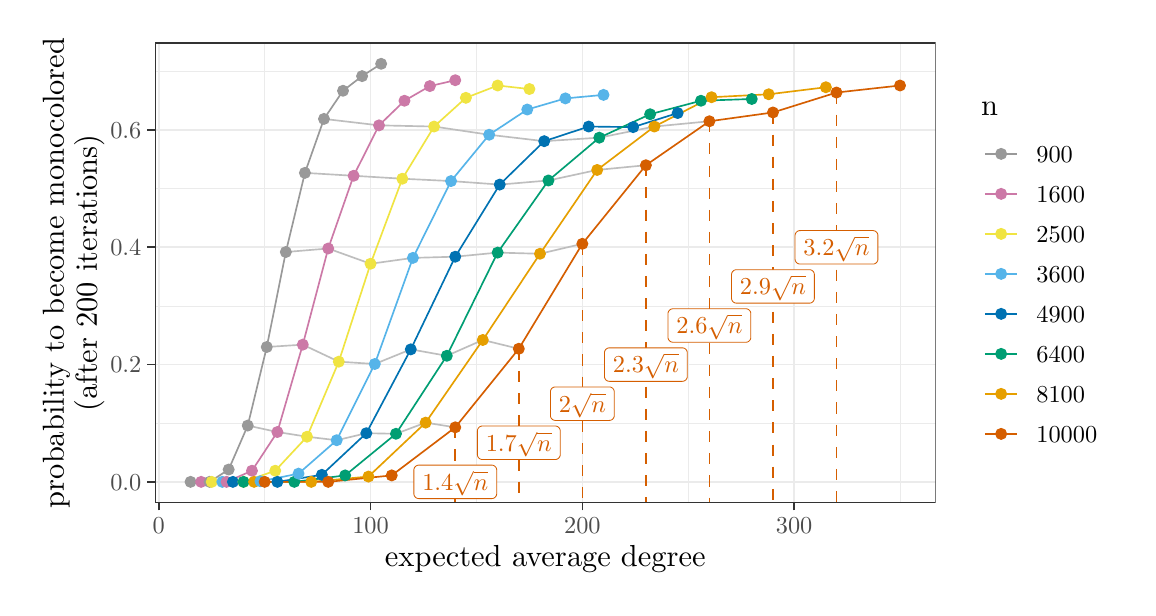
\begin{tikzpicture}[x=1pt,y=1pt]
\definecolor{fillColor}{RGB}{255,255,255}
\path[use as bounding box,fill=fillColor,fill opacity=0.00] (0,0) rectangle (397.48,202.36);
\begin{scope}
\path[clip] (  0.00,  0.00) rectangle (397.48,202.36);
\definecolor{drawColor}{RGB}{255,255,255}
\definecolor{fillColor}{RGB}{255,255,255}

\path[draw=drawColor,line width= 0.6pt,line join=round,line cap=round,fill=fillColor] (  0.00,  0.00) rectangle (397.48,202.36);
\end{scope}
\begin{scope}
\path[clip] ( 46.04, 30.69) rectangle (328.04,196.86);
\definecolor{fillColor}{RGB}{255,255,255}

\path[fill=fillColor] ( 46.04, 30.69) rectangle (328.04,196.86);
\definecolor{drawColor}{gray}{0.92}

\path[draw=drawColor,line width= 0.3pt,line join=round] ( 46.04, 59.43) --
	(328.04, 59.43);

\path[draw=drawColor,line width= 0.3pt,line join=round] ( 46.04,101.80) --
	(328.04,101.80);

\path[draw=drawColor,line width= 0.3pt,line join=round] ( 46.04,144.17) --
	(328.04,144.17);

\path[draw=drawColor,line width= 0.3pt,line join=round] ( 46.04,186.55) --
	(328.04,186.55);

\path[draw=drawColor,line width= 0.3pt,line join=round] ( 85.64, 30.69) --
	( 85.64,196.86);

\path[draw=drawColor,line width= 0.3pt,line join=round] (162.17, 30.69) --
	(162.17,196.86);

\path[draw=drawColor,line width= 0.3pt,line join=round] (238.69, 30.69) --
	(238.69,196.86);

\path[draw=drawColor,line width= 0.3pt,line join=round] (315.22, 30.69) --
	(315.22,196.86);

\path[draw=drawColor,line width= 0.6pt,line join=round] ( 46.04, 38.24) --
	(328.04, 38.24);

\path[draw=drawColor,line width= 0.6pt,line join=round] ( 46.04, 80.61) --
	(328.04, 80.61);

\path[draw=drawColor,line width= 0.6pt,line join=round] ( 46.04,122.99) --
	(328.04,122.99);

\path[draw=drawColor,line width= 0.6pt,line join=round] ( 46.04,165.36) --
	(328.04,165.36);

\path[draw=drawColor,line width= 0.6pt,line join=round] ( 47.38, 30.69) --
	( 47.38,196.86);

\path[draw=drawColor,line width= 0.6pt,line join=round] (123.90, 30.69) --
	(123.90,196.86);

\path[draw=drawColor,line width= 0.6pt,line join=round] (200.43, 30.69) --
	(200.43,196.86);

\path[draw=drawColor,line width= 0.6pt,line join=round] (276.95, 30.69) --
	(276.95,196.86);
\definecolor{drawColor}{RGB}{190,190,190}

\path[draw=drawColor,line width= 0.6pt,line join=round] ( 79.52, 58.58) --
	( 90.23, 56.25) --
	(100.94, 54.55) --
	(111.66, 53.28) --
	(122.37, 55.82) --
	(133.08, 55.61) --
	(143.80, 59.64) --
	(154.51, 57.94);

\path[draw=drawColor,line width= 0.6pt,line join=round] ( 86.40, 86.97) --
	( 99.41, 87.82) --
	(112.42, 81.67) --
	(125.43, 80.83) --
	(138.44, 86.12) --
	(151.45, 83.79) --
	(164.46, 89.51) --
	(177.47, 86.33);

\path[draw=drawColor,line width= 0.6pt,line join=round] ( 93.29,121.29) --
	(108.60,122.56) --
	(123.90,117.05) --
	(139.21,119.17) --
	(154.51,119.60) --
	(169.82,121.08) --
	(185.12,120.66) --
	(200.43,124.26);

\path[draw=drawColor,line width= 0.6pt,line join=round] (100.18,149.89) --
	(117.78,148.84) --
	(135.38,147.78) --
	(152.98,146.93) --
	(170.58,145.66) --
	(188.18,147.14) --
	(205.79,150.95) --
	(223.39,152.65);

\path[draw=drawColor,line width= 0.6pt,line join=round] (107.07,169.39) --
	(126.96,167.06) --
	(146.86,166.63) --
	(166.76,163.67) --
	(186.65,161.34) --
	(206.55,162.61) --
	(226.45,166.63) --
	(246.34,168.54);
\definecolor{drawColor}{gray}{0.60}

\path[draw=drawColor,line width= 0.6pt,line join=round] ( 58.85, 38.24) --
	( 65.74, 38.24) --
	( 72.63, 42.69) --
	( 79.52, 58.58) --
	( 86.40, 86.97) --
	( 93.29,121.29) --
	(100.18,149.89) --
	(107.07,169.39) --
	(113.95,179.56) --
	(120.84,184.85) --
	(127.73,189.30);
\definecolor{drawColor}{RGB}{204,121,167}

\path[draw=drawColor,line width= 0.6pt,line join=round] ( 62.68, 38.24) --
	( 71.86, 38.24) --
	( 81.05, 42.26) --
	( 90.23, 56.25) --
	( 99.41, 87.82) --
	(108.60,122.56) --
	(117.78,148.84) --
	(126.96,167.06) --
	(136.15,175.95) --
	(145.33,181.25) --
	(154.51,183.37);
\definecolor{drawColor}{RGB}{240,228,66}

\path[draw=drawColor,line width= 0.6pt,line join=round] ( 66.51, 38.24) --
	( 77.99, 38.24) --
	( 89.46, 42.26) --
	(100.94, 54.55) --
	(112.42, 81.67) --
	(123.90,117.05) --
	(135.38,147.78) --
	(146.86,166.63) --
	(158.34,177.01) --
	(169.82,181.46) --
	(181.30,180.19);
\definecolor{drawColor}{RGB}{86,180,233}

\path[draw=drawColor,line width= 0.6pt,line join=round] ( 70.33, 38.24) --
	( 84.11, 38.45) --
	( 97.88, 41.21) --
	(111.66, 53.28) --
	(125.43, 80.83) --
	(139.21,119.17) --
	(152.98,146.93) --
	(166.76,163.67) --
	(180.53,172.78) --
	(194.31,176.80) --
	(208.08,178.07);
\definecolor{drawColor}{RGB}{0,114,178}

\path[draw=drawColor,line width= 0.6pt,line join=round] ( 74.16, 38.24) --
	( 90.23, 38.24) --
	(106.30, 40.78) --
	(122.37, 55.82) --
	(138.44, 86.12) --
	(154.51,119.60) --
	(170.58,145.66) --
	(186.65,161.34) --
	(202.72,166.63) --
	(218.79,166.42) --
	(234.87,171.51);
\definecolor{drawColor}{RGB}{0,158,115}

\path[draw=drawColor,line width= 0.6pt,line join=round] ( 77.99, 38.24) --
	( 96.35, 38.24) --
	(114.72, 40.57) --
	(133.08, 55.61) --
	(151.45, 83.79) --
	(169.82,121.08) --
	(188.18,147.14) --
	(206.55,162.61) --
	(224.92,171.08) --
	(243.28,175.95) --
	(261.65,176.59);
\definecolor{drawColor}{RGB}{230,159,0}

\path[draw=drawColor,line width= 0.6pt,line join=round] ( 81.81, 38.24) --
	(102.47, 38.24) --
	(123.14, 40.15) --
	(143.80, 59.64) --
	(164.46, 89.51) --
	(185.12,120.66) --
	(205.79,150.95) --
	(226.45,166.63) --
	(247.11,177.23) --
	(267.77,178.29) --
	(288.43,180.83);
\definecolor{drawColor}{RGB}{213,94,0}

\path[draw=drawColor,line width= 0.6pt,line join=round] ( 85.64, 38.24) --
	(108.60, 38.24) --
	(131.55, 40.57) --
	(154.51, 57.94) --
	(177.47, 86.33) --
	(200.43,124.26) --
	(223.39,152.65) --
	(246.34,168.54) --
	(269.30,171.72) --
	(292.26,178.92) --
	(315.22,181.46);
\definecolor{drawColor}{gray}{0.60}
\definecolor{fillColor}{gray}{0.60}

\path[draw=drawColor,line width= 0.4pt,line join=round,line cap=round,fill=fillColor] ( 58.85, 38.24) circle (  1.96);
\definecolor{drawColor}{RGB}{204,121,167}
\definecolor{fillColor}{RGB}{204,121,167}

\path[draw=drawColor,line width= 0.4pt,line join=round,line cap=round,fill=fillColor] ( 62.68, 38.24) circle (  1.96);
\definecolor{drawColor}{gray}{0.60}
\definecolor{fillColor}{gray}{0.60}

\path[draw=drawColor,line width= 0.4pt,line join=round,line cap=round,fill=fillColor] ( 65.74, 38.24) circle (  1.96);
\definecolor{drawColor}{RGB}{240,228,66}
\definecolor{fillColor}{RGB}{240,228,66}

\path[draw=drawColor,line width= 0.4pt,line join=round,line cap=round,fill=fillColor] ( 66.51, 38.24) circle (  1.96);
\definecolor{drawColor}{RGB}{86,180,233}
\definecolor{fillColor}{RGB}{86,180,233}

\path[draw=drawColor,line width= 0.4pt,line join=round,line cap=round,fill=fillColor] ( 70.33, 38.24) circle (  1.96);
\definecolor{drawColor}{RGB}{204,121,167}
\definecolor{fillColor}{RGB}{204,121,167}

\path[draw=drawColor,line width= 0.4pt,line join=round,line cap=round,fill=fillColor] ( 71.86, 38.24) circle (  1.96);
\definecolor{drawColor}{gray}{0.60}
\definecolor{fillColor}{gray}{0.60}

\path[draw=drawColor,line width= 0.4pt,line join=round,line cap=round,fill=fillColor] ( 72.63, 42.69) circle (  1.96);
\definecolor{drawColor}{RGB}{0,114,178}
\definecolor{fillColor}{RGB}{0,114,178}

\path[draw=drawColor,line width= 0.4pt,line join=round,line cap=round,fill=fillColor] ( 74.16, 38.24) circle (  1.96);
\definecolor{drawColor}{RGB}{240,228,66}
\definecolor{fillColor}{RGB}{240,228,66}

\path[draw=drawColor,line width= 0.4pt,line join=round,line cap=round,fill=fillColor] ( 77.99, 38.24) circle (  1.96);
\definecolor{drawColor}{RGB}{0,158,115}
\definecolor{fillColor}{RGB}{0,158,115}

\path[draw=drawColor,line width= 0.4pt,line join=round,line cap=round,fill=fillColor] ( 77.99, 38.24) circle (  1.96);
\definecolor{drawColor}{gray}{0.60}
\definecolor{fillColor}{gray}{0.60}

\path[draw=drawColor,line width= 0.4pt,line join=round,line cap=round,fill=fillColor] ( 79.52, 58.58) circle (  1.96);
\definecolor{drawColor}{RGB}{204,121,167}
\definecolor{fillColor}{RGB}{204,121,167}

\path[draw=drawColor,line width= 0.4pt,line join=round,line cap=round,fill=fillColor] ( 81.05, 42.26) circle (  1.96);
\definecolor{drawColor}{RGB}{230,159,0}
\definecolor{fillColor}{RGB}{230,159,0}

\path[draw=drawColor,line width= 0.4pt,line join=round,line cap=round,fill=fillColor] ( 81.81, 38.24) circle (  1.96);
\definecolor{drawColor}{RGB}{86,180,233}
\definecolor{fillColor}{RGB}{86,180,233}

\path[draw=drawColor,line width= 0.4pt,line join=round,line cap=round,fill=fillColor] ( 84.11, 38.45) circle (  1.96);
\definecolor{drawColor}{RGB}{213,94,0}
\definecolor{fillColor}{RGB}{213,94,0}

\path[draw=drawColor,line width= 0.4pt,line join=round,line cap=round,fill=fillColor] ( 85.64, 38.24) circle (  1.96);
\definecolor{drawColor}{gray}{0.60}
\definecolor{fillColor}{gray}{0.60}

\path[draw=drawColor,line width= 0.4pt,line join=round,line cap=round,fill=fillColor] ( 86.40, 86.97) circle (  1.96);
\definecolor{drawColor}{RGB}{240,228,66}
\definecolor{fillColor}{RGB}{240,228,66}

\path[draw=drawColor,line width= 0.4pt,line join=round,line cap=round,fill=fillColor] ( 89.46, 42.26) circle (  1.96);
\definecolor{drawColor}{RGB}{204,121,167}
\definecolor{fillColor}{RGB}{204,121,167}

\path[draw=drawColor,line width= 0.4pt,line join=round,line cap=round,fill=fillColor] ( 90.23, 56.25) circle (  1.96);
\definecolor{drawColor}{RGB}{0,114,178}
\definecolor{fillColor}{RGB}{0,114,178}

\path[draw=drawColor,line width= 0.4pt,line join=round,line cap=round,fill=fillColor] ( 90.23, 38.24) circle (  1.96);
\definecolor{drawColor}{gray}{0.60}
\definecolor{fillColor}{gray}{0.60}

\path[draw=drawColor,line width= 0.4pt,line join=round,line cap=round,fill=fillColor] ( 93.29,121.29) circle (  1.96);
\definecolor{drawColor}{RGB}{0,158,115}
\definecolor{fillColor}{RGB}{0,158,115}

\path[draw=drawColor,line width= 0.4pt,line join=round,line cap=round,fill=fillColor] ( 96.35, 38.24) circle (  1.96);
\definecolor{drawColor}{RGB}{86,180,233}
\definecolor{fillColor}{RGB}{86,180,233}

\path[draw=drawColor,line width= 0.4pt,line join=round,line cap=round,fill=fillColor] ( 97.88, 41.21) circle (  1.96);
\definecolor{drawColor}{RGB}{204,121,167}
\definecolor{fillColor}{RGB}{204,121,167}

\path[draw=drawColor,line width= 0.4pt,line join=round,line cap=round,fill=fillColor] ( 99.41, 87.82) circle (  1.96);
\definecolor{drawColor}{gray}{0.60}
\definecolor{fillColor}{gray}{0.60}

\path[draw=drawColor,line width= 0.4pt,line join=round,line cap=round,fill=fillColor] (100.18,149.89) circle (  1.96);
\definecolor{drawColor}{RGB}{240,228,66}
\definecolor{fillColor}{RGB}{240,228,66}

\path[draw=drawColor,line width= 0.4pt,line join=round,line cap=round,fill=fillColor] (100.94, 54.55) circle (  1.96);
\definecolor{drawColor}{RGB}{230,159,0}
\definecolor{fillColor}{RGB}{230,159,0}

\path[draw=drawColor,line width= 0.4pt,line join=round,line cap=round,fill=fillColor] (102.47, 38.24) circle (  1.96);
\definecolor{drawColor}{RGB}{0,114,178}
\definecolor{fillColor}{RGB}{0,114,178}

\path[draw=drawColor,line width= 0.4pt,line join=round,line cap=round,fill=fillColor] (106.30, 40.78) circle (  1.96);
\definecolor{drawColor}{gray}{0.60}
\definecolor{fillColor}{gray}{0.60}

\path[draw=drawColor,line width= 0.4pt,line join=round,line cap=round,fill=fillColor] (107.07,169.39) circle (  1.96);
\definecolor{drawColor}{RGB}{204,121,167}
\definecolor{fillColor}{RGB}{204,121,167}

\path[draw=drawColor,line width= 0.4pt,line join=round,line cap=round,fill=fillColor] (108.60,122.56) circle (  1.96);
\definecolor{drawColor}{RGB}{213,94,0}
\definecolor{fillColor}{RGB}{213,94,0}

\path[draw=drawColor,line width= 0.4pt,line join=round,line cap=round,fill=fillColor] (108.60, 38.24) circle (  1.96);
\definecolor{drawColor}{RGB}{86,180,233}
\definecolor{fillColor}{RGB}{86,180,233}

\path[draw=drawColor,line width= 0.4pt,line join=round,line cap=round,fill=fillColor] (111.66, 53.28) circle (  1.96);
\definecolor{drawColor}{RGB}{240,228,66}
\definecolor{fillColor}{RGB}{240,228,66}

\path[draw=drawColor,line width= 0.4pt,line join=round,line cap=round,fill=fillColor] (112.42, 81.67) circle (  1.96);
\definecolor{drawColor}{gray}{0.60}
\definecolor{fillColor}{gray}{0.60}

\path[draw=drawColor,line width= 0.4pt,line join=round,line cap=round,fill=fillColor] (113.95,179.56) circle (  1.96);
\definecolor{drawColor}{RGB}{0,158,115}
\definecolor{fillColor}{RGB}{0,158,115}

\path[draw=drawColor,line width= 0.4pt,line join=round,line cap=round,fill=fillColor] (114.72, 40.57) circle (  1.96);
\definecolor{drawColor}{RGB}{204,121,167}
\definecolor{fillColor}{RGB}{204,121,167}

\path[draw=drawColor,line width= 0.4pt,line join=round,line cap=round,fill=fillColor] (117.78,148.84) circle (  1.96);
\definecolor{drawColor}{gray}{0.60}
\definecolor{fillColor}{gray}{0.60}

\path[draw=drawColor,line width= 0.4pt,line join=round,line cap=round,fill=fillColor] (120.84,184.85) circle (  1.96);
\definecolor{drawColor}{RGB}{0,114,178}
\definecolor{fillColor}{RGB}{0,114,178}

\path[draw=drawColor,line width= 0.4pt,line join=round,line cap=round,fill=fillColor] (122.37, 55.82) circle (  1.96);
\definecolor{drawColor}{RGB}{230,159,0}
\definecolor{fillColor}{RGB}{230,159,0}

\path[draw=drawColor,line width= 0.4pt,line join=round,line cap=round,fill=fillColor] (123.14, 40.15) circle (  1.96);
\definecolor{drawColor}{RGB}{240,228,66}
\definecolor{fillColor}{RGB}{240,228,66}

\path[draw=drawColor,line width= 0.4pt,line join=round,line cap=round,fill=fillColor] (123.90,117.05) circle (  1.96);
\definecolor{drawColor}{RGB}{86,180,233}
\definecolor{fillColor}{RGB}{86,180,233}

\path[draw=drawColor,line width= 0.4pt,line join=round,line cap=round,fill=fillColor] (125.43, 80.83) circle (  1.96);
\definecolor{drawColor}{RGB}{204,121,167}
\definecolor{fillColor}{RGB}{204,121,167}

\path[draw=drawColor,line width= 0.4pt,line join=round,line cap=round,fill=fillColor] (126.96,167.06) circle (  1.96);
\definecolor{drawColor}{gray}{0.60}
\definecolor{fillColor}{gray}{0.60}

\path[draw=drawColor,line width= 0.4pt,line join=round,line cap=round,fill=fillColor] (127.73,189.30) circle (  1.96);
\definecolor{drawColor}{RGB}{213,94,0}
\definecolor{fillColor}{RGB}{213,94,0}

\path[draw=drawColor,line width= 0.4pt,line join=round,line cap=round,fill=fillColor] (131.55, 40.57) circle (  1.96);
\definecolor{drawColor}{RGB}{0,158,115}
\definecolor{fillColor}{RGB}{0,158,115}

\path[draw=drawColor,line width= 0.4pt,line join=round,line cap=round,fill=fillColor] (133.08, 55.61) circle (  1.96);
\definecolor{drawColor}{RGB}{240,228,66}
\definecolor{fillColor}{RGB}{240,228,66}

\path[draw=drawColor,line width= 0.4pt,line join=round,line cap=round,fill=fillColor] (135.38,147.78) circle (  1.96);
\definecolor{drawColor}{RGB}{204,121,167}
\definecolor{fillColor}{RGB}{204,121,167}

\path[draw=drawColor,line width= 0.4pt,line join=round,line cap=round,fill=fillColor] (136.15,175.95) circle (  1.96);
\definecolor{drawColor}{RGB}{0,114,178}
\definecolor{fillColor}{RGB}{0,114,178}

\path[draw=drawColor,line width= 0.4pt,line join=round,line cap=round,fill=fillColor] (138.44, 86.12) circle (  1.96);
\definecolor{drawColor}{RGB}{86,180,233}
\definecolor{fillColor}{RGB}{86,180,233}

\path[draw=drawColor,line width= 0.4pt,line join=round,line cap=round,fill=fillColor] (139.21,119.17) circle (  1.96);
\definecolor{drawColor}{RGB}{230,159,0}
\definecolor{fillColor}{RGB}{230,159,0}

\path[draw=drawColor,line width= 0.4pt,line join=round,line cap=round,fill=fillColor] (143.80, 59.64) circle (  1.96);
\definecolor{drawColor}{RGB}{204,121,167}
\definecolor{fillColor}{RGB}{204,121,167}

\path[draw=drawColor,line width= 0.4pt,line join=round,line cap=round,fill=fillColor] (145.33,181.25) circle (  1.96);
\definecolor{drawColor}{RGB}{240,228,66}
\definecolor{fillColor}{RGB}{240,228,66}

\path[draw=drawColor,line width= 0.4pt,line join=round,line cap=round,fill=fillColor] (146.86,166.63) circle (  1.96);
\definecolor{drawColor}{RGB}{0,158,115}
\definecolor{fillColor}{RGB}{0,158,115}

\path[draw=drawColor,line width= 0.4pt,line join=round,line cap=round,fill=fillColor] (151.45, 83.79) circle (  1.96);
\definecolor{drawColor}{RGB}{86,180,233}
\definecolor{fillColor}{RGB}{86,180,233}

\path[draw=drawColor,line width= 0.4pt,line join=round,line cap=round,fill=fillColor] (152.98,146.93) circle (  1.96);
\definecolor{drawColor}{RGB}{204,121,167}
\definecolor{fillColor}{RGB}{204,121,167}

\path[draw=drawColor,line width= 0.4pt,line join=round,line cap=round,fill=fillColor] (154.51,183.37) circle (  1.96);
\definecolor{drawColor}{RGB}{0,114,178}
\definecolor{fillColor}{RGB}{0,114,178}

\path[draw=drawColor,line width= 0.4pt,line join=round,line cap=round,fill=fillColor] (154.51,119.60) circle (  1.96);
\definecolor{drawColor}{RGB}{213,94,0}
\definecolor{fillColor}{RGB}{213,94,0}

\path[draw=drawColor,line width= 0.4pt,line join=round,line cap=round,fill=fillColor] (154.51, 57.94) circle (  1.96);
\definecolor{drawColor}{RGB}{240,228,66}
\definecolor{fillColor}{RGB}{240,228,66}

\path[draw=drawColor,line width= 0.4pt,line join=round,line cap=round,fill=fillColor] (158.34,177.01) circle (  1.96);
\definecolor{drawColor}{RGB}{230,159,0}
\definecolor{fillColor}{RGB}{230,159,0}

\path[draw=drawColor,line width= 0.4pt,line join=round,line cap=round,fill=fillColor] (164.46, 89.51) circle (  1.96);
\definecolor{drawColor}{RGB}{86,180,233}
\definecolor{fillColor}{RGB}{86,180,233}

\path[draw=drawColor,line width= 0.4pt,line join=round,line cap=round,fill=fillColor] (166.76,163.67) circle (  1.96);
\definecolor{drawColor}{RGB}{240,228,66}
\definecolor{fillColor}{RGB}{240,228,66}

\path[draw=drawColor,line width= 0.4pt,line join=round,line cap=round,fill=fillColor] (169.82,181.46) circle (  1.96);
\definecolor{drawColor}{RGB}{0,158,115}
\definecolor{fillColor}{RGB}{0,158,115}

\path[draw=drawColor,line width= 0.4pt,line join=round,line cap=round,fill=fillColor] (169.82,121.08) circle (  1.96);
\definecolor{drawColor}{RGB}{0,114,178}
\definecolor{fillColor}{RGB}{0,114,178}

\path[draw=drawColor,line width= 0.4pt,line join=round,line cap=round,fill=fillColor] (170.58,145.66) circle (  1.96);
\definecolor{drawColor}{RGB}{213,94,0}
\definecolor{fillColor}{RGB}{213,94,0}

\path[draw=drawColor,line width= 0.4pt,line join=round,line cap=round,fill=fillColor] (177.47, 86.33) circle (  1.96);
\definecolor{drawColor}{RGB}{86,180,233}
\definecolor{fillColor}{RGB}{86,180,233}

\path[draw=drawColor,line width= 0.4pt,line join=round,line cap=round,fill=fillColor] (180.53,172.78) circle (  1.96);
\definecolor{drawColor}{RGB}{240,228,66}
\definecolor{fillColor}{RGB}{240,228,66}

\path[draw=drawColor,line width= 0.4pt,line join=round,line cap=round,fill=fillColor] (181.30,180.19) circle (  1.96);
\definecolor{drawColor}{RGB}{230,159,0}
\definecolor{fillColor}{RGB}{230,159,0}

\path[draw=drawColor,line width= 0.4pt,line join=round,line cap=round,fill=fillColor] (185.12,120.66) circle (  1.96);
\definecolor{drawColor}{RGB}{0,114,178}
\definecolor{fillColor}{RGB}{0,114,178}

\path[draw=drawColor,line width= 0.4pt,line join=round,line cap=round,fill=fillColor] (186.65,161.34) circle (  1.96);
\definecolor{drawColor}{RGB}{0,158,115}
\definecolor{fillColor}{RGB}{0,158,115}

\path[draw=drawColor,line width= 0.4pt,line join=round,line cap=round,fill=fillColor] (188.18,147.14) circle (  1.96);
\definecolor{drawColor}{RGB}{86,180,233}
\definecolor{fillColor}{RGB}{86,180,233}

\path[draw=drawColor,line width= 0.4pt,line join=round,line cap=round,fill=fillColor] (194.31,176.80) circle (  1.96);
\definecolor{drawColor}{RGB}{213,94,0}
\definecolor{fillColor}{RGB}{213,94,0}

\path[draw=drawColor,line width= 0.4pt,line join=round,line cap=round,fill=fillColor] (200.43,124.26) circle (  1.96);
\definecolor{drawColor}{RGB}{0,114,178}
\definecolor{fillColor}{RGB}{0,114,178}

\path[draw=drawColor,line width= 0.4pt,line join=round,line cap=round,fill=fillColor] (202.72,166.63) circle (  1.96);
\definecolor{drawColor}{RGB}{230,159,0}
\definecolor{fillColor}{RGB}{230,159,0}

\path[draw=drawColor,line width= 0.4pt,line join=round,line cap=round,fill=fillColor] (205.79,150.95) circle (  1.96);
\definecolor{drawColor}{RGB}{0,158,115}
\definecolor{fillColor}{RGB}{0,158,115}

\path[draw=drawColor,line width= 0.4pt,line join=round,line cap=round,fill=fillColor] (206.55,162.61) circle (  1.96);
\definecolor{drawColor}{RGB}{86,180,233}
\definecolor{fillColor}{RGB}{86,180,233}

\path[draw=drawColor,line width= 0.4pt,line join=round,line cap=round,fill=fillColor] (208.08,178.07) circle (  1.96);
\definecolor{drawColor}{RGB}{0,114,178}
\definecolor{fillColor}{RGB}{0,114,178}

\path[draw=drawColor,line width= 0.4pt,line join=round,line cap=round,fill=fillColor] (218.79,166.42) circle (  1.96);
\definecolor{drawColor}{RGB}{213,94,0}
\definecolor{fillColor}{RGB}{213,94,0}

\path[draw=drawColor,line width= 0.4pt,line join=round,line cap=round,fill=fillColor] (223.39,152.65) circle (  1.96);
\definecolor{drawColor}{RGB}{0,158,115}
\definecolor{fillColor}{RGB}{0,158,115}

\path[draw=drawColor,line width= 0.4pt,line join=round,line cap=round,fill=fillColor] (224.92,171.08) circle (  1.96);
\definecolor{drawColor}{RGB}{230,159,0}
\definecolor{fillColor}{RGB}{230,159,0}

\path[draw=drawColor,line width= 0.4pt,line join=round,line cap=round,fill=fillColor] (226.45,166.63) circle (  1.96);
\definecolor{drawColor}{RGB}{0,114,178}
\definecolor{fillColor}{RGB}{0,114,178}

\path[draw=drawColor,line width= 0.4pt,line join=round,line cap=round,fill=fillColor] (234.87,171.51) circle (  1.96);
\definecolor{drawColor}{RGB}{0,158,115}
\definecolor{fillColor}{RGB}{0,158,115}

\path[draw=drawColor,line width= 0.4pt,line join=round,line cap=round,fill=fillColor] (243.28,175.95) circle (  1.96);
\definecolor{drawColor}{RGB}{213,94,0}
\definecolor{fillColor}{RGB}{213,94,0}

\path[draw=drawColor,line width= 0.4pt,line join=round,line cap=round,fill=fillColor] (246.34,168.54) circle (  1.96);
\definecolor{drawColor}{RGB}{230,159,0}
\definecolor{fillColor}{RGB}{230,159,0}

\path[draw=drawColor,line width= 0.4pt,line join=round,line cap=round,fill=fillColor] (247.11,177.23) circle (  1.96);
\definecolor{drawColor}{RGB}{0,158,115}
\definecolor{fillColor}{RGB}{0,158,115}

\path[draw=drawColor,line width= 0.4pt,line join=round,line cap=round,fill=fillColor] (261.65,176.59) circle (  1.96);
\definecolor{drawColor}{RGB}{230,159,0}
\definecolor{fillColor}{RGB}{230,159,0}

\path[draw=drawColor,line width= 0.4pt,line join=round,line cap=round,fill=fillColor] (267.77,178.29) circle (  1.96);
\definecolor{drawColor}{RGB}{213,94,0}
\definecolor{fillColor}{RGB}{213,94,0}

\path[draw=drawColor,line width= 0.4pt,line join=round,line cap=round,fill=fillColor] (269.30,171.72) circle (  1.96);
\definecolor{drawColor}{RGB}{230,159,0}
\definecolor{fillColor}{RGB}{230,159,0}

\path[draw=drawColor,line width= 0.4pt,line join=round,line cap=round,fill=fillColor] (288.43,180.83) circle (  1.96);
\definecolor{drawColor}{RGB}{213,94,0}
\definecolor{fillColor}{RGB}{213,94,0}

\path[draw=drawColor,line width= 0.4pt,line join=round,line cap=round,fill=fillColor] (292.26,178.92) circle (  1.96);

\path[draw=drawColor,line width= 0.4pt,line join=round,line cap=round,fill=fillColor] (315.22,181.46) circle (  1.96);

\path[draw=drawColor,line width= 0.6pt,dash pattern=on 4pt off 4pt ,line join=round] (154.51, 57.94) -- (154.51, 30.69);

\path[draw=drawColor,line width= 0.6pt,dash pattern=on 4pt off 4pt ,line join=round] (177.47, 86.33) -- (177.47, 30.69);

\path[draw=drawColor,line width= 0.6pt,dash pattern=on 4pt off 4pt ,line join=round] (200.43,124.26) -- (200.43, 30.69);

\path[draw=drawColor,line width= 0.6pt,dash pattern=on 4pt off 4pt ,line join=round] (223.39,152.65) -- (223.39, 30.69);

\path[draw=drawColor,line width= 0.6pt,dash pattern=on 4pt off 4pt ,line join=round] (246.34,168.54) -- (246.34, 30.69);

\path[draw=drawColor,line width= 0.6pt,dash pattern=on 4pt off 4pt ,line join=round] (269.30,171.72) -- (269.30, 30.69);

\path[draw=drawColor,line width= 0.6pt,dash pattern=on 4pt off 4pt ,line join=round] (292.26,178.92) -- (292.26, 30.69);
\definecolor{fillColor}{RGB}{255,255,255}

\path[draw=drawColor,line width= 0.3pt,line join=round,line cap=round,fill=fillColor] (141.35, 32.19) --
	(167.67, 32.19) --
	(167.60, 32.19) --
	(167.89, 32.20) --
	(168.18, 32.26) --
	(168.45, 32.36) --
	(168.70, 32.51) --
	(168.93, 32.69) --
	(169.12, 32.91) --
	(169.27, 33.16) --
	(169.39, 33.43) --
	(169.46, 33.71) --
	(169.48, 34.00) --
	(169.48, 34.00) --
	(169.48, 42.48) --
	(169.48, 42.48) --
	(169.46, 42.77) --
	(169.39, 43.05) --
	(169.27, 43.32) --
	(169.12, 43.57) --
	(168.93, 43.78) --
	(168.70, 43.97) --
	(168.45, 44.11) --
	(168.18, 44.22) --
	(167.89, 44.27) --
	(167.67, 44.29) --
	(141.35, 44.29) --
	(141.57, 44.27) --
	(141.28, 44.29) --
	(140.99, 44.25) --
	(140.71, 44.17) --
	(140.45, 44.05) --
	(140.21, 43.88) --
	(140.00, 43.68) --
	(139.82, 43.45) --
	(139.69, 43.19) --
	(139.60, 42.91) --
	(139.55, 42.63) --
	(139.54, 42.48) --
	(139.54, 34.00) --
	(139.55, 34.14) --
	(139.55, 33.85) --
	(139.60, 33.56) --
	(139.69, 33.29) --
	(139.82, 33.03) --
	(140.00, 32.80) --
	(140.21, 32.60) --
	(140.45, 32.43) --
	(140.71, 32.31) --
	(140.99, 32.23) --
	(141.28, 32.19) --
	cycle;
\end{scope}
\begin{scope}
\path[clip] ( 46.04, 30.69) rectangle (328.04,196.86);
\definecolor{drawColor}{RGB}{213,94,0}

\node[text=drawColor,anchor=base,inner sep=0pt, outer sep=0pt, scale=  0.88] at (154.51, 35.20) {$1.4\sqrt{n}$};
\definecolor{fillColor}{RGB}{255,255,255}

\path[draw=drawColor,line width= 0.3pt,line join=round,line cap=round,fill=fillColor] (164.31, 46.32) --
	(190.63, 46.32) --
	(190.56, 46.32) --
	(190.85, 46.33) --
	(191.13, 46.39) --
	(191.41, 46.49) --
	(191.66, 46.64) --
	(191.88, 46.82) --
	(192.08, 47.04) --
	(192.23, 47.28) --
	(192.35, 47.55) --
	(192.42, 47.83) --
	(192.44, 48.12) --
	(192.44, 48.12) --
	(192.44, 56.61) --
	(192.44, 56.61) --
	(192.42, 56.90) --
	(192.35, 57.18) --
	(192.23, 57.45) --
	(192.08, 57.69) --
	(191.88, 57.91) --
	(191.66, 58.09) --
	(191.41, 58.24) --
	(191.13, 58.34) --
	(190.85, 58.40) --
	(190.63, 58.41) --
	(164.31, 58.41) --
	(164.53, 58.40) --
	(164.24, 58.41) --
	(163.95, 58.38) --
	(163.67, 58.29) --
	(163.41, 58.17) --
	(163.17, 58.01) --
	(162.96, 57.80) --
	(162.78, 57.57) --
	(162.65, 57.31) --
	(162.55, 57.04) --
	(162.51, 56.75) --
	(162.50, 56.61) --
	(162.50, 48.12) --
	(162.51, 48.27) --
	(162.51, 47.98) --
	(162.55, 47.69) --
	(162.65, 47.41) --
	(162.78, 47.16) --
	(162.96, 46.92) --
	(163.17, 46.72) --
	(163.41, 46.56) --
	(163.67, 46.43) --
	(163.95, 46.35) --
	(164.24, 46.32) --
	cycle;
\end{scope}
\begin{scope}
\path[clip] ( 46.04, 30.69) rectangle (328.04,196.86);
\definecolor{drawColor}{RGB}{213,94,0}

\node[text=drawColor,anchor=base,inner sep=0pt, outer sep=0pt, scale=  0.88] at (177.47, 49.33) {$1.7\sqrt{n}$};
\definecolor{fillColor}{RGB}{255,255,255}

\path[draw=drawColor,line width= 0.3pt,line join=round,line cap=round,fill=fillColor] (190.70, 60.44) --
	(210.16, 60.44) --
	(210.09, 60.44) --
	(210.38, 60.45) --
	(210.66, 60.51) --
	(210.93, 60.61) --
	(211.19, 60.76) --
	(211.41, 60.94) --
	(211.60, 61.16) --
	(211.76, 61.41) --
	(211.87, 61.67) --
	(211.94, 61.96) --
	(211.97, 62.25) --
	(211.97, 62.25) --
	(211.97, 70.73) --
	(211.97, 70.73) --
	(211.94, 71.02) --
	(211.87, 71.30) --
	(211.76, 71.57) --
	(211.60, 71.82) --
	(211.41, 72.03) --
	(211.19, 72.22) --
	(210.93, 72.36) --
	(210.66, 72.47) --
	(210.38, 72.52) --
	(210.16, 72.54) --
	(190.70, 72.54) --
	(190.91, 72.52) --
	(190.62, 72.54) --
	(190.34, 72.50) --
	(190.06, 72.42) --
	(189.79, 72.29) --
	(189.55, 72.13) --
	(189.34, 71.93) --
	(189.17, 71.70) --
	(189.03, 71.44) --
	(188.94, 71.16) --
	(188.90, 70.88) --
	(188.89, 70.73) --
	(188.89, 62.25) --
	(188.90, 62.39) --
	(188.90, 62.10) --
	(188.94, 61.81) --
	(189.03, 61.54) --
	(189.17, 61.28) --
	(189.34, 61.05) --
	(189.55, 60.85) --
	(189.79, 60.68) --
	(190.06, 60.56) --
	(190.34, 60.48) --
	(190.62, 60.44) --
	cycle;
\end{scope}
\begin{scope}
\path[clip] ( 46.04, 30.69) rectangle (328.04,196.86);
\definecolor{drawColor}{RGB}{213,94,0}

\node[text=drawColor,anchor=base,inner sep=0pt, outer sep=0pt, scale=  0.88] at (200.43, 63.45) {$2\sqrt{n}$};
\definecolor{fillColor}{RGB}{255,255,255}

\path[draw=drawColor,line width= 0.3pt,line join=round,line cap=round,fill=fillColor] (210.22, 74.56) --
	(236.55, 74.56) --
	(236.48, 74.57) --
	(236.77, 74.58) --
	(237.05, 74.64) --
	(237.32, 74.74) --
	(237.57, 74.88) --
	(237.80, 75.07) --
	(237.99, 75.29) --
	(238.15, 75.53) --
	(238.26, 75.80) --
	(238.33, 76.08) --
	(238.35, 76.37) --
	(238.35, 76.37) --
	(238.35, 84.85) --
	(238.35, 84.85) --
	(238.33, 85.14) --
	(238.26, 85.43) --
	(238.15, 85.69) --
	(237.99, 85.94) --
	(237.80, 86.16) --
	(237.57, 86.34) --
	(237.32, 86.49) --
	(237.05, 86.59) --
	(236.77, 86.65) --
	(236.55, 86.66) --
	(210.22, 86.66) --
	(210.44, 86.65) --
	(210.15, 86.66) --
	(209.86, 86.63) --
	(209.58, 86.54) --
	(209.32, 86.42) --
	(209.08, 86.25) --
	(208.87, 86.05) --
	(208.70, 85.82) --
	(208.56, 85.56) --
	(208.47, 85.29) --
	(208.42, 85.00) --
	(208.42, 84.85) --
	(208.42, 76.37) --
	(208.42, 76.52) --
	(208.42, 76.23) --
	(208.47, 75.94) --
	(208.56, 75.66) --
	(208.70, 75.41) --
	(208.87, 75.17) --
	(209.08, 74.97) --
	(209.32, 74.81) --
	(209.58, 74.68) --
	(209.86, 74.60) --
	(210.15, 74.57) --
	cycle;
\end{scope}
\begin{scope}
\path[clip] ( 46.04, 30.69) rectangle (328.04,196.86);
\definecolor{drawColor}{RGB}{213,94,0}

\node[text=drawColor,anchor=base,inner sep=0pt, outer sep=0pt, scale=  0.88] at (223.39, 77.58) {$2.3\sqrt{n}$};
\definecolor{fillColor}{RGB}{255,255,255}

\path[draw=drawColor,line width= 0.3pt,line join=round,line cap=round,fill=fillColor] (233.18, 88.69) --
	(259.51, 88.69) --
	(259.43, 88.69) --
	(259.72, 88.70) --
	(260.01, 88.76) --
	(260.28, 88.86) --
	(260.53, 89.01) --
	(260.76, 89.19) --
	(260.95, 89.41) --
	(261.11, 89.66) --
	(261.22, 89.92) --
	(261.29, 90.21) --
	(261.31, 90.50) --
	(261.31, 90.50) --
	(261.31, 98.98) --
	(261.31, 98.98) --
	(261.29, 99.27) --
	(261.22, 99.55) --
	(261.11, 99.82) --
	(260.95,100.07) --
	(260.76,100.28) --
	(260.53,100.47) --
	(260.28,100.61) --
	(260.01,100.72) --
	(259.72,100.77) --
	(259.51,100.79) --
	(233.18,100.79) --
	(233.40,100.77) --
	(233.11,100.78) --
	(232.82,100.75) --
	(232.54,100.67) --
	(232.28,100.54) --
	(232.04,100.38) --
	(231.83,100.18) --
	(231.66, 99.95) --
	(231.52, 99.69) --
	(231.43, 99.41) --
	(231.38, 99.13) --
	(231.38, 98.98) --
	(231.38, 90.50) --
	(231.38, 90.64) --
	(231.38, 90.35) --
	(231.43, 90.06) --
	(231.52, 89.79) --
	(231.66, 89.53) --
	(231.83, 89.30) --
	(232.04, 89.10) --
	(232.28, 88.93) --
	(232.54, 88.81) --
	(232.82, 88.73) --
	(233.11, 88.69) --
	cycle;
\end{scope}
\begin{scope}
\path[clip] ( 46.04, 30.69) rectangle (328.04,196.86);
\definecolor{drawColor}{RGB}{213,94,0}

\node[text=drawColor,anchor=base,inner sep=0pt, outer sep=0pt, scale=  0.88] at (246.34, 91.70) {$2.6\sqrt{n}$};
\definecolor{fillColor}{RGB}{255,255,255}

\path[draw=drawColor,line width= 0.3pt,line join=round,line cap=round,fill=fillColor] (256.14,102.81) --
	(282.46,102.81) --
	(282.39,102.82) --
	(282.68,102.83) --
	(282.97,102.89) --
	(283.24,102.99) --
	(283.49,103.13) --
	(283.72,103.32) --
	(283.91,103.54) --
	(284.06,103.78) --
	(284.18,104.05) --
	(284.25,104.33) --
	(284.27,104.62) --
	(284.27,104.62) --
	(284.27,113.10) --
	(284.27,113.10) --
	(284.25,113.39) --
	(284.18,113.68) --
	(284.06,113.94) --
	(283.91,114.19) --
	(283.72,114.41) --
	(283.49,114.59) --
	(283.24,114.74) --
	(282.97,114.84) --
	(282.68,114.90) --
	(282.46,114.91) --
	(256.14,114.91) --
	(256.36,114.90) --
	(256.07,114.91) --
	(255.78,114.87) --
	(255.50,114.79) --
	(255.24,114.67) --
	(255.00,114.50) --
	(254.79,114.30) --
	(254.61,114.07) --
	(254.48,113.81) --
	(254.39,113.54) --
	(254.34,113.25) --
	(254.33,113.10) --
	(254.33,104.62) --
	(254.34,104.77) --
	(254.34,104.48) --
	(254.39,104.19) --
	(254.48,103.91) --
	(254.61,103.66) --
	(254.79,103.42) --
	(255.00,103.22) --
	(255.24,103.06) --
	(255.50,102.93) --
	(255.78,102.85) --
	(256.07,102.82) --
	cycle;
\end{scope}
\begin{scope}
\path[clip] ( 46.04, 30.69) rectangle (328.04,196.86);
\definecolor{drawColor}{RGB}{213,94,0}

\node[text=drawColor,anchor=base,inner sep=0pt, outer sep=0pt, scale=  0.88] at (269.30,105.83) {$2.9\sqrt{n}$};
\definecolor{fillColor}{RGB}{255,255,255}

\path[draw=drawColor,line width= 0.3pt,line join=round,line cap=round,fill=fillColor] (279.10,116.94) --
	(305.42,116.94) --
	(305.35,116.94) --
	(305.64,116.95) --
	(305.92,117.01) --
	(306.20,117.11) --
	(306.45,117.26) --
	(306.67,117.44) --
	(306.87,117.66) --
	(307.02,117.91) --
	(307.14,118.17) --
	(307.21,118.46) --
	(307.23,118.75) --
	(307.23,118.75) --
	(307.23,127.23) --
	(307.23,127.23) --
	(307.21,127.52) --
	(307.14,127.80) --
	(307.02,128.07) --
	(306.87,128.31) --
	(306.67,128.53) --
	(306.45,128.72) --
	(306.20,128.86) --
	(305.92,128.96) --
	(305.64,129.02) --
	(305.42,129.04) --
	(279.10,129.04) --
	(279.32,129.02) --
	(279.03,129.03) --
	(278.74,129.00) --
	(278.46,128.92) --
	(278.20,128.79) --
	(277.96,128.63) --
	(277.75,128.43) --
	(277.57,128.19) --
	(277.44,127.94) --
	(277.34,127.66) --
	(277.30,127.37) --
	(277.29,127.23) --
	(277.29,118.75) --
	(277.30,118.89) --
	(277.30,118.60) --
	(277.34,118.31) --
	(277.44,118.04) --
	(277.57,117.78) --
	(277.75,117.55) --
	(277.96,117.35) --
	(278.20,117.18) --
	(278.46,117.06) --
	(278.74,116.98) --
	(279.03,116.94) --
	cycle;
\end{scope}
\begin{scope}
\path[clip] ( 46.04, 30.69) rectangle (328.04,196.86);
\definecolor{drawColor}{RGB}{213,94,0}

\node[text=drawColor,anchor=base,inner sep=0pt, outer sep=0pt, scale=  0.88] at (292.26,119.95) {$3.2\sqrt{n}$};
\definecolor{drawColor}{gray}{0.20}

\path[draw=drawColor,line width= 0.6pt,line join=round,line cap=round] ( 46.04, 30.69) rectangle (328.04,196.86);
\end{scope}
\begin{scope}
\path[clip] (  0.00,  0.00) rectangle (397.48,202.36);
\definecolor{drawColor}{gray}{0.30}

\node[text=drawColor,anchor=base east,inner sep=0pt, outer sep=0pt, scale=  0.88] at ( 41.09, 35.21) {0.0};

\node[text=drawColor,anchor=base east,inner sep=0pt, outer sep=0pt, scale=  0.88] at ( 41.09, 77.58) {0.2};

\node[text=drawColor,anchor=base east,inner sep=0pt, outer sep=0pt, scale=  0.88] at ( 41.09,119.96) {0.4};

\node[text=drawColor,anchor=base east,inner sep=0pt, outer sep=0pt, scale=  0.88] at ( 41.09,162.33) {0.6};
\end{scope}
\begin{scope}
\path[clip] (  0.00,  0.00) rectangle (397.48,202.36);
\definecolor{drawColor}{gray}{0.20}

\path[draw=drawColor,line width= 0.6pt,line join=round] ( 43.29, 38.24) --
	( 46.04, 38.24);

\path[draw=drawColor,line width= 0.6pt,line join=round] ( 43.29, 80.61) --
	( 46.04, 80.61);

\path[draw=drawColor,line width= 0.6pt,line join=round] ( 43.29,122.99) --
	( 46.04,122.99);

\path[draw=drawColor,line width= 0.6pt,line join=round] ( 43.29,165.36) --
	( 46.04,165.36);
\end{scope}
\begin{scope}
\path[clip] (  0.00,  0.00) rectangle (397.48,202.36);
\definecolor{drawColor}{gray}{0.20}

\path[draw=drawColor,line width= 0.6pt,line join=round] ( 47.38, 27.94) --
	( 47.38, 30.69);

\path[draw=drawColor,line width= 0.6pt,line join=round] (123.90, 27.94) --
	(123.90, 30.69);

\path[draw=drawColor,line width= 0.6pt,line join=round] (200.43, 27.94) --
	(200.43, 30.69);

\path[draw=drawColor,line width= 0.6pt,line join=round] (276.95, 27.94) --
	(276.95, 30.69);
\end{scope}
\begin{scope}
\path[clip] (  0.00,  0.00) rectangle (397.48,202.36);
\definecolor{drawColor}{gray}{0.30}

\node[text=drawColor,anchor=base,inner sep=0pt, outer sep=0pt, scale=  0.88] at ( 47.38, 19.68) {0};

\node[text=drawColor,anchor=base,inner sep=0pt, outer sep=0pt, scale=  0.88] at (123.90, 19.68) {100};

\node[text=drawColor,anchor=base,inner sep=0pt, outer sep=0pt, scale=  0.88] at (200.43, 19.68) {200};

\node[text=drawColor,anchor=base,inner sep=0pt, outer sep=0pt, scale=  0.88] at (276.95, 19.68) {300};
\end{scope}
\begin{scope}
\path[clip] (  0.00,  0.00) rectangle (397.48,202.36);
\definecolor{drawColor}{RGB}{0,0,0}

\node[text=drawColor,anchor=base,inner sep=0pt, outer sep=0pt, scale=  1.10] at (187.04,  7.64) {expected average degree};
\end{scope}
\begin{scope}
\path[clip] (  0.00,  0.00) rectangle (397.48,202.36);
\definecolor{drawColor}{RGB}{0,0,0}

\node[text=drawColor,rotate= 90.00,anchor=base,inner sep=0pt, outer sep=0pt, scale=  1.10] at ( 13.08,113.77) {probability to become monocolored};

\node[text=drawColor,rotate= 90.00,anchor=base,inner sep=0pt, outer sep=0pt, scale=  1.10] at ( 24.96,113.77) {(after 200 iterations)};
\end{scope}
\begin{scope}
\path[clip] (  0.00,  0.00) rectangle (397.48,202.36);
\definecolor{fillColor}{RGB}{255,255,255}

\path[fill=fillColor] (339.04, 42.85) rectangle (391.98,184.69);
\end{scope}
\begin{scope}
\path[clip] (  0.00,  0.00) rectangle (397.48,202.36);
\definecolor{drawColor}{RGB}{0,0,0}

\node[text=drawColor,anchor=base west,inner sep=0pt, outer sep=0pt, scale=  1.10] at (344.54,170.55) {n};
\end{scope}
\begin{scope}
\path[clip] (  0.00,  0.00) rectangle (397.48,202.36);
\definecolor{fillColor}{RGB}{255,255,255}

\path[fill=fillColor] (344.54,149.53) rectangle (358.99,163.98);
\end{scope}
\begin{scope}
\path[clip] (  0.00,  0.00) rectangle (397.48,202.36);
\definecolor{drawColor}{gray}{0.60}

\path[draw=drawColor,line width= 0.6pt,line join=round] (345.98,156.75) -- (357.54,156.75);
\end{scope}
\begin{scope}
\path[clip] (  0.00,  0.00) rectangle (397.48,202.36);
\definecolor{drawColor}{gray}{0.60}
\definecolor{fillColor}{gray}{0.60}

\path[draw=drawColor,line width= 0.4pt,line join=round,line cap=round,fill=fillColor] (351.76,156.75) circle (  1.96);
\end{scope}
\begin{scope}
\path[clip] (  0.00,  0.00) rectangle (397.48,202.36);
\definecolor{drawColor}{gray}{0.60}

\path[draw=drawColor,line width= 0.6pt,dash pattern=on 4pt off 4pt ,line join=round] (345.98,156.75) -- (357.54,156.75);
\end{scope}
\begin{scope}
\path[clip] (  0.00,  0.00) rectangle (397.48,202.36);
\definecolor{fillColor}{RGB}{255,255,255}

\path[fill=fillColor] (344.54,135.07) rectangle (358.99,149.53);
\end{scope}
\begin{scope}
\path[clip] (  0.00,  0.00) rectangle (397.48,202.36);
\definecolor{drawColor}{RGB}{204,121,167}

\path[draw=drawColor,line width= 0.6pt,line join=round] (345.98,142.30) -- (357.54,142.30);
\end{scope}
\begin{scope}
\path[clip] (  0.00,  0.00) rectangle (397.48,202.36);
\definecolor{drawColor}{RGB}{204,121,167}
\definecolor{fillColor}{RGB}{204,121,167}

\path[draw=drawColor,line width= 0.4pt,line join=round,line cap=round,fill=fillColor] (351.76,142.30) circle (  1.96);
\end{scope}
\begin{scope}
\path[clip] (  0.00,  0.00) rectangle (397.48,202.36);
\definecolor{drawColor}{RGB}{204,121,167}

\path[draw=drawColor,line width= 0.6pt,dash pattern=on 4pt off 4pt ,line join=round] (345.98,142.30) -- (357.54,142.30);
\end{scope}
\begin{scope}
\path[clip] (  0.00,  0.00) rectangle (397.48,202.36);
\definecolor{fillColor}{RGB}{255,255,255}

\path[fill=fillColor] (344.54,120.62) rectangle (358.99,135.07);
\end{scope}
\begin{scope}
\path[clip] (  0.00,  0.00) rectangle (397.48,202.36);
\definecolor{drawColor}{RGB}{240,228,66}

\path[draw=drawColor,line width= 0.6pt,line join=round] (345.98,127.84) -- (357.54,127.84);
\end{scope}
\begin{scope}
\path[clip] (  0.00,  0.00) rectangle (397.48,202.36);
\definecolor{drawColor}{RGB}{240,228,66}
\definecolor{fillColor}{RGB}{240,228,66}

\path[draw=drawColor,line width= 0.4pt,line join=round,line cap=round,fill=fillColor] (351.76,127.84) circle (  1.96);
\end{scope}
\begin{scope}
\path[clip] (  0.00,  0.00) rectangle (397.48,202.36);
\definecolor{drawColor}{RGB}{240,228,66}

\path[draw=drawColor,line width= 0.6pt,dash pattern=on 4pt off 4pt ,line join=round] (345.98,127.84) -- (357.54,127.84);
\end{scope}
\begin{scope}
\path[clip] (  0.00,  0.00) rectangle (397.48,202.36);
\definecolor{fillColor}{RGB}{255,255,255}

\path[fill=fillColor] (344.54,106.16) rectangle (358.99,120.62);
\end{scope}
\begin{scope}
\path[clip] (  0.00,  0.00) rectangle (397.48,202.36);
\definecolor{drawColor}{RGB}{86,180,233}

\path[draw=drawColor,line width= 0.6pt,line join=round] (345.98,113.39) -- (357.54,113.39);
\end{scope}
\begin{scope}
\path[clip] (  0.00,  0.00) rectangle (397.48,202.36);
\definecolor{drawColor}{RGB}{86,180,233}
\definecolor{fillColor}{RGB}{86,180,233}

\path[draw=drawColor,line width= 0.4pt,line join=round,line cap=round,fill=fillColor] (351.76,113.39) circle (  1.96);
\end{scope}
\begin{scope}
\path[clip] (  0.00,  0.00) rectangle (397.48,202.36);
\definecolor{drawColor}{RGB}{86,180,233}

\path[draw=drawColor,line width= 0.6pt,dash pattern=on 4pt off 4pt ,line join=round] (345.98,113.39) -- (357.54,113.39);
\end{scope}
\begin{scope}
\path[clip] (  0.00,  0.00) rectangle (397.48,202.36);
\definecolor{fillColor}{RGB}{255,255,255}

\path[fill=fillColor] (344.54, 91.71) rectangle (358.99,106.16);
\end{scope}
\begin{scope}
\path[clip] (  0.00,  0.00) rectangle (397.48,202.36);
\definecolor{drawColor}{RGB}{0,114,178}

\path[draw=drawColor,line width= 0.6pt,line join=round] (345.98, 98.94) -- (357.54, 98.94);
\end{scope}
\begin{scope}
\path[clip] (  0.00,  0.00) rectangle (397.48,202.36);
\definecolor{drawColor}{RGB}{0,114,178}
\definecolor{fillColor}{RGB}{0,114,178}

\path[draw=drawColor,line width= 0.4pt,line join=round,line cap=round,fill=fillColor] (351.76, 98.94) circle (  1.96);
\end{scope}
\begin{scope}
\path[clip] (  0.00,  0.00) rectangle (397.48,202.36);
\definecolor{drawColor}{RGB}{0,114,178}

\path[draw=drawColor,line width= 0.6pt,dash pattern=on 4pt off 4pt ,line join=round] (345.98, 98.94) -- (357.54, 98.94);
\end{scope}
\begin{scope}
\path[clip] (  0.00,  0.00) rectangle (397.48,202.36);
\definecolor{fillColor}{RGB}{255,255,255}

\path[fill=fillColor] (344.54, 77.26) rectangle (358.99, 91.71);
\end{scope}
\begin{scope}
\path[clip] (  0.00,  0.00) rectangle (397.48,202.36);
\definecolor{drawColor}{RGB}{0,158,115}

\path[draw=drawColor,line width= 0.6pt,line join=round] (345.98, 84.48) -- (357.54, 84.48);
\end{scope}
\begin{scope}
\path[clip] (  0.00,  0.00) rectangle (397.48,202.36);
\definecolor{drawColor}{RGB}{0,158,115}
\definecolor{fillColor}{RGB}{0,158,115}

\path[draw=drawColor,line width= 0.4pt,line join=round,line cap=round,fill=fillColor] (351.76, 84.48) circle (  1.96);
\end{scope}
\begin{scope}
\path[clip] (  0.00,  0.00) rectangle (397.48,202.36);
\definecolor{drawColor}{RGB}{0,158,115}

\path[draw=drawColor,line width= 0.6pt,dash pattern=on 4pt off 4pt ,line join=round] (345.98, 84.48) -- (357.54, 84.48);
\end{scope}
\begin{scope}
\path[clip] (  0.00,  0.00) rectangle (397.48,202.36);
\definecolor{fillColor}{RGB}{255,255,255}

\path[fill=fillColor] (344.54, 62.80) rectangle (358.99, 77.26);
\end{scope}
\begin{scope}
\path[clip] (  0.00,  0.00) rectangle (397.48,202.36);
\definecolor{drawColor}{RGB}{230,159,0}

\path[draw=drawColor,line width= 0.6pt,line join=round] (345.98, 70.03) -- (357.54, 70.03);
\end{scope}
\begin{scope}
\path[clip] (  0.00,  0.00) rectangle (397.48,202.36);
\definecolor{drawColor}{RGB}{230,159,0}
\definecolor{fillColor}{RGB}{230,159,0}

\path[draw=drawColor,line width= 0.4pt,line join=round,line cap=round,fill=fillColor] (351.76, 70.03) circle (  1.96);
\end{scope}
\begin{scope}
\path[clip] (  0.00,  0.00) rectangle (397.48,202.36);
\definecolor{drawColor}{RGB}{230,159,0}

\path[draw=drawColor,line width= 0.6pt,dash pattern=on 4pt off 4pt ,line join=round] (345.98, 70.03) -- (357.54, 70.03);
\end{scope}
\begin{scope}
\path[clip] (  0.00,  0.00) rectangle (397.48,202.36);
\definecolor{fillColor}{RGB}{255,255,255}

\path[fill=fillColor] (344.54, 48.35) rectangle (358.99, 62.80);
\end{scope}
\begin{scope}
\path[clip] (  0.00,  0.00) rectangle (397.48,202.36);
\definecolor{drawColor}{RGB}{213,94,0}

\path[draw=drawColor,line width= 0.6pt,line join=round] (345.98, 55.57) -- (357.54, 55.57);
\end{scope}
\begin{scope}
\path[clip] (  0.00,  0.00) rectangle (397.48,202.36);
\definecolor{drawColor}{RGB}{213,94,0}
\definecolor{fillColor}{RGB}{213,94,0}

\path[draw=drawColor,line width= 0.4pt,line join=round,line cap=round,fill=fillColor] (351.76, 55.57) circle (  1.96);
\end{scope}
\begin{scope}
\path[clip] (  0.00,  0.00) rectangle (397.48,202.36);
\definecolor{drawColor}{RGB}{213,94,0}

\path[draw=drawColor,line width= 0.6pt,dash pattern=on 4pt off 4pt ,line join=round] (345.98, 55.57) -- (357.54, 55.57);
\end{scope}
\begin{scope}
\path[clip] (  0.00,  0.00) rectangle (397.48,202.36);
\definecolor{drawColor}{RGB}{0,0,0}

\node[text=drawColor,anchor=base west,inner sep=0pt, outer sep=0pt, scale=  0.88] at (364.49,153.72) {900};
\end{scope}
\begin{scope}
\path[clip] (  0.00,  0.00) rectangle (397.48,202.36);
\definecolor{drawColor}{RGB}{0,0,0}

\node[text=drawColor,anchor=base west,inner sep=0pt, outer sep=0pt, scale=  0.88] at (364.49,139.27) {1600};
\end{scope}
\begin{scope}
\path[clip] (  0.00,  0.00) rectangle (397.48,202.36);
\definecolor{drawColor}{RGB}{0,0,0}

\node[text=drawColor,anchor=base west,inner sep=0pt, outer sep=0pt, scale=  0.88] at (364.49,124.81) {2500};
\end{scope}
\begin{scope}
\path[clip] (  0.00,  0.00) rectangle (397.48,202.36);
\definecolor{drawColor}{RGB}{0,0,0}

\node[text=drawColor,anchor=base west,inner sep=0pt, outer sep=0pt, scale=  0.88] at (364.49,110.36) {3600};
\end{scope}
\begin{scope}
\path[clip] (  0.00,  0.00) rectangle (397.48,202.36);
\definecolor{drawColor}{RGB}{0,0,0}

\node[text=drawColor,anchor=base west,inner sep=0pt, outer sep=0pt, scale=  0.88] at (364.49, 95.91) {4900};
\end{scope}
\begin{scope}
\path[clip] (  0.00,  0.00) rectangle (397.48,202.36);
\definecolor{drawColor}{RGB}{0,0,0}

\node[text=drawColor,anchor=base west,inner sep=0pt, outer sep=0pt, scale=  0.88] at (364.49, 81.45) {6400};
\end{scope}
\begin{scope}
\path[clip] (  0.00,  0.00) rectangle (397.48,202.36);
\definecolor{drawColor}{RGB}{0,0,0}

\node[text=drawColor,anchor=base west,inner sep=0pt, outer sep=0pt, scale=  0.88] at (364.49, 67.00) {8100};
\end{scope}
\begin{scope}
\path[clip] (  0.00,  0.00) rectangle (397.48,202.36);
\definecolor{drawColor}{RGB}{0,0,0}

\node[text=drawColor,anchor=base west,inner sep=0pt, outer sep=0pt, scale=  0.88] at (364.49, 52.54) {10000};
\end{scope}
\end{tikzpicture}

  \caption{Probability that one color takes completely over depending
    on the average degree for different numbers of vertices $n$.  For
    each value of $n$, the average degrees range from $0.5\sqrt{n}$ to
    $3.5\sqrt{n}$ in steps of $0.3\sqrt{n}$.  Each point is based on
    \num{1000} runs.}
\end{figure}

\end{document}
